\documentclass[a4paper,11pt]{article}
\usepackage[table]{xcolor}



%Packages
\usepackage[T1]{fontenc}
\usepackage{fourier} 
\usepackage[english]{babel} 
\usepackage{amsmath,amsfonts} 
\usepackage{amsthm} 
\usepackage{color}   %May be necessary if you want to color links
\usepackage{hyperref}
\usepackage{lscape}
\usepackage{geometry}
\usepackage{amsmath}
\usepackage{algorithm}
\usepackage{algorithmic}
\usepackage{amssymb}
\usepackage{amsfonts}
\usepackage{times}
\usepackage{bm}
\usepackage{ stmaryrd }
\SetSymbolFont{stmry}{bold}{U}{stmry}{m}{n}

\usepackage{ amssymb }
\usepackage{ textcomp }
\usepackage[normalem]{ulem}
% For derivation rules
\usepackage{mathpartir}
\usepackage{color}
\usepackage{a4wide}
\usepackage{caption}
\usepackage{subcaption}
\usepackage{mathpartir}
\usepackage{amsmath,amsfonts}
\usepackage{ amssymb }
\usepackage{color}
\usepackage{algorithm}
\usepackage{algorithmic}
\usepackage{microtype}
\usepackage{eucal}
\usepackage{url}
\usepackage{xspace}
\usepackage{array}
\usepackage{listings}

\usepackage{tikz}
\usetikzlibrary{shapes.geometric}
\usetikzlibrary{arrows.meta,arrows}
\usetikzlibrary{decorations.text}
% % % % 


\usepackage{multirow}


%%%%%%%%%%%%%%%%%%%%%%%%%%%%%%%%%%%%%%%%%%%%%%%%%%%%%Packages And Definitions For Listing the Code%%%%%%%%%%%%%%%%%%%%%%%%%%%%%%%%%%%%%%%%%%%%%%%%%%%%%%%%%%%%%%%%%%%%%%%%
\usepackage{listings}
\usepackage{xcolor}

\definecolor{codegreen}{rgb}{0,0.6,0}
\definecolor{codegray}{rgb}{0.5,0.5,0.5}
\definecolor{codepurple}{rgb}{0.58,0,0.82}
\definecolor{backcolour}{rgb}{0.95,0.95,0.92}

\lstdefinestyle{mystyle}{
    backgroundcolor=\color{backcolour},   
    commentstyle=\color{codegreen},
    keywordstyle=\color{magenta},
    numberstyle=\tiny\color{codegray},
    stringstyle=\color{codepurple},
    basicstyle=\ttfamily\footnotesize,
    breakatwhitespace=false,         
    breaklines=true,                 
    captionpos=b,                    
    keepspaces=true,                 
    numbers=left,                    
    numbersep=5pt,                  
    showspaces=false,                
    showstringspaces=false,
    showtabs=false,                  
    tabsize=2
}

\lstset{style=mystyle}
\newcommand{\defeq}{\mathrel{\doteq}}

\newcommand{\lzero}{0}

\newcommand{\kw}[1]{\mathtt{#1}}

\newcommand{\expr}{e}
\newcommand{\vall}{w}
\newcommand{\valr}{v}
\newcommand{\eif}{\kw{if}}
\newcommand{\eapp}{\;}
\newcommand{\eprojl}{\kw{fst}}
\newcommand{\eprojr}{\kw{snd}}
%\newcommand{\eprov}[1]{\eta_{#1}}
\newcommand{\etrue}{\kw{true}}
\newcommand{\efalse}{\kw{false}}
\newcommand{\econst}{c}
\newcommand{\eop}{\delta}
\newcommand{\efix}{\mathop{\kw{fix}}}
%\newcommand{\labelA}{\ell}

\newcommand{\tr}{T}
\newcommand{\trift}{\eif^{\kw{t}}}
\newcommand{\triff}{\eif^{\kw{f}}}
\newcommand{\trprojl}{\eprojl}
\newcommand{\trprojr}{\eprojr}
\newcommand{\trtrue}{\etrue}
\newcommand{\trfalse}{\efalse}
\newcommand{\trconst}{\econst}
\newcommand{\trop}{\eop}
\newcommand{\trfix}{\efix}
\newcommand{\trapp}[5]{#1 \; #2 \mathrel{\triangleright} {\efix #3(#4).#5}}

\newcommand{\adap}{\kw{adap}}
\newcommand{\ddep}[1]{\kw{depth}_{#1}}
\newcommand{\nat}{\mathbb{N}}
\newcommand{\natb}{\nat_{\bot}}
\newcommand{\natbi}{\natb^\infty}
\newcommand{\nnatA}{n}
\newcommand{\nnatB}{m}
\newcommand{\nnatbA}{s}
\newcommand{\nnatbB}{t}
\newcommand{\nnatbiA}{q}
\newcommand{\nnatbiB}{r}

\newcommand{\type}{\tau}
\newcommand{\tbase}{\kw{b}}
\newcommand{\tbool}{\kw{bool}}
\newcommand{\tarr}[5]{#1; #3 \xrightarrow{#4; \, #5} #2}
\newcommand{\env}{\theta}

\newcommand{\bigstep}{\mathrel{\Downarrow}}

\newcommand{\dmap}{\rho}
\newcommand{\dmapb}{\bot_\dmap}
\newcommand{\supp}{\kw{supp}}
\newcommand{\dom}{\kw{dom}}

\newcommand{\tvdash}[1]{\vdash_{#1}}

\newcommand{\highlight}[1]{\textcolor[rgb]{.0,0.0,1.0}{ #1}}

\usetikzlibrary{shapes,arrows}
\newcommand{\THESYSTEM}{\textsf{AdaptFun}}

% Define block styles
\tikzstyle{decision} = [diamond, draw, fill=blue!20, 
    text width=4.5em, text badly centered, node distance=3cm, inner sep=0pt]
\tikzstyle{block} = [rectangle, draw, fill=blue!20, 
    text width=5em, text centered, rounded corners, minimum height=4em]
\tikzstyle{line} = [draw, -latex']
\tikzstyle{cloud} = [draw, ellipse,fill=red!20, node distance=3cm,
    minimum height=2em]

\begin{document}
\title{Program Analysis for Adaptivity Analysis}

\author{}

\date{}

\maketitle
%
\tableofcontents

% \section{Examples for \cite{cousot2019abstract}}
\begin{example}
\[
 \begin{array}{l}
 \mathcal{S}^{*}\sem{
 \ewhile {}^0 (x > 0) {}^1 x = x - 1;
 } \triangleq \mathsf{lfp}^\subseteq\mathcal{F}^*\sem{\ewhile {}^0 (x > 0) {}^1 x = x - 1;}
  \end{array}
 \]
 Let $X_0 =  \emptyset$
 \[
 \begin{array}{l}
X_1 = 
\mathcal{F}^*\sem{\ewhile {}^0 (x > 0) {}^1 x = x - 1;}(X_0) = \left\{ \left< \pi_1^0, ^0\right> \mid \pi_1^0 \in \mathbb{T^{+}} \right\}
  \end{array}
 \]
 % Let $X_1 =  \left\{ \left< \pi_1^0, ^0\right> \mid \pi_1^0 \in \mathbb{T^{+}} \right\}$
 \[
 X_2 = \begin{array}{l}
 \mathcal{F}^*\sem{\ewhile {}^0 (x > 0) {}^1 x = x - 1;}(X_1) = X_1
  \\
 \quad \cup \left\{ \left< \pi_1^0, {}^0 \xrightarrow{\neg(x > 0)} {}^{\mathsf{aft}\sem{S}} \right> 
 \mid \pi_1^0 \in \mathbb{T^{+}} \land 
 \sem{(x > 0)}\env(\pi_1^0) = \efalse \right\}
\\
 \quad \cup \left\{ \left< \pi_1^0, {}^0 \xrightarrow{(x > 0)} {}^1 \right> 
 \mid \pi_1^0 \in \mathbb{T^{+}} \land 
 \sem{(x > 0)}\env(\pi_1^0) = \etrue \right\}
 \\
 \quad \cup \left\{ \left< \pi_1^0, {}^0 \xrightarrow{(x > 0)} {}^1 \xrightarrow{(x = x - 1) = v} {}^0 \right> 
 \mid \pi_1^0 \in \mathbb{T^{+}} \land 
 \sem{(x > 0)}\env(\pi_1^0) = \etrue  \land
 \sem{(x - 1)}\env(\pi_1^0 \xrightarrow{(x > 0)} {}^1) = v \right\}
 \end{array}
 \]
  \[
 X_3 = \begin{array}{l}
 \mathcal{F}^*\sem{\ewhile {}^0 (x > 0) {}^1 x = x - 1;}(X_2) = X_2
  \\
  \quad \cup \Big\{ \left< \pi_1^0, {}^0 \xrightarrow{(x > 0)} {}^1 \xrightarrow{x = v} {}^0 \xrightarrow{(x > 0)} {}^1 \right> 
 \mid \pi_1^0 \in \mathbb{T^{+}} \land 
 \sem{(x > 0)}\env(\pi_1^0) = \etrue  
 \\ \qquad \land
 \sem{(x - 1)}\env(\pi_1^0 \xrightarrow{(x > 0)} {}^1) = v
 \land 
 \sem{(x > 0)}\env(\pi_1{}^0 \xrightarrow{(x > 0)} {}^1 \xrightarrow{x = v} {}^0) = \etrue  \Big\}
  \\
	\quad \cup \Big\{ \left< \pi_1^0, {}^0 \xrightarrow{(x > 0)} {}^1 \xrightarrow{x = v} {}^0 \xrightarrow{(x > 0)} {}^1 \xrightarrow{x = v'} {}^0 \right> 
 \mid \pi_1^0 \in \mathbb{T^{+}} \land 
 \sem{(x > 0)}\env(\pi_1^0) = \etrue  \land
 \sem{(x - 1)}\env(\pi_1^0 \xrightarrow{(x > 0)} {}^1) = v
 \\ \qquad \land 
 \sem{(x > 0)}\env(\pi_1{}^0 \xrightarrow{(x > 0)} {}^1 \xrightarrow{x = v} {}^0) = \etrue  \land
 \sem{(x - 1)}\env(\pi_1^0 \xrightarrow{(x > 0)} {}^1 \xrightarrow{x = v} {}^0 \xrightarrow{(x > 0)} {}^1) = v' \Big\}
  \\
 	\quad \cup \Big\{ \config{\pi_1^0, 
  {}^0 \xrightarrow{(x > 0)} {}^1 \xrightarrow{x = v} {}^0 
  \xrightarrow{\neg(x > 0)} {}^{\mathsf{aft}\sem{S}}}
 \mid \pi_1^0 \in \mathbb{T^{+}} \land 
 \sem{(x > 0)}\env(\pi_1^0) = \etrue  \land
 \sem{(x - 1)}\env(\pi_1^0 \xrightarrow{(x > 0)} {}^1) = v 
 \\ \qquad \land 
 \sem{(x > 0)}\env(\pi_1{}^0 \xrightarrow{(x > 0)} {}^1 \xrightarrow{x = v} {}^0) = \efalse
 \Big\}
\\
 \end{array}
 \]
 %
 Let $X_p$ be the set such that:
 \[
 \mathcal{F}^*\sem{\ewhile {}^0 (x > 0) {}^1 x = x - 1;}(X_p) = X_p
 \]
 %
 Then, $X_p$ is the least fixed point as follows, and 
 $X_p = \mathcal{S}^{*}\sem{\ewhile {}^0 (x > 0) {}^1 x = x - 1;}$
 %
 \[
 \begin{array}{l}
 X_p = \left\{ \left< \pi_1^0, ^0\right> \mid \pi_1^0 \in \mathbb{T^{+}} \right\}
 \\
  \quad \cup \left\{ \left< \pi_1^0, {}^0 \xrightarrow{(x > 0)} {}^1 \right> 
 \mid \pi_1^0 \in \mathbb{T^{+}} \land 
 \sem{(x > 0)}\env(\pi_1^0) = \etrue \right\}
 \\  \quad \cup 
  \left\{ \left< \pi_1^0, {}^0 \xrightarrow{(x > 0)} {}^1 \xrightarrow{(x = x - 1) = v} {}^0 \right>
 \mid \pi_i^0 \in \mathbb{T^{+}} \land 
 \sem{(x > 0)}\env(\pi_1^0) = \etrue  \land
 \sem{(x - 1)}\env(\pi_1^0 \xrightarrow{(x > 0)} {}^1) = v \right\}
 \\ \quad \cup 
 \Big\{ \left< \pi_1^0, {}^0 \xrightarrow{(x > 0)} {}^1 \xrightarrow{x = v} {}^0 \xrightarrow{(x > 0)} {}^1 \right> 
 \mid \pi_1^0 \in \mathbb{T^{+}} \land 
 \sem{(x > 0)}\env(\pi_1^0) = \etrue  
 \\ \qquad \land
 \sem{(x - 1)}\env(\pi_1^0 \xrightarrow{(x > 0)} {}^1) = v
 \land 
 \sem{(x > 0)}\env(\pi_1{}^0 \xrightarrow{(x > 0)} {}^1 \xrightarrow{x = v} {}^0) = \etrue  \Big\}
  \\ \quad \cup  
  \left\{ \left< \pi_1^0, {}^0 \xrightarrow{(x > 0)} {}^1 \xrightarrow{(x = x - 1) = v_1} {}^0 \xrightarrow{(x > 0)} {}^1 \xrightarrow{(x = x - 1) = v_2} {}^0 \right> 
 \left \vert 
 \begin{array}{l}
 \pi_i^0 \in \mathbb{T^{+}} \\
 \land 
 \sem{(x > 0)}\env(\pi_1^0) = \etrue  \\
 \land
 \sem{(x - 1)}\env(\pi_1^0 \xrightarrow{(x > 0)} {}^1) = v_1 \\
 \land 
 \sem{(x > 0)}\env(\pi_1{}^0 \xrightarrow{(x > 0)} {}^1 \xrightarrow{(x = x - 1) = v_1} {}^0) = \etrue \\
 \land
 \sem{(x - 1)}\env(\pi_1^0 \xrightarrow{(x > 0)} {}^1 \xrightarrow{(x = x - 1) = v_1} {}^0 \xrightarrow{(x > 0)} {}^1) = v_2
 \end{array}
 \right.
 \right\}
 \\ \quad  \cup  \cdots 
 \\ \quad \cup  
 \left\{ \left< \pi_1^0, {}^0 \xrightarrow{\neg(x > 0)} {}^{\mathsf{aft}\sem{S}} \right> 
 \mid \pi_1^0 \in \mathbb{T^{+}} \land 
 \sem{(x > 0)}\env(\pi_1^0) = \efalse \right\}
 \\  \quad \cup 
  \Big\{ \config{\pi_1^0, 
  {}^0 \xrightarrow{(x > 0)} {}^1 \xrightarrow{x = v} {}^0 
  \xrightarrow{\neg(x > 0)} {}^{\mathsf{aft}\sem{S}}}
 \mid \pi_1^0 \in \mathbb{T^{+}} \land 
 \sem{(x > 0)}\env(\pi_1^0) = \etrue  \land
 \sem{(x - 1)}\env(\pi_1^0 \xrightarrow{(x > 0)} {}^1) = v 
 \\ \qquad \land 
 \sem{(x > 0)}\env(\pi_1{}^0 \xrightarrow{(x > 0)} {}^1 \xrightarrow{x = v} {}^0) = \efalse
 \Big\}
 \\ \quad \cup  \cdots 
 \\\quad \cup  \left\{ \left< \pi_1^0, {}^0 \xrightarrow{(x > 0)} {}^1\xrightarrow{(x = x - 1) = v_1} {}^0 \cdots  {}^0 \xrightarrow{\neg(x > 0)} {}^{\mathsf{aft}\sem{S}} \right>  
 \left \vert 
 \begin{array}{l}
 \pi_1^0 \in \mathbb{T^{+}}\\
 \land 
 \sem{(x > 0)}\env(\pi_1^0) = \etrue  \\
 \land
 \sem{(x - 1)}\env(\pi_1^0 \xrightarrow{(x > 0)} {}^1) = v_1 \\
 \land \cdots \\
 % \land
 % \sem{(x - 1)}\env(\pi_1^0 \xrightarrow{(x > 0)} {}^1 \xrightarrow{(x = x - 1) = v} {}^0 \xrightarrow{(x > 0)} {}^1) = v_2\\
 \land 
 \sem{(x > 0)}\env(\pi_i{}^0 \xrightarrow{(x > 0)} {}^1\xrightarrow{(x = x - 1) = v_1} {}^0 \cdots  {}^0) = \efalse
 \end{array}
 \right.
 \right\}
 \end{array}
 \]
 %
 Using a symbolic representation for $X_p$, we have:
 \[
 \begin{array}{ll}
 X_p &=  \left\{ \left< \pi_1^0, ^0\right> \mid \pi_1^0 \in \mathbb{T^{+}} \right\}
 \\ &  \cup 
 \left\{ \left< \pi_1^0, {}^0 \pi_{s_1} {}^0 \cdots {}^0 \pi_{s_v} {}^0\right>
 \mid \pi_i^0 \in \mathbb{T^{+}} \land v \in \mathbb{N} \land
 \sem{x}\env(\pi_1^0) = v
 \land v > 0  \land
 {}^0 \pi_{s_i} {}^0 = {}^0 \xrightarrow{(x > 0)} {}^1 \xrightarrow{x = v - i} {}^0\right\}
 \\ &  \cup 
 \left\{ \left< \pi_1^0, {}^0 \pi_{s_0} {}^0 \cdots {}^0 \pi_{s_{v - 1}} {}^0 \xrightarrow{(x > 0)} {}^1 \right>
 \mid \pi_i^0 \in \mathbb{T^{+}} \land v \in \mathbb{N} \land
 \sem{x}\env(\pi_1^0) = v
 \land v > 0 \land 
 \pi_{s_0} = {}^0  \land
 {}^0 \pi_{s_i} {}^0 = {}^0 \xrightarrow{(x > 0)} {}^1 \xrightarrow{x = v - i} {}^0\right\}
 \\ & \cup 
 \left\{ \left< \pi_1^0, {}^0 \xrightarrow{\neg(x > 0)} {}^{\mathsf{aft}\sem{S}} \right> 
 \mid \pi_1^0 \in \mathbb{T^{+}} \land v \in \mathbb{N} \land
  \sem{x}\env(\pi_1^0) = v
 \land v \leq 0 \right\}
\\ & \cup 
 \left\{ \left< \pi_1^0, {}^0 \pi_{s_1} {}^0 \cdots {}^0 \pi_{s_v} {}^0 \xrightarrow{\neg(x > 0)} {}^{\mathsf{aft}\sem{S}}\right>
 \mid \pi_i^0 \in \mathbb{T^{+}} \land v \in \mathbb{N} \land
 \sem{x}\env(\pi_1^0) = v
 \land v > 0  \land
 {}^0 \pi_{s_i} {}^0 = {}^0 \xrightarrow{(x > 0)} {}^1 \xrightarrow{x = v - i} {}^0
 \right\}
 \end{array}
 \]
 %
 \[
 \begin{array}{ll}
  \mathcal{S}^{+}\sem{\ewhile {}^0 (x > 0) {}^1 x = x - 1;} 
  & \triangleq \left\{ \config{\pi_1, \pi_2^{l}} \in \mathcal{S}^{*}\sem{\ewhile {}^0 (x > 0) {}^1 x = x - 1;} \mid l = \mathsf{aft}\sem{S}
  \right\}\\
  & = \Big\{ \left< \pi_1^0, {}^0 \pi_{s_1} {}^0 \cdots {}^0 \pi_{s_v} {}^0 \xrightarrow{\neg(x > 0)} {}^{\mathsf{aft}\sem{S}}\right>
 \mid \pi_i^0 \in \mathbb{T^{+}} \land v \in \mathbb{N} \land
 \sem{x}\env(\pi_1^0) = v
 \land v > 0  
 \\ & \qquad \land
 {}^0 \pi_{s_i} {}^0 = {}^0 \xrightarrow{(x > 0)} {}^1 \xrightarrow{x = v - i} {}^0
 \Big\}
  \\ & \quad \cup 
 \left\{ \left< \pi_1^0, {}^0 \xrightarrow{\neg(x > 0)} {}^{\mathsf{aft}\sem{S}} \right> 
 \mid \pi_1^0 \in \mathbb{T^{+}} \land v \in \mathbb{N} \land
  \sem{x}\env(\pi_1^0) = v
 \land v \leq 0 \right\}
\end{array}
 \]
 %
  if $\forall i \in \mathbb{N} \st \exists v \in \mathbb{N} \st 
  v - i = \infty - i$, then
 \[
 \begin{array}{ll}
  \mathcal{S}^{\infty}\sem{\ewhile {}^0 (x > 0) {}^1 x = x - 1;} 
  & \triangleq \lim(\mathcal{S}^*\sem{\ewhile {}^0 (x > 0) {}^1 x = x - 1;}) 
  \\
  & \triangleq \left\{ \config{\pi_1, \pi_2} \mid 
  \pi_2 \in \mathbb{T}^{\infty} \land \forall n \in \mathbb{N} \st \config{\pi_1, \pi_2[0..n]}\in \mathcal{S}^{*}\sem{\ewhile {}^0 (x > 0) {}^1 x = x - 1;}
  \right\}
  \\
  & = \left\{ \left< \pi_1^0, {}^0 \pi_{s_1} {}^0 \cdots \right>
 \mid \pi_i^0 \in \mathbb{T^{+}} \land
 \sem{x}\env(\pi_1^0) = \infty
 \land
 {}^0 \pi_{s_i} {}^0 = {}^0 \xrightarrow{(x > 0)} {}^1 \xrightarrow{x = \infty - i} {}^0
 \right\}
 \end{array}
 \]
 %
  Since $\not\exists v \in \mathbb{N} \st v = \infty$, 
 \[
   \mathcal{S}^{\infty}
   \sem{\ewhile {}^0 (x > 0) {}^1 x = x - 1;}
   = \emptyset
 \]
 %
 if $\exists v \in \mathbb{N} \st v = \max(\mathbb{N})$, then
  \[
 \begin{array}{ll}
  \mathcal{S}^{\infty}\sem{\ewhile {}^0 (x > 0) {}^1 x = x - 1;}
  &  = \left\{ \left< \pi_1^0, {}^0 \pi_{s_1} {}^0 \cdots \pi_{s_{v}} {}^0 \right>
 \mid \pi_i^0 \in \mathbb{T^{+}} \land
 \sem{x}\env(\pi_1^0) = v
 \land
 {}^0 \pi_{s_i} {}^0 = {}^0 \xrightarrow{(x > 0)} {}^1 \xrightarrow{x = v - i} {}^0
 \right\}
 \end{array}
 \]
 %
 Since $\not\exists v \in \mathbb{N} \st v = \max(\mathbb{N})$, 
 \[
   \mathcal{S}^{\infty}\sem{\ewhile {}^0 (x > 0) {}^1 x = x - 1;}
   = \emptyset
 \]
 %
  \[
 \begin{array}{ll}
  \mathcal{S}^{+\infty}\sem{\ewhile {}^0 (x > 0) {}^1 x = x - 1;} 
 &  \triangleq \mathcal{S}^{+\infty}\sem{\ewhile {}^0 (x > 0) {}^1 x = x - 1;} 
  \cup
  \mathcal{S}^{+\infty}\sem{\ewhile {}^0 (x > 0) {}^1 x = x - 1;}
  \\
   & = \Big\{ \left< \pi_1^0, {}^0 \pi_{s_1} {}^0 \cdots {}^0 \pi_{s_v} {}^0 \xrightarrow{\neg(x > 0)} {}^{\mathsf{aft}\sem{S}}\right>
 \mid \pi_i^0 \in \mathbb{T^{+}} \land v \in \mathbb{N} \land
 \sem{x}\env(\pi_1^0) = v
 \land v > 0  \\
 & \qquad \land
 {}^0 \pi_{s_i} {}^0 = {}^0 \xrightarrow{(x > 0)} {}^1 \xrightarrow{x = v - i} {}^0
 \Big\}
   \\ & \quad \cup 
 \left\{ \left< \pi_1^0, {}^0 \xrightarrow{\neg(x > 0)} {}^{\mathsf{aft}\sem{S}} \right> 
 \mid \pi_1^0 \in \mathbb{T^{+}} \land v \in \mathbb{N} \land
  \sem{x}\env(\pi_1^0) = v
 \land v \leq 0 \right\}
 \end{array}
 \]
 %
 \end{example}
 %
 \begin{example}
 \[
 \begin{array}{ll}
 & \mathcal{S}^{*}\sem{ 
 \epsilon {}^0 x = 1; \ewhile {}^1  (x > 0) {}^2 x = x - 1 ; {}^3 }  \\
 \triangleq & 
 \sem{\epsilon {}^0 x = 1;} 
 \cup
 \left\{ \left< \pi_1{}^0, {}^0\pi_2^1\pi_3^3\right> 
 \left \vert 
 \begin{array}{l}
 \left< \pi_1^0, {}^0\pi_2^1 \right> \in \sem{\epsilon {}^0 x = 1;}
 \\
 \land \left< \pi_1{}^0\pi_2^1, {}^1\pi_3^3\right>  \in 
 \sem{\ewhile {}^1 (x > 0) {}^2 x = x - 1 ;} 
 \end{array}
 \right.
 \right\}
 \\
 \triangleq & 
 \sem{\epsilon}
 \cup
 \left\{ \left< \pi_1{}^0, {}^0 \pi_2 {}^1 \right> 
 \left \vert 
 \begin{array}{l}
 \left< \pi_1{}^0, {}^0 \right> \in \sem{\epsilon}  \land \\
  
 \left< \pi_1{}^0, {}^0 \pi_2{}^1 \right> \in \sem{ {}^0 x = 1;}
 \end{array}
 \right.
 \right\}
 \cup
 \left\{ \left< \pi_1{}^0, {}^0\pi_2^1\pi_3 {}^3\right> 
 \left \vert 
 \begin{array}{l}
 \left< \pi_1{}^0, {}^0\pi_2^1 \right> \in \sem{\epsilon {}^0 x = 1;}\land
 \\
  \left< \pi_1 {}^0\pi_2 {}^1, {}^1 \pi_3 {}^3\right>  \in 
 \sem{\ewhile {}^1  (x > 0) {}^2 x = x - 1 ;} 
 \end{array}
 \right.
 \right\}
 \\
 \triangleq 
 & \left\{ \left< \pi_1^0, ^0\right> \mid \pi_1^0 \in \mathbb{T^{+}} \right\} \\
 & \cup
 \left\{ \left< \pi_1{}^0, {}^0 \xrightarrow{(x = 1) = 1} {}^1\right> 
 \vert 
 \pi_1^0 \in \mathbb{T^{+}}
 \land 
 \sem{1}\env(\pi_1^0) = 1
 \right\} \\
 & \cup
 \left\{ \left< \pi_1{}^0, {}^0\xrightarrow{(x = 1) = 1} {}^1\pi_3^3\right> 
 \left \vert 
 % \begin{array}{l}
 \pi_1^0 \in \mathbb{T^{+}}
 \land
 \left< \pi_1 {}^0\xrightarrow{(x = 1) = 1} {}^1, {}^1\pi_3^3\right>  \in 
 \sem{\ewhile {}^1  (x > 0) {}^2 x = x - 1 ; {}^3} 
 % \end{array}
 \right.
 \right\}
 \\ = & 
 \left\{ \left< \pi_1^0, ^0\right> \mid \pi_1^0 \in \mathbb{T^{+}} \right\} 
 \\ & \cup
 \left\{ \left< \pi_1{}^0, {}^0 \xrightarrow{(x = 1) = 1} {}^1\right> 
 \vert 
 \pi_1^0 \in \mathbb{T^{+}}
 \land 
 \sem{1}\env(\pi_1^0) = 1
 \right\} 
 \\ & \cup 
 \left\{ \left< \pi_1^0, {}^0 \xrightarrow{(x = 1) = 1} {}^1 \xrightarrow{(x > 0)} {}^2 \xrightarrow{(x = x - 1) = 0} {}^1 \right> 
 \left \vert
 \begin{array}{l}
 \pi_i^0 \in \mathbb{T^{+}} \\
 \land 
 \sem{(x > 0)}\env(\pi_1{}^0 \xrightarrow{(x = 1) = 1} {}^1) = \etrue  \\
 \land
 \sem{(x - 1)}\env(\pi_1{}^0 \xrightarrow{(x = 1) = 1} {}^1 \xrightarrow{(x > 0)} {}^2) = 0
 \end{array}
 \right.
 \right\}
 \\ & \cup 
 \left\{ \left< \pi_1^0, {}^0 \xrightarrow{(x = 1) = 1} {}^1 \xrightarrow{(x > 0)} {}^2 \xrightarrow{(x = x - 1) = 0} {}^1 
 \xrightarrow{\neg(x > 0)} {}^3 \right> 
 \left \vert
 \begin{array}{l}
 \pi_i^0 \in \mathbb{T^{+}} \\
 \land 
 \sem{(x > 0)}\env(\pi_1{}^0 \xrightarrow{(x = 1) = 1} {}^1) = \etrue  
 \\ \land
 \sem{(x - 1)}\env(\pi_1{}^0 \xrightarrow{(x = 1) = 1} {}^1 \xrightarrow{(x > 0)} {}^2) = 0 \\
 \land 
 \sem{(x > 0 )}\env(\pi_1{}^0 \xrightarrow{(x = 1) = 1} {}^1 \xrightarrow{(x > 0)} {}^2 \xrightarrow{(x = x - 1) = 0} {}^1) =\efalse
 \end{array}
 \right.
 \right\}
 \\ = & 
 \left\{ \left< \pi_1^0, ^0\right> \mid \pi_1^0 \in \mathbb{T^{+}} \right\} 
  \cup
 \left\{ \left< \pi_1{}^0, {}^0 \xrightarrow{(x = 1) = 1} {}^1\right> 
 \vert 
 \pi_1^0 \in \mathbb{T^{+}}
 \right\} 
 \\ & \cup 
 \left\{ \left< \pi_1^0, {}^0 \xrightarrow{(x = 1) = 1} {}^1 \xrightarrow{(x > 0)} {}^2 \xrightarrow{(x = x - 1) = 0} {}^1 \right> 
 \vert \pi_i^0 \in \mathbb{T^{+}}
 \right\}
 \\ & \cup 
 \left\{ \left< \pi_1^0, {}^0 \xrightarrow{(x = 1) = 1} {}^1 \xrightarrow{(x > 0)} {}^2 \right> 
 \vert \pi_i^0 \in \mathbb{T^{+}}
 \right\}
 \\ & \cup 
 \left\{ \left< \pi_1^0, {}^0 \xrightarrow{(x = 1) = 1} {}^1 \xrightarrow{(x > 0)} {}^2 \xrightarrow{(x = x - 1) = 0} {}^1 
 \xrightarrow{\neg(x > 0)} {}^3 \right> 
 \vert \pi_i^0 \in \mathbb{T^{+}}
 \right\}
 \end{array}
 \]
 %
 \[
 \mathcal{S}^{+}\sem{ 
 \epsilon {}^0 x = 1; \ewhile {}^1  (x > 0) {}^2 x = x - 1 ; {}^3 }  
 = \left\{ \left< \pi_1^0, {}^0 \xrightarrow{(x = 1) = 1} {}^1 \xrightarrow{(x > 0)} {}^2 \xrightarrow{(x = x - 1) = 0} {}^1 
 \xrightarrow{\neg(x > 0)} {}^3 \right> 
 \vert \pi_i^0 \in \mathbb{T^{+}}
 \right\}
 \]
 %
 \[
 \mathcal{S}^{\infty}\sem{ 
 \epsilon {}^0 x = 1; \ewhile {}^1  (x > 0) {}^2 x = x - 1 ; {}^3} = \emptyset
 \]
 %
 \[
 \begin{array}{ll}
 \mathcal{S}^{+\infty}\sem{ 
 \epsilon {}^0 x = 1; \ewhile {}^1  (x > 0) {}^2 x = x - 1 ; {}^3 } 
 & \triangleq \mathcal{S}^{+}\sem{ 
 \epsilon {}^0 x = 1; \ewhile {}^1  (x > 0) {}^2 x = x - 1 ; {}^3} 
 \\ & \cup  
 \mathcal{S}^{\infty}\sem{ 
 \epsilon {}^0 x = 1; \ewhile {}^1  (x > 0) {}^2 x = x - 1 ; {}^3}\\
 & = \left\{ \left< \pi_1^0, {}^0 \xrightarrow{(x = 1) = 1} {}^1 \xrightarrow{(x > 0)} {}^2 \xrightarrow{(x = x - 1) = 0} {}^1 
 \xrightarrow{\neg(x > 0)} {}^3 \right> 
 \vert \pi_i^0 \in \mathbb{T^{+}}
 \right\}
 \end{array}
 \]
 \end{example}
 %
 \clearpage
 \begin{example}[Formal Example for Exclusion of Timing Channel].
 \label{ex:excltiming}
 \\
 $\mathsf{diff}(\omega, \omega')$ (in \cite{cousot2019abstract} Equation~(2)) excludes timing channel,(i.e., $\omega$ is a strict prefix of $\omega'$). There is an example showing this exclusion: 
 \[
 	\ewhile {}^0 (x > 0) {}^1 y = 1;
 \]
 In this example, $y$'s execution times relies on value of $x$. Under the adaptivity scenario, $y$ depends on $x$ (control dependency).
 However, according to value dependency defined in Definition~2 \cite{cousot2019abstract}, we can never derive :
 \[
 	x \rightsquigarrow^{1}_{\ewhile {}^0 (x > 0) {}^1  y = 1;} y
 \]
 %
 \begin{proof}
 By semantics definition, we have:
 %
 \[
 \begin{array}{ll}
 \mathcal{S}^{*} \sem{ \ewhile {}^0 (x > 0) {}^1 y = 1; } 
 & =  \left\{ \left< \pi_1^0, ^0\right> \mid \pi_1^0 \in \mathbb{T^{+}} \right\}
 \\ &  \cup 
 \left\{ \left< \pi_1^0, {}^0 \pi_2 {}^0 \pi_2 {}^0\cdots \right>
 \mid \pi_i^0 \in \mathbb{T^{+}} \land v \in \mathbb{N} \land
 \sem{x}\env(\pi_1^0) = v
 \land v > 0  \land
 {}^0 \pi_2 {}^0 = {}^0 \xrightarrow{(x > 0)} {}^1 \xrightarrow{y = 1} {}^0
 \right\}
 \\ &  \cup 
 \Big\{ \left< \pi_1^0, {}^0 \pi_0 {}^0 \pi_2 {}^0 \cdots {}^0 \pi_2 {}^0 \xrightarrow{(x > 0)} {}^1 \right>
 \mid \pi_i^0 \in \mathbb{T^{+}} \land v \in \mathbb{N} \land
 \sem{x}\env(\pi_1^0) = v
 \land v > 0 \land 
 \pi_0 = {}^0  
 \\ & \qquad \land
 {}^0 \pi_2 {}^0 = {}^0 \xrightarrow{(x > 0)} {}^1 \xrightarrow{y = 1} {}^0
 \Big\}
 \\ & \cup 
 \left\{ \left< \pi_1^0, {}^0 \xrightarrow{\neg(x > 0)} {}^{\mathsf{aft}\sem{S}} \right> 
 \mid \pi_1^0 \in \mathbb{T^{+}} \land v \in \mathbb{N} \land
  \sem{x}\env(\pi_1^0) = v
 \land v \leq 0 \right\}
 \end{array}
 \]
 \begin{equation}
 \label{eq:sem_timingdep}
 \begin{array}{ll}
\mathcal{S}^{+\infty} \sem{ \ewhile {}^0 (x > 0) {}^1 y = 1; } 
& =  
 \left\{ \left< \pi_1^0, {}^0 \pi_2 {}^0 \pi_2 {}^0\cdots \right>
 \mid \pi_i^0 \in \mathbb{T^{+}} \land v \in \mathbb{N} \land
 \sem{x}\env(\pi_1^0) = v
 \land v > 0  \land
 {}^0 \pi_2 {}^0 = {}^0 \xrightarrow{(x > 0)} {}^1 \xrightarrow{y = 1} {}^0
 \right\}
 \\ & \quad \cup 
 \left\{ \left< \pi_1^0, {}^0 \xrightarrow{\neg(x > 0)} {}^{\mathsf{aft}\sem{S}} \right> 
 \mid \pi_1^0 \in \mathbb{T^{+}} \land v \in \mathbb{N} \land
  \sem{x}\env(\pi_1^0) = v
 \land v \leq 0 \right\}
 \end{array} 
 \end{equation}
 %
 %
 %
 Let $\pi_1, \pi_1' \in \mathbb{T^{+}}$ be arbitrary traces s.t. 
 %
 $$\forall z \in \mathbb{V}\setminus \{x\}. ~ \env(\pi_1)(z) = \env(\pi_1')(z) $$ 
 %
 Without loss of generalization, let $\env(\pi_1)(y) = \env(\pi_1')(y) = 0$
 %
 Let $v = \env(\pi_1)(x) $, $v' = \env(\pi'_1)(x')$, picking arbitrary $\pi_2, \pi_2'$ s.t.:
 \[
 	\left< \pi_1, \pi_2 \right>,  \left< \pi'_1, \pi'_2 \right> 
  \in \mathcal{S}^{+\infty}\sem{\ewhile {}^0 (x > 0) {}^1 y = 1; }
 \]
 %
 There are 3 cases:
 \caseL{$v, v' > 0:$}
 %
 Then we know:
 \[
 \pi_2 = {}^0 \pi' {}^0 \pi' {}^0\cdots 
\]
%
\[ 
 \pi_2' = {}^0 \pi' {}^0 \pi' {}^0\cdots 
 \]
 %
 where ${}^0 \pi' {}^0 = {}^0 \xrightarrow{(x > 0)} {}^1 \xrightarrow{y = 1} {}^0$.
 %
 \\
 By Definition of $\mathsf{seqval}$, we have:
 \[
  \mathsf{seqval}\sem{y}{}^1(\pi_1, \pi_2 ) =  0 \cdot \underbrace{ \cdots 1 \cdots}_{\infty}
 \]
 %
 \[
  \mathsf{seqval}\sem{y}{}^1(\pi_1', \pi_2' ) =  0 \cdot \underbrace{\cdots 1  \cdots}_{\infty}
 \]
 %
  $\forall \omega_0, \omega_1', \omega_1, u, u' \st 
  0 \cdot \underbrace{0 \cdots 1}_{0 \leq v} = \omega \cdot u \cdot \omega_1 
  \land 0 \cdot \underbrace{0 \cdots 1}_{0 \leq v} = \omega \cdot u' \cdot \omega_1'$ we have:
 %
 \[
  u = u'
 \]
 %
 By $\mathsf{diff}(\omega, \omega')$ (in \cite{cousot2019abstract} Equation~(2) ), we have:
 %
 \[
  \neg(\mathsf{diff}(\mathsf{seqval}\sem{y}{}^1(\pi_1, \pi_2 ), \mathsf{seqval}\sem{y}{}^1(\pi_1', \pi_2' )))
 \]
 \caseL{$v > 0, v' \leq 0$ ($v \leq 0, v' > 0$ will be the symmetric case proved in the same way)}
 Then we know:
  \[
  \pi_2 = {}^0 \pi' {}^0 \pi' {}^0 \cdots 
  \]
  \[
  \pi_2' = {}^0 \xrightarrow{\neg(x > 0)} {}^{\mathsf{aft}\sem{S}}
  \]
 %
 where ${}^0 \pi' {}^0 = {}^0 \xrightarrow{(x > 0)} {}^1 \xrightarrow{y = 1} {}^0$.
 %
 By Definition of $\mathsf{seqval}$, we have:
 \[
  \mathsf{seqval}\sem{y}{}^1(\pi_1, \pi_2 ) = 0 \cdot \underbrace{1 \cdots}_{\infty}
 \]
 %
 \[
  \mathsf{seqval}\sem{y}{}^1(\pi'_1, \pi_2' ) = \epsilon
 \]
 %
 Since $\forall \omega_0, \omega_1', \omega_1, u\st \not\exists u' \st 
  0 \cdot \underbrace{0 \cdots 1}_{\infty} = \omega \cdot u \cdot \omega_1 
  \land \epsilon = \omega \cdot u' \cdot \omega_1'$,
 we have by definition $\mathsf{diff}(\omega, \omega')$ (in \cite{cousot2019abstract} Equation~(2) ), we have:
 %
 \[
  \neg(\mathsf{diff}(\mathsf{seqval}\sem{y}{}^1(\pi_1, \pi_2 ), \mathsf{seqval}\sem{y}{}^1(\pi_1', \pi_2' )))
 \]
 \caseL{$v, v' \leq 0$}
 %
 Then we know:
 \[
 \pi_2 = {}^0 \pi' {}^0 \pi' {}^0\cdots 
 \land 
 \pi_2' = {}^0 \xrightarrow{\neg(x > 0)} {}^{\mathsf{aft}\sem{S}}
 \]
 %
 where ${}^0 \pi' {}^0 = {}^0 \xrightarrow{(x > 0)} {}^1 \xrightarrow{y = 1} {}^0$.
 %
 By Definition of $\mathsf{seqval}$, we have:
 \[
  \mathsf{seqval}\sem{y}{}^1(\pi_1, \pi_2 ) = \epsilon
 \]
 %
 \[
  \mathsf{seqval}\sem{y}{}^1(\pi_1', \pi_2' ) = \epsilon
 \]
 %
  $\not \exists \omega_0, \omega_1', \omega_1, u, u' \st 
  \epsilon = \omega \cdot u \cdot \omega_1 
  \land 
  \epsilon = \omega \cdot u; \cdot \omega_1'$
 %
 By $\mathsf{diff}(\omega, \omega')$ (in \cite{cousot2019abstract} Equation~(2) ), we have:
 %
 \[
  \neg(\mathsf{diff}(\mathsf{seqval}\sem{y}{}^1(\pi_1, \pi_2 ), \mathsf{seqval}\sem{y}{}^1(\pi_1', \pi_2' )))
 \]
 In all three cases, we have:
 \[
   \neg(\mathsf{diff}(\mathsf{seqval}\sem{y}{}^1(\pi_1, \pi_2 ), \mathsf{seqval}\sem{y}{}^1(\pi_1', \pi_2' )))
 \]
 Then we have the conclusion as follows:
 \[
 \begin{array}{l}
 	\forall \left< \pi_1, \pi_2 \right>,  \left< \pi_1', \pi'_2 \right> \in \mathcal{S}^{+\infty} \sem{\ewhile {}^0 (x > 0) {}^1 y = 1;} \st
 	\Big(
 	\forall z \in \mathbb{V}\setminus \{x\} \st \env(\pi_1)(z) = \env(\pi_1') \st \\
 	\land \neg(\mathsf{diff}(\mathsf{seqval}\sem{y}{}^1(\pi_1, \pi_2), \mathsf{seqval}\sem{y}{}^1(\pi_1', \pi_2' )))\Big)
 \end{array}
 \] 
 \\
 %
 By Definition~2 (in \cite{cousot2019abstract}), 
 \[
 	\mathcal{S}^{+\infty}\sem{\ewhile {}^0 (x > 0) {}^1 y = 1;} 
 \notin \mathcal{D}^1(z, y)
 \]
 %
 By Definition~(4) (in \cite{cousot2019abstract}), we cannot derive:
 \[
 	x \rightsquigarrow^{1}_{\ewhile {}^0 (x > 0) {}^1 y = 1;} y
 \]
 %
 %
 \end{proof}
 \end{example}
 %
 \clearpage
 \begin{example}[Approach-1 of Including Timing Channel].
 \label{ex:overapp}
 \\
 If $\mathsf{diff}(\omega, \omega')$ (in \cite{cousot2019abstract} Equation~(2)) simply includes timing channel,(i.e., $\omega$ is a strict prefix of $\omega'$) as follows:
 \[
 	\mathsf{diff}(\omega, \omega') \triangleq \exists \omega_0, \omega_1, \omega_1', v, v' 
 	\st \bigvee \left\{
 	\begin{array}{lr}
 	(\omega = \omega_0 \cdot v \omega_1
 		\land \omega' = \omega_0 \cdot v' \omega_1' \land v \neq v') & \mbox{original definition} \\
 	(\omega = \omega' \cdot v \cdot \omega_1) & \mbox{including timing channel} \\
 	\end{array}
 	\right\}
 \] 
 then by Definition~2 (in \cite{cousot2019abstract}), the value dependency relation between $x$ and $y$ in the same example as \ref{eq:sem_timingdep} can be derived:
 \[
 	\ewhile {}^2 (x > 0) {}^3 y = 1; 
 \]
  \[
 	x \rightsquigarrow^{2}_{\ewhile {}^2 (x > 0) {}^3 y = 1;} y
 \]
 %
 \begin{proof}
 By semantics definition, we have:
 %
 \begin{equation}
 \label{eq:sem_timingoverapp}
 \begin{array}{ll}
   \mathcal{S}^{+\infty}\sem{ \ewhile {}^2 (x > 0) {}^3 y = 1; } 
 & \triangleq  
 \left\{ \left< \pi_1{}^2, {}^2 \pi_2 {}^2 \pi_2 {}^2\cdots \right>
 \mid \pi_i^0 \in \mathbb{T^{+}} \land v \in \mathbb{N} \land
 \sem{x}\env(\pi_1) = v
 \land v > 0  \land
 \pi_2 = {}^2 \xrightarrow{(x > 0)} {}^1 \xrightarrow{y = 1} {}^2
 \right\}
 \\ & \quad \cup 
 \left\{ \left< \pi_1, {}^2 \xrightarrow{\neg(x > 0)} {}^{\mathsf{aft}\sem{S}} \right> 
 \mid \pi_1 \in \mathbb{T^{+}} \land v \in \mathbb{N} \land
  \sem{x}\env(\pi_1) = v
 \land v \leq 0 \right\}
 \end{array}
 \end{equation}
 %
 %
 Pick $\pi_1 =  {}^1 \xrightarrow{x = 1} {}^2$, 
 $\pi_1' =  {}^1 \xrightarrow{x = 0} {}^2$, we have
 \[
 	\left< \pi_1, {}^2 \pi' {}^2 \pi' {}^2 \cdots \right> \in \sem{\ewhile {}^2 (x > 0) {}^3 y = 1;}
 \]
 %
 \[
 	\left< \pi_1', {}^2 \xrightarrow{\neg(x > 0)} {}^{\mathsf{aft}\sem{S}}\right> \in \sem{\ewhile {}^2 (x > 0) {}^3 y = 1; }
 \]
 %
 where $\pi' = {}^2 \xrightarrow{(x > 0)} {}^3 \xrightarrow{y = 1} {}^2$
 %
By Definition of $\mathsf{seqval}$, we have:
 \[
  \mathsf{seqval}\sem{y}{}^2(\pi_1, \pi_2 ) = 0 \cdot \underbrace{1 \cdots}_{\infty}
 \]
 %
 \[
  \mathsf{seqval}\sem{y}{}^2(\pi'_1, \pi_2' ) = \epsilon
 \]
 %
 Since $\underbrace{1 \cdots}_{\infty} = \epsilon \cdot 0 \cdot \underbrace{1 \cdots}_{\infty}$,
 we have by modified definition $\mathsf{diff}(\omega, \omega')$ (above), we have:
 %
 \[
  (\mathsf{diff}(\mathsf{seqval}\sem{y}{}^1(\pi_1, \pi_2 ), \mathsf{seqval}\sem{y}{}^1(\pi_1', \pi_2' )))
 \]
 %
  By Definition~2 (in \cite{cousot2019abstract}), 
 \[
  \mathcal{S}^{+\infty}\sem{\ewhile {}^2 (x > 0) {}^3 y = 1;} 
 \notin \mathcal{D}^2(x, y)
 \]
 %
 By Definition~(4) (in \cite{cousot2019abstract}), we cannot derive:
 \[
  x \rightsquigarrow^{2}_{\ewhile {}^2 (x > 0) {}^3 y = 1;} y
 \]

 \end{proof}
 \end{example}
 %
 % \clearpage
 % \begin{example}[Approach-2 of Including Timing Channel]
 % Modifying the Definition~2 (in \cite{cousot2019abstract}) as follows:
 % \begin{defn}[Modified Data Dependency].
 % \label{defn:mdfy_dep}
 % \[
 % 	\begin{array}{lll}
 % 	\mathcal{D}^l(x, y) & \triangleq &
 % 	\Big\{ 
 % 	\Pi \in (\mathbb{T}^{+} \times \mathbb{T}^{+\infty})
 % 	\exists \config{\pi_1, \pi_2}, \config{\pi_1', \pi_2'} \in \Pi \st \\
 % 	&& \quad \big(
 % 	\forall z \in \mathbb{V}\setminus \{x\} \st \env(\pi_1)(z) = \env(\pi_1') \st \\
 % 	&& \quad  \quad \land \neg(\mathsf{diff}(\mathsf{seqval}\sem{y}{}^1(\pi_1, \pi_2 ), \mathsf{seqval}\sem{y}{}^1(\pi'_1, \pi_2')))
 % 	\big) \Big\} \\
 % 	& \cup & \Big\{ \Pi \in (\mathbb{T}^{+} \times \mathbb{T}^{+\infty})
 % 	\exists \config{\pi_1, \pi_2}, \config{\pi_1', \pi_2'} \in \Pi \st \forall \config{\pi_1', \pi_2''} \in \Pi\\
 % 	&& \quad \big(
 % 	\forall z \in \mathbb{V}\setminus \{x\} \st \env(\pi_1)(z) = \env(\pi_1') \st \\
 % 	&& \quad  \quad  \land |\mathsf{seqval}\sem{y}{}^1(\pi_1', \pi_2'')| \leq |\mathsf{seqval}\sem{y}{}^1(\pi_1', \pi_2')| <  
 % 	|\mathsf{seqval}\sem{y}{}^1(\pi_1, \pi_2)|\big) \Big\}
 % 	\end{array}
 % \]
 % \end{defn}
 % This definition is capable to include the timing channel(control dependency) in Example~\ref{ex:excltiming},
 % as well as exclude the over approximation in Example~\ref{ex:overapp}.
 % %
 % \begin{proof}
 % \caseL{Including the Example~\ref{ex:excltiming}}
 % By Example~\ref{ex:excltiming}, we have its semantics in Equation~\ref{eq:sem_timingdep}.
 % %
 % %
 % Let $\pi_1^0, \pi_1'^0 \in \mathbb{T^{+}}$ be arbitrary traces s.t. 
 % %
 % $$\forall z \in \mathbb{V}\setminus \{x\}. ~ \env(\pi_1^0)(z) = \env(\pi_1'^0) $$ 
 % %
 % Let $v = \env(\pi_1^0)(x)$, $v' = \env(\pi_1'^0)(x')$, without lose of generalization, let $0 \leq v' < v$.
 % \\
 % Let 
 % $t_i = {}^2 \xrightarrow{(x = x - 1) = v - i } {}^3 \xrightarrow{(y = 1) = 1} {}^0 \cdots  {}^0$, for $i = 1, \cdots, v$
 % %
 % $\pi_2 = {}^0 \xrightarrow{(x > 0)} {}^2 t_1 {}^0 \cdots   {}^2 t_v {}^0 \xrightarrow{\neg(x > 0)} {}^l $,
 % %
 %  By Equation~\ref{eq:sem_timingdep}, we know:
 % \[
 % 	\left< \pi_1^0, \pi_2 \right> \in \sem{\ewhile {}^0 (x > 0) \{{}^2 x = x - 1; {}^3 y = 1;\} }
 % \]
 % %
 % Let 
 % $t_i' = {}^2 \xrightarrow{(x = x - 1) = v' - i } {}^3 \xrightarrow{(y = 1) = 1} {}^0 \cdots  {}^0$, for $i = 1, \cdots, v'$
 % %
 % $\pi_2' = {}^0 \xrightarrow{(x > 0)} {}^2 t'_1 {}^0 \cdots  {}^2 t'_{v'} {}^0 \xrightarrow{\neg(x > 0)} {}^l $,
 % %
 %  By Equation~\ref{eq:sem_timingdep}, we know:
 % \[
 % 	\left< \pi_1'^0, \pi'_2 \right> \in \sem{\ewhile {}^0 (x > 0) \{{}^2 x = x - 1; {}^3 y = 1;\} }
 % \]
 % %
 % \\
 % By Definition of $\mathsf{seqval}$, we have:
 % \[
 % 	|\mathsf{seqval}\sem{y}{}^0(\pi_1^0, \pi_2 )| = |\underbrace{0 \cdots 1}_{0 \leq v}| = v + 1
 % \]
 % %
 % \[
 % 	|\mathsf{seqval}\sem{y}{}^0(\pi_1^0, \pi_2' )| = |\underbrace{0 \cdots 1}_{0 \leq v'}| = v' + 1
 % \]
 % %
 % Since, $v' < v $, we have: 
 % \[
 % 	|\mathsf{seqval}\sem{y}{}^0(\pi_1^0, \pi_2' )| < |\mathsf{seqval}\sem{y}{}^0(\pi_1^0, \pi_2 )|
 % \]
 % %
 % Let $\Pi_2''$ defined as follows:
 % \[
 % 	\Pi''_2 \triangleq \{
 % 	\left< \pi_1'^0, \pi''_2 \right> \vert
 % 	\pi''_2 =  {}^0 \xrightarrow{(x > 0)} {}^2 t'_1 {}^0 \cdots  {}^2 t'_{j} {}^0, \forall j < v'\} 
 % \]
 % %
 % By Equation~\ref{eq:sem_timingdep}, we know:
 % %
 % \[
 % 		\Pi''_2 \subseteq \sem{\ewhile {}^0 (x > 0) \{{}^2 x = x - 1; {}^3 y = 1;\} }
 % 		\land
 % 		\forall \left< \pi_1', \pi''_2 \right> \in \sem{\ewhile {}^0 (x > 0) \{{}^2 x = x - 1; {}^3 y = 1;\} } 
 % 		\st \left< \pi_1', \pi''_2 \right> \in  \Pi''_2
 % \]
 % %

 % %
 % %
 % Then for arbitrary $\left< \pi_1', \pi''_2 \right> \in \sem{\ewhile {}^0 (x > 0) \{{}^2 x = x - 1; {}^3 y = 1;\} }$, we know:
 % \[
 % 	\exists \st \pi''_2 =  {}^0 \xrightarrow{(x > 0)} {}^2 t'_1 {}^0 \cdots  {}^2 t'_{j} {}^0 \land j \leq v'
 % \]
 % %
 % \[
 % 	|\mathsf{seqval}\sem{y}{}^0(\pi_1^0, \pi_2'' )| = |\underbrace{0 \cdots 1}_{0 \leq j}| = j \leq v'
 % \]
 % %
 % Then we have
 % \[
 % \begin{array}{l}
 % 	\forall \left< \pi_1'^0, \pi''_2 \right> \in \mathcal{S}^{+\infty} \sem{\ewhile {}^2 (x > 0) {}^3 y = 1;} \st
 % 	\Big(
 % 	|\mathsf{seqval}\sem{y}{}^0(\pi_1'^0, \pi_2'' )| \leq v' < v))\Big)
 % \end{array}
 % \] 
 % %
 % i.e.,
 % \[
 % 	\begin{array}{l}
 % 	\exists \config{\pi_1, \pi_2}, \config{\pi_1', \pi_2'} \in \mathcal{S}^{+\infty}\sem{\ewhile {}^0 (x > 0) \{{}^2 x = x - 1; {}^3 y = 1;} \\
 % 	\quad \st \forall \config{\pi_1', \pi_2''} \in \mathcal{S}^{+\infty}\sem{\ewhile {}^0 (x > 0) \{{}^2 x = x - 1; {}^3 y = 1;} \\
 % 	\quad \big(
 % 	\forall z \in \mathbb{V}\setminus \{x\} \st \env(\pi_1)(z) = \env(\pi_1') \st \\
 % 	\quad  \quad  \land |\mathsf{seqval}\sem{y}{}^0(\pi_1', \pi_2'')| 
 % 	\leq |\mathsf{seqval}\sem{y}{}^0(\pi_1', \pi_2')| <  
 % 	|\mathsf{seqval}\sem{y}{}^0(\pi_1, \pi_2)|\big) 	
 % 	\end{array}
 % \]
 % \\
 % %
 % By modified data dependency in Definition~\ref{defn:mdfy_dep} from Definition~2 (in \cite{cousot2019abstract}), we have:
 % \[
 % 	\mathcal{S}^{+\infty}\sem{\ewhile {}^0 (x > 0) \{{}^2 x = x - 1; {}^3 y = 1;} 
 % 	\in \mathcal{D}^0(x, y)
 % \]
 % %
 % By Definition~(4) (in \cite{cousot2019abstract}), we have:
 % \[
 % 	x \rightsquigarrow^{1}_{\ewhile {}^0 (x > 0) \{{}^2 x = x - 1; {}^3 y = 1;\}} y
 % \]
 % %
 % %
 % %
 % \end{proof}
 % \end{example}
% \clearpage
% %
\section{\highlight{{\tt Query While} Language - Extended}}
\label{sec:language}
%
%
\subsection{Labeled Language}
\[
\begin{array}{llll}
\mbox{Arithmetic Operators} 
& \oplus_a & ::= & + ~|~ - ~|~ \times 
%
~|~ \div ~|~ \max ~|~ \min\\  
\mbox{Boolean Operators} 
& \oplus_b & ::= & \lor ~|~ \land
\\
%
\mbox{Relational Operators} 
& \sim & ::= & < ~|~ \leq ~|~ == 
\\  
%
\mbox{Label} 
& l & \in & \mathbb{N} \cup \{\lin, \lex\} 
\\ 
%
\mbox{Arithmetic Expression} 
& \aexpr & ::= & 
n \in \mathbb{N}^{\infty} ~|~ {x} ~|~ \aexpr \oplus_a \aexpr 
 ~|~ \elog \aexpr  ~|~ \esign \aexpr
\\
%
\mbox{Boolean Expression} & \bexpr & ::= & 
%
\etrue ~|~ \efalse  ~|~ \neg \bexpr
 ~|~ \bexpr \oplus_b \bexpr
%
~|~ \aexpr \sim \aexpr 
\\
%
\mbox{Expression} & \expr & ::= & v ~|~ \aexpr ~|~ \bexpr ~|~ [\expr, \dots, \expr]
\\  
%
\mbox{Value} 
& v & ::= & { n ~|~ \etrue ~|~ \efalse ~|~ [] ~|~ [v, \dots, v]}  
\\
%
\mbox{Query Expression} 
& {\qexpr} & ::= 
& { \qval ~|~ \aexpr ~|~ \qexpr \oplus_a \qexpr ~|~ \chi[\aexpr]} 
\\
%
\mbox{Query Value} & \qval & ::= 
& {n ~|~ \chi[n] ~|~ \qval \oplus_a  \qval ~|~ n \oplus_a  \chi[n]
    ~|~ \chi[n] \oplus_a  n}
    \\
\mbox{Labeled Command} 
& {c} & ::= &   [\assign {{x}}{ {\expr}}]^{l} ~|~  [\assign {{x} } {{\query(\qexpr)}}]^{l}
~|~ {\ewhile [ \bexpr ]^{l} \edo {c} }
\\
&&&
~|~ {c};{c}  
~|~ \eif([\bexpr]{}^l , {c}, {c}) 
~|~ [\eskip]^l\\ 
\mbox{Event} 
& \event & ::= & 
    ({x}, l, v, \bullet) ~|~ ({x}, l, v, \qval)  ~~~~~~~~~~~ \mbox{Assignment Event} \\
&&& ~|~(\bexpr, l, v, \bullet)   ~~~~~~~~~~~~~~~~~~~~~~~~~~~~~~~~~~ \mbox{Testing Event}
\\
\end{array}
\]
We use following notations to represent the set of corresponding terms:
\[
\begin{array}{lll}
\mathcal{VAR} & : & \mbox{Set of Variables}  
\\ 
%
\mathcal{VAL} & : & \mbox{Set of Values} 
\\ 
%
\mathcal{QVAL} & : & \mbox{Set of Query Values} 
\\ 
%
\cdom & : & \mbox{Set of Commands} 
\\ 
%
\eventset  & : & \mbox{Set of Events}  
\\
%
\eventset^{\asn}  & : & \mbox{Set of Assignment Events}  
\\
%
\eventset^{\test}  & : & \mbox{Set of Testing Events}  
\\
%
\ldom  & : & \mbox{Set of Labels}  
\\
%%
\mathcal{VAL}  & : & \mbox{Set of Labeled Variables}  
\\
%%
\dbdom  & : & \mbox{{Set of Databases}} 
\\
%
{\mathcal{T}} & : & \mbox{Set of Traces}
\\
%
\qdom & : & \mbox{{Domain of Query Results}}\\
\end{array}
\]
%
%
%
Environment $ \env : {\mathcal{T}}  \to \mathcal{VAR} \to \mathcal{VAL} \cup \{\bot\}$
\[
\begin{array}{lll}
\env(\trace  \traceadd (x, l, v, \bullet)) x \triangleq v
&
\env(\trace \traceadd (y, l, v, \bullet)) x \triangleq \env(\trace) x, y \neq x
&
\env(\trace \traceadd (b, l, v, \bullet)) x \triangleq \env(\trace) x
\\
\env(\trace \traceadd (x, l, v, \qval)) x \triangleq v
&
\env(\trace \traceadd (y, l, v, \qval)) x \triangleq \env(\trace) x, y \neq x
&
\env({[]} ) x \triangleq \bot
\end{array}
\]

\subsection{Trace-based Operational Semantics for {\tt Labeled While} Language}
{
\begin{mathpar}
\boxed{ \config{\trace,\aexpr} \aarrow v \, : \, \mbox{Trace  $\times$ Arithmetic Expr $\Rightarrow$ Arithmetic Value} }
\\
% \\
\inferrule{ 
  \empty
}{
 \config{\trace,  n} 
 \aarrow n
}
\and
\inferrule{ 
  \env(\trace) x = v
}{
 \config{\trace,  x} 
 \aarrow v
}
\and
\inferrule{ 
  \config{\trace, \aexpr_1} \aarrow v_1
  \and 
  \config{\trace, \aexpr_2} \aarrow v_2
  \and 
   v_1 \oplus_a v_2 = v
}{
 \config{\trace,  \aexpr_1 \oplus_a \aexpr_2} 
 \aarrow v
}
\and
\inferrule{ 
  \config{\trace, \aexpr} \aarrow v'
  \and 
  \elog v' = v
}{
 \config{\trace,  \elog \aexpr} 
 \aarrow v
}
\and
\inferrule{ 
  \config{\trace, \aexpr} \aarrow v'
  \and 
  \esign v' = v
}{
 \config{\trace,  \esign \aexpr} 
 \aarrow v
}
\\
\boxed{ \config{\trace, \bexpr} \barrow v \, : \, \mbox{Trace $\times$ Boolean Expr $\Rightarrow$ Boolean Value} }
\\
% \text{\mg{Missing. Without these rules it is difficult to understand why we need a trace to evaluate expressions.}}
% \\
\inferrule{ 
  \empty
}{
 \config{\trace,  \efalse} 
 \barrow \efalse
}
\and 
\inferrule{ 
  \empty
}{
 \config{\trace,  \etrue} 
 \barrow \etrue
}
\and 
\inferrule{ 
  \config{\trace, \bexpr} \barrow v'
  \and 
  \neg v' = v
}{
 \config{\trace,  \neg \bexpr} 
 \barrow v
}
\and 
\inferrule{ 
  \config{\trace, \bexpr_1} \barrow v_1
  \and 
  \config{\trace, \bexpr_2} \barrow v_2
  \and 
   v_1 \oplus_b v_2 = v
}{
 \config{\trace,  \bexpr_1 \oplus_b \bexpr_2} 
 \barrow v
}
\and 
\inferrule{ 
  \config{\trace, \aexpr_1} \aarrow v_1
  \and 
  \config{\trace, \aexpr_2} \aarrow v_2
  \and 
   v_1 \sim v_2 = v
}{
 \config{\trace,  \aexpr_1 \sim \aexpr_2} 
 \barrow v
}
\\
\boxed{ \config{\trace, \expr} \earrow v \, : \, \mbox{Trace $\times$ Expression $\Rightarrow$ Value} }
\\
\inferrule{ 
  \config{\trace, \aexpr} \aarrow v
}{
 \config{\trace,  \aexpr} 
 \earrow v
}
\and
\inferrule{ 
  \config{\trace, \bexpr} \barrow v
}{
 \config{\trace,  \bexpr} 
 \earrow v
}
\and
\inferrule{ 
  \config{\trace, \expr_1} \earrow v_1
  \cdots
  \config{\trace, \expr_n} \earrow v_n
}{
 \config{\trace,  [\expr_1, \cdots, \expr_n]} 
 \earrow [v_1, \cdots, v_n]
}
\and
\inferrule{ 
  \empty
}{
 \config{\trace,  v} 
 \earrow v
}
\\
\boxed{ \config{\trace, \qexpr} \qarrow \qval \, : \, \mbox{Trace  $\times$ Query Expr $\Rightarrow$ Query Value} }
\\
\inferrule{ 
  \config{\trace, \aexpr} \aarrow n
}{
 \config{\trace,  \aexpr} 
 \qarrow n
}
\and
\inferrule{ 
  \config{\trace, \qexpr_1} \qarrow \qval_1
  \and
  \config{\trace, \qexpr_2} \qarrow \qval_2
}{
 \config{\trace,  \qexpr_1 \oplus_a \qexpr_2} 
 \qarrow \qval_1 \oplus_a \qval_2
}
\and
\inferrule{ 
  \config{\trace, \aexpr} \aarrow n
}{
 \config{\trace, \chi[\aexpr]} \qarrow \chi[n]
}
\and
\inferrule{ 
  \empty
}{
 \config{\trace,  \qval} 
 \qarrow \qval
}
 \end{mathpar}
%
The trace based operational semantics rules are defined in Figure \ref{fig:os}.
%
\begin{figure}
{
\begin{mathpar}
\boxed{
\mbox{Command $\times$ Trace}
\xrightarrow{}
\mbox{Command $\times$ Trace}
}
\and
\boxed{\config{{c, \trace}}
\xrightarrow{} 
\config{{c',  \trace'}}
}
\\
\inferrule
{
\empty
}
{
\config{\clabel{\eskip}^l,  \trace } 
\xrightarrow{} 
\config{\clabel{\eskip}^l, \trace}
}
~\textbf{skip}
%
\and
%
\inferrule
{
\event = ({x}, l, v, \bullet)
}
{
\config{[\assign{{x}}{\aexpr}]^{l},  \trace } 
\xrightarrow{} 
\config{\clabel{\eskip}^l, \trace \traceadd \event}
}
~\textbf{assn}
%
\and
%
{
\inferrule
{
 \trace, \qexpr \qarrow \qval
 \and 
\query(\qval) = v
\and 
\event = ({x}, l, v, \qval)
}
{
\config{{[\assign{x}{\query(\qexpr)}]^l, \trace}}
\xrightarrow{} 
\config{{\clabel{\eskip}^l,  \trace \traceadd \event} }
}
~\textbf{query}
}
%
\and
%
\inferrule
{
 \trace, b \barrow \etrue
 \and 
 \event = (b, l, \etrue, \bullet)
}
{
\config{{\ewhile [b]^{l} \edo c, \trace}}
\xrightarrow{} 
\config{{
c; \ewhile [b]^{l} \edo c),
\trace \traceadd \event}}
}
~\textbf{while-t}
%
%
\and
%
\inferrule
{
 \trace, b \barrow \efalse
 \and 
 \event = (b, l, \efalse, \bullet)
}
{
\config{{\ewhile [b]^{l}, \edo c, \trace}}
\xrightarrow{} 
\config{{
  \clabel{\eskip}^l,
\trace \traceadd \event}}
}
~\textbf{while-f}
%
%
\and
%
%
\inferrule
{
\config{{c_1, \trace}}
\xrightarrow{}
\config{{c_1',  \trace'}}
}
{
\config{{c_1; c_2, \trace}} 
\xrightarrow{} 
\config{{c_1'; c_2, \trace'}}
}
~\textbf{seq1}
%
\and
%
\inferrule
{
  \config{{c_2, \trace}}
  \xrightarrow{}
  \config{{c_2',  \trace'}}
}
{
\config{{\clabel{\eskip}^l; c_2, \trace}} \xrightarrow{} \config{{ c_2', \trace'}}
}
~\textbf{seq2}
%
\and
%
%
\inferrule
{
   \trace, b \barrow \etrue
 \and 
 \event = (b, l, \etrue, \bullet)
}
{
 \config{{
\eif([b]^{l}, c_1, c_2), 
\trace}}
\xrightarrow{} 
\config{{c_1, \trace \traceadd \event}}
}
~\textbf{if-t}
%
\and
%
\inferrule
{
 \trace, b \barrow \efalse
 \and 
 \event = (b, l, \efalse, \bullet)
}
{
\config{{\eif([b]^{l}, c_1, c_2), \trace}}
\xrightarrow{} 
\config{{c_2, \trace \traceadd \event}}
}
~\textbf{if-f}
% %
%
%
\end{mathpar}
}
% \end{subfigure}
    \caption{Trace-based Operational Semantics for Language.}
    \label{fig:os}
\end{figure}
\\
The labeled variables and assigned variables are set of variables annotated by a label. 
We use  
$\mathcal{LV}$ represents the universe of all the labeled variables and 
$\avar_c \in \mathcal{P}(\mathcal{VAR} \times \mathbb{N}) \subset \mathcal{LV}$ and 
$\lvar_c \in \mathcal{P}(\mathcal{VAR} \times \mathcal{L}) \subseteq \mathcal{LV}$,
represents the set of assigned variables and labeled variables for a labeled command $c$,
defined in Definition~\ref{def:avar} and \ref{def:lvar}.
%
\\
$FV: \expr \to \mathcal{P}(\mathcal{VAR})$, computes the set of free variables in an expression. To be precise,
$FV(\aexpr)$, $FV(\bexpr)$ and $FV(\qexpr)$ represent the set of free variables in arithmetic
expression $\aexpr$, boolean expression $\bexpr$ and query expression $\qexpr$ respectively.
Labeled variables in $c$ is the set of assigned variables and all the free variables
showing up in $c$ with a default label $in$. 
The free variables
showing up in $c$, which aren't defined before be used, are actually the input variables of this program.
%
\begin{defn}[Assigned Variables ($\avar : \cdom \to \mathcal{P}(\mathcal{VAR} \times \mathbb{N})$)]
\label{def:avar}
{\footnotesize
$$ \avar_{c} \triangleq
  \left\{
  \begin{array}{ll}
      \{{x}^l\}                   
      & {c} = [{\assign x e}]^{l} 
      \\
      \{{x}^l\}                   
      & {c} = [{\assign x \query(\qexpr)}]^{l} 
      \\
      \avar_{{c_1}} \cup \avar_{{c_2}}  
      & {c} = {c_1};{c_2}
      \\
      \avar_{{c}} \cup \avar_{{c_2}} 
      & {c} =\eif([\bexpr]^{l}, c_1, c_2) 
      \\
      \avar_{{c}'}
      & {c}   = \ewhile ([\bexpr]^{l}, {c}')
\end{array}
\right.
$$
}
\end{defn}
%

\begin{defn}[labelled Variables $\lvar$]
\label{def:lvar}
{\footnotesize
$$
  \lvar_{c} \triangleq
  \left\{
  \begin{array}{ll}
      \{{x}^l\} \cup FV(\expr)^{\lin}                  
      & {c} = [{\assign x e}]^{l} 
      \\
      \{{x}^l\}   \cup FV(\qexpr)^{\lin}                
      & {c} = [{\assign x \query(\qexpr)}]^{l} 
      \\
      \lvar_{{c_1}} \cup \lvar_{{c_2}}  
      & {c} = {c_1};{c_2}
      \\
      \lvar_{{c}} \cup \lvar_{{c_2}} \cup FV(\bexpr)^{\lin}
      & {c} =\eif([\bexpr]^{l}, c_1, c_2) 
      \\
      \lvar_{{c}'} \cup FV(\bexpr)^{\lin}
      & {c}   = \ewhile ([\bexpr]^{l}, {c}')
\end{array}
\right.
$$
}
\end{defn}
%
We also defined the set of query variables for a program $c$,
it is the set of variables set to the result of a query in the program formally in Definition~\ref{def:qvar}.
\begin{defn}[Query Variables ($\qvar: \cdom \to \mathcal{P}(\mathcal{LV})$)] 
  \label{def:qvar}
Given a program $c$, its query variables 
$\qvar(c)$ is the set of variables set to the result of a query in the program.
It is defined as follows:
{\footnotesize
$$
  \qvar(c) \triangleq
  \left\{
  \begin{array}{ll}
      \{\}                  
      & {c} = [{\assign x \expr}]^{l} 
      \\
      \{{x}^l\}                  
      & {c} = [{\assign x \query(\qexpr)}]^{l} 
      \\
      \qvar(c_1) \cup \qvar(c_2)  
      & {c} = {c_1};{c_2}
      \\
      \qvar(c_1) \cup \qvar(c_2) 
      & {c} =\eif([\bexpr]^{l}, c_1, c_2) 
      \\
      \qvar(c')
      & {c}   = \ewhile ([\bexpr]^{l}, {c}')
\end{array}
\right.
$$
}
\end{defn}
%
It is easy to see that a program $c$'s query variables is a subset of 
its labeled variables, $\qvar(c) \subseteq \lvar(c)$.
%
%
Every labeled variable in a program is unique, formally as follows with proof in Appendix~\ref{apdx:lvar_unique}.
\begin{lem}[Uniqueness of the Labeled Variables]
  \label{lem:lvar_unique}
  For every program $c \in \cdom$ and every two labeled variables such that
  $x^i, y^j \in \lvar(c)$, then $x^i \neq y^j$.
  \[
    \forall c \in \cdom, x^i, y^j \in \mathcal{L} \st x^i, y^j \in \lvar(c)\implies x^i \neq y^j.
    \]
\end{lem}
%
%
%
\clearpage

\clearpage
% %
\section{Event and Trace}
%
%
\subsection{Event}
%
% \todo{
% \[
% \begin{array}{llll}
% \mbox{Post-Processed Event} & \event & ::= & 
%       ({x}, l, n, v) | ({x}, l, n, \qval, v)  ~~~~~~~ \mbox{Post-Processed Assignment Event} \\
% &&& | (\bexpr, l, n, v)   ~~~~~~~~~~~~~~~~~~~~~~~~~~~~~~~~~ \mbox{Post-Processed Testing Event}
% \end{array}
% \]
% %
% Informally, $n$ marks the number of times this label appears in a trace including itself. Informally, the n-th appearance of this label.
% \\
% Below we use the same notation $\eventset$, $\eventset^{\asn}$ and $\eventset^{\test} $ represent the 
% set of post-processed events, assignment events and testing events.
% \[
% \begin{array}{lll}
% %
% \eventset  & : & \mbox{Set of Post-Processed Events}  
% \\
% %
% \eventset^{\asn}  & : & \mbox{Set of Post-Processed Assignment Events}  
% \\
% %
% \eventset^{\test}  & : & \mbox{Set of Post-Processed Testing Events}  
% \end{array}
% \]
% %
% Event Processor : $ \circ : \mbox{Event} \to \mbox{Post-Processed Events}$
% \[
% \begin{array}{lll}
% (x, l, v) \circ n \triangleq (x, l, n, v)
% &
% (x, l, \qval, v) \circ n \triangleq (x, l, n, \qval, v)
% &
% (b, l, v) \circ n  \triangleq (b, l, n, v)
% \end{array}
% \]
% }
% %
%
% Given a trace $\ostrace$ and $\osevent$, the corresponding well-formed event $\event$ 
% \[
%   \event \triangleq 
%   \left\{
%   \begin{array}{ll}
%   (x, l, \vcounter(\ostrace) l, v) & \osevent = (x, l, v)\\
%   (x, l, \vcounter(\ostrace) l, v, \qval) & \osevent = (x, l, v)\\
%   (x, l, \vcounter(\ostrace) l, v) & \osevent = (x, l, v)\\
%   \end{array}
%   \right.
% \]
%
% \\
% Event Value : $\pi_v : \eventset \to \mathcal{VAL}$
% \[
% \begin{array}{lll}
% \pi_v((x, l, n, v)) \triangleq v
% &
% \pi_v (x, l, n, \qval, v) \triangleq v
% &
% \pi_v (b, l, n, v)  \triangleq v
% \end{array}
% \]
% %
% %
% Event Distinguishable Value : $\pi_{q} : \eventset \to \mathcal{QVAL}$ 
% \[
% \begin{array}{lll}
% \pi_{q} (x, l, n, v) \triangleq v
% &
% \pi_{q} (x, l, n, \qval, v) \triangleq \qval
% &
% \pi_{q} (b, l, n, v)  \triangleq v
% \end{array}
% \]%
% 
Event projection operators $\pi_i$ projects the $i$th element from an event: 
\\
$\pi_i : 
\eventset \to \mathcal{VAR}\cup \mbox{Boolean Expression}  \cup \mathbb{N} \cup \mathcal{VAL} \cup \mathcal{QVAL} $ \wqside{use b for Boolean expression?}
\\
% $\pi_{(i,j)} (\event) \triangleq (\pi_i(\event), \pi_j(\event)) $
% %
% \\
% Event Signature : $\pi_{\sig} : \eventset \to (\mathcal{VAR}\cup \mbox{Boolean Expression}) \times\mathbb{N}\times \mathbb{N}$
% \[
% \begin{array}{lll}
% \pi_{\sig} (x, l, n, v) \triangleq (x, l, n)
% &
% \pi_{\sig} (x, l, n, \qval, v) \triangleq (x, l, n, \query)
% &
% \pi_{\sig} (b, l, n, v)  \triangleq (b, l, n)
% \end{array}
% \]
%
%
\begin{defn}[Equivalence of Query Expression].
%
\label{def:query_equal}
2 query expressions $\qexpr_1$, $\qexpr_2$ are equivalent, denoted as $\qexpr_1 =_{q} \qexpr_2$, if and only if
$$
 \begin{array}{l} 
  \exists \qval_1, \qval_2 \in \mathcal{QVAL} \st \forall \trace \in \mathcal{T} \st
    (\config{\trace,  \qexpr_1} \qarrow \qval_1 \land \config{\trace,  \qexpr_2 } \qarrow \qval_2) 
    \\
    \quad \land (\forall D \in \dbdom, r \in D \st 
    \exists v \in \mathcal{VAL} \st 
          \config{\trace, \qval_1[r/\chi]} \aarrow v \land \config{\trace,  \qval_2[r/\chi] } \aarrow v)  
  \end{array}.
$$
%
, where $r \in D$ is a record in the database domain $D$, $FV(\qexpr)$ is the set of free variables in the query expression $\qexpr$.
$\qexpr_1 \neq_{q}^{\trace} \qexpr_2$  is defined vice versa.
%
\end{defn}
%
\begin{defn}[Event Equivalence $\eventeq$]
Two events $\event_1, \event_2 \in \eventset$ is in \emph{Equivalence} relation, denoted as $\event_1 \eventeq \event_2$ if and only if:
\[
\pi_1(\event_1) = \pi_1(\event_2) 
\land  
\pi_2(\event_1) = \pi_2(\event_2) 
\land
\pi_{3}(\event_1) =_q \pi_{3}(\event_2)
\]
%
The $\event_1 \eventneq \event_2$ is defined as vice versa.
\end{defn}
%
%
% \begin{defn}[Signature Equivalence of Events $\sigeq$]
% Two events $\event_1, \event_2 \in \eventset$ is in \emph{signature equivalence} relation, denoted as $\event_1 \sigeq \event_2$ if and only if:
% \[
% \forall i \in \{1, 2, 3\} \st \pi_{\sig}(\event_1) = \pi_{\sig}(\event_2) 
% \]
% The $\event_1 \signeq \event_2$ is defined as vice versa.
% \end{defn}
%
\begin{defn}[Events Different up to Value ($\diff$)]
Two events $\event_1, \event_2 \in \eventset$ is \emph{Different up to Value}, 
denoted as $\diff(\event_1, \event_2)$ if and only if:
\[
\pi_1(\event_1) = \pi_1(\event_2) 
\land  
\pi_2(\event_1) = \pi_2(\event_2) 
\land  
\pi_3(\event_1) \neq_q \pi_3(\event_2)
\]
\end{defn}
%
% \begin{defn}[Order of Events].
% \label{def:query_dir}
% \\
% An event $\event_1 \in \eventset$, where $\pi_{\{1, 2, 3\}}(\event_1) = (x_1, l_1, n_1)$,
% has smaller order than another event $\event_2 \in \eventset$, 
% where 
% $ \pi_{\{1, 2, 3\}}(\event_2) = (x_2, l_2, n_2)$, defined as follows:
% %
% \[
% \event_1 \eventlt \event_2
% \triangleq 
% \left\{
% \begin{array}{ll}
%   l_1 < l_2 & n_1 = n_2
%   \\
%   n_1 < n_2  & o.w.
% \end{array}  
% \right.
% \]
% %
% $\event_1 \eventgeq \event_2$  is defined vice versa.
% \end{defn}
%
%
%
\subsection{Trace}
%
% An event $\event \in \eventset$ belongs to a trace $\trace$, i.e., $\event \eventin \trace$ are defined as follows:
% %
% \begin{equation}
%   \event \eventin \trace  
%   \triangleq \left\{
%   \begin{array}{ll} 
%     \etrue                  & \trace =  (\trace' \tracecate \event') \land (\event \eventeq \event') \\
%     \event \eventin \trace' & \trace =  (\trace' \tracecate \event') \land (\event \eventneq \event') \\ 
%     \efalse                 & o.w.
%   \end{array}
%   \right.
% \end{equation}
% %
% A well-formed event $\event \in \eventset$ belongs to a trace $\trace$ in signature, 
% i.e., $\event \sigin \trace$ are defined as follows:
%   %
% \begin{equation}
%   \event \sigin \trace  
%   \triangleq \left\{
%   \begin{array}{ll} 
%     \etrue                  & \trace =  (\trace' \tracecate \event') \land (\event \sigeq \event') \\
%     \event \sigin \trace'   & \trace =  (\trace' \tracecate \event') \land (\event \signeq \event') \\ 
%     \efalse                 & o.w.
%   \end{array}
%   \right.
% \end{equation}
%
%
%
%
% \todo{
% \[
% \mbox{Post-Processed Trace} \qquad \trace \qquad ::= \qquad \tracecate | \trace \tracecate \event
% % %
% \]
% Trace appending: $\tracecate: \mathcal{T} \to \eventset \to \mathcal{T}$
% \[
%   \trace \tracecate \event \triangleq
%   \left\{
%   \begin{array}{ll} 
%     {} \tracecate \event           & \trace =  \tracecate \\
%     \trace \tracecate \event    & \trace =  \trace' \tracecate \event\\ 
%   \end{array}
%   \right.
% \]
%
% \mg{I suggest to use more definition environments throughout this section.}
% \mg{Is ++ a constructor or a defined operation? It is in the grammar
%   but it seems that you are actually defining it here.}
%   \jl{It is a defined operator, I mixed them wrongly.}
  \begin{defn}[Trace Concatenation, $\tracecat: \mathcal{T} \to \mathcal{T} \to \mathcal{T}$]
Given two traces $\trace_1, \trace_2 \in \mathcal{T}$, the trace concatenation operator 
$\tracecat$ is defined as:
% \[
  % \trace_1 \tracecat \trace_2 \triangleq
  % \left\{
  % \begin{array}{ll} 
  %   \trace_1 \tracecat [] \triangleq \trace_1 & 
  %   \trace_1 \tracecat (\trace_2' :: \event) \triangleq  (\trace_1  \tracecat \trace_2')  :: \event 
  % \end{array}
  % \right.
% \]
% \[
  % \trace_1 \tracecat \trace_2 \triangleq
  % \left\{
  % \begin{array}{ll} 
  %   \trace_1 \tracecat [] \triangleq \trace_1 & 
  %   \trace_1 \tracecat (\trace_2' :: \event) \triangleq  (\trace_1  \tracecat \trace_2')  :: \event 
  % \end{array}
  % \right.
% \]
\[
  \trace_1 \tracecat \trace_2 \triangleq
  \left\{
  \begin{array}{ll} 
     \trace_1 & \trace_2 = [] \\
     (\trace_1  \tracecat \trace_2')  :: \event & \trace_2 = \trace_2' :: \event
  \end{array}
  \right.
\]
\end{defn}
%
% \todo{ need to consider the occurrence times }
% \\
% \mg{This definition is not well given. You use a different operator to define it t[:e] which you say it is a shorthand. It cannot be a shorthand because it is used in the definition. I think you need to define two operations, either in sequence or mutually recursive.}
% \jl{I moved this definition from the main paper into the appendix \ref{apdx:flowsto_event_soundness}. Because this operator is only being used in the soundness proof. And I also feel it doesn't worth to spend many lines in the main paper for defining this complex notation.}
% Subtrace: $[ : ] : \mathcal{{T} \to \eventset \to \eventset \to \mathcal{T}}$ 
% \wqside{Confusing, I can not understand the subtraction, it takes a trace, and two events, and this operator is used to subtract these two events?}
% \[
%   \trace[\event_1 : \event_2] \triangleq
%   \left\{
%   \begin{array}{ll} 
%   \trace'[\event_1: \event_2]             & \trace = \event :: \trace' \land \event \eventneq \event_1 \\
%   \event_1 :: \trace'[:\event_2]  & \trace = \event :: \trace' \land \event \eventeq \event_1 \\
%   {[]} & \trace = [] \\
%   \end{array}
%   \right.
% \]
% For any trace $\trace$ and two events $\event_1, \event_2 \in \eventset$,
% $\trace[\event_1 : \event_2]$ takes the subtrace of $\trace$ starting with $\event_1$ and ending with $\event_2$ including $\event_1$ and $\event_2$.
% \\
% We use $\trace[:\event_2] $ as the shorthand of subtrace starting from head and ending with $\event_2$, and similary for $\trace[\event_1:]$.
% \[
%   \trace[:\event] \triangleq
%   \left\{
%   \begin{array}{ll} 
%  \event' :: \trace'[: \event]             & \trace = \event' :: \trace' \land \event' \eventneq \event \\
%   \event'  & \trace = \event' :: \trace' \land \event' \eventeq \event \\
%   {[]}  & \trace = [] 
%   \end{array}
%   \right.
% % \]
% % \[
%   \quad
%   \trace[\event: ] \triangleq
%   \left\{
%   \begin{array}{ll} 
%   \trace'[\event: ]     & \trace =  \event' :: \trace' \land \event \eventneq \event' \\
%   \event' :: \trace'  & \trace = \event' :: \trace' \land \event \eventeq \event' \\
%   {[ ] } & \trace = []
%   \end{array}
%   \right.
% \]
% %
% \mg{why in the next definition you use ( ) while in the previous ones you didn't? They seem like the same cases. And why you use o.w. instead of []?}
% An event $\event \in \eventset$ belongs to a trace $\trace$, i.e., $\event \eventin \trace$ are defined as follows:
% %
% \begin{equation}
%   \event \eventin \trace  
%   \triangleq \left\{
%   \begin{array}{ll} 
%     \etrue                  & \trace =  (\event' :: \trace') \land (\event \eventeq \event')
%                               \\
%     \event \eventin \trace' & \trace =  (\event' :: \trace') \land (\event \eventneq \event') \\ 
%     \efalse                 & o.w.
%   \end{array}
%   \right.
% \end{equation}
\begin{defn}(An Event Belongs to A Trace)
  An event $\event \in \eventset$ belongs to a trace $\trace$, i.e., $\event \in \trace$ are defined as follows:
%
\begin{equation}
  \event \in \trace  
  \triangleq \left\{
  \begin{array}{ll} 
    \etrue                  & \trace =  \trace' :: \event'
     \land \event = \event'
                              \\
    \event \in \trace' & \trace =  \trace' :: \event'
    \land \event \neq \event' \\ 
    \efalse                 & \trace = []
  \end{array}
  \right.
\end{equation}
As usual, we denote by $\event \notin \trace$ that the event $\event$ doesn't belong to the trace $\trace$.
\end{defn}
%
% An event $\event \in \eventset$ belongs to a trace $\trace$ up to value, 
% i.e., $\event \sigin \trace$ are defined as follows:
%   %
% \begin{equation}
%   \event \sigin \trace  
%   \triangleq \left\{
%   \begin{array}{ll} 
%     \etrue                  & \trace =  (\trace' \tracecate \event')                          \land \pi_1(\event_1) = \pi_1(\event_2) 
%                               \land  \pi_2(\event_1) = \pi_2(\event_2)  
%                               % \land \vcounter(\trace \event) = \vcounter()
%                               \\
%     \event \sigin \trace'   & \trace =  (\trace' \tracecate \event') 
%                               \land 
%                               (\pi_1(\event_1) \neq \pi_1(\event_2) 
%                               \lor  \pi_2(\event_1) \neq \pi_2(\event_2)) 
%                               \\ 
%     \efalse                 & o.w.
%   \end{array}
%   \right.
% \end{equation}
%
% % \mg{Why the previous definition used :: and now you switch to ++? Cannot this just be defined using ::? I am trying to anticipate places where a reader might be confused. Also, this definition would be much simpler if we defined event in a more uniform way. Ideally, we want to distinguish three cases, we don't need to distinguish 7 cases.}\\
% % \jl{My bad, I was really too sticky to the convention.
% I though the list appending  $::$ can only append element on the left side.}
% \mg{We introduce a counting operator $\vcounter : \mathcal{T} \to \mathbb{N} \to \mathbb{N}$ whose behavior is defined as follows, \sout{Counter $\vcounter : \mathcal{T} \to \mathbb{N} \to \mathbb{N}$ }}.
% \wq{The operator counter actually provides the number of times a specific label appears in a trace. Only a number, the position of label is ignored.}
% \[
% \begin{array}{lll}
% \vcounter((x, l, v) :: \trace ) l \triangleq \vcounter(\trace) l + 1
% &
% \vcounter((b, l, v):: \trace ) l \triangleq \vcounter(\trace) l + 1
% &
% \vcounter((x, l, \qval, v):: \trace ) l \triangleq \vcounter(\trace) l + 1
% \\
% \vcounter((x, l', v):: \trace ) l \triangleq \vcounter(\trace ) l
% &
% \vcounter((b, l', v):: \trace ) l \triangleq \vcounter(\trace ) l
% &
% \vcounter((x, l', \qval, v):: \trace ) l \triangleq \vcounter(\trace ) l
% \\
% \vcounter({[]}) l \triangleq 0
% &&
% \end{array}
% \]
% \[
% \begin{array}{lll}
% \vcounter(\trace  \tracecat [(x, l, v)] ) l \triangleq \vcounter(\trace) l + 1
% &
% \vcounter(\trace  \tracecat [(b, l, v)] ) l \triangleq \vcounter(\trace) l + 1
% &
% \vcounter(\trace  \tracecat [(x, l, \qval, v)] ) l \triangleq \vcounter(\trace) l + 1
% \\
% \vcounter(\trace  \tracecat [(x, l', v)] ) l \triangleq \vcounter(\trace ) l
% &
% \vcounter(\trace  \tracecat [(b, l', v)] ) l \triangleq \vcounter(\trace ) l
% &
% \vcounter(\trace  \tracecat [(x, l', \qval, v)]) l \triangleq \vcounter(\trace ) l
% \\
% \vcounter({[]}) l \triangleq 0
% &&
% \end{array}
% \]
We introduce a counting operator $\vcounter : \mathcal{T} \to \mathbb{N} \to \mathbb{N}$ whose behavior is defined as follows,
% \[
% \begin{array}{lll}
% \vcounter(\trace :: (x, l, v, \bullet) ) l \triangleq \vcounter(\trace) l + 1
% &
% \vcounter(\trace  ::(b, l, v, \bullet) ) l \triangleq \vcounter(\trace) l + 1
% &
% \vcounter(\trace  :: (x, l, v, \qval) ) l \triangleq \vcounter(\trace) l + 1
% \\
% \vcounter(\trace  :: (x, l', v, \bullet) ) l \triangleq \vcounter(\trace ) l, l' \neq l
% &
% \vcounter(\trace  :: (b, l', v, \bullet) ) l \triangleq \vcounter(\trace ) l, l' \neq l
% &
% \vcounter(\trace  :: (x, l', v, \qval)) l \triangleq \vcounter(\trace ) l, l' \neq l
% \\
% \vcounter({[]}) l \triangleq 0
% &&
% \end{array}
% \]
\[
\begin{array}{ll}
\vcounter(\trace :: (x, l, v, \bullet), l ) \triangleq \vcounter(\trace, l) + 1
&
\vcounter(\trace  ::(b, l, v, \bullet), l) \triangleq \vcounter(\trace, l) + 1
\\
\vcounter(\trace  :: (x, l, v, \qval), l) \triangleq \vcounter(\trace, l) + 1
&
\vcounter(\trace  :: (x, l', v, \bullet), l) \triangleq \vcounter(\trace, l), l' \neq l
\\
\vcounter(\trace  :: (b, l', v, \bullet), l) \triangleq \vcounter(\trace, l), l' \neq l
&
\vcounter(\trace  :: (x, l', v, \qval), l) \triangleq \vcounter(\trace, l), l' \neq l
\\
\vcounter({[]}, l) \triangleq 0
&
\end{array}
\]
%
% The Latest Label $\llabel : \mathcal{T} \to \mathcal{VAR} \to \mathbb{N}$ 
% The label of the latest assignment event which assigns value to variable $x$.
% \[
%   \begin{array}{lll}
% \llabel((x, l, v):: \trace) x \triangleq l
% &
% \llabel((b, l, v)):: \trace x \triangleq \llabel(\trace) x
% &
% \llabel((x, l, \qval, v):: \trace) x \triangleq l
% \\
% \llabel((y, l, v):: \trace) x \triangleq \llabel(\trace ) x
% &
% \llabel((y, l, \qval, v):: \trace) x \triangleq \llabel(\trace ) x
% \\
% \llabel({[]}) x \triangleq \bot
% &&
% \end{array}
% \]
%
% \todo{wording}
% \mg{This wording needs to be fixed. Also notice that the type is wrong, a label is not always returned.}
%  The Latest Label $\llabel : \mathcal{T} \to \mathcal{VAR} \to \mathbb{N}$ 
% The label of the latest assignment event which assigns value to variable $x$.
% \[
%   \begin{array}{lll}
% \llabel(\trace  \tracecat [(x, l, v)]) x \triangleq l
% &
% \llabel(\trace  \tracecat [(b, l, v)]) x \triangleq \llabel(\trace) x
% &
% \llabel(\trace  \tracecat [(x, l, \qval, v)]) x \triangleq l
% \\
% \llabel(\trace  \tracecat [(y, l, v)]) x \triangleq \llabel(\trace ) x
% &
% \llabel(\trace  \tracecat [(y, l, \qval, v)]) x \triangleq \llabel(\trace ) x
% \\
% \llabel({[]}) x \triangleq \bot
% &&
% \end{array}
% \]
We introduce an operator $\llabel : \mathcal{T} \to \mathcal{VAR} \to \ldom \cup \{\bot\}$, which 
takes a trace and a variable and returns the label of the latest assignment event which assigns value to that variable.
Its behavior is defined as follows,
% \begin{defn}[Latest Label]
  \[
    % \begin{array}{lll}
  \llabel(\trace  :: (x, l, \_, \_)) x \triangleq l
  ~~~
  \llabel(\trace  :: (y, l, \_, \_)) x \triangleq \llabel(\trace ) x, y \neq x
  % &
  ~~~
  \llabel(\trace :: (b, l, v, \bullet)) x \triangleq \llabel(\trace) x
  % &
  % \\
  % \llabel(\trace  :: (y, l, v, \bullet)) x \triangleq \llabel(\trace ) x
  % &
  % \llabel(\trace :: (y, l, v, \qval)) x \triangleq \llabel(\trace ) x
  % &
  ~~~
  \llabel({[]}) x \triangleq \bot
  % \end{array}
  \]
% \end{defn}
%
% \mg{This wording needs to be fixed but also the description does not make sense. This operator seems to just collect all the labels in a trace. Again, this definition would be shorter with a more uniform definition of events.}
% The Trace Label Set $\tlabel : \mathcal{T} \to \mathcal{P}{(\mathbb{N})}$ 
% The label of the latest assignment event which assigns value to variable $x$.
% \[
%   \begin{array}{llll}
% \tlabel_{(\trace  \tracecat [(x, l, v)])} \triangleq \{l\} \cup \tlabel_{(\trace )}
% &
% \tlabel_{(\trace  \tracecat [(b, l, v)])} \triangleq \{l\} \cup \tlabel_{(\trace)}
% &
% \tlabel_{(\trace  \tracecat [(x, l, \qval, v)])} \triangleq \{l\} \cup \tlabel_{(\trace)}
% &
% \tlabel_{[]} \triangleq \{\}
% \end{array}
% \]
% \begin{defn}
  The operator $\tlabel : \mathcal{T} \to \mathcal{P}{(\ldom)}$ gives the set of labels in every event belonging to 
  a trace, whoes behavior is defined as follows,
\[
  % \begin{array}{llll}
\tlabel{(\trace  :: (\_, l, \_, \_))} \triangleq \{l\} \cup \tlabel{(\trace )}
~~~
\tlabel({[ ]}) \triangleq \{\}
% \end{array}
\]

If we observe the operational semantics rules, we can find that no rule will shrink the trace. 
So we have the Lemma~\ref{lem:tracenondec} with proof in Appendix~\ref{apdx:tracenondec}, 
specifically the trace has the property that its length never decreases during the program execution.
\begin{lem}
[Trace Non-Decreasing]
\label{lem:tracenondec}
For every program $c \in \cdom$ and traces $\trace, \trace' \in \mathcal{T}$, if 
$\config{c, \trace} \rightarrow^{*} \config{\eskip, \trace'}$,
then there exists a trace $\trace'' \in \mathcal{T}$ with $\trace \tracecat \trace'' = \trace'$
%
$$
\forall \trace, \trace' \in \mathcal{T}, c \st
\config{c, \trace} \rightarrow^{*} \config{\eskip, \trace'} 
\implies \exists \trace'' \in \mathcal{T} \st \trace \tracecat \trace'' = \trace'
$$
\end{lem}

Since the equivalence over two events is defined over the query value equivalence, 
when there is an event belonging to a trace, 
if this event is a query assignment event, 
it is possible that 
the event showing up in this trace has a different form of query value, 
but they are equivalent by Definition~\ref{def:query_equal}.
So we have the following Corollary~\ref{coro:aqintrace} with proof in Appendix~\ref{apdx:aqintrace}.
\begin{coro}
\label{coro:aqintrace}
For every event and a trace $\trace \in \mathcal{T}$,
if $\event \in \trace$, 
then there exist another event $\event' \in \eventset$ and traces $\trace_1, \trace_2 \in \mathcal{T}$
such that $\trace_1 \tracecat [\event'] \tracecat \trace_2 = \trace $
with 
$\event$ and $\event'$ equivalent but may differ in their query value.
\[
  \forall \event \in \eventset, \trace \in \mathcal{T} \st
\event \in \trace \implies \exists \trace_1, \trace_2 \in \mathcal{T}, 
\event' \in \eventset \st (\event \in \event') \land \trace_1 \tracecat [\event'] \tracecat \trace_2 = \trace  
\]
\end{coro}
\clearpage
% %
\section{\highlight{Dependency and Adaptivity}}
%
%
%
\subsection{Events Dependency}
%
%
\begin{defn}
[Value Dependency of Events]
\label{def:event_valdep}.
\\
An event $\event_2$ is in the \emph{value may-dependency} relation with an assignment
event $\event_1 \in \eventset^{\asn}$ in a program $\ssa{c}$
with hidden database $D$, denoted as 
%
$\eventdep^{val}(\event_1, \event_2, c, D)$, if and only if
%
\[
\exists \vtrace_0,
\vtrace_1, \vtrace_2, \vtrace_2' \in \mathcal{T}, \event_2' \in \eventset, \event_1' \in \eventset^{\asn}, \ssa{c}_1, \ssa{c}_2,  \ssa{c}_2'.
  \left(
  \begin{array}{ll}   
 & \config{\ssa{c}, \vtrace_0} \rightarrow^{*} 
\config{\ssa{c}_1, \vtrace_1 \cdot \event_1}  \rightarrow^{*} 
  \config{\ssa{c}_2,  \vtrace_1 \cdot \event_1 \cdot \vtrace_2 \cdot \event_2 } 
  % 
 \\ 
 \bigwedge &
  \config{\ssa{c}_1, \vtrace_1 \cdot \event_1'}  \rightarrow^{*} 
  \config{\ssa{c}_2',  \vtrace_1 \cdot \event_1  \cdot \vtrace_2' \cdot \event_2' } 
\\
\bigwedge & \ismdiff(\event_2,\event_2')
\end{array}
\right)
 \]
%
\end{defn}
%
% \begin{defn}
% [Testing Dependency of Events]
% \label{def:event_testdep}.
% \\
% One event $\event_2$ may have a testing dependency on a testing event $\event_1 = (\ssa{b}_1, l_1, n_1, v_1)$
% in a program $\ssa{c}$, with a hidden database $D$, 
% denoted as 
% %
% $\eventdep^{\ctl}(\event_1, \event_2, c, D)$, is defined as follows: 
% %
% \[
% \exists \event_1' \in \eventset^{\test}, \vtrace_0,
% \vtrace_1, \vtrace_2, \vtrace_2', \ssa{c}_1.
%   \left(
%   \begin{array}{ll}   
%   & \config{\ssa{c}, \vtrace_0} \rightarrow^{*} 
%     \config{\ssa{c}_1, \vtrace_1 \cdot \event_1}  \rightarrow^{*} 
%     \config{\eskip,  \vtrace_1 \cdot \event_1 \vtrace_2} 
%   \\ 
%   \bigwedge &
%   \config{\ssa{c}_1, \vtrace_1 \cdot \event_1'}  \rightarrow^{*} 
%   \config{\eskip,  \vtrace_1 \cdot \event_1 \vtrace_2' } 
%   \\
%   \bigwedge &
%   \event_2 \sigin \vtrace_2 \land \event_2 \notsigin \vtrace_2'
% \end{array}
% \right)
%  \]
% %
% \end{defn}
%
\begin{defn}
[Control Dependency of Events]
\label{def:event_ctldep}.
\\
An event $\event_2$ is in the \emph{control may-dependency} relation with an assignment
event $\event_1 \in \eventset^{\asn}$ in a program $\ssa{c}$
with hidden database $D$, denoted as 
%
$\eventdep^{\ctl}(\event_1, \event_2, c, D)$, if and only if: 
%
\[
\exists \vtrace_1, \vtrace_2, \vtrace_2', \vtrace_0 \in \mathcal{T}, 
\event_1' \in \eventset^{\asn}, \ssa{c}_1.
\left(
\begin{array}{ll}   
  & \config{\ssa{c}, \vtrace_0} \rightarrow^{*} 
    \config{\ssa{c}_1, \vtrace_1 \cdot \event_1}  \rightarrow^{*} 
    \config{\eskip,  \vtrace_1 \cdot \event_1 \cdot \vtrace_2} 
  \\ 
  \bigwedge &
  \config{\ssa{c}_1, \vtrace_1 \cdot \event_1'}  \rightarrow^{*} 
  \config{\eskip,  \vtrace_1 \cdot \event_1 \cdot \vtrace_2' } 
  \\
  \bigwedge &
  \event_2 \ismin \vtrace_2 \land \event_2 \notismin \vtrace_2'
\end{array}
\right)
 \]
%
\end{defn}
%
%
\begin{defn}[Event May Dependency].
\label{def:event_dep}
\\ 
An event $\event_2 \in \eventset^{\asn}$ is in the \emph{may-dependency} relation with another
event $\event_1 \in \eventset^{\asn}$ in a program $\ssa{c}$ with a hidden database $D$, denoted as $\eventdep(\event_1, \event_2, c, D)$,
if and only if
\[
\eventdep^{val}(\event_1, \event_2, c, D) 
\lor
\eventdep^{\ctl}(\event_1, \event_2, c, D) 
\] %
%
\end{defn}
%
\begin{defn}[Variable May Dependency].
\label{def:var_dep}
\\
An variable $\ssa{x}_2^{l_2} \in \lvar_{\ssa{c}}$ is in the \emph{variable may-dependency} relation with another
variable $\ssa{x}_1^{l_1} \in \lvar_{\ssa{c}}$ in a program $\ssa{c}$, denoted as 
%
$\vardep(\ssa{x}_1^{l_1}, \ssa{x}_2^{l_2}, \ssa{c})$, if an only if.
%
\[
\exists \event_1, \event_2 \in \eventset^{\asn}, D \in \dbdom. ~
\projl{\event_1} = (\ssa{x}_1, l_1)
\land
\projl{\event_2} = (\ssa{x}_2, l_2)
\land 
\eventdep(\event_1, \event_2, c, D)
\] 
%
%
\end{defn}
%
\begin{defn}[Labeled Variables ($\lvar_{c} \subseteq \mathcal{VAR} \times \mathbb{N}$ or 
$\lvar : c \to \mathcal{P}(\mathcal{VAR} \times \mathbb{N})$]
$$
  \lvar_{c} \triangleq
  \left\{
  \begin{array}{ll}
      \{\ssa{x}^l\}                   
      & \ssa{c} = [\ssa{\assign x e}]^{l} 
      \\
      \{\ssa{x}^l\}                   
      & \ssa{c} = [\ssa{\assign x \query(\qexpr)}]^{l} 
      \\
      \lvar_{\ssa{c_1}} \cup \lvar{(\ssa{c_2})}  
      & \ssa{c} = \ssa{c_1};\ssa{c_2}
      \\
      \lvar_{\ssa{c}} \cup \lvar_{\ssa{c_2}} \cup \ssa{\{\bar{x}, \bar{y}, \bar{z}\}} 
      & \ssa{c} =\eif([\sbexpr]^{l} , \ssa{[\bar{x}, \bar{x_2}, \bar{x_2}], 
      [\bar{y}, \bar{y_2}, \bar{y_3}], 
      [\bar{z}, \bar{z_2}, \bar{z_3}], c_1, c_2}) 
      \\
      \lvar_{\ssa{c}'} \cup \{\ssa{\bar{x}}\}
      & \ssa{c}   = \ewhile ([\sbexpr]^{l}, [\ssa{\bar{x}, \bar{x_2}, \bar{x_2}}], \ssa{c}')
\end{array}
\right.
$$
\end{defn}
%
\begin{defn}[Query Variables ($\qvar_{c} \subseteq \mathcal{VAR} \times \mathbb{N}$)].
\\
Given a program $c$, its query variables $\qvar$ is a vector containing all variables newly assigned by a query in the programm, $\qvar \subset \mathcal{VAR}$.
It is defined as follows:
$$
  \qvar_{\ssa{c}} \triangleq
  \left\{
  \begin{array}{ll}
      \{\}                  
      & \ssa{c} = [\ssa{\assign x e}]^{(l, w)} 
      \\
      \{\ssa{x}^l\}                  
      & \ssa{c} = [\ssa{\assign x \query(\qexpr)}]^{(l, w)} 
      \\
      \qvar_{\ssa{c_1}} \cup \qvar_{\ssa{c_2}}  
      & \ssa{c} = \ssa{c_1};\ssa{c_2}
      \\
      \qvar_{\ssa{c_1}} \cup \qvar_{\ssa{c_2}} 
      & \ssa{c} =\eif([\sbexpr]^{l} , \ssa{[\bar{x}, \bar{x_2}, \bar{x_2}], 
      [\bar{y}, \bar{y_2}, \bar{y_3}], 
      [\bar{z}, \bar{z_2}, \bar{z_3}], c_1, c_2}) 
      \\
      \qvar_{\ssa{c}'}
      & \ssa{c}   = \ewhile ([\sbexpr]^{l}, [\ssa{\bar{x}, \bar{x_2}, \bar{x_2}}], \ssa{c}')
\end{array}
\right.
$$
\end{defn}
%
%
\begin{defn}[Execution Based Dependency Graph].
\\
Given a program $\ssa{c}$ with its assigned variables $\lvar_c$ 
the dependency graph $\traceG(\ssa{c}, D) = (\vertxs, \edges, \weights, \qflag)$ is defined as:
%
\[
\begin{array}{rlcl}
  \text{Vertices} &
  \vertxs & := & \left\{ 
  x^l \in \mathcal{VAR} \times \mathbb{N}
  ~ \middle\vert ~
  x^l \in \lvar({\ssa{c}})
  \right\}
  \\
  \text{Directed Edges} &
  \edges & := & 
  \left\{ 
  (\ssa{x}_1^{l_1}, \ssa{x}_2^{l_2}) \in \mathcal{VAR} \times \mathbb{N} \times (\mathcal{VAR} \times \mathbb{N})
  ~ \middle\vert ~
  \vardep(\ssa{x}_1^{l_1}, \ssa{x}_2^{l_2}, c) \land
  \ssa{x}_1^{l_1}, \ssa{x}_2^{l_2} \in \lvar_{\ssa{c}}
  \right\}
  \\
  \text{Weights} &
  \weights & := & 
  \left\{ 
  (x^l, n) \in \mathcal{VAR} \times \mathbb{N} \times \mathbb{N}
  ~ \middle\vert ~ 
  n = \max \left\{ \vcounter(\vtrace')l | \vtrace \in \mathcal{T} \st 
   \config{\ssa{c}, \trace} \to^{*} \config{\eskip, \vtrace'}  
   \land x^l \in \lvar({\ssa{c}}) 
   \right\}
  \right\}
  \\
  \text{Query Flags} &
  \qflag & := & 
  \left\{(x^l, n)  \in \mathcal{VAR} \times \mathbb{N}  \times \{0, 1\} 
  ~ \middle\vert ~
  \left\{
  \begin{array}{ll}
  n = 1 & x^l \in \qvar({\ssa{c}}) \\ 
  n = 0 & o.w.
  \end{array}
  \right\};
  x^l \in \lvar({\ssa{c}})
  \right\}
\end{array}
\]
\end{defn}
%
%
\begin{defn}[Finite Walk ($k$)].
\label{def:finitewalk}
\\
Given a labeled weighted graph $G = (\vertxs, \edges, \weights, \qflag)$, a \emph{finite walk} $k$ in $G$ is a sequence of edges $(e_1 \ldots e_{n - 1})$ 
for which there is a sequence of vertices $(v_1, \ldots, v_{n})$ such that:
\begin{itemize}
    \item $e_i = (v_{i},v_{i + 1})$ for every $1 \leq i < n$.
    \item every vertex $v \in \vertxs$ appears in this vertices sequence $(v_1, \ldots, v_{n})$ of $k$ at most $W(v)$ times.  
\end{itemize}
$(v_1, \ldots, v_{n})$ is the vertex sequence of this walk.
\\
%
Length of this finite walk $k$ is the number of vertices in its vertex sequence, i.e., $\len(k) = n$.
\end{defn}
%
Given a labeled weighted graph $G = (\vertxs, \edges, \weights, \qflag)$, 
we use $\walks(G)$ to denote a set containing all finite walks $k$ in $G$;
and $k_{v_1 \to v_2} \in \walks(G)$where $v_1, v_2 \in \vertxs$ denotes the walk from vertex $v_1$ to $v_2$ .
%
%
\begin{defn}[Length of Finite Walk w.r.t. Query ($\qlen$)].
\label{def:qlen}
\\
Given a labeled weighted graph $G = (\vertxs, \edges, \weights, \qflag)$ and a \emph{finite walk} $k$ in $G$ with its vertex sequence $(v_1, \ldots, v_{n})$, the length of $k$ w.r.t query is defined as:
\[
  \qlen(k) = \len\big(
  v \mid v \in (v_1, \ldots, v_{n}) \land \flag(v) = 1 \big)
\]
, where $\big(v \mid v \in (v_1, \ldots, v_{n}) \land \flag(v) = 1 \big)$ is a subsequence of $k$'s vertex sequence.
\end{defn}
%
%
% \subsection{SSA Transformation and Soundness of Transformation}
% in File {\tt ``ssa\_transform\_sound.tex''}
% %
\subsection{SSA Transformation}
We use a translation environment $\delta$, to map variables $x$ in the {\tt While} language to those variables $\ssa{x}$ in the SSA language.
We use a name environment denoted as $\Sigma$ as a set of ssa variables, to get a fresh variable by $fresh(\Sigma)$. 
We define $\delta_1 \bowtie \delta_2 $ in a similar way as
\cite{vekris2016refinement}.
%
\[ 
\delta_1 \bowtie \delta_2 = \{ ( x, {\ssa{x_1}, \ssa{x_2}} ) \in 
\mathcal{VAR} \times \mathcal{SVAR} \times \mathcal{SVAR} \mid x \mapsto {\ssa{x_1}} \in \delta_1 , x \mapsto {\ssa{x_2} } \in \delta_2, {\ssa{x_1} \not= {\ssa{x_2} }  }  \} 
\]
%
\[ 
\delta_1 \bowtie \delta_2 / \bar{x} = \{ ( x, {\ssa{x_1}, \ssa{x_2}} ) \in 
\mathcal{VAR} \times \mathcal{SVAR} \times \mathcal{SVAR}
 \mid x \not\in \bar{x} \land x \mapsto {\ssa{x_1}} \in \delta_1 , x \mapsto {\ssa{x_2} } \in \delta_2, {\ssa{x_1} \not= {\ssa{x_2} }   }  \} 
 \]
 %
We call a list of variables $\bar{x}$.
\[
 [\bar{x}, \bar{\ssa{x_1}}, \bar{\ssa{x_2}}] = \{ (x, x_1,x_2)  | \forall 0 \leq i < |\bar{x}|, x = \bar{x }[i] \land x_1 = \bar{x_1}[i] \land x_2 = \bar{x_2 }[i] \land |\bar{x}| = |\bar{x_1}| = |\bar{x_2}|   \}
\]
%
\begin{mathpar}
\boxed{ \delta ; e \hookrightarrow \ssa{e} }
\and
\inferrule{
}{
 \delta ; x \hookrightarrow \delta(x)
}~{\textbf{S-VAR}}
\and
\boxed{ \Sigma; \delta ; c  \hookrightarrow \ssa{c} ; \delta' ; \Sigma' }
\and
\inferrule{
  { \delta ; \bexpr \hookrightarrow \ssa{\bexpr} }
  \and
  { \Sigma; \delta ; c_1 \hookrightarrow \ssa{c_1} ; \delta_1;\Sigma_1 }
  \and
  {\Sigma_1; \delta ; c_2 \hookrightarrow \ssa{c_2} ; \delta_2 ; \Sigma_2 }
  \\
  {[\bar{x}, \ssa{\bar{{x_1}}, \bar{{x_2}}}] = \delta_1 \bowtie \delta_2  }
  \and
   {[\bar{y}, \ssa{\bar{{y_1}}, \bar{{y_2}}}] = \delta \bowtie \delta_1 / \bar{x} }
  \and
   {[\bar{z}, \ssa{\bar{{z_1}}, \bar{{z_2}}}] = \delta \bowtie \delta_2 / \bar{x} }
  \\
  { \delta' =\delta[\bar{x} \mapsto \ssa{\bar{{x}}'} ][\bar{y} \mapsto \ssa{\bar{{y}}'} ][\bar{z} \mapsto \ssa{\bar{{z}}'} ]}
  \and 
  {\ssa{\bar{{x}}', \bar{y}', \bar{z}'} \ fresh(\Sigma_2)
  }
  \and{\Sigma' = \Sigma_2 \cup \{ \ssa{ \bar{x}', \bar{y}', \bar{z}' } \} }
}{
 \Sigma; \delta ; [\eif(\bexpr, c_1, c_2)]^l  \hookrightarrow [\ssa{ \eif(\bexpr, [\bar{{x}}', \bar{{x_1}}, \bar{{x_2}}] ,[\bar{{y}}', \bar{{y_1}}, \bar{{y_2}}] ,[\bar{{z}}', \bar{{z_1}}, \bar{{z_2}}] , {c_1}, {c_2})}]^l; \delta';\Sigma'
}~{\textbf{S-IF}}
%
\and
%
\inferrule{
 {\delta ; \expr \hookrightarrow \ssa{\expr} }
 \and
 {\delta' = \delta[x \mapsto \ssa{{x}} ]}
 \and{ \ssa{x} \ fresh(\Sigma) }
 \and { \Sigma' = \Sigma \cup \{ \ssa{x} \} }
}{
 \Sigma;\delta ; [\assign x \expr]^{l} \hookrightarrow [\ssa{\assign {{x}}{ \expr}}]^{l} ; \delta'; \Sigma'
}~{\textbf{S-ASSN}}
%
\and
%
\inferrule{
 {\delta ; \query \hookrightarrow \ssa{\query}}
 \and
 {\delta ; \qexpr \hookrightarrow \ssa{\qexpr}}
 \and
 {\delta' = \delta[x \mapsto \ssa{x} ]}
 \and{ \ssa{x} \ fresh(\Sigma) }
  \and { \Sigma' = \Sigma \cup \{ \ssa{x} \} }
}{
 \Sigma;\delta ; [\assign{x}{\query(\qexpr)}]^{l} \hookrightarrow 
 [\assign {\ssa{x}}{ \ssa{\query(\qexpr)}}]^{l} ; \delta';\Sigma'
}~{\textbf{S-QUERY}}
%
%%
\and
%
%
\and
%
\inferrule{
    { \Sigma; \delta ; c \hookrightarrow \ssa{c_1} ; \delta_1; \Sigma_1 }
     \and
    { [ \bar{x}, \ssa{\bar{{x_1}}}, \ssa{\bar{{x_2}}} ] = \delta \bowtie \delta_1 }
    \\
     {
     \ssa{\bar{{x}}'} \ fresh(\Sigma_1 )}
    \and {\delta' = \delta[\bar{x} \mapsto \ssa{\bar{{x}}'}]}
    \and 
     {\delta' ; \bexpr \hookrightarrow \ssa{\bexpr} }
     \and
    {\ssa{c' = c_1[\bar{x}'/ \bar{x_1}]   } }
  }{ 
  \Sigma; \delta ;  \ewhile ~ [\bexpr]^{l} ~ \edo ~ c 
  \hookrightarrow 
  \ssa{\ewhile ~ [\bexpr]^{l}, 0, [\bar{{x}}', \bar{{x_1}}, \bar{{x_2}}] ~ \edo ~ {c} } ; \delta'; \Sigma_1 \cup \{\ssa{\bar{x}'}  \}
}~{\textbf{S-WHILE}
}
\and
%
\inferrule{
 {\Sigma;\delta ; c_1 \hookrightarrow \ssa{c_1} ; \delta_1; \Sigma_1} 
 \and
 {\Sigma_1; \delta_1 ; c_2 \hookrightarrow \ssa{c_2} ; \delta'; \Sigma'} 
}{
\Sigma;\delta ; c_1 ; c_2 \hookrightarrow \ssa{c_1} ; \ssa{c_2} \ ; \delta';\Sigma'
}~{\textbf{S-SEQ}}
\end{mathpar}

\paragraph{Concrete examples.}
\[
c_1 \triangleq
\begin{array}{l}
     \left[x \leftarrow \query(1) \right]^1; \\
     \eif \; (x ==0)^{2} \; \\
    \ethen \; \left[y \leftarrow \query(2) \right]^3\; \\
    \eelse \; \left[y \leftarrow 0 \right]^4 ; \\
    \eif \; (x == 1 )^5\; \\
    \ethen \; \left[ y \leftarrow 0 \right]^6\; \\
    \eelse \; \left[y \leftarrow \query(2) \right]^7\\
\end{array}
%
%
\hspace{20pt} \hookrightarrow  \hspace{20pt}
%
\begin{array}{l}
     \left[ \ssa{x_1} \leftarrow \query(1) \right]^1; \\
     \eif \; (\ssa{x_1 ==0})^{2}, [\ssa{ y_3, y_1,y_2  }],[],[]  \; \\
    \ethen \; \left[ \ssa{y_1} \leftarrow \query(2) \right]^3\; \\
    \eelse \; \left[\ssa{y_2 \leftarrow 0 } \right]^4 ; \\
    \eif \; (\ssa{x_1 == 1} )^{5} , [\ssa{ y_6, y_4, y_5 } ] \; \\
    \ethen \; \left[ \ssa{y_4 \leftarrow 0} \right]^6\; \\
    \eelse \; \left[\ssa{y_5} \leftarrow \query(2) \right]^7\\
\end{array}
\]
\[
c_2 \triangleq
\begin{array}{l}
   \left[ x \leftarrow \query(1) \right]^1; \\
   \left[y \leftarrow \query(2) \right]^2 ; \\
    \eif \;( x + y == 5 )^3\; \\
    \ethen \;\left[ z \leftarrow \query(3)\right]^4 \; \\
    \eelse \;\left[ \ssa{\eskip}\right]^5 ; \\
   \left[ w \leftarrow q_4 \right]^6; \\
\end{array}
\hspace{20pt} \hookrightarrow \hspace{20pt}
%
\begin{array}{l}
   \left[ \ssa{ x_1 } \leftarrow \query(1) \right]^1; \\
   \left[\ssa{ y_1} \leftarrow \query(2) \right]^2 ; \\
    \eif \;( \ssa{ x_1 + y_1 == 5} )^3, [ ],[] ,[ ]\; \\
    \ethen \;\left[ \ssa{ z_1 }
    \leftarrow \query(3)\right]^4 \; \\
    \eelse \;\left[ \eskip\right]^5 ; \\
   \left[ \ssa{ w_1} \leftarrow \query(4) \right]^6; \\
\end{array}
\]

{
\[
c_3 \triangleq
\begin{array}{l}
     \left[x \leftarrow \query(1) \right]^1 ; \\
     \left[i \leftarrow 0 \right]^2 ; \\
    \ewhile ~  [i < 100]^3 ~ \edo
    \\
    ~ \Big( 
    \left[z \leftarrow \query(3) \right]^4; \\
    \left[x \leftarrow z + x \right]^5; \\
    \left[i \leftarrow i + 1 \right]^6
    \Big) ;
\end{array}
%
\hspace{20pt} \hookrightarrow \hspace{20pt} 
%
\begin{array}{l}
     \left[\ssa{x_1} \leftarrow \query(1) \right]^1 ; \\
     \left[\ssa{i_1} \leftarrow 0 \right]^2 ; \\
    \ewhile
    ~ [\ssa{i_1} < 100]^3, 0,
    ~\ssa{[ x_3,x_1 ,x_2 ], [i_3, i_1, i_2] }~
    \edo \\
    ~ \Big( 
    \left[\ssa{z_1} \leftarrow \query(3) \right]^4; \\
    \left[ \ssa{x_2} \leftarrow \ssa{z_1 + x_3} \right]^5; \\
    \left[\ssa{i_2} \leftarrow \ssa{i_3} + 1 \right]^6
    \Big) ;
\end{array}
\]
}
%
\begin{figure}
   \[
 \begin{array}{lll}
    | \ewhile ~ [ \sbexpr ]^{l}, n, [\bar{\ssa{x}}, \bar{\ssa{x_1}}, \bar{\ssa{x_2}}] 
    ~ \edo ~  \ssa{c}|  
    &=& \ewhile ~ [|\sbexpr|]^{l},  ~ \edo ~ |\ssa{c}| 
	\\
    |\ssa{c_1 ; c_2}|  &=& |\ssa{c_1}| ; |\ssa{c_2}| 
    \\
    |[\eif(\sbexpr,
    [ \bar{\ssa{x}}, \bar{\ssa{x_1}}, \bar{\ssa{x_2}}] ,
    [ \bar{\ssa{y}}, \bar{\ssa{y_1}}, \bar{\ssa{y_2}}] , 
    [\bar{\ssa{z}}, \bar{\ssa{z_1}}, \bar{\ssa{z_2}}] , 
    \ssa{ c_1, c_2)}]^{l}|  
    &=&
    [\eif(|\sbexpr|, |\ssa{ c_1}|, |\ssa{c_2}|)]^{l}
    \\
    | [\assign {\ssa{x}}{\ssa{\expr}}]^{l}| & = & [\assign {|\ssa{x}|}{|\ssa{\expr}|} ]^{l}
    \\
    | [\assign {\ssa{x}}{\query(\ssa{\qexpr})} ]^{l} | & = & [\assign {|\ssa{x}|}{|\query(\ssa{\qexpr})|}]^{l}
    \\
    |\ssa{x}_i| & = & x 
    \\
    |n | & = & n 
    \\
    | \saexpr_1 \oplus_{a} \saexpr_2 | & = &  |\ssa{\aexpr_1}| \oplus_a |\ssa{\aexpr_2}| \\
    | \sbexpr_1 \oplus_{b} \sbexpr_2 | & = &  |\sbexpr_1| \oplus_b |\sbexpr_2|
 \end{array}
\]
    \caption{The Erasure of SSA}
    \label{fig:ssa_erasure-while}
\end{figure}
%
%
%
% 
%
\subsection{The Soundness of the Transformation}
In this subsection, we show our transformation from the {\tt While} language to its SSA form is sound with respect to the adaptivity. 
To be specific, a transformed program $\ssa{c}$ starting with appropriate configuration, generates the same trace as the program before the transformation $c$, in its corresponding configuration.
%
%
\begin{defn}[\todo{Written Variables}].
\\
We defined the assigned variables in the while language program $c$ as $\avars{c}$,the assigned variables in the ssa-form program $\ssa{c}$ as $\avarssa{\ssa{c}}$ defined as follows.
\[
\begin{array}{lll}
    \avars{\assign{x}{\expr}} & =& \{ x \} \\
    \avars{\assign{x}{\query(\qexpr)}} & =& \{ x \} \\
    \avars{c_1; c_2}  & = & \avars{c_1} \cup \avars{c_2} \\
    \avars{\ewhile ~ \bexpr ~ \edo ~ c} &= &  \avars{c} \\
    \avars{\eif(\bexpr, c_1, c_2)} & =&  \avars{c_1} \cup \avars{c_2}\\
\end{array} 
\]
%
\[
\begin{array}{lll}
    \avarssa{\ssa{\assign{x}{\expr}}} & =& \{ \ssa{x} \}
    \\
    \avarssa{\ssa{\assign{x}{\query(\ssa{\qexpr})}}} & =& \{ \ssa{x} \}
    \\
    \avarssa{\ssa{c_1; c_2 } }  & = & \avarssa{\ssa{c}_1} \cup \avarssa{\ssa{c}_2}
    \\
    \avarssa{\ewhile ~ \ssa{\bexpr, n, [\bar{x}, \bar{x_1}, \bar{x_2}] ~ \edo ~ \ssa{c}}}
    & = &  
    \{\ssa{\bar{x}}\} \cup \avarssa{\ssa{c}} 
    \\
    \avarssa{\eif(\ssa{\bexpr,[\bar{x}, \bar{x_1}, \bar{x_2}],[\bar{y}, \bar{y_1}, \bar{y_2}],[\bar{z}, \bar{z_1}, \bar{z_2}], c_1, c_2} )} 
    & =&  \{ \ssa{\bar{x}},\ssa{\bar{y}} , \ssa{\bar{z}} \} 
    \cup \avarssa{\ssa{c_1}} \cup \avarssa{\ssa{c_2}}\\
\end{array}
\]
\end{defn}
\begin{defn}[\todo{Read Variables}].
\\
{
The variables read in the while language programs $c$ as $\vars{c}$, variables used in ssa-form program $\ssa{c}$ : 
}
\[
\begin{array}{lll}
    \vars{\assign{x}{\expr}} & =& \vars{\expr}  \\
    \vars{\assign{x}{\query(\qexpr)}} & =&\{  \} \\
    \vars{ c_1; c_2  }  & = & \vars{c_1} \cup \vars{c_2} \\
    \vars{  \eloop ~ \aexpr ~ \edo ~ c  } &= &\vars{\aexpr} \cup \vars{c} \\
    \vars{\eif(\bexpr, c_1, c_2)} & =& \vars{\bexpr} \cup \vars{c_1} \cup \vars{c_2}\\
\end{array}
\]
\[
\begin{array}{lll}
    \varssa{\ssa{\assign{x}{\expr}}} & =& \varssa{\ssa{\expr}}  \\
    \varssa{\ssa{\assign{x}{\query(\qexpr)}}} & =& \{  \} \\
    \varssa{ \ssa{c_1; c_2}  }  & = & \varssa{\ssa{c}_1} \cup \varssa{\ssa{c}_2} \\
    % \varssa{  \eloop ~ \ssa{\aexpr, n, [\bar{x}, \bar{x_1}, \bar{x_2}] ~ \edo ~ c} } &= &\varssa{\ssa{\aexpr}} \cup \varssa{\ssa{c}}  \cup \{ \ssa{\bar{x_1}} \} \cup \{ \ssa{\bar{x_2}} \}\\
    {\varssa{  \ewhile ~ \ssa{\bexpr, n, [\bar{x}, \bar{x_1}, \bar{x_2}] ~ \edo ~ c} }} 
    &= &
    \varssa{\ssa{\bexpr}} \cup \varssa{\ssa{c}}  \cup \{ \ssa{\bar{x_1}} \} \cup \{ \ssa{\bar{x_2}} \}\\
    \varssa{\eif(\ssa{\bexpr,[\bar{x}, \bar{x_1}, \bar{x_2}], [\bar{y}, \bar{y_1}, \bar{y_2}],[\bar{z}, \bar{z_1}, \bar{z_2}], c_1, c_2} )} & =& \varssa{\ssa{\bexpr}} \cup \varssa{\ssa{c_1}} \cup \varssa{\ssa{c_2}} \cup \{\ssa{\bar{x_1}, \bar{x_2},\bar{y_1}, \bar{y_2},\bar{z_1}, \bar{z_2} }\}  \\
\end{array}
\]
\end{defn}
%
\begin{defn}[\todo{Necessary Variables}].
\\
{
We call the variables needed to be assigned before executing the program $c$ as necessary variables $\fv{c}$. Its ssa form is : $\fvssa{\ssa{c}}$.
}  
 \[
 \begin{array}{lll}
     \fvars{\assign{x}{\expr} }  & = & \vars{\expr}  \\
     \fvars{\assign{x}{\query(\qexpr)} }  & = & \{ \}  \\
     {\fvars{  \ewhile ~ \bexpr ~ \edo ~ c  } }&= & \vars{\bexpr} \cup \fvars{c} \\
     \fvars{\eif(\bexpr, c_1, c_2)} & =& \vars{\bexpr} \cup \fvars{c_1} \cup \fvars{c_2}  \\
      \fvars{c_1 ; c_2} & = & \fvars{c_1} \cup ( \fvars{c_2} - \avars{c_1})
 \end{array}
 \]
 \[
 \begin{array}{lll}
     \fvssa{\ssa{\assign{x}{\expr}} }  & = & \varssa{\ssa{\expr}}  \\
     \fvssa{ \ssa{ \assign{x}{\query(\qexpr)}} }  & = & \{ \}  \\
     {\fvssa{  \ewhile ~ \ssa{\bexpr, n, [\bar{x}, \bar{x_1}, \bar{x_2}] ~ \edo ~ c} } }
     &= & 
     \varssa{\ssa{\bexpr}} \cup \fvssa{\ssa{c}}[\ssa{ \bar{x_1}} / \ssa{\bar{x}}]\\
     \fvssa{\eif(\ssa{\bexpr,[\bar{x}, \bar{x_1}, \bar{x_2}],[\bar{y}, \bar{y_1}, \bar{y_2}],[\bar{z}, \bar{z_1}, \bar{z_2}], c_1, c_2} )} & =& \varssa{\ssa{\bexpr}} \cup \fvssa{\ssa{c_1}} \cup \fvssa{\ssa{c_2}}  \\
      \fvssa{\ssa{c_1 ; c_2}} & = & \fvssa{\ssa{c_1}} \cup ( \fvssa{\ssa{c_2}} - \avarssa{\ssa{c_1}})
 \end{array}
 \]
%
\end{defn}
%
The Lemma~\ref{lem:fv} and \ref{lem:same_value} proved the preserving properties for variables and values during the transformation.
%
\begin{lem}[Variable Preserving]
\label{lem:fv}
If $\Sigma;\delta ; c \hookrightarrow \ssa{c} ; \delta';\Sigma' $, $\fvssa{\ssa{c}} = \delta(\fvars{c})$. 
\end{lem}
\begin{proof}
 By induction on the transformation.
 \begin{itemize}
    \caseL{Case $\inferrule{
  { \delta ; \bexpr \hookrightarrow \ssa{\bexpr} }
  \and
  { \delta ; c_1 \hookrightarrow \ssa{c_1} ; \delta_1 }
  \and
  {\delta ; c_2 \hookrightarrow \ssa{c_2} ; \delta_2 }
  \\
  {[\bar{x}, \ssa{\bar{{x_1}}, \bar{{x_2}}}] = \delta_1 \bowtie \delta_2  }
  \and
   {[\bar{y}, \ssa{\bar{{y_1}}, \bar{{y_2}}}] = \delta \bowtie \delta_1 / \bar{x} }
  \and
   {[\bar{z}, \ssa{\bar{{z_1}}, \bar{{z_2}}}] = \delta \bowtie \delta_2 / \bar{x} }
  \\
  { \delta' =\delta[\bar{x} \mapsto \ssa{\bar{{x}}'} ]}
  \and 
  {\ssa{\bar{{x}}', \bar{y}', \bar{z}'} \ fresh }
}{
 \delta ; [\eif(\bexpr, c_1, c_2)]^l  \hookrightarrow [\ssa{ \eif(\bexpr, [\bar{{x}}', \bar{{x_1}}, \bar{{x_2}}] ,[\bar{{y}}', \bar{{y_1}}, \bar{{y_2}}] ,[\bar{{z}}', \bar{{z_1}}, \bar{{z_2}}] , {c_1}, {c_2})}]^l; \delta'
}~{\textbf{S-IF}} $}
From the definition of $\fvssa{[\eif(\sbexpr, [\bar{\ssa{x'}}, \bar{\ssa{x_1}}, \bar{\ssa{x_2}}] , \ssa{c_1}, \ssa{c_2})]^l} = \varssa{\ssa{\bexpr}} \cup \fvssa{\ssa{c_1}} \cup \fvssa{\ssa{c_2}}$. We want to show: \[\varssa{\ssa{\bexpr}}) \cup \fvssa{\ssa{c_1}} \cup \fvssa{\ssa{c_2}} = \delta( \vars{\bexpr}) \cup \delta(\fv{c_1}) \cup \delta(\fv{c_2}  )\]
By induction hypothosis on the second and third premise, we know that : $\fvssa{\ssa{c_1}} = \delta(\fv{c_1}) $ and $\fvssa{\ssa{c_2}} = \delta(\fv{c_2}) $.  We still need to show that: 
\[
  \varssa{\ssa{\bexpr}} = \delta(\vars{\bexpr})
\] 
From the first premise, we know that $\vars{b} \subseteq \dom(\delta)$. This is goal is proved by the rule $\textbf{S-VAR}$ on all the variables in $\bexpr$.\\
{\caseL{Case
$\inferrule{
    { \Sigma; \delta ; c \hookrightarrow \ssa{c_1} ; \delta_1; \Sigma_1 }
     \and
    { [ \bar{x}, \ssa{\bar{{x_1}}}, \ssa{\bar{{x_2}}} ] = \delta \bowtie \delta_1 }
    \\
     {\ssa{\bar{{x}}'} \ fresh(\Sigma_1 )}
    \and {\delta' = \delta[\bar{x} \mapsto \ssa{\bar{{x}}'}]}
    \and 
     {\delta' ; \bexpr \hookrightarrow \ssa{\bexpr} }
     \and
    {\ssa{c' = c_1[\bar{x}'/ \bar{x_1}]   } }
    % \and{ \delta' ; c \hookrightarrow \ssa{c'} ; \delta'' }
  }{ 
  \Sigma; \delta ;  \ewhile ~ [\bexpr]^{l} ~ \edo ~ c 
  \hookrightarrow 
  \ssa{\ewhile ~ [\bexpr]^{l}, 0, [\bar{{x}}', \bar{{x_1}}, \bar{{x_2}}] ~ \edo ~ {c} } ; \delta'; \Sigma_1 \cup \{\ssa{\bar{x}'}  \}
}~{\textbf{S-WHILE}}
$}
}
{
Unfolding the definition, we need to show:
\[\varssa{\ssa{\bexpr}} \cup \fvssa{\ssa{c'}}[\ssa{ \bar{x_1}} / \ssa{\bar{x}}] = \delta (\vars{\bexpr}) \cup \delta(\fv{c} ) \]
We can similarly show that $\varssa{\ssa{\bexpr}} = \delta(\vars{b})$ as in the if case. We still need to show that: 
\[
 \fvssa{\ssa{c_1[\bar{x}' / \bar{x_1}]}}[ \ssa{ \bar{x_1} } / \ssa{\bar{x}'}] =  \delta(\fv{c} )
\]
It is proved by induction hypothesis on $  { \Sigma; \delta ; c \hookrightarrow \ssa{c_1} ; \delta_1; \Sigma_1 }$.\\
}
%
\caseL{Case $\inferrule{
 {\Sigma;\delta ; c_1 \hookrightarrow \ssa{c_1} ; \delta_1; \Sigma_1} 
 \and
 {\Sigma_1; \delta_1 ; c_2 \hookrightarrow \ssa{c_2} ; \delta'; \Sigma'} 
}{
\Sigma;\delta ; c_1 ; c_2 \hookrightarrow \ssa{c_1} ; \ssa{c_2} \ ; \delta';\Sigma'
}~{\textbf{S-SEQ}}$}
To show:
  \[ \fvssa{\ssa{c_1}} \cup ( \fvssa{\ssa{c_2}} - \avarssa{\ssa{c_1}}) = \delta(\fv{c_1} )\cup \delta( \fv{c_2} - \avars{c_1}) \]
  By induction hypothesis on the first premise, we know that : $ \fvssa{\ssa{c_1}} = \delta(\fv{c_1} ) $, still to show: 
    \[ ( \fvssa{\ssa{c_2}} - \avarssa{\ssa{c_1}}) = \delta( \fv{c_2} - \avars{c_1})
    \]
    We know that $\delta_1 = \delta [\avars{c_1} \mapsto \avarssa{\ssa{c_1}} ]$, so by induction hypothesis, we know: $ \fvssa{\ssa{c_2}} = \delta[\avars{c_1} \mapsto \avarssa{\ssa{c_1}} ]( \fv{c_2})  = \delta(\fv{c_2}) \cup \avarssa{\ssa{c_1}} - \delta(\avars{c_1}) $.
    
    This case is proved.
 \end{itemize}
 
\end{proof}

{
We first define a good memory in the {\tt While} language $m$ or in the ssa language $\ssa{m}$ with respect to a translation environment $\delta$, denoted as $m \vDash \delta$ and $\ssa{m} \vDash \delta$ respectively. 
%
\begin{defn}[Well Defined Memory].
\begin{enumerate}
    % \item $m \vDash c \triangleq \forall x \in \fv{c}, \exists v, (x, v) \in m$.
    \item $ m \vDash \delta  \triangleq \forall x \in \dom(\delta), \exists v, (x,v) \in m$.
    % \item $\ssa{m} \vDash_{ssa} \ssa{c} \triangleq \forall \ssa{x} \in \fvssa{\ssa{c}}, \exists v, (\ssa{x}, v) \in \ssa{m}$.
    \item $ \ssa{m} \vDash_{ssa} \delta  \triangleq \forall \ssa{x} \in \codom(\delta), \exists v, (\ssa{x},v) \in \ssa{m}$.
\end{enumerate}
\end{defn}
%
The part declared in the translation environment $\delta$ in a ssa memory $\ssa{m}$ can be reverted to corresponding part of the memory $m$ with an inverse of $\delta$ as follows.
%
\begin{defn}[Inverse of Transformed memory]
 $m = \delta^{-1}(\ssa{m}) \triangleq \forall x \in \dom(\delta), (\delta(x), m(x)) \in \ssa{m} $.
\end{defn}
}
%
\begin{lem}[Value Preserving].
\label{lem:same_value}
{
Given $\delta; e \hookrightarrow \ssa{e}$,  $\forall m. m \vDash \delta. \forall \ssa{m}, \ssa{m} \vDash_{ssa} \delta \land m = \delta^{-1}(\ssa{m})$, then $\config{m, e} \to v $ and $\config{
\ssa{m}, \ssa{e}} \to {v}$.
}
\end{lem}

\begin{thm}[Soundness of transformation]
Given $\Sigma; \delta ; c \hookrightarrow \ssa{c} ; \delta';\Sigma' $, $\forall m. m \vDash \delta. \forall \ssa{m}, \ssa{m} \vDash_{ssa} \delta \land m = \delta^{-1}(\ssa{m})$, if there exist an execution of $c$ in the while language, starting with a trace $t$ and loop maps $w$, $\config{m, c, t, w} \to^{*} \config{m', \eskip, t', w' } $,  then there also exists a corresponding execution of $\ssa{c}$ in the ssa language so that 
  $\config{  {\ssa{m}}, \ssa{c}, t, w} \to^{*} \config{{  \ssa{m'}}, \eskip, t', w' } $ and $ m' = \delta'^{-1}(\ssa{m'}) $.
\end{thm}

\begin{proof}
 We assume that $q$ is the same when transformed to $\ssa{q}$, as the primitive in both languages. And the value remains the same during the transformation.  
 It is proved by induction on the transformation rules.
 \begin{itemize}
   \caseL{Case $\inferrule{
 {\Sigma;\delta ; c_1 \hookrightarrow \ssa{c_1} ; \delta_1;\Sigma_1} 
 \and
 {\Sigma_1; \delta_1 ; c_2 \hookrightarrow \ssa{c_2} ; \delta'; \Sigma'} 
}{
\Sigma;\delta ; c_1 ; c_2 \hookrightarrow \ssa{c_1} ; \ssa{c_2} \ ; \delta';\Sigma'
}~{\textbf{S-SEQ}}$}
We choose an arbitrary memory $m$ so that $m \vDash \delta$, we choose a trace $t$ and a loop maps $w$.
\[
\inferrule
{
{\config{m, c_1,  t,w} \xrightarrow{}^{*} \config{m_1, \eskip,  t_1,w_1}}
\and
{\config{m_1, c_2,  t_1,w_1} \xrightarrow{}^{*} \config{m', \eskip,  t',w'}}
}
{
\config{m, c_1; c_2,  t,w} \xrightarrow{}^{*} \config{m', \eskip, t',w'}
}
\]
 We choose the transformed memory ${\ssa{m}} $ so that  $ m =\delta^{-1}(\ssa{m})$.
 
 To show: $ \config{\ssa{ m, c_1;c_2 }, t, w } \xrightarrow{}^{*} \config{\ssa{m', \eskip}, t'. w' }$ and $ m' = \delta'^{-1} (\ssa{m'}) $.
 
 By induction hypothesis on the first premise, we have:
 \[ \config{\ssa{m, c_1}, t,w} \xrightarrow{}^{*} \config{\ssa{m_1, \eskip},t_1,w_1 } \land m_1 = \delta_1^{-1}(\ssa{m_1}) \]
  By induction hypothesis on the second premise, using the conclusion $ m_1 = \delta_1^{-1}(\ssa{m_1}) $.
  We have:
  \[
   \config{\ssa{m_1, c_2}, t_1,w_1} \xrightarrow{}^{*} \config{\ssa{m', \eskip},t',w' } \land m' = \delta'^{-1}(\ssa{m'})
  \]
  So we know that 
  \[
  \inferrule{
  { \config{\ssa{m, c_1}, t,w} \xrightarrow{}^{*} \config{\ssa{m_1, \eskip},t_1,w_1 }  }
  \and
  { \config{\ssa{m_1, c_2}, t_1,w_1} \xrightarrow{}^{*} \config{\ssa{m', \eskip},t',w' } }
  }{
  \config{\ssa{m, c_1;c_2 }, t,w} \xrightarrow{}^{*} \config{\ssa{m', \eskip}, t' , w' }
  }
  \]
 \caseL{Case $\inferrule{
 { \delta ; \expr \hookrightarrow \sexpr}
 \and
 {\delta' = \delta[x \mapsto \ssa{x} ]}
 \and{ \ssa{x} \ fresh(\Sigma) }
 \and {\Sigma' = \Sigma \cup \{x\} }
}{
 \Sigma;\delta ; [\assign x \expr]^{l} \hookrightarrow [\assign {\ssa{x}}{ \ssa{\expr}}]^{l} ; \delta';\Sigma'
}~{\textbf{S-ASSN}} $ }

 We choose an arbitrary memory $m$ so that $m \vDash \delta$, we choose a trace $t$ and a loop maps $w$, we know that the resulting trace is still $t$ from its evaluation rule $\textbf{assn}$ when we suppose $m, \expr \to v$.
 \[
 \inferrule
{
}
{
\config{m, [\assign x v]^{l},  t,w} \xrightarrow{} \config{m[v/x], [\eskip]^{l}, t,w}
}
~\textbf{assn}
 \]
 We choose the transformed memory ${\ssa{m}} $ so that  $ m =\delta^{-1}(\ssa{m})$.
 
 To show: $\config{\ssa{m}, [\assign {\ssa{x}}{ \ssa{\expr}}]^{l} , t, w} \to^{*} \config{\ssa{m'}, \eskip, t, w} $ and $ m' = \delta'^{-1}(\ssa{m'}) $.
 
 From the rule \textbf{ssa-assn}, we assume $\ssa{m}, \ssa{\expr} \to \ssa{v}$, we know that 
 \[
 \inferrule
{
}
{
\config{\ssa{ m, [\assign x v]^{l}},  t,w } \xrightarrow{} \config{\ssa{m[x \mapsto v], [\eskip]^{l}}, t,w }
}
~\textbf{ssa-assn}
 \]
 We also know that $\delta'= \delta[x \mapsto \ssa{x}]$ and $m = \delta^{-1}(\ssa{m})$, $m'= m[v/x]$. We can show that $ m[v/x] = \delta[x \mapsto \ssa{x}]^{-1}(\ssa{m}[\ssa{x} \mapsto v]) $.
 
\caseL{Case $\inferrule{
 {\delta ; q \hookrightarrow \ssa{q}}
 \and
 {\delta ; \expr \hookrightarrow \ssa{\expr}}
 \and
 {\delta' = \delta[x \mapsto \ssa{x} ]}
 \and{ \ssa{x} \ fresh(\Sigma) }
 \and{ \Sigma' = \Sigma \cup \{x\} }
}{
 \Sigma;\delta ; [\assign{x}{\query(\qexpr)}]^{l} \hookrightarrow [\assign {\ssa{x}}{ \ssa{\query(\qexpr)}}]^{l} ; \delta'
}~{\textbf{S-QUERY}}$} 
We choose an arbitrary memory $m$ so that $m \vDash \delta$, we choose a trace $t$ and a loop maps $w$, we know that when we suppose $\config{m, \expr} \to v$.
 \[
\inferrule
{
\query(v)(D) = \qval 
}
{
\config{m, [\assign{x}{\query(v)}]^l, t, w} \xrightarrow{} \config{m[ \qval/ x], \eskip,  t \mathrel{++} [\query(v),l,w )],w }
}
~\textbf{query}
 \]
 We choose the transformed memory ${\ssa{m}} $ so that  $ m =\delta^{-1}(\ssa{m})$.
 
 To show: $\config{\ssa{m}, [\assign {\ssa{x}}{ \ssa{\query(\qexpr)}}]^{l} , t, w} \to^{*} \config{\ssa{m'}, \eskip, t, w} $ and $ m' = \delta'^{-1}(\ssa{m'}) $.
 
 From the rule \textbf{ssa-query}, we know that 
 \[
 \inferrule
{
\ssa{\query(v)(D) = \qval} 
}
{
\config{ \ssa{ m, [\assign{\ssa{x}}{\ssa{\query(\qexpr)}}]^l}, t, w} \xrightarrow{} \config{\ssa{  m[  x \mapsto v], \eskip,}  t \mathrel{++} [(q^{(l,w )},v)],w }
}
~\textbf{ssa-query}
 \]
 We also know that $\delta'= \delta[x \mapsto \ssa{x}]$ and $m = \delta^{-1}(\ssa{m})$, $m'= m[v/x]$. We can show that $ m[v/x] = \delta[x \mapsto \ssa{x}]^{-1}(\ssa{m}[\ssa{x} \mapsto v]) $.

  \caseL{Case $\inferrule{
  { \delta ; \bexpr \hookrightarrow \ssa{\bexpr} }
  \and
  { \Sigma; \delta ; c_1 \hookrightarrow \ssa{c_1} ; \delta_1;\Sigma_1 }
  \and
  {\Sigma_1; \delta ; c_2 \hookrightarrow \ssa{c_2} ; \delta_2 ; \Sigma_2 }
  \\
  {[\bar{x}, \ssa{\bar{{x_1}}, \bar{{x_2}}}] = \delta_1 \bowtie \delta_2  }
  \and
   {[\bar{y}, \ssa{\bar{{y_1}}, \bar{{y_2}}}] = \delta \bowtie \delta_1 / \bar{x} }
  \and
   {[\bar{z}, \ssa{\bar{{z_1}}, \bar{{z_2}}}] = \delta \bowtie \delta_2 / \bar{x} }
  \\
  { \delta' =\delta[\bar{x} \mapsto \ssa{\bar{{x}}'} ][\bar{y} \mapsto \ssa{\bar{{y}}'} ][\bar{z} \mapsto \ssa{\bar{{z}}'} ]}
  \and 
  {\ssa{\bar{{x}}', \bar{y}', \bar{z}'} \ fresh(\Sigma_2)
  }
  \and{\Sigma' = \Sigma_2 \cup \{ \ssa{ \bar{x}', \bar{y}', \bar{z}' } \} }
}{
 \Sigma; \delta ; [\eif(\bexpr, c_1, c_2)]^l  \hookrightarrow [\ssa{ \eif(\bexpr, [\bar{{x}}', \bar{{x_1}}, \bar{{x_2}}] ,[\bar{{y}}', \bar{{y_1}}, \bar{{y_2}}] ,[\bar{{z}}', \bar{{z_1}}, \bar{{z_2}}] , {c_1}, {c_2})}]^l; \delta';\Sigma'
}~{\textbf{S-IF}}$}
We choose an arbitrary memory $m$ so that $m \vDash \delta$, we choose a trace $t$ and a loop maps $w$.
There are two possible evaluation rules depending on the the condition $b$, we choose the case when $b = \etrue$, we know there is an execution in ssa language so that $\ssa{\bexpr} = \etrue$, we use the rule $\textbf{if-t}$.  
 \[\inferrule
{
}
{
\config{m, [\eif(\etrue, c_1, c_2)]^{l},t,w} 
\xrightarrow{} \config{m, c_1,  t,w} \to^{*} \config{m', \eskip, t', w'}
}
\]
 We choose the transformed memory ${\ssa{m}} $ so that  $ m =\delta^{-1}(\ssa{m})$.
 
 To show: $\config{\ssa{m}, [\eif(\etrue, [\bar{\ssa{x}}', \bar{\ssa{x_1}}, \bar{\ssa{x_2}}] ,[\bar{\ssa{y}}', \bar{\ssa{y_1}}, \bar{\ssa{y_2}}] ,[\bar{\ssa{z}}', \bar{\ssa{z_1}}, \bar{\ssa{z_2}}] , c_1, c_2)]^{l}, t, w} \to^{*} \config{\ssa{m'}, \eskip, t', w'} $ and $ m' = \delta'^{-1}(\ssa{m'}) $.

We use the corresponding rule $\textbf{SSA-IF-T}$.  
\[
\inferrule
{
}
{
\config{\ssa{ { m} , [\eif(\etrue, [\bar{\ssa{x}}', \bar{\ssa{x_1}}, \bar{\ssa{x_2}}] , [\bar{\ssa{y}}', \bar{\ssa{y_1}}, \bar{\ssa{y_2}}] ,[\bar{\ssa{z}}', \bar{\ssa{z_1}}, \bar{\ssa{z_2}}] , \ssa{c_1, c_2})]^{l}},t,w} 
\xrightarrow{} \\ \config{\ssa{ m, c_1}; \eifvar(\ssa{\bar{x}', \bar{x_1}});\eifvar(\ssa{\bar{y}', \bar{y_2}});\eifvar(\ssa{\bar{z}', \bar{z_1}}),  t,w } 
}~\textbf{ssa-if-t}
\]
By induction hypothesis on $ \Sigma;\delta ; c_1 \hookrightarrow  \ssa{c_1}; \delta_1;\Sigma_1$, and we know that $\config{m, c_1,  t,w} \to^{*} \config{m', \eskip, t', w'} $, from our assumption that $ m =\delta^{-1}(\ssa{m})$, we know that 
\[\config{\ssa{ { m}, c_1},  t,w} \to^{*} \config{ \ssa{ { m_1 }, \eskip,} t', w' } \land m' = \delta_1^{-1}(\ssa{m_1}) \]
and we then have:
\[
\inferrule
{
  \config{\ssa{ { m}, c_1},  t,w} \to^{*} \config{ \ssa{ { m_1 }, \eskip,} t', w' }
}
{
 \config{\ssa{  m, c_1;} \eifvar(\ssa{\bar{x}', \bar{x_1})};\eifvar(\ssa{\bar{y}', \bar{y_1})};\eifvar(\ssa{\bar{z}', \bar{z_1})},  t,w  }  \to^{*}
 \config{\ssa{ { m_1 [ \bar{x}' \mapsto {m_1}(\bar{x_1}),\bar{y}' \mapsto {m_1}(\bar{y_2}),\bar{z}' \mapsto {m_1}(\bar{z_1}) ] }, \eskip}, t', w'  }
}
\]
Now, we want to show that $ m' = \delta[\bar{x} \mapsto \ssa{\bar{x}'},\bar{y} \mapsto \ssa{\bar{y}'},\bar{z} \mapsto \ssa{\bar{z}'} ]^{-1}(\ssa{ m_1 [ \bar{x}' \mapsto {m_1}(\bar{x_1}),\bar{y}' \mapsto {m_1}(\bar{y_2}),\bar{z}' \mapsto {m_1}(\bar{z_1}) ] }) $.

Unfold the definition, we want to show that $$\forall x  \in ( \dom(\delta) \cup \bar{x} \cup \bar{y} \cup \bar{z} ), (\delta[\bar{x} \mapsto \ssa{\bar{x}'},\bar{y} \mapsto \ssa{\bar{y}'},\bar{z} \mapsto \ssa{\bar{z}'} ](x), m'(x)) \in \ssa{m_1 [ \bar{x}' \mapsto {m_1}(\bar{x_1}),\bar{y}' \mapsto {m_1}(\bar{y_2}),\bar{z}' \mapsto {m_1}(\bar{z_1}) ] } .$$
\begin{enumerate}
    \item For variable $x$ in $\bar{x}$, we can find a corresponding ssa variable $\ssa{x} \in \ssa{\bar{x}'}$, so that $( \ssa{x}, m'(x) ) \in \ssa{ m_1 [\bar{x}' \mapsto m_1(\bar{x_1})] } $. It is because we know $[x \mapsto \ssa{x_1}]$ for certain $\ssa{x_1} \in \ssa{\bar{x_1}}$ in $\delta_1$, then by unfolding  $m' = \delta_1^{-1}(\ssa{m_1})$ and $\ssa{\bar{x_1}} \in \codom(\delta_1)$, we know $(\ssa{x_1}, m'(x)) \in \ssa{m_1}$ so that $m'(x) = \ssa{m_1}(\ssa{x_1})$.
    \item For variable $y \in \bar{y}$, we know that $y \in \dom(\delta_1)$, then $[ y \mapsto \ssa{y_2} ]$ for certain $\ssa{y_2} \in \ssa{\bar{y_2}}$ in $\delta_1$.  So we know that $(\delta_1(y), m'(y) ) \in \ssa{m_1}$, and then $m'(y) = \ssa{m_1(y_2)}$. We can show $(\ssa{y}, m'(y)) \in \ssa{m_1[\bar{y}' \mapsto m_1(\bar{y_2})]}$.
    \item For variable $z \in \bar{z}$, we know that $z \not\in \dom(\delta_1)$ by the definition (otherwise $z$ will appear in $\bar{x}$), then $[ z \mapsto \ssa{z_1} ]$ for certain $ \ssa{z_1} \in \ssa{\bar{z_1}}$ in $\delta$.  We know $(\delta(z), m(z)) \in \ssa{m}$ from our assumption, so we have $ m(z) = \ssa{m(z_1)}$. Because $z$ is not modified in $c_1$, so that $m(z) = m'(z)$. Also $\ssa{m}$ will not shrink during execution and $\ssa{z_1}$ will not be written in $\ssa{c_1}$, so $(\ssa{z_1}, m'(z)) \in \ssa{m_1}$. Then we can show that $ (\ssa{z}, m'(z) ) \in \ssa{m_1[\bar{z}' \mapsto m_1(\bar{z_1})] }$.
    \item For variable $k \in \dom(\delta)- \bar{x} - \bar{y}-\bar{z}$. From our assumption $ m = \delta^{-1}(\ssa{m})$, we can show $(\delta(k), m(k) ) \in \ssa{m}$. We know that $k$ is not written in either branch from our definition, so $(\delta(k), m'(k) ) \in \ssa{m_1} $ .
\end{enumerate}

{
\caseL{
	Case
	$
	\inferrule{
    { \Sigma; \delta ; c \hookrightarrow \ssa{c_1} ; \delta_1; \Sigma_1 }
     \and
    { [ \bar{x}, \ssa{\bar{{x_1}}}, \ssa{\bar{{x_2}}} ] = \delta \bowtie \delta_1 }
    \\
     {\ssa{\bar{{x}}'} \ fresh(\Sigma_1 )}
    \and {\delta' = \delta[\bar{x} \mapsto \ssa{\bar{{x}}'}]}
    \and 
     {\delta' ; \bexpr \hookrightarrow \ssa{\bexpr} }
     \and
    {\ssa{c' = c_1[\bar{x}'/ \bar{x_1}]   } }
    % \and{ \delta' ; c \hookrightarrow \ssa{c'} ; \delta'' }
  }{ 
  \Sigma; \delta ;  \ewhile ~ [\bexpr]^{l} ~ \edo ~ c 
  \hookrightarrow 
  \ssa{\ewhile ~ [\bexpr]^{l}, 0, [\bar{{x}}', \bar{{x_1}}, \bar{{x_2}}] ~ \edo ~ {c} } ; \delta'; \Sigma_1 \cup \{\ssa{\bar{x}'}  \}
}~{\textbf{S-WHILE}}
$
}
}
\\
{
We choose an arbitrary memory $m$ so that $m \vDash \delta$, we choose a trace $t$ and a loop maps $w$. Suppose $ \config{m ,a} \to v_N $. There are two cases, when $v_N=0$, the loop body is not executed so we can easily show that the trace is not modified.
%
When the while loop is still running ($v_N > 0$), we have the following evaluation in the while language:
\[
\inferrule
{
 \empty
}
{
\config{
m, \ewhile ~ [b]^{l} ~ \edo [c]^{l + 1},  t, w 
}
\xrightarrow{} \config{m, c ; 
\eif_w (b, c ; 
\ewhile ~ [b]^{l} ~ \edo [c]^{l + 1},  \eskip),
t, w }
}
~\textbf{while-b}
\]
which follows by the following evaluation:
\[
	\inferrule
{
 m, b \xrightarrow{} b'
}
{
\config{m, \eif_w (b, c,  \eskip) ,  t, w }
\xrightarrow{} \config{m, 
 \eif_w (b', c,  \eskip), t, w }
}
~\textbf{ifw-b}
\]
In the corresponding ssa-form language, we have the corresponding evaluation in the same way by assuming 
$m = \delta^{-1}(\ssa{m})$.
%
\[
	\inferrule
{
 {n = 0 \rightarrow i = 1 }
 \and
 {n > 0 \rightarrow i = 2 }
}
{
\config{
\ssa{m},  
\ssa{\ewhile ~ [\bexpr]^{l}, n, 
[\bar{{x}}', \bar{{x_1}}, \bar{{x_2}}] 
~ \edo ~ {c} 
},  t, w 
}
\xrightarrow{} \\ 
\config{
\ssa{m},
\eif_w 
(\ssa{b[\bar{x_i}/\bar{x'}], [\bar{{x}}', \bar{{x_1}}, \bar{{x_2}}], n,  c[\bar{x_i}/\bar{x'}] }; 
\ssa{
\ewhile ~ [b]^{l}, n+1, 
[\bar{{x}}', \bar{{x_1}}, \bar{{x_2}}]  
~ \edo ~ c} ,  \eskip),
t, w
}
}
~\textbf{ssa-while-b}
\]
This evaluation is followed by the following evaluation:
\[
	\inferrule
{
 \ssa{m, b \xrightarrow{} b'}
}
{
\config{\ssa{m, \eif_w (b, [\bar{{x}}', \bar{{x_1}}, \bar{{x_2}}] , n,  c_1,  c_2)} ,  t, w }
\xrightarrow{} \config{\ssa{ m, 
 \eif_w (b', [\bar{{x}}', \bar{{x_1}}, \bar{{x_2}}] , n , c_1 , c_2 )}, t, w }
}
~\textbf{ssa-ifw-b}
\]
%
Depending on if the counter $n$ is equal to $0$ or not, there are two possible execution paths (the variables $\ssa{\bar{x}}$ is replaced by the $\ssa{\bar{x_1}}$ or $\ssa{\bar{x_2}}$). We start from the first iteration (when $n =0$) when $v_N >0$. 
}
{
By induction hypothsis on the premise $ { \Sigma; \delta ; c \hookrightarrow \ssa{c_1} ; \delta_1; \Sigma_1 }$, we know that 
\[ \config{\ssa{{m}, c'[ \bar{x_1}/\bar{x}'  ]}, t, (w+l)  } \to^{*} \config{\ssa{{m'}, \eskip}, t'_{i}, w'  } \land m' = \delta_1^{-1}(\ssa{m'})   \]
Hence we can conclude that:
\[
  \inferrule{
   \config{\ssa{{m}, c'[ \bar{x_1}/\bar{x}'  ]}, t, (w+l) }  \to^{*} \config{\ssa{{m'}, \eskip}, t'_{1}, w'  }
  }{
  \config{\ssa{ {m}, c'[ \bar{x_1}/\bar{x}'  ];  [\eloop ~ (\valr_N-1), n+1, [\bar{\ssa{x}}', \bar{\ssa{x_1}}, \bar{\ssa{x_2}}] ~  \edo ~ c' ]^{l} },  t, (w + l)  }  \to^{*} \\ \config{ \ssa{{m'}, [\eloop ~ (\valr_N-1), n+1, [\bar{\ssa{x}}', \bar{\ssa{x_1}}, \bar{\ssa{x_2}}] ~  \edo ~ c' ]^{l}}, t'_{1}, w'  } 
  }
\]
%
Then there are two cases, 
%
\begin{enumerate}
     \item  when guard in the $\eif_w$ expression evaluates to $\efalse$, the while loop terminates and exits.
     The execution in the while language is defined in the evaluation rule $\textbf{ifw-false}$ as follows.
     \[
		\inferrule
		{
		 \empty
		}
		{
		\config{\ssa{
		m, \eif_w (
		\efalse, [\bar{{x}}', \bar{{x_1}}, \bar{{x_2}}],   n, 
		c; {\ewhile ~ [b]^{l} ~ \edo ~ c},
		\eskip)
		)} ,  t, w }
		\\
		\xrightarrow{} 
		\config{\ssa{m, 
		{\eskip}; \eifvar(\bar{x'}, \bar{x_i}) }, t, (w - l) }
		}
		~\textbf{ifw-false}
	\]
%
	The corresponding ssa-form evaluation as follows:
	\[
		\inferrule
		{
		 { n = 0 \rightarrow i = 1 }
		 \and
		 {n > 0 \rightarrow i =2}
		}
		{
		\config{\ssa{
		m, \eif_w (
		\efalse, [\bar{{x}}', \bar{{x_1}}, \bar{{x_2}}],   n, 
		{  
		c; \ssa{\ewhile ~ [b]^{l}, n, [\bar{{x}}', \bar{{x_1}}, \bar{{x_2}}]  ~ \edo ~ c},
		\eskip)
		} 
		)} ,  t, w }
		\\
		\xrightarrow{} 
		\config{\ssa{m, 
		{\eskip}; \eifvar(\bar{x'}, \bar{x_i}) }, t, (w - l) }
		}
		~\textbf{ssa-ifw-false}
	\]
	We can see that both traces are not changed during the exit of the while. We need to show that $ m' = \delta^{-1} (\ssa{m'[\bar{x} \mapsto m'(\bar{x_2})]}) $. We know that $[ \bar{x} \mapsto \bar{x_2}]$ in $\delta_1$ from the definition, so we can show that for any variable $\ssa{x_2} \in \bar{x_2}$, $( \ssa{x_2}, m'(x) ) \in \ssa{m'}$. For variables $x \in {\dom(\delta) - \bar{x} } $, the variable is not modified during the execution of $c$ so that we know $m(x) = m'(x)$, and then we can show that $(\delta(x), m'(x)) \in \ssa{m'} $ because $\delta(x)$ is not written in $\ssa{c'[\bar{x_1}/ \bar{x}']}$ .
%
  	\item 
		when guard in the $\eif_w$ expression evaluates to $\etrue$, the while terminates and exits.
     The execution in the while language is defined in the evaluation rule $\textbf{ifw-true}$.
          %
     We want to show that : assuming in the $i-th$ $(i < \ssa{n})$ iteration, starting with $t_i$ and $w_i$ and $m_i = \delta_1^{-1}(\ssa{m_i})$,
     this command is evaluated according to the while language operation semantics as
     	$
		\config{m, \eif_w (\etrue, c ; \ewhile ~ [b]^{l} ~ \edo ~ c, ,  \eskip) ,  t, w }
		\xrightarrow{}^* \config{m, c 
		t, (w + l) }
 		$.
     %
     Then the corresponding ssa form evaluation as follows : 
     %
     \[ 
     \inferrule{}{
     	\config{
		\ssa{
			m, 
			{
			\eif_w (\etrue, [\bar{{x}}', \bar{{x_1}}, \bar{{x_2}}], n,  
			c; \ssa{\ewhile ~ [b]^{l}, n, [\bar{{x}}', \bar{{x_1}}, \bar{{x_2}}]  ~ \edo ~ c},
			\eskip)
			} 
		},  t, w 
		}
		\\
		\xrightarrow{} 
		\config{
		\ssa{m, 
		{
		\eif_w (\etrue, [\bar{{x}}', \bar{{x_1}}, \bar{{x_2}}], n,  
		c; \ssa{\ewhile ~ [b]^{l}, n, [\bar{{x}}', \bar{{x_1}}, \bar{{x_2}}]  ~ \edo ~ c},
		}
		}
		t, (w + l) }
		} 
     \]  
     and $m_i = \delta^{-1}(\ssa{m_i}) $.
     We then have the evaluation in the while language:
     \[
		\inferrule
		{
		 \empty
		}
		{
		\config{m, 
		\eif_w (b, 
		c ; \ewhile ~ [b]^{l} ~ \edo ~ c, 
		\eskip),
		t, w }
		\xrightarrow{} 
		\config{m, 
		c ; \ewhile ~ [b]^{l} ~ \edo ~ c,  
		t, (w + l) }
		}
		~\textbf{ifw-true}
	\]
	We then have the following evaluation:
	\[
		\inferrule
		{
		 \empty
		}
		{
		\config{
		\ssa{
		m, 
		{
		\eif_w (\etrue, [\bar{{x}}', \bar{{x_1}}, \bar{{x_2}}], n,  
		c; \ssa{\ewhile ~ [b]^{l}, n, [\bar{{x}}', \bar{{x_1}}, \bar{{x_2}}]  ~ \edo ~ c},
		\eskip)
		} 
		},  t, w 
		}
		\\
		\xrightarrow{} 
		\config{
		\ssa{m, 
		{
		\eif_w (\etrue, [\bar{{x}}', \bar{{x_1}}, \bar{{x_2}}], n,  
		c; \ssa{\ewhile ~ [b]^{l}, n, [\bar{{x}}', \bar{{x_1}}, \bar{{x_2}}]  ~ \edo ~ c},
		}
		}
		t, (w + l) }
		}
		~\textbf{ssa-ifw-true}
	\]
%
By induction hypothsis on the premise $  { \Sigma; \delta_1 ; c \hookrightarrow \ssa{c_2} ; \delta_1; \Sigma_1 }$, we know that
%
\[
\config{\ssa{{m_i}, c'[ \bar{x_2}/\bar{x}'  ]}, t_i, (w_i+l)  } \to^{*} \config{\ssa{{m_{i+1}}, \eskip}, t_{i+1}, w_{i+1}  } \land m_{i+1} = \delta_1^{-1}(\ssa{m_{i+1}})
\]
%
Hence we can conclude that:
\[
  \inferrule{
   \config{\ssa{{m_i}, c'[ \bar{x_2}/\bar{x}'  ]}, t_i, (w_i+l) }  \to^{*} \config{\ssa{{m_{i+1}}, \eskip}, t_{i+1}, w_{i+1}  }
  }{
  \config{\ssa{ {m_i}, c'[ \bar{x_2}/\bar{x}'  ];  [\eloop ~ (\valr_N-i-1), n+1, [\bar{\ssa{x}}', \bar{\ssa{x_1}}, \bar{\ssa{x_2}}] ~  \edo ~ c' ]^{l} },  t_i, (w_i + l)  }  \to^{*} \\ \config{ \ssa{{m_{i+1}}, [\eloop ~ (\valr_N-i-1), n+1, [\bar{\ssa{x}}', \bar{\ssa{x_1}}, \bar{\ssa{x_2}}] ~  \edo ~ c' ]^{l}}, t_{i+1}, w_{i+1}  } 
  }
\]
So we can show that before the exit of the loop after ($v_N= n $) iterations, we have $t_{n} = t_{n}$ and $m_{n} = \delta_1^{-1}(\ssa{m_{n}})$.
 \end{enumerate}
%
This proof is similar when it comes to the exit as in case 1. 
}
\end{itemize}
%
\end{proof}
%
\clearpage
%
\todo{The following lemma describes a property of the trace-based dependency graph.
For any program $c$ with a database $D$ and a initial trace $\trace$,
the directed edges in its trace-based dependency graph can only be constructed from variable with  
smaller labels variables of greater ones.
There doesn't exist backward edges with direction from greater labeled variables to smaller ones.
\begin{lem}
\label{lem:edgeforwarding}
[Edges are Forwarding Only].
\\
%
%
$$
\forall \trace \in \mathcal{T}, D \in \dbdom \st G(c, D) =  (\vertxs, \edges, \weights, \qflag) 
\implies
\forall (\event', \event) \in \edges \st \event' \eventleq \event
$$
%
\end{lem}
%
\begin{proof}
Proof in File: {\tt ``edge\_forward.tex''}.
% \begin{proof}
This lemma is proved by showing there is a contradiction. 

\jl{
Assume there exists an edge  $(\av', \av) \in \edges$ and $\av' \avgeq \av$, where $\av' = ({\qval}',l',w')$ and $\av = ({\qval},l,w)$.
%
According to the Definition~\ref{def:trace-based_graph}, we have:
%
$$
DEP(\av', \av, c, m, D) ~ (1)
$$
%
%
Unfolding the Definition \ref{def:query_dep} in $(1)$,
we know: there exists $t_1, t_3, m_1, m_3, c_2$ s.t.,
%
\[
\config{m, c, [], []} \rightarrow^{*} 
\config{m_1, [\assign{x}{\query({\qval'})}]^{l'} ; c_2,
  t_1, w'} 
\rightarrow^{\textbf{query-v}} 
\config{m_1[v_1/x], c_2,
(t_1 ++ [\av'], w_1} \rightarrow^{*} \config{m_3, \eskip, t_3,w_3} ~ (a)  
\]
%
and
%
\[
 \bigwedge
 \begin{array}{l}   
  % 
  \left( 
  \begin{array}{l}
  \av \avin (t_3 - (t_1 ++ [\av'])) 
  % 
  \\
  \implies 
  \exists v \in \qdom, v \neq v_1, m_3', t_3', w_3'. ~  
  \config{m_1[v/x], {c_2}, t_1 ++ [\av'], w_1} 
  \\ 
  \quad \quad 
  \rightarrow^{*}
  (\config{m_3', \eskip, t_3', w_3'} 
  \land 
  \av \not \avin (t_3'-(t_1 ++ [\av'])))
\end{array} \right ) ~(b)
\\
\left( 
  \begin{array}{l}
  \av \not\avin (t_3 - (t_1 ++ [\av']))
    % 
    \\
    \implies 
  \exists v \in \qdom, v \neq v_1, m_3', t_3', w_3'. 
  \config{m_1[v/x], {c_2}, t_1 ++ [\av'], w_1}
  \\ 
  \quad \quad 
  \rightarrow^{*} 
  (\config{m_3', \eskip, t_3', w_3'} 
  \land 
  \av  \avin (t_3' - (t_1 ++ [\av'])))
\end{array} \right ) ~ (c)
\end{array}
\]
%
%
According to the Theorem \ref{thm:os_wf_trace} and $(a)$, we know both $t_1$, $t_3$ are well-formed traces.
% }
% \\
% \jl{
\\
Consider 2 cases:
 \[\av \avin (t_3 - (t_1 ++[\av'])) ~(d) ~~ \lor ~~ \av \notin_{aq} (t_3 - (t_1 ++[\av'])) ~(e)\]
%
\begin{itemize}
%
  \caseL{ (d) \[\av \avin (t_3 - (t_1 ++[\av'])) ~ (d)\]}
  By unfolding the trace subtraction operations, we have;
  \[
    \exists t_2. ~ s.t., ~ t_1 ++[\av'] ++ t_2 = t_3 \land \av \avin t_2 ~ (3)
  \]
%
%
According to the Corollary~\ref{coro:aqintrace} and $\av \avin t_2$, we have:
%
\[
  \exists t_{21}, t_{22}, \av' ~ s.t.,~ (\av \aveq \av') \land t_{21} ++ [\av'] ++ t_{22} = t_2 ~ (4)
\]
%
By rewriting $(4)$ inside $(3)$, we have:
%
\[
  \exists t_{21}, t_{22}, \av'' ~ s.t.,~ (\av \aveq \av'') \land t_1 ++[\av'] ++ t_{21} ++ [\av''] ++ t_{22} = t_3 ~ \star
\]
%
By the \emph{ordering} property in definition \ref{def:wf_trace} and $(\star)$, we know
%
\[
  \av' <_{aq} \av
\]
%
This is contradict to our assumption, where $\av' \avgeq \av$. 
%
%
\caseL{(e), \[\av \notin_{aq} (t_3 - (t_1 ++[\av'])) ~(e)\]} 
%
According to the condition $(c)$, we know: $\exists v \in \qdom, v \neq v_1, m_3', t_3', w_3'.$
    % 
\[ 
  \config{m_1[v/x], {c_2}, t_1 ++ [\av'], w_1} 
  \rightarrow^{*} (\config{m_3', \eskip, t_3', w_3'} ~ (5)
  \land \av  \in_{q} (t_3' - (t_1 ++ [\av']))) ~ (6)
\] 
%
According to the Theorem \ref{thm:os_wf_trace}, Sub-Lemma-t and $(5)$,
we know $t_3'- (t_1 ++ [\av'])$ is a well-formed trace.
\\
From $(a)$, we know that the minimal line number of $c_2$ is greater than $l'$, so we know that : 
\[
  \forall \av'' \in t_3'- (t_1 ++ [\av']), \av''>_{aq} \av'
\]
%
Unfolding the trace subtraction operations in $(6)$, we have;
\[
  \exists t_2'. ~ s.t., ~ t_1 ++[\av'] ++ t_2' = t_3' \land \av \avin t_2' ~ (7)
\]
%
%
According to the sub-lemma and $(7)$, we have:
%
\[
  \exists t_{21}', t_{22}' ~ s.t.,~ t_{21}' ++ [\av] ++ t_{22}' = t_2' ~ (8)
\]
%
By rewriting $(8)$ inside $(7)$, we have:
%
\[
  t_1 ++[\av'] ++ t_{21}' ++ [\av] ++ t_{22}' = t_3' ~ \diamond
\]
%
By the \emph{ordering} property in definition \ref{def:wf_trace} and $(\diamond)$, we know
%
\[
  \av' <_{aq} \av
\]
%
This is contradict to the assumption,  $\av' \avgeq \av$.
%
\end{itemize}
%
From both cases, we derive $\av' \avgeq \av$, which is contradict to the hypothesis, i.e., $\av' \avgeq \av$.
Then, we can conclude that 
for any directed edge $(\av', \av) \in \edges$, 
this is not the case that:
%
$$\av' \avgeq \av$$
%
}
\end{proof}
%
%
%
\end{proof}
%
%
%
\begin{lem}
\label{lem:DAG}
[Trace-based Dependency Graph is Directed Acyclic].
\\
%
$\forall \trace \in \mathcal{T}, D \in \dbdom $, $G(c, D)$ is a directed acyclic graph.
\end{lem}
}
%
In this section, we formally present the definition of adaptivity of a program, which is the length of the 'longest' walk with
the most queries involved in the semantics-based dependency graph of this program. We first present the construction of the semantics-based dependency graph before the introduction of the formal definition of adaptivity. 

\subsection{Semantics-based Dependency Graph}
\label{sec:design_choice}
%%%%%%%%%%%%%%%%%%%%%%%%%%%%%%%%%%% The Detailed Version in Introducing The Dependency Graph %%%%%%%%%%%%%%%%%%%%%%%%%%%%%%%%%%%%%%%%%%%%%%%%%
% we formally define the semantics-based dependency graph as follows. There are some notations used in the definition. The labeled variables of a program $c$  
% is a subset of the labeled  variables $\mathcal{LV}$, denoted by $\lvar(c) \in \mathcal{P}(\mathcal{VAR} \times \mathcal{L}) \subseteq \mathcal{LV}$.
% \wq{I think LV(c) means all the labeled assigned variables, because in Fig.3.b, j2 is not in the graph so j2 is not in LV(tworounds), please verify. If so, maybe LV(c) is not a good name, people may think it means all the label variables, instead of just assigned ones.}
% The set of query-associated variables (in query request assignments) for a program $c$ is denoted as $\qvar(c)$, where $\qvar: \cdom \to 
% \mathcal{P}(\mathcal{LV})$. The set of initial traces of a program $c$ is a subset of the  trace universe $\trace$, in which every initial trace contains the value for all the input variables of $c$. For instance, the initial trace $\trace_0$ contains the value of input variable $k$ in the $\kw{twoRounds(k)}$ example.
\jl{
The \emph{semantics-based dependency graph} is formally defined in Definition~\ref{def:trace_graph}. 
For a program $c$, there are some notations used in the definition.
The labeled variables of $c$,
$\lvar(c) \subseteq \mathcal{LV}$ contains all the variables in $c$'s assignment commands, with the command labels as superscripts. 
The set of query-associated variables (in query request assignments),
$\qvar(c) \subseteq \lvar(c)$ contains all labeled variables in $c$'s query requests. 
The set of initial traces of $c$,
$\mathcal{T}_0(c) \subseteq \mathcal{T}$
contains all possible initial trace of $c$.
Each initial trace,  $\trace_0 \in \mathcal{T}_0(c)$ contains the initial values of all input variables of $c$. 
For instance, the initial trace of $\kw{twoRounds(k)}$ example contains the initial value of the input variable $k$.
}
\begin{defn}[Semantics-based Dependency Graph]
\label{def:trace_graph}
Given a program ${c}$,
its \emph{semantics-based dependency graph} 
$\traceG({c}) = (\traceV({c}), \traceE({c}), \traceW({c}), \traceF({c}))$ is defined as follows,
{\small
\[
\begin{array}{lll}
  \text{Vertices} &
  \traceV({c}) & := \left\{ 
  x^l
  ~ \middle\vert ~ x^l \in \lvar(c)
  \right\}
  \\
  \text{Directed Edges} &
  \traceE({c}) & := 
  \left\{ 
  (x^i, y^j) 
  ~ \middle\vert ~
  x^i, y^j \in \lvar(c) \land \vardep(x^i, y^j, c) 
  \right\}
  \\
  \text{Weights} &
  \traceW({c}) & := 
  \{ 
  (x^l, w) 
  ~ \vert ~ 
  w : \mathcal{T}_0(c) \to \mathbb{N}
  \land
  x^l \in \lvar(c) 
  \\ & &
  \quad \land
  \forall \trace_0 \in \mathcal{T}_0(c), \trace' \in \mathcal{T} \st \config{{c}, \trace_0} \to^{*} 
  \config{\eskip, \trace_0\tracecat\trace'} 
  \land w(\trace_0) = \vcounter(\trace', l) \}  
  \\
  \text{Query Annotations} &
  \traceF({c}) & := 
\left\{(x^l, n)  
~ \middle\vert ~
 x^l \in \lvar(c) \land
n = 1 \Leftrightarrow x^l \in \qvar(c) \land n = 0 \Leftrightarrow  x^l \notin \qvar(c)
\right\}
\end{array},
\]
}
%%%%%%%%%%%%%%%%%%%%%%%%%%%%%%%%%%% The Detailed Version in Explaining the Trace Operators %%%%%%%%%%%%%%%%%%%%%%%%%%%%%%%%%%%%%%%%%%%%%%%%%
% There are some operators: the trace concatenation operator $\tracecat: \mathcal{T} \to \mathcal{T} \to \mathcal{T}$, combines two traces; the counting operator $\vcounter : \mathcal{T} \to \mathbb{N} \to \mathbb{N}$, 
% which counts the occurrence of of a labeled variable in the trace. The full definitions of these above operators can be found in the appendix.
% \\
\jl{where $\tracecat: \mathcal{T} \to \mathcal{T} \to \mathcal{T}$ is the trace concatenation operator, which combines two traces, 
and $\vcounter : \mathcal{T} \to \mathbb{N} \to \mathbb{N}$ is the counting operator, 
which counts the occurrence of of a labeled variable in the trace. All the definition details are in the appendix.}
A semantics-based dependency graph $\traceG({c})= (\traceV({c}), \traceE({c}), \traceW({c}), \traceF({c}))$ 
is \emph{well-formed} if and only if $ \{x^l \ |\ (x^l,w)\in \traceW({c})\} = \traceV({c}) $.
\end{defn}


%%%%%%%%%%%%%%%%%%%%%%%%%%%%%%%%%%% The Explanation of Dependency Graph %%%%%%%%%%%%%%%%%%%%%%%%%%%%%%%%%%%%%%%%%%%%%%%%%
% \wq{ The occurrence time is computed by the counter operator $w(\trace) = \vcounter(\trace', l)$. As an instance, in the semantics-based dependency graph of $\kw{twoRounds}$ in Figure~\ref{fig:overview-example}(b), the weight of vertices in the while loop $w_k$ is a function which returns the value $n$ of variable $k$ in the starting trace $\tau$, and the commands in the loop are indeed executed $n$ times when starting with $\trace$.}
% Every vertex also has a query annotation, mapping each $x^l \in \traceV(c)$ to $0$ or $1$, 
% indicating whether the vertex comes from a query request assignment (1) or not (0) by checking if the labeled variable $x^l$ of the vertex is in $\qvar(c)$.
% One interesting point is that instead of building a graph whose vertices are just variables coming from query request assignments, we choose the combination of all the labeled assigned variables of the program and the query annotations. The reason is that the results of previous queries can be stored or used in variables
% which aren't associated to the query request,
% it is necessary to track the dependency between all the assigned variables of the program. 
% The main novelty is the combination of the quantitative and dependency information on the semantics-based dependency graph, which means this graph can tell both the dependency between queries and the times they depend on each other.
% The vertices $\traceV({c})$ of a program $c$ are the labeled assigned variables, which are statically collected. The weight function on every vertex $w : \mathcal{T} \to \mathbb{N}$
% mapping from a starting trace $\trace \in \mathcal{T}_0(c)$ to a natural number, tracks the occurrence times of this vertex in the newly generated trace $\trace'$ when the program $c$ is evaluated from the starting trace $\config{{c}, \trace} \to^{*} \config{\eskip, \trace\tracecat\trace'} $.
% One interesting point is that instead of building a graph whose vertices are just variables coming from query request assignments, we choose the combination of all the labeled assigned variables of the program and the query annotations. The reason is that the results of previous queries can be stored or used in variables
% % which aren't associated to the query request,
% it is necessary to track the dependency between all the assigned variables of the program. 
\jl{There are four components in this graph.
\begin{enumerate}
    \item The vertices $\traceV({c})$ of a program $c$ are all its labeled variables, $\lvar(c)$ which are statically collected.
    \item $\traceF(c)$ contains the \emph{query annotation} for 
    every vertex $x^l \in \traceV(c)$. It indicates whether $x^l$ comes from a query request (1) or not (0) by checking if the labeled variable $x^l$ of the vertex is in $\qvar(c)$.
    \item Edges in $\traceE(c)$ are built from the $\vardep(x^i, y^j, c)$ relation between two labeled variables.
    This is the key definition in order to formalize the intuitive \emph{may-dependency} relation between queries and the \emph{adaptivity}. We present this formalization detail in Section~\ref{sec:dep} below.
    \item 
    The weight function in $\traceW(c)$ for each vertex, $w : \mathcal{T} \to \mathbb{N}$
maps from a starting trace $\trace_0 \in \mathcal{T}_0(c)$ to a natural number.
For each vertex $x^l$, it tracks its visiting times (i.e., the evaluation times of the command with the label $l$) when the program $c$ is evaluated from the initial trace $\trace_0$ into $\eskip$, $\config{{c}, \trace_0} \to^{*} \config{\eskip, \trace_0\tracecat\trace'} $.
The visiting times is computed by the counter operator $\vcounter(\trace', l)$
by counting the occurrence of the label $l$ in $\trace'$.
As an instance, in the semantics-based dependency graph of $\kw{twoRounds}$ in Figure~\ref{fig:overview-example}(b), the weight, $w_k$ of the vertex $x^3$ is a function of type $\mathcal{T}_0(\kw{twoRound(k)}) \to \mathbb{N}$.
Given input $\trace_0$, we execute the program under $\trace_0$ as $\config{\kw{twoRound(k)}, \trace_0} \to^{*} \config{\eskip, \trace_0\tracecat\trace'} $. Then $w_k(\trace_0)$ outputs the occurrence time of the label $3$ in $\trace'$.
\end{enumerate}
The main novelty of  the semantics-based dependency graph is the combination of the quantitative and dependency information. 
It can tell both the dependency between queries via the directed edge, and the times they depend on each other via the weight.
}

\subsection{May-Dependency}
\label{sec:dep}
%%%%%%%%%%%%%%%%%%%%%%%%%%%%%%%%%%% The Detail Explanation of Variable May-Dependency and Motivation on How to define it %%%%%%%%%%%%%%%%%%%%%%%%%%%%%%%%%%%%%%%%%%%%%%%%%
% \wq{we think the query $\query(\chi[2])$ (assigned variable $y^3$) may depend on the query $\query(\chi[1]$ (assigned variable $x^1$). 
  %  but vulnerable to queries request protected by differential privacy mechanisms. In our loop language, a query $q(e)$ represents a query request to the database through a mechanism, which add random noise to protect the return results. In this setting, the results of one query will be randomized due to the noise attached by the mechanism which fails the first candidate because witnessing the results of one query can no longer tells whether the change of the results comes from another query or the change of noise of the differential privacy mechanism. For example, suppose we have a program $p$ which requests two simple queries $q_1()$ and $q_2()$ with no arguments as follows.
%   \[
%   c_1 =\assign{x}{\query(\chi[2])} ;\assign{y}{\query(\chi[3] + x)}.
%   \]
%  $ c = \assign{x}{\query(\chi[1])} ; \assign{y}{\query(\chi[2])}$,
%  and 
% Specifically, in the {\tt Query While} language, the query request is composed by two components: a symbol $\query$ representing a linear query type and 
% % an argument
% the query expression $\qexpr$ as an argument, 
% which represents the function specifying what the query asks. 
% From our perspective, $\query(\chi[1])$ is different from $\query(\chi[2]))$. Informally,  
%
% in this example: $c_1 = \assign{x}{\query(0)}; \assign{z}{\query(\chi[x])}$.
% This candidate definition works well 
% Nevertheless, the first definition fails to catch control dependency because it just monitors the changes to a query, but misses the appearance of the query when the answers of its previous queries change. For instance, it fails to handle $}
%       c_2 = \assign{x}{\query(\chi[1])} ; \eif( x > 2 , \assign{y}{\query(\chi[2])}, \eskip )
%   $, but the second definition can. However, it only considers the control dependency and misses the data dependency. This reminds us to define a \emph{may-dependency} relation between labeled variables by combining the two definitions to capture the two situations.
%  $ p = \assign{x}{\query(\chi[1])} ; \assign{y}{\query(\chi[2])}$. 
% This candidate definition works well with respect to data dependency. However, if fails to handle control dependency since it just monitors the changes to the answer of a query when the answer of previous queries returned change. The key point is that this query may also not be asked because of an analyst decision which depend on the answers of previous queries. An example of this situation is shown in program $p_1$ as follows.
% There are two possible situations that a query will be "affected" by previous queries' results,  
% either when the query expression directly uses the results of previous queries (data dependency), or when the control flow of the program with respect to a query (whether to ask this query or not) depends on the results of previous queries (control flow dependency). To this end, our assigned variable dependency definition has the following two cases.   
% {
% \begin{enumerate}
%     \item One variable may depend on a previous variable if and only if a change of the value assigned to the previous variable may also change the value assigned to the variable.
%     \item One variable may depend on a previous variable if and only if a change of the value assigned to the previous variable may also change the appearance of the assignment command to this variable 
%     % in\wq{during?} 
%     during execution.
% \end{enumerate}
% }
%
%  The first case captures the data dependency. 
% For instance, in a simple program $c_1 =[\assign{x}{\query(\chi[2])}]^1 ;[\assign{y}{\query(\chi[3] + x)}]^2$, we think $\query(\chi[3] + x)$ (variable $y^2$) may depend on the query $\query(\chi[2]))$ (variable $x^1$), because the equipped function of the former $\chi[3] + x$ may depend on the data stored in x assigned with the result of $\query(\chi[2]))$. From our perspective, $\query(\chi[1])$ is different from $\query(\chi[2]))$. The second case captures the control dependency, for instance, in the program $
%       c_2 = [\assign{x}{\query(\chi[1])}]^1 ; \eif( [x > 2]^2 , [\assign{y}{\query(\chi[2])}]^3, [\eskip]^4 )
%
This section formalizes the \emph{may-dependency} relation between queries and introduces the
\emph{variable may-dependency} definition.

\jl{There are two possible situations that a query will be ``influenced'' by previous queries' results,
where either the query request is changed when the results of previous queries are changed (data dependency),
or the  query request is disappeared when the results of previous queries are changed (control dependency). In this sense, our formal dependency definition considers both the two cases as follows,
\begin{enumerate}
    \item One query may depend on a previous query if and only if a change of the value returned
    to the previous query request may also change this query request.
    \item One query may depend on a previous query if and only if a change of the value returned
    to the previous query request may also change the appearance of this query quest.
\end{enumerate}
The first case captures the data dependency. 
For instance, in a simple program $c_1 =[\assign{x}{\query(\chi[2])}]^1 ;[\assign{y}{\query(\chi[3] + x)}]^2$, we think $\query(\chi[3] + x)$ (variable $y^2$) may depend on the query $\query(\chi[2]))$ (variable $x^1$), because the equipped function of the former $\chi[3] + x$ may depend on the data stored in x assigned with the result of $\query(\chi[2]))$. From our perspective, $\query(\chi[1])$ is different from $\query(\chi[2]))$.
\\
The second case captures the control dependency.
For instance, in the program
$c_2 = [\assign{x}{\query(\chi[1])}]^1 ; \eif( [x > 2]^2 , [\assign{y}{\query(\chi[2])}]^3, [\eskip]^4 )$, 
we think the query $\query(\chi[2])$ ( or the labeled variable $y^3$) may depend on the query $\query(\chi[1])$ (via the labeled variable $x^1$). }

\jl{ 
Since both of the two ``influences'' are passing through labeled variables, we choose to formally define the \emph{may-dependency}
relation over all labeled variables, and then recover the query requests from query-associated variables, $\qvar(c)$.
It relies on the formal observation of the ``influence'' via events in Definition~\ref{def:diff} and the \emph{may-dependency} between events in Definition~\ref{def:event_dep}.
}
  \begin{defn}[Events Differ in Value ($\diff$)]
    \label{def:diff}
    Two events $\event_1, \event_2 \in \eventset$ differ in their value, or query value,
    denoted as $\diff(\event_1, \event_2)$, if and only if:
    {\small
    \begin{subequations}
    \begin{align}
    & \pi_1(\event_1) = \pi_1(\event_2) 
      \land  
      \pi_2(\event_1) = \pi_2(\event_2) \\
    & \land  
      \big(
       (\pi_3(\event_1) \neq \pi_3(\event_2)
      \land 
      \pi_{4}(\event_1) = \pi_{4}(\event_2) = \bullet )
      \lor 
      (\pi_4(\event_1) \neq \bullet
      \land 
      \pi_4(\event_2) \neq \bullet
      \land 
      \pi_{4}(\event_1) \neq_q \pi_{4}(\event_2)) 
      \big)
    \end{align}
    \label{eq:diff}
    \end{subequations}
    }
    where $\qexpr_1 =_{q} \qexpr_2$ denotes the semantics equivalence between query values,
    and $\pi_i$ projects the $i$-th element from the quadruple of an event.
    \end{defn}
%%%%%%%%%%%%%%%%%%%%%%%%%%%%%%%%%%% The "Detail" (I think redundant) Explanation of Variable May-Dependency and Motivation on How to define it %%%%%%%%%%%%%%%%%%%%%%%%%%%%%%%%%%%%%%%%%%%%%%%%%
% We use $\qexpr_1 =_{q} \qexpr_2$ and $\qexpr_1 \neq_{q} \qexpr_2$ to notate query expression equivalence and in-equivalence, distinct from standard equality. 
% First of all, $\diff(\event_1, \event_2)$ only compares the 'value' assigned to the same labeled variable so the two events share the same labeled variable (the first two elements of the event quadruple). If the labeled variable are not the same, it is trivially false. Next, the 'value' has different meaning according to the type of the assignment. If the two assignment events both are generated from a standard assignment command (by checking whether the fourth element of the event is $\bullet$), we think they are different up to their value if the value assigned to the variable (the third element of the event) varies. On the other hand, if they both come from query request assignment commands, we directly compare the query function (the fourth element of the event). We do not consider the case when one event is generated from the standard assignment and the other comes from the query request assignment, which will not hold. The motivation of defining  $\diff(\event_1, \event_2)$ is that it allows us to check whether the value assigned to a specific variable is changed or not in two runs, which is very important in our dependency case 1. 
\jl{
$\pi_1(\event_1) = \pi_1(\event_2) 
  \land  
  \pi_2(\event_1) = \pi_2(\event_2)$ at Eq.\ref{eq:diff}(a)
requires that $\event_1$ and $\event_2$ have the same variable name and label. 
This guarantees that $\event_1$ and $\event_2$ are generated from the same labeled command.
In Eq.\ref{eq:diff}(b),
two kinds of comparisons between the third and fourth element are for the non-query assignment and query request separately.
For events generated from the non-query assignments (via checking
$\pi_{4}(\event_1) =_q \pi_{4}(\event_2) = \bullet$), we only compare their assigned values through $\pi_3(\event_1) \neq \pi_3(\event_2)$.
But for these from query requests (via checking
$\pi_{4}(\event_1) \neq \bullet \land \pi_{4}(\event_2) \neq \bullet$),
we are comparing their query expressions by $\pi_{4}(\event_1) \neq_q \pi_{4}(\event_2)$ rather than the assigned value computed from the unknown database server.
This matches the intuitive data dependency between queries, where one query is influenced by others as long as the query request is changed.
}

\jl{Below is the \emph{event may-dependency} between events based on formally observing their differences via $\diff$.}
\begin{defn}[Event May-Dependency]
\label{def:event_dep}
An event $\event_2$ is in the \emph{event may-dependency} relation with an assignment event $\event_1 \in \eventset^{\asn}$ in a program ${c}$  with a hidden database $D$ and a witness trace $\trace \in \mathcal{T}$,
$\eventdep(\event_1, \event_2, [\event_1 ] \tracecat \trace \tracecat [\event_2], c, D)$ if and only if
\begin{subequations}
\begin{align}
&  
\exists \trace_0, \trace_1, \trace' \in \mathcal{T},\event_1' \in \eventset^{\asn}, {c}_1, {c}_2  \in \cdom  \st \diff(\event_1, \event_1') \land \\
& 
\quad (\exists  \event_2' \in \eventset \st 
\left(
\begin{array}{ll}   
  & \config{{c}, \trace_0} \rightarrow^{*} 
  \config{{c}_1, \trace_1 \tracecat [\event_1]}  \rightarrow^{*} 
  \config{{c}_2,  \trace_1 \tracecat [\event_1] \tracecat \trace \tracecat [\event_2] } 
   \\ 
   \bigwedge &
   \config{{c}_1, \trace_1 \tracecat [\event_1']}  \rightarrow^{*}
    \config{{c}_2,  \trace_1 \tracecat[ \event_1'] \tracecat \trace' \tracecat [\event_2'] } 
  \\
  \bigwedge & 
  \diff(\event_2,\event_2' ) \land 
  \vcounter(\trace, \pi_2(\event_2))
  = 
  \vcounter(\trace', \pi_2(\event_2'))\\
  \end{array}
  \right)\\ 
  & 
  \quad
  \lor 
  \left(
  \begin{array}{l} 
  \exists \trace_3, \trace_3'  \in \mathcal{T}, \event_b \in \eventset^{\test} \st 
  \\
   \quad \config{{c}, \trace_0} \rightarrow^{*} \config{{c}_1, \trace_1 \tracecat [\event_1]}  \rightarrow^{*}
   \config{c_2,  \trace_1 \tracecat [\event_1] \tracecat
   \trace \tracecat [\event_b] \tracecat  \trace_3} 
\\ \quad \land
\config{{c}_1, \trace_1 \tracecat [\event_1']}  \rightarrow^{*} 
\config{c_2,  \trace_1 \tracecat [\event_1'] \tracecat \trace' \tracecat [(\neg \event_b)] \tracecat \trace_3'} 
\\
\quad \land \tlabel({\trace_3}) \cap \tlabel({\trace_3'})
= \emptyset
\land \vcounter(\trace', \pi_2(\event_b)) = \vcounter(\trace, \pi_2(\event_b)) 
    \land \event_2 \in \trace_3
    \land \event_2 \not\in \trace_3'
  \end{array}
  \right)
  ),
\end{align}
\label{eq:eventdep}
\end{subequations}
where $\tlabel(\trace) \subseteq \ldom$ is the set of the labels in all the events from trace $\trace$ and $\event_2 \in \trace_3$ or $\event_2 \notin \trace_3$ denotes that $\event_2$ belongs to $\trace_3$ or not.
\end{defn}
The first line in Eq.~\ref{eq:eventdep}(a) requires that $\event_1$ comes from an assignment command and then modifies its assigned value via $\diff(\event_1, \event_1')$.

\jl{Then, the following two parts in Eq~\ref{eq:eventdep}(b) and (c) capture the intuitive value dependency and control dependency respectively. 
Both parts execute the program two times w.r.t. the different values in $\event_1$ (as line:1 in Eq~\ref{eq:eventdep}(b) and line:2 in Eq~\ref{eq:eventdep}(c))
and $\event_1'$ (as line:2 in Eq~\ref{eq:eventdep}(b) and line:3 in Eq~\ref{eq:eventdep}(c)), 
but observe the difference in the newly generated traces in different ways (via $3$rd line in Eq~\ref{eq:eventdep}(b) and $4$th line in Eq~\ref{eq:eventdep}(c)). This idea is similar to the dependency definition from \cite{Cousot19a}.
}

\jl{In Eq~\ref{eq:eventdep}(b) line:2, if the newly generated trace, $\trace' ++ [\event_2']$ still contains $\event_2$ as $\event_2'$, we check the difference on their value in line:3.
If they only differ in their assigned values, i.e., $\diff(\event_2, \event_2')$ and
they are in the same loop iteration (via $\vcounter(\trace, \pi_2(\event_2)) = \vcounter(\trace', \pi_2(\event_2'))$),
then we say there is a value \emph{may-dependency} relation between $\event_1$ and $\event_2$.}

\jl{The Eq~\ref{eq:eventdep}(c) captures the control dependency through observing the disappearance $\event_2$ from newly generated traces, $\trace' \tracecat [(\neg \event_b)] \tracecat \trace_3'$ in the second execution (line:3).
$\event_2 \in \trace_3 \land \event_2 \not\in \trace_3'$ in Eq~\ref{eq:eventdep}(c) line:4 specifies this disappearance.
$\vcounter(\trace', \pi_2(\event_b)) = \vcounter(\trace, \pi_2(\event_b))$ is used to make sure the two executions are
in the same loop iteration as well.
Different from Eq~\ref{eq:eventdep}(b) line:3,
we use a testing event, $\event_b$ here because
$\vcounter(\trace, \pi_2(\event_2)) = \vcounter(\trace', \pi_2(\event_2'))$ cannot guarantee the disappearance if there are nested loops.
This is correct because the control dependency can only be passed through the guard of if or while command,
and this guard must be evaluated into two different values ($\event_b$ and $\neg \event_b$) in the two executions.
}

\jl{
Then Considering all the assignment events newly generated during a program’s executions, 
as long as there is one pair of events satisfying the \emph{event may-dependency}, 
we say that the two labeled variables in the two assignment events satisfy the \emph{variable may-dependency} relation below.}

\begin{defn}[Variable May-Dependency]
  \label{def:var_dep}
  A variable ${x}_2^{l_2} \in \lvar(c)$ is in the \emph{variable may-dependency} relation with another
  variable ${x}_1^{l_1} \in \lvar(c)$ in a program ${c}$, denoted as 
  %
  $\vardep({x}_1^{l_1}, {x}_2^{l_2}, {c})$, if and only if.
\[
  \begin{array}{l}
\exists \event_1, \event_2 \in \eventset^{\asn}, \trace \in \mathcal{T} , D \in \dbdom \st
\pi_{1}{(\event_1)}^{\pi_{2}{(\event_1)}} = {x}_1^{l_1}
\land
\pi_{1}{(\event_2)}^{\pi_{2}{(\event_2)}} = {x}_2^{l_2}% \\ \quad 
\land 
\eventdep(\event_1, \event_2, \trace, c, D) 
  \end{array}
\]  %
  \end{defn}
\jl{From the definition, a labeled assigned variables $x_2^{l_2}$ may depend on another labeled assigned variable $x_1^{l_1}$ in a program $c$ under the hidden database $D$, 
as long as there exist two assignment events $\event_1$ (for $x_1^{l_1}$) and $\event_2$ for $x_2^{l_2}$
satisfy the \emph{event may-dependency} relation under a witness trace $\trace$.  
}
%%%%%%%%%%%%%%%%%%%%%%%%%%%%%%%%%%%%%%%Trace-Based Adaptivity%%%%%%%%%%%%%%%%%%%%%%%%%%%%%%%
\subsection{Trace-based Adaptivity}
Given 
a program $c$'s semantics-based dependency graph 
$\traceG({c})$,
we define adaptivity 
with respect to an initial trace $\trace_0 \in \mathcal{T}_0(c)$ by the finite walk in the graph, which has the most query requests along the walk.
We show the definition of a finite walk as follows.

\begin{defn}[Finite Walk (k)]
\label{def:finitewalk}
Given the semantics-based dependency graph $\traceG({c}) = (\traceV, \traceE, \traceW, \traceF)$ of a program $c$, a \emph{finite walk} $k$ in $\traceG({c})$ is a function $k$.
Given an input initial trace $\trace_0 \in \mathcal{T}_0(c)$, $k(\trace_0)$ is a sequence of edges $(e_1 \ldots e_{n - 1})$ 
for which there is a sequence of vertices $(v_1, \ldots, v_{n})$ such that:
\begin{itemize}
\item $e_i = (v_{i},v_{i + 1}) \in \traceE$ for every $1 \leq i < n$.
\item every $v_i \in \traceV$ and $(v_i, w_i) \in \traceW$, $v_i$ appears in $(v_1, \ldots, v_{n})$ at most $w(\trace_0)$ times.  
\end{itemize}
The length of $k(\trace_0)$ is the number of vertices in its vertices sequence, i.e., $\len(k)(\trace_0) = n$.
\end{defn} 
\jl{$\walks(\traceG(c))$ is 
the set of all the finite walks $k$ in $\traceG(c)$,
and $k_{v_1 \to v_2} \in \walks(\traceG(c))$ denotes the walk from vertex $v_1$ to $v_2$.}

\jl{Because the adaptivity are intuitively describing the dependency between queries,
so we calculate a special ``length'', the \emph{query length} of a walk by counting only the vertices
corresponding to queries. This is formally defined below.}
\begin{defn}[Query Length of the Finite Walk($\qlen$)]
\label{def:qlen}
Given 
the semantics-based dependency graph $\traceG({c})$ of a program $c$,
 and a \emph{finite walk} 
 $k \in \walks(\traceG(c))$. 
The query length of $k$, $\qlen(k)$ is a function $\mathcal{T}_0(c) \to \mathbb{N}$, such that given an input initial trace $\trace_0$, $\qlen(k)(\trace_0)$ is
the number of vertices which correspond to query variables in the vertex sequence, $(v_1, \ldots, v_{n})$ as follows, 
\[
  \qlen(k)(\trace_0) = |\big( v \mid v \in (v_1, \ldots, v_{n}) \land \qflag(v) = 1 \big)|.
\]
\end{defn}
Then the definition of adaptivity is presented in Definition~\ref{def:trace_adapt} below.
\begin{defn}
    [Adaptivity of a Program]
    \label{def:trace_adapt}
    Given a program ${c}$, 
    its adaptivity $A(c)$ is function 
    $A(c) : \mathcal{T} \to \mathbb{N}$ such that for an
    initial trace $\trace_0 \in \mathcal{T}_0(c)$, 
   $$
    A(c)(\trace_0) = \max \big 
    \{ \qlen(k)(\trace_0) \mid k \in \walks(\traceG(c)) \big \} $$
    \end{defn}

\subsection{The Walk Through Example}
{\small
\begin{figure}
\centering
\begin{subfigure}{.2\textwidth}
\begin{centering}
$
    \begin{array}{l}
    \kw{towRounds(k)} \triangleq \\
           \clabel{ \assign{a}{0}}^{0} ;
            \clabel{\assign{j}{k} }^{1} ; \\
            \ewhile ~ \clabel{j > 0}^{2} ~ \edo ~ \\
            \Big(
             \clabel{\assign{x}{\query(\chi[j] \cdot \chi[k])} }^{3}  ; \\
             \clabel{\assign{j}{j-1}}^{4} ;\\
            \clabel{\assign{a}{x + a}}^{5}       \Big);\\
            \clabel{\assign{l}{\query(\chi[k]*a)} }^{6}\\
        \end{array}
$
\caption{}
\end{centering}
\end{subfigure}
\begin{subfigure}{.4\textwidth}
%}
\qquad
\begin{centering}
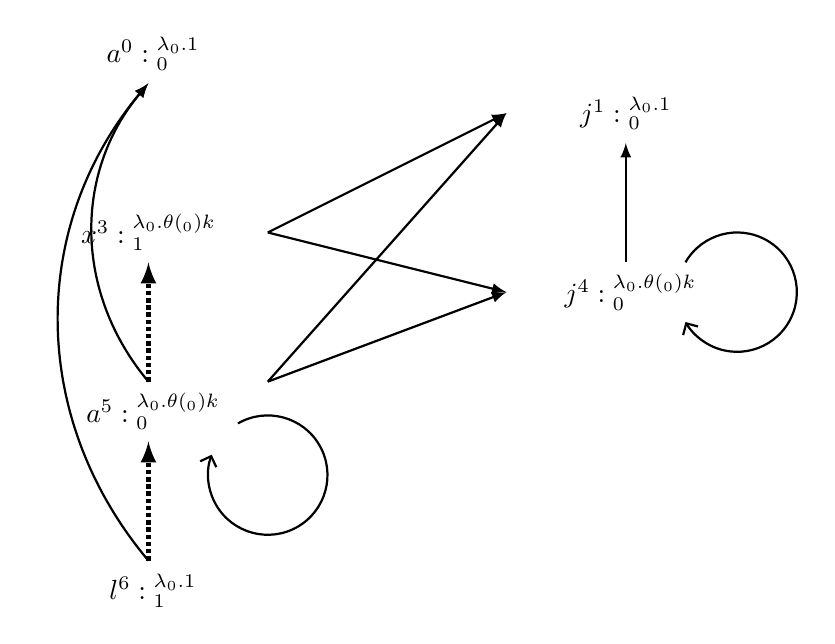
\begin{tikzpicture}[scale=\textwidth/16cm,samples=250]
\draw[] (0, 10) circle (0pt) node
{{ $a^0: {}^{\lambda \trace_0. 1}_{0}$}};
\draw[] (0, 7) circle (0pt) node
{\textbf{$x^3: {}^{\lambda \trace_0. \env(\trace_0) k}_{1}$}};
\draw[] (0, 4) circle (0pt) node {{ $a^5: {}^{\lambda \trace_0. \env(\trace_0) k}_{0}$}};
\draw[] (0, 1) circle (0pt) node
{{ $l^6: {}^{\lambda \trace_0. 1}_{1}$}};
% Counter Variables
\draw[] (8, 9) circle (0pt) node {\textbf{$j^1: {}^{\lambda \trace_0. 1}_{0}$}};
\draw[] (8, 6) circle (0pt) node {{ $j^4: {}^{\lambda \trace_0. \env(\trace_0) k}_{0}$}};
%
% Value Dependency Edges:
\draw[ ultra thick, -latex, densely dotted,] (0, 1.5)  -- (0, 3.5) ;
\draw[ ultra thick, -latex, densely dotted,] (0, 4.5)  -- (0, 6.5) ;
\draw[ thick, -latex] (0, 4.5)  to  [out=-230,in=230]  (0, 9.5) ;
\draw[ thick, -Straight Barb] (1.5, 3.8) arc (120:-200:1);
\draw[ thick, -Straight Barb] (9, 6.5) arc (150:-150:1);
\draw[ thick, -latex] (8, 6.5)  -- (8, 8.5) ;
\draw[ thick, -latex] (0, 1.5)  to  [out=-230,in=230]  (0, 9.5) ;
% Control Dependency
\draw[ thick,-latex] (2, 7)  -- (6, 9) ;
\draw[ thick,-latex] (2, 4.5)  -- (6, 9) ;
\draw[ thick,-latex] (2, 7)  -- (6, 6) ;
\draw[ thick,-latex] (2, 4.5)  -- (6, 6) ;
\end{tikzpicture}
\caption{}
\end{centering}
\end{subfigure}
   \begin{subfigure}{.36\textwidth}
   \begin{centering}
   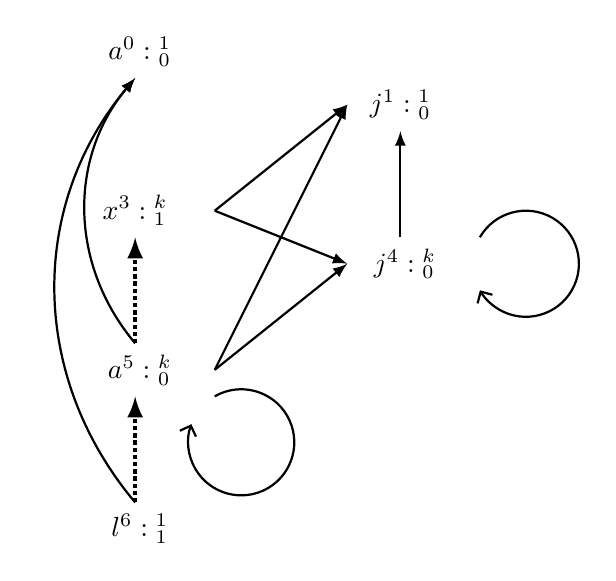
\begin{tikzpicture}[scale=\textwidth/18cm,samples=200]
\draw[] (0, 10) circle (0pt) node
{{ $a^0: {}^1_{0}$}};
\draw[] (0, 7) circle (0pt) node
{\textbf{$x^3: {}^{k}_{1}$}};
\draw[] (0, 4) circle (0pt) node
{{ $a^5: {}^{k}_{0}$}};
\draw[] (0, 1) circle (0pt) node
{{ $l^6: {}^{1}_{1}$}};
% Counter Variables
\draw[] (5, 9) circle (0pt) node {\textbf{$j^1: {}^{1}_{0}$}};
\draw[] (5, 6) circle (0pt) node {{ $j^4: {}^{k}_{0}$}};
%
% Value Dependency Edges:
\draw[ ultra thick, -latex, densely dotted,] (0, 1.5)  -- (0, 3.5) ;
\draw[ ultra thick, -latex, densely dotted,] (0, 4.5)  -- 
% node [left] {\highlight{$\trace_0 \to \env(\trace_0) k $}}
(0, 6.5) ;
\draw[ thick, -latex] (0, 4.5)  to  [out=-230,in=230]  
% node [left] {\highlight{$\trace_0 \to \env(\trace_0) k $}}
(0, 9.5) ;
\draw[ thick, -Straight Barb] (1.5, 3.5) arc (120:-200:1);
\draw[ thick, -Straight Barb] (6.5, 6.5) arc (150:-150:1);
    % The Weight for this edge
    % \draw[](9, 6) node [] {\highlight{$\trace_0 \to \env(\trace_0) k  $}};
\draw[ thick, -latex] (5, 6.5)  -- (5, 8.5) ;
% Control Dependency
\draw[ thick,-latex] (1.5, 7)  -- (4, 9) ;
\draw[ thick,-latex] (1.5, 4)  -- (4, 9) ;
\draw[ thick,-latex] (1.5, 7)  -- (4, 6) ;
\draw[ thick,-latex] (1.5, 4)  -- (4, 6) ;
\draw[ thick, -latex] (0, 1.5)  to  [out=-230,in=230]  (0, 9.5) ;
\end{tikzpicture}
\caption{}
   \end{centering}
   \end{subfigure}
\vspace{-0.4cm}
 \caption{(a) The program $\kw{towRounds(k)}$, an example 
%  of a program 
with two rounds of adaptivity (b) The corresponding execution-based dependency graph (c) The program-based dependency graph from $\THESYSTEM$.
}
\label{fig:overview-example}
% \vspace{-0.8cm}
\end{figure}
}
% \begin{example}[Execution Trace of a Program with While Command].
\\
\[
\ewhile [(x > 0)]{}^0 \edo [x = x - 1]{}^1;
\]
Let $\trace_0 \in \mathcal{T}$ be the initial trace, 
without loss of generalization, let $\env(\trace_0) x = 1$.
\\
By operational semantics rules, we have following evaluation:
  \begin{mathpar}
\inferrule
  {
   \vtrace_0, (x > 0) \barrow \etrue
   \and 
   \event = ((x > 0), 0, 1, \etrue)
  }
  {
  \config{{\ewhile [(x > 0)]{}^0 \edo [x = x - 1]{}^1;, \vtrace_0}}
  \\
  \xrightarrow{} 
  \config{{[x = x - 1]{}^1; \ewhile [(x > 0)]{}^0 \edo [x = x - 1]{}^1;, \vtrace_0 \cdot ((x > 0), 0, 1, \etrue)}}
  }
  ~\textbf{while-t}
\and
\inferrule
  {
  \inferrule
  {
	\config{x - 1, \vtrace_0 \cdot ((x > 0), 0, 1, \etrue)} \aarrow 0
  }
   {
   \config{{[x = x - 1]{}^1;, \vtrace_0 \cdot ((x > 0), 0, 1, \etrue)}}
  \xrightarrow{} 
  \config{{\eskip;, \vtrace_0 \cdot ((x > 0), 0, 1, \etrue) \cdot (x, 1, 1, 0)}}
   }~\textbf{asn}
  }
  {
  \config{{[x = x - 1]{}^1; \ewhile [(x > 0)]{}^0 \edo [x = x - 1]{}^1;, \vtrace_0 \cdot \event}}
  \\
  \xrightarrow{} 
  \config{{\eskip; \ewhile [(x > 0)]{}^0 \edo [x = x - 1]{}^1;, \vtrace_0 \cdot ((x > 0), 0, 1, \etrue) \cdot (x, 1, 1, 0)}}
  }
  ~\textbf{seq1}
\and
\inferrule
  {
  \inferrule
  {
   \vtrace_0, (x > 0) \barrow \efalse
   \and 
   \event = ((x > 0), 0, 2, \efalse)
  }
   {
   \config{{\ewhile [(x > 0)]{}^0 \edo [x = x - 1]{}^1;, \vtrace_0 \cdot ((x > 0), 0, 1, \etrue)}}
  \\
  \xrightarrow{} 
  \config{{\eskip;, \vtrace_0 \cdot ((x > 0), 0, 1, \etrue) \cdot (x, 1, 1, 0)\cdot ((x > 0), 0, 2, \efalse)}}
   }~\textbf{while-f}
  }
  {
  \config{{\eskip; \ewhile [(x > 0)]{}^0 \edo [x = x - 1]{}^1;, \vtrace_0 \cdot ((x > 0), 0, 1, \etrue) \cdot (x, 1, 1, 0)}}
  \\
  \xrightarrow{} 
  \config{{\eskip;, 
  \vtrace_0 \cdot ((x > 0), 0, 1, \etrue) \cdot (x, 1, 1, 0) \cdot ((x > 0), 0, 2, \efalse)}}
  }
  ~\textbf{seq2}
\end{mathpar}
%
Then we have following execution, where $\trace_0 \in \mathcal{T}$ and $\env(\trace_0) x = 1$.:
\[
\config{\ewhile [(x > 0)]{}^0 \edo [x = x - 1]{}^1;, \trace_0}
	\rightarrow^{*}
\config{{\eskip;, 
  \vtrace_0 \cdot ((x > 0), 0, 1, \etrue) \cdot (x, 1, 1, 0) \cdot ((x > 0), 0, 2, \efalse)}}
\]
\end{example}
%
%
\clearpage
\begin{example}[Example of Timing Channel under Trace Semantics].
\label{ex:timingdep}
\\
Using the same example from Example.~\ref{ex:excltiming}
\[
	\ewhile  [(x > 0)]{}^1 \edo [x = x - 1;]{}^2  [y = 1;]{}^3
\]
In this example, $y$'s execution times relies on value of $x$. Under the adaptivity scenario, $y$ depends on $x$ (control dependency).
%
This example shows we can derive by Definition.~\ref{def:var_dep}:
\[
	\vardep(x^2, y^3, {\ewhile  [(x > 0)]{}^1 \edo [x = x - 1;]{}^2  [y = 1;]{}^3})
\]
%
\begin{proof}
Let $\trace_0 = \cdot (x, 0, 1, 2) \in \mathcal{T}$, by semantics definition, we have:
%
\begin{equation}
\label{eq:os_timingdep}
\begin{array}{ll}
& \config{\ewhile [(x > 0)]{}^1 \edo [x = x - 1;]{}^2  [y = 1;]{}^3 , \trace_0} \\
& \rightarrow^\rname{while-t}
\config{[x = x - 1;]{}^2  [y = 1;]{}^3; \ewhile  [(x > 0)]{}^1 \edo [x = x - 1;]{}^2  [y = 1;]{}^3, \trace_0 \cdot ((x > 0), 1, 1, \etrue)} \\
& \rightarrow^\rname{seq1}
\config{[\eskip]{}^2  [y = 1;]{}^3; \ewhile  [(x > 0)]{}^1 \edo [x = x - 1;]{}^2  [y = 1;]{}^3, \trace_0 \cdot ((x > 0), 1, 1, \etrue) \cdot(x, 2, 1, 1)} \\
& \rightarrow^\rname{seq2}
\config{[\eskip]{}^3; \ewhile  [(x > 0)]{}^1 \edo [x = x - 1;]{}^2  [y = 1;]{}^3, \trace_0 \cdot ((x > 0), 1, 1, \etrue) \cdot(x, 2, 1, 1) \cdot(y, 3, 1, 1)} \\
&\rightarrow^\rname{seq2}
\config{[x = x - 1;]{}^2  [y = 1;]{}^3; \ewhile  [(x > 0)]{}^1 \edo [x = x - 1;]{}^2  [y = 1;]{}^3, \trace_0 \cdot ((x > 0), 1, 1, \etrue) \cdot (x, 2, 1, 1) \\
& \quad \cdot(y, 3, 1, 1) \cdot ((x > 0), 1, 2, \etrue)} \\
& \rightarrow^\rname{seq1}
\config{[\eskip]{}^2  [y = 1;]{}^3; \ewhile  [(x > 0)]{}^1 \edo [x = x - 1;]{}^2  [y = 1;]{}^3, \trace_0 \cdot ((x > 0), 1, 1, \etrue) \cdot(x, 2, 1, 1) \\
& \quad \cdot(y, 3, 1, 1) \cdot ((x > 0), 1, 2, \etrue) \cdot(x, 2, 2, 0)} \\
& \rightarrow^\rname{seq2}
\config{[\eskip]{}^3; \ewhile  [(x > 0)]{}^1 \edo [x = x - 1;]{}^2  [y = 1;]{}^3, \trace_0 \cdot ((x > 0), 1, 1, \etrue) \cdot (x, 2, 1, 1) \\
& \quad \cdot(y, 3, 1, 1) \cdot ((x > 0), 1, 2, \etrue) \cdot(x, 2, 2, 0) \cdot(y, 3, 2, 1)} \\
& \rightarrow^\rname{seq2}
\config{[\eskip]{}^1;, \trace_0 \cdot ((x > 0), 1, 1, \etrue) \cdot(x, 2, 1, 1) \\
& \quad \cdot(y, 3, 1, 1) \cdot ((x > 0), 1, 2, \etrue) \cdot(x, 2, 2, 0) \cdot(y, 3, 2, 1) \cdot ((x > 0), 1, 3, \efalse)} \\
\end{array}
\end{equation}
%
Let $\event_1 = (x, 2, 1, 1)$,  $\event_1' = (x, 2, 1, 0)$ and $\event_2 = ((y, 3, 2, 1))$, then we have another execution as follows:
\[
\begin{array}{ll}
& \config{[\eskip]{}^2  [y = 1;]{}^3; \ewhile  [(x > 0)]{}^1 \edo [x = x - 1;]{}^2  [y = 1;]{}^3, \trace_0 \cdot ((x > 0), 1, 1, \etrue) \cdot \event_1'} \\
& \rightarrow^\rname{seq2}
\config{[\eskip]{}^3; \ewhile  [(x > 0)]{}^1 \edo [x = x - 1;]{}^2  [y = 1;]{}^3, \trace_0 \cdot ((x > 0), 1, 1, \etrue) \cdot \event_1' \cdot(y, 3, 1, 1)} \\
&\rightarrow^\rname{seq2}
\config{[\eskip;]{}^1, \trace_0 \cdot ((x > 0), 1, 1, \etrue) \cdot \event_1' \cdot(y, 3, 1, 1) \cdot ((x > 0), 1, 2, \efalse)} \\
\end{array}
\]
%
Then, we have:
\[
\begin{array}{l}
\event_2 \ismin \trace_0 \cdot ((x > 0), 1, 1, \etrue) \cdot \event_1' \cdot(y, 3, 1, 1) \cdot ((x > 0), 1, 2, \etrue) \cdot(x, 2, 2, 0) \cdot(y, 3, 2, 1) \cdot ((x > 0), 1, 3, \efalse)\\
\land
\event_2 \notismin \trace_0 \cdot ((x > 0), 1, 1, \etrue) \cdot \event_1' \cdot(y, 3, 1, 1) \cdot ((x > 0), 1, 2, \efalse)
\end{array}
\]
%
By Definition~\ref{def:event_ctldep}, we have:
%
\[
	\eventdep^{\ctl}(\event_1, \event_2, \ewhile  [(x > 0)]{}^1 \edo [x = x - 1;]{}^2  [y = 1;]{}^3, D)
\]
%
By Definition~\ref{def:event_dep}, we have: 
\[
	\eventdep(\event_1, \event_2, \ewhile  [(x > 0)]{}^1 \edo [x = x - 1;]{}^2  [y = 1;]{}^3, D)
\]
%
By Definition~\ref{def:event_dep}, we have:
\[
	\vardep(x^2, y^3, {\ewhile  [(x > 0)]{}^1 \edo [x = x - 1;]{}^2  [y = 1;]{}^3})
\]
%
\end{proof}
\end{example}
%
\clearpage
\begin{example}[Excluding the Over approximation in Example.~\ref{eq:sem_timingoverapp}].
\\
Consider the same example in Example.~\ref{eq:sem_timingoverapp}, where the dependency is over approximated by Definition~2 (in \cite{cousot2019abstract}):
\[
	\ewhile [(x > 0)] {}^2 [ y = 1;]{}^3 
\]
Let $z^i \in \lvar_{C} \setminus \{x^1\}$ be arbitrary variable different from $x$,
in this example, $y$ doesn't rely on $z$. 
This example shows by the modified data dependency in Definition~\ref{def:var_dep}, the dependency between $z^i$ and $y^3$ cannot be derived.
%
\begin{proof}
%
Without loss of generalization, 
let $\trace_0 \in \mathcal{T}$ be arbitrary initial trace where $\env(\trace_0) x = v$ and $v > 0$.
\\
By operational semantics, let $\trace_j = \cdot ((x > 0), 2, j, \etrue) \cdot(y, 3, j, 1)$ we have:
\[
\label{eq:os_timingdep}
\config{\ewhile  [(x > 0)]{}^2 \edo [y = 1;]{}^3 , \trace_0} \rightarrow^*
\config{[\eskip]{}^1;, \trace_0 \cdot \trace_1 \cdot \trace_2 \cdots}
\]
%
For arbitrary initial trace $\trace_0 \in \mathcal{T}$, there doesn't exist an event $\event$ s.t. 
$(\pi_1(\event), \pi_2(\event)) = (z, i)$ in $\cdot \trace_1 \cdot \trace_2 \cdots$, i.e.,
\[
  \not\exists \event \st (\pi_1(\event), \pi_2(\event)) = (z, i) \land
 \event \ismin \cdot \trace_1 \cdot \trace_2 \cdots
\]
%
Let $\event_y = (y, 3, j, 1)$ for arbitrary $j$, then, by definition of variable dependency, we know:
\[ 
\forall  \event_2 \st (\pi_1(\event_2), \pi_2(\event_2)) = (y, 3) 
\st \not\exists \event_1 \st \pi_1(\event_1) = (z, i) \land \eventdep(\event_z, \event_y)
\]
%
i.e., there isn't dependency relations between $z^i$ and $y^3$ by Definition~\ref{def:var_dep}
\[
  \neg \vardep(z^1, y^3, \ewhile  [(x > 0)]{}^2 \edo [y = 1;]{}^3, D)
\]
\end{proof}
\end{example}
%

\clearpage
% % 
\section{\THESYSTEM}
\label{sec:adpfun}
The adaptivity from the static program analysis result is defined firstly. 
Then the algorithms for {\THESYSTEM}.
{\THESYSTEM} consists of three phases: 
\begin{enumerate}
    \item An algorithm to generate a precise data control flow graph
    \item An algorithm to perform a Reachability number analysis to calculate the weight of each node in the graph generated in phase 1.
    \item An algorithm to find the appropriate path in the weighted data control flow graph
\end{enumerate}
%
\subsection{Adaptivity Based on Program Analysis in \THESYSTEM}
%
\subsubsection{$\flowsto$}
Given a program  ${c}$ with its labelled variables $\lvar_c$,
and two variables ${x^i}, y^j  \in \lvar_c $ 
% showing up as $i$-th, $j$-th elements in $\lvar$ 
% (i.e., ${x} = \lvar(i)$ and ${y} = \lvar(j)$),
we say $y^j$ flows to ${x^i}$ in ${c}$ if and only if 
the value of $y^j$ directly or indirectly influence the evaluation of the value of ${x}$ as follows:
%
\begin{itemize}
\item (Explicit Influence) The program ${c}$ contains either 
a command $[\assign{{x}}{\aexpr}]^i$ or $[\assign{{x}}{\query({\qexpr})}]^i$,
such that ${y}$ shows up as a free variable in $\sexpr$ or ${\qexpr}$.
We use $\flowsto({x^i, y^j, c})$ to denote $y^j$ flows to $x^i$ in ${c}$.
%
\item (Implicit Influence) The program ${c}$ contains either a while loop
command
or if condition command, 
such that $x$ shows up in the guard
and $y$ shows up in the left hand of an assignment command, and this assignment command shows up
 in the body associated to that condition command.
\end{itemize}
%
This is formally defined in \ref{def:flowsto}.
We use $FV(\expr)$, $FV(\sbexpr)$ and $FV(\qexpr)$ denote the set of free variables in 
expression $\expr$, boolean expression $\sbexpr$ and query expression $\qexpr$ respectively.
%
\\
$\live^l(c) \subseteq \lvar_c$ 
is a subset of program $c$'s labelled variables.
For every labelled variable $x^l$ in this set, 
the value assigned to that variable
in the assignment command associated to that label is reachable at the entry point of  executing the command of label $l$.
This is formally defined and computed in the first step of the analysis algorithm.
%
\begin{defn}[Data Flows between Assigned Variables ($\flowsto$)].
\label{def:flowsto}
\\
In a program  ${c}$,
an variable ${x^i}  \in \lvar_c $ is in the \emph{flows to} relation with another variable ${y^j} \in \lvar_c$
in ${c}$, denoted as $\flowsto({x^i, y^j, c})$, is defined as follows:
%
\[
\begin{array}{l}
\flowsto({x^i, y^j, c}) \triangleq 
\\
\left( \bigvee
\begin{array}{l}
(\exists \sexpr . ~ [\assign{y}{\sexpr}]^j \in_{c} {c} 
\land {x} \in VAR(\sexpr) \land (x^i \in \live^j(c)))
\\
(\exists {\qexpr}. ~ [\assign{y}{\query({\qexpr})}]^j \in_{c} {c} 
\land x \in VAR({\qexpr}) \land (x^i \in \live^j(c))))
\\
\big(\exists  ~ {c_w}, {(\expr \lor \qexpr)}, \sbexpr, l \in \mathbb{N}. ~
	\ewhile [\sbexpr]^l \edo {c_w} \in_{c} {c}
	\land 
	[{\assign{y}{\expr \lor \query(\qexpr)}}]^{j} \in_{c}  {c_w}
\big) \land {x} \in VAR(\sbexpr) \land (x^i \in \live^l(c)))
\\
\big(
\exists ~ \sbexpr, l \in \mathbb{N}, {c_1}, {c_2}, {\expr}_1, {\expr}_2. ~
	\eif([\sbexpr]^l, {c_1}, {c_2}) \in_{c} {c} \land
	([{\assign{y}{\expr_1}}]^j \in_{c} {c_1} \lor 
	[{\assign{y}{\expr_2}}]^j \in_{c} {c_2})
\land {x} \in VAR(\sbexpr) \land (x^i \in \live^l(c)))
\big)
% \\
% (\exists z^r \in \lvar_c \st \flowsto(x^i, z^r, c) \land \flowsto(z^r, y^j, c))
\end{array}
\right).
\end{array}
\]
%
\end{defn}
%
Program Entry Point: $\entry_c : \mbox{Command} \to \mathbb{N}$ 
\[
  \entry_c \triangleq 
\left\{
  \begin{array}{ll} 
     l       
    & c = [\eskip]{}^l
    \\ 
    l    & c = [\assign{x}{\expr_1}]{}^l
    \\ 
    l      
    & c = [\assign{x}{\query(\qexpr_1)}]{}^l
    \\
   l
    & c_1 = \eif([b]{}^l, c_t, c_f)
    \\ 
    l         
    & c = \ewhile [b]^l \edo c'
    \\ 
    \entry_{c1}
    & c = c1;c2
  \end{array}
  \right.
\]
%
\begin{defn}[Equivalence of Program]
%
\label{def:aq_prog}
Given 2 programs $c_1$ and $c_2$:
\[
c_1 =_{c} c_2
\triangleq 
\left\{
  \begin{array}{ll} 
    \etrue        
    & c_1 = \eskip \land c_2 = \eskip
    \\ 
    \forall \trace \in \mathcal{T} \st \exists v \in \mathcal{VAL}
    \st \config{ \trace, \expr_1} \aarrow v \land \config{ \trace, \expr_1} \aarrow v     
    & c_1 = \assign{x}{\expr_1} \land c_2 = \assign{x}{\expr_2} 
    \\ 
    \qexpr_1 =_{q} \qexpr_2       
    & c_1 = \assign{x}{\query(\qexpr_1)} \land c_1 = \assign{x}{\query(\qexpr_2)} 
    \\
    c_1^f =_{c} c_2^f \land c_1^t =_{c} c_2^t
    & c_1 = \eif(b, c_1^t, c_1^f) \land c_2 = \eif(b, c_2^t, c_2^f)
    \\ 
    c_1' =_{c} c_2'         
    & c_1 = \ewhile b \edo c_1' \land c_2 = \ewhile b \edo c_2'
    \\ 
    c_1^h =_{c} c_2^h \land c_1^t =_{c} c_2^t
    & c_1 = c_1^h;c_1^t \land c_2 = c_2^h;c_2^t 
  \end{array}
  \right.
\]
%
$c_1 \neq_{c} c_2$  is defined vice versa.
%
\end{defn}
%
Given 2 programs $c$ and $c'$, $c'$ is a sub-program of$c$, i.e., $c' \in_{c} c$ is defined as:
\begin{equation}
c' \in_{c} c \triangleq \exists c_1, c_2, c''. ~ s.t.,~
c =_{c} c_1; c''; c_2 \land c' =_{c} c''
\end{equation} 
%

\subsubsection{Program Analysis Based Dependency Graph}
\begin{defn}
    [Program-Based Dependency Graph].
    \label{def:prog_graph}
    \\
Given a program ${c}$
its program-based graph 
$\progG({c}) = (\vertxs, \edges, \weights, \flag)$ is. defined as:
\\
\[
\begin{array}{rlcl}
\text{Vertices} &
\vertxs & := & \left\{ 
x^l \in \mathcal{VAR} \times \mathbb{N}
~ \middle\vert ~
x^l \in \lvar({{c}})
\right\}
\\
\text{Directed Edges} &
\edges & := & 
\left\{ 
  ({x}_1^{i}, {x}_2^{j}) \in \mathcal{VAR} \times \mathbb{N} \times (\mathcal{VAR} \times \mathbb{N})
  ~ \middle\vert ~
  \begin{array}{l}
    {x}_1^{i}, {x}_2^{j} \in \vertxs
	\land
    \\
    \exists n \in \mathbb{N}, z_1^{r_1}, \cdots, z_n^{r_n} \in \lvar_{{c}} \st 
    n \geq 0 \land
    \\
    \flowsto(x^i,  z_1^{r_1}, c) 
    \land \cdots \land \flowsto(z_n^{r_n}, y^j, c) 
  \end{array}
\right\}
\\
\text{Weights} &
\weights & := &
% \bigcup
% \begin{array}{l}
	\big\{ (x^l, w) \in \mathcal{VAR} \times \mathbb{N} \times (\mathbb{N} \cup \aexpr)
	\mid
	x^l \in \lvar_{{c}} \land w = \rb(x^l, c)
	\big\} 
	% \\
	% \big\{(x^l, 1)  \in \mathcal{VAR} \times \mathbb{N} \times \{1\} 
	% \mid
	% x^l \in \lvar_{{c}} \land \flag(x^l) = 0
	\big\}
% \end{array} 
\\
\text{Query Flags} &
\qflag & := & 
\left\{(x^l, n)  \in \mathcal{VAR} \times \mathbb{N}  \times \{0, 1\} 
~ \middle\vert ~
 x^l \in \lvar_{c},
 \left\{
\begin{array}{ll}
n = 1 & x^l \in \qvar_{c} \\ 
n = 0 & o.w.
\end{array}
\right\}
\right\}
\end{array}
\]
%
\[
\begin{array}{rlcl}
\text{Vertices} &
\vertxs & := & \left\{ 
x^l 
~ \middle\vert ~
x^l \in \lvar_{{c}}
\right\}
\\
\text{Directed Edges} &
\edges & := & 
\left\{ 
  ({x}_1^{i}, {x}_2^{j}) 
  ~ \middle\vert ~
  \begin{array}{l}
    {x}_1^{i}, {x}_2^{j} \in \lvar_{{c}},
    \\
    \exists n \in \mathbb{N}, z_1^{r_1}, \cdots, z_n^{r_n} \in \lvar_{{c}} \st 
    n \geq 0 \land
    \\
    \flowsto(x^i,  z_1^{r_1}, c) 
    \land \cdots \land \flowsto(z_n^{r_n}, y^j, c) 
  \end{array}
\right\}
\\
\text{Weights} &
\weights & := &
% \bigcup
% \begin{array}{l}
	\big\{ (x^l, w)
	\mid
	x^l \in \lvar_{{c}}, w = \rb(x^l, c)
	\big\} 
	% \\
	% \big\{(x^l, 1)  \in \mathcal{VAR} \times \mathbb{N} \times \{1\} 
	% \mid
	% x^l \in \lvar_{{c}} \land \flag(x^l) = 0
	\big\}
% \end{array} 
\\
\text{Query Flags} &
\qflag & := & 
\left\{(x^l, n)   
~ \middle\vert ~
 x^l \in \lvar_{c},
 x^l \in \qvar_{c} \implies n = 1,
 x^l \notin \qvar_{c} \implies n = 0
%  \left\{
% \begin{array}{ll}
% n = 1 & x^l \in \qvar_{c} \\ 
% n = 0 & o.w.
% \end{array}
% \right\}
\right\}
\end{array}
\]
\end{defn} 
%
Given a program ${c}$, we generate its program-based graph 
$\progG({c}) = (\vertxs, \edges, \weights, \qflag)$.
%
Then the adaptivity bound based on program analysis for ${c}$ is the number of query vertices on a finite walk in $\progG({c})$. This finite walk satisfies:
\begin{itemize}
\item the number of query vertices on this walk is maximum
\item the visiting times of each vertex $v$ on this walk is bound by its reachability bound $\weights(v)$.
\end{itemize}
It is formally defined in \ref{def:prog_adapt}.
%
%
\begin{defn}
[{Program-Based Adaptivity}].
\label{def:prog_adapt}
\\
{
Given a program ${c}$ and its program-based graph 
$\progG({c}) = (\vertxs, \edges, \weights, \qflag)$,
%
the program-based adaptivity for $c$ is defined as%
\[
\progA({c}) 
:= \max
\left\{ \qlen(k)\ \mid \  k\in \walks(\progG({c}))\right \}.
\]
}
\end{defn}  
%
%
% {
% \begin{defn}[Variable Flags ($\flag$)].
% \\
% Given a program  ${c}$ with its labelled variables $\lvar$, the $\flag$ is a vector of the same length as $\lvar$, s.t. for each variable ${x}$ showing up as the $i$-th element in $\lvar$ (i.e., ${x} = \lvar(i)$), 
% $\flag(i) \in \{0, 1, 2\}$ is defined as follows:
% %
% %
% \[
% \flag(i) := 
% \left\{
% \begin{array}{ll}
% 2 & 
% {x^l} \in \lvar_{c} \land 
% (\exists {\qexpr}. ~ s.t., ~
% [\assign{{x}}{\query({\qexpr})}]^l \in_{c} {c})
% \\
% 1 &  
% \begin{array}{l}
% {x^l} \in \lvar_{c} \bigwedge \\
% \left(
% \begin{array}{l}
% \big(\exists  ~ {c'}, {\expr}, \sbexpr, l, l'. ~
% 	\ewhile [\sbexpr]^l \edo {c'} \in_{c} {c}
% 	\land 
% 	[{\assign{x}{\expr}}]^{l'} \in_{c}  {c'}
% \big) \bigvee
% \\
% \big(\exists ~ \sbexpr, l, l_1, l_2, {c_1}, {c_2}, {\expr}_1, {\expr}_2. ~
% 	\eif([\sbexpr]^l, {c_1}, {c_2}) \in_{c} {c} \land
% 	([{\assign{x}{\expr_1}}]^{l1} \in_{c} {c_1} \lor 
% 	[{\assign{x}{\expr_2}}]^{l2} \in_{c} {c_2})
% \big)
% \end{array}
% \right)
% \end{array}
% \\
% 0 & \text{o.w.}
% \end{array}
% \right\}. 
% \] 
% %
% \end{defn}
%
% Operations on $\flag$ are defined as follows:
% \begin{equation}
% \begin{array}{llll}
% {\flag_1 \uplus \flag_2}(i) & := &
% \left\{
% \begin{array}{ll}
% k & k = \max{\big\{\flag_1(i), \flag_2(i)\big\}} 
% \land |\flag_1| = |\flag_2|\\
% 0 & o.w.
% \end{array}\right.
% & i = 1, \cdots, |\flag_1|  
% \\
% {\flag \uplus n}(i) & := & 
% \max\big\{ \flag(i), n \big\} 
% & i = 1, \ldots, |\flag|    
% \\
% \left[ n \right]^k (i) & := &  n
% & i = 1, \ldots, k ~ \land ~ |\left[ n \right]^k| = k
% \end{array}
% \end{equation}
%
%
%
% \begin{defn}[Data Flow Matrix ($\Mtrix$)]
% The data flow matrix $\Mtrix$ of a program $c$ is a matrix of size $|\lvar_c| \times |\lvar_c|$ 
% s.t.,
% %
% \[
% \Mtrix(i, j) \triangleq
% \left\{
% \begin{array}{ll}
% 1	&	\flowsto({x^i, y^j, c}) \\
% 0	& o.w.
% \end{array}
% \right., {x^i}, y^j  \in \lvar_c.
% \]
% %
% \end{defn}
% %
% Operations on the data flow matrices are defined as follows:
% %
% \begin{equation}
% \Mtrix_1 ; \Mtrix_2 
% := \Mtrix_2 \cdot \Mtrix_1 + \Mtrix_1 + \Mtrix_2
% \end{equation}
% %
% Consider the same program $c$ as above, its data flow matrix $\Mtrix$ and $\flag$ for the program $c$ is as follows:
% $$
% {c} = 
% \begin{array}{l}
% \left[{\assign {x_1} {\query(0)}}	\right]^1;
% \\
% \left[{\assign {x_2} {x_1 + 1}}		\right]^2;
% \\
% \left[{\assign {x_3} {x_2 + 2}}		\right]^3
% \end{array}
% ~~~~~~~~~~~~
% \Mtrix
% =  \left[ 
% \begin{matrix}
% 0 & 0 & 0 \\
% 1 & 0 & 0 \\
% 1 & 1 & 0 \\
% \end{matrix} \right] ~ , 
% \flag = \left [ \begin{matrix}
% 1 \\
% 0 \\
% 0 \\
% \end{matrix} \right ]
% $$
% %
% % There are two special matrices used for generating the data flow matrix $\Mtrix$ in the analysis algorithm. They are the left matrix $\lMtrix_i$ and right matrix $\mathsf{R_{(e, i)}}$.

% % Given a program  ${c}$ with its labelled variables $\lvar$ of length $N$,
% % the left matrix $\lMtrix_i$ generates a matrix of $1$ column, $N$ rows, 
% % where the $i$-th row is $1$ and all the other rows are $0$.
% % %
% % \begin{defn}[Left Matrix ($\lMtrix_i$)].
% % \\
% % Given a program  ${c}$ with its labelled variables $\lvar$ of size $N$, 
% % the left matrix $\lMtrix_i$ is defined as follows:
% % \[
% % \lMtrix_i(j) : = 
% % \left
% % \{
% % \begin{array}{ll}
% % 1 & j = i \\
% % 0 & o.w.
% % \end{array}
% % \right.,
% % j = 1, \ldots, N.
% % \]
% % \end{defn}
% % %
% % Given a program  ${c}$ with its labelled variables $\lvar$ of length $N$,
% % the right matrix $\rMtrix_{\expr, i}$ generates a matrix of one row and $N$ columns, 
% % where the locations of free variables in $\expr$ is marked as $1$. 
% % %
% % %
% % \begin{defn}[Right Matrix ($\rMtrix_{\expr}$)].
% % \\
% % Given a program  ${c}$ with its labelled variables $\lvar$ of length $N$, 
% % the right matrix $\rMtrix_{\expr}$ is defined as follows:
% % \[
% % \rMtrix_{\expr}(j) : = 
% % \left\{
% % \begin{array}{ll}
% % 1 & {x} \in FV(\expr) 
% % \\
% % 0 & o.w.
% % \end{array}
% % \right.,
% % {x} = \lvar(j) ~ , ~ j = 1, \ldots, N.
% % \]
% % %
% % %
% % \end{defn}
% % %
% % Using the same example program ${c}$ as above with labelled variables $\lvar = [ {x_1 , x_2 , x_3} ] $,
% % the left and right matrices w.r.t. its $2$-nd command 
% % $\left[{\assign {x_2} {x_1 + 1}}\right]^2$  are as follows:
% % \[
% % \lMtrix_1 = \left[ \begin{matrix}
% % 0   \\
% % 1 	 \\
% % 0   \\
% % \end{matrix}   \right ] 
% % ~~~~~~~~~~~~~~
% % \rMtrix_{{x}_1 + 1}
% % = \left[ \begin{matrix} 
% % 1 & 0 & 0 \\
% % \end{matrix}  \right]
% % \]
% %
% %
% %
\subsection{ $\THESYSTEM$ Analysis Algorithm}
\wq{To do: Add $\THESYSTEM$, a data flow analysis algorithm to scan the program and give a graph.}
{\THESYSTEM} consists of three phases: 
\begin{enumerate}
    \item An algorithm to generate a precise data control flow graph
    \item An algorithm to perform a Reachability number analysis to calculate the weight of each node in the graph generated in phase 1.
    \item An algorithm to find the appropriate path in the weighted data control flow graph
\end{enumerate}

To be precise, we show the details. 
\subsubsection{Phase 1, precise data control flow graph}
There are 3 steps to generate the graph in this phase.
\begin{enumerate}
\item Generation of control flow graph
    \item Reaching definition analysis
   \item  data-control flow analysis
\end{enumerate}

\paragraph{Generate CFG}
 Define $\mathsf{init}$: Command -> label, which returns the initial label of the statement. 
 \[
 \begin{array}{ll}
    init([x := e]^{l})  & = l  \\
     init([x := q(e)]^{l})  & = l \\
     init([skip]^{l})  & = l \\
     init([if [b]^l then C_1 else C_2]^{l})  & = l \\
     init([while [b]^l do C]^{l})  & = l \\
     init(C_1 ; C_2)  & = init(C_1) \\
 \end{array}
 \]
  Define $\mathsf{final}$: Command -> Powerset(label), which returns the final labels of the statement. 
 \[
 \begin{array}{ll}
    final([x := e]^{l})  & = \{l\}  \\
     final([x := q(e)]^{l})  & = \{l\}  \\
     final([skip]^{l})  & = \{l\} \\
     final([if [b]^l then C_1 else C_2]^{l})  & = final(C_1) \cup final(C_2) \\
     final([while [b]^l do C]^{l})  & = \{l\} \footnote{while terminates after b evaluates to false} \\
     final(C_1 ; C_2)  & =  final(C_2) \\
 \end{array}
 \]
 Define block B to be either the command of the form of assignment, skip, or test of the form of $[b]^{l}$.\\
 Define $\mathsf{blocks}$ : command -> Powerset(Block)
 \[
 \begin{array}{ll}
    blocks([x := e]^{l})  & = \{[x := e]^{l}\}  \\
     block([x := q(e)]^{l})  & = \{[x := q(e)]^{l}\}  \\
     blocks([skip]^{l})  & = \{[skip]^{l}\} \\
     blocks([if [b]^l then C_1 else C_2]^{l})  & = {[b]^{l}} \cup blocks(C_1) \cup blocks(C_2) \\
     blocks([while [b]^l do C]^{l})  & = \{[b]^{l}\} \cup blocks(C) \\
     blocks(C_1 ; C_2)  & = blocks(C_1) \cup  blocks(C_2) \\
 \end{array}
 \]
 Define $\mathsf{labels}$ to get the labels of blocks.
 \[
   labels(C) = \{l | [B]^{l} \in blocks(C) \}
 \]  

The control flow graph is generated by edges between labels. Define $\mathsf{flow}$: command -> P (label $\times$ label ).

\[
 \begin{array}{ll}
    flow([x := e]^{l})  & = \emptyset  \\
     flow([x := q(e)]^{l})  & = \emptyset  \\
     flow([skip]^{l})  & = \emptyset \\
     flow([if [b]^l then C_1 else C_2)  & =  flow(C_1) \cup flow(C_2)\cup \{(l, init(C_1)) , (l, init(C_2)) \} \\
     flow([while [b]^l do C)  & =  flow(C) \cup \{(l, init(C)) \} \cup \{(l', l)| l' \in final(C) \} \\
     flow(C_1 ; C_2)  & = flow(C_1) \cup  flow(C_2) \cup \{ (l,init(C_2)) | l \in final(C_1) \} \\
 \end{array}
 \]
 
 \paragraph{Reaching definition analysis}
 Set $?$ to be undefined, $label^{?}$ is label $\cup \{?\}$.\\
 Define $\mathsf{kill}$: blocks -> Powerset(Var $\times$ $label^l$, which produces the set of labelled variables of assignment destroyed by the block.\\
 Define $\mathsf{gen}$: blocks->Powerset(Var $\times$ $label^l$, which generates the set of labelled variables generated by the block.\\
 Define $defs(x)(C)$: Var -> Set of labels, gives all the labels where assigns value to variable x in the target program C.
  \[
 \begin{array}{ll}
    kill([x := e]^{l})  & = \{ (x, ?) \} \cup \{ (x, l') | l' \in defs(x) \} \\
     kill([x := q(e)]^{l})  & = \{ (x, ?) \} \cup \{ (x, l') | l' \in defs(x) \}  \\
     kill([skip]^{l})  & = \emptyset \\
     kill([ [b]^l ]^{l})  & =  \emptyset \\
      gen([x := e]^{l})  & = \{ (x, l) \}  \\
     gen([x := q(e)]^{l})  & = \{ (x, l) \}  \\
     gen([skip]^{l})  & = \emptyset \\
     gen([ [b]^l ]^{l})  & =  \emptyset 
 \end{array}
 \]
 Define $in(l)$, $out(l)$: label -> (var $\times$ $label^l$) for the entry point and exit point of the node $l$ in the control flow graph.
 \[
 \begin{array}{lll}
    in(l)  & = \{ (x, ?) | x is assigned in C  \} & l = init(C)\\
    & \cup \{ out(l')|  | (l',l) \in flow(C) \} & ow \\
     out(l)  & =  gen(B^{l}) \cup \{ in(l) \setminus kill(B^l)  \} & B^l \in blocks(C)   
 \end{array}
 \]
 
The Reaching definition is calculated by the Worklist algorithm as below.
\begin{enumerate}
    \item initial in[l]=out[l]=$\emptyset$
    \item initial in[entry label] = $\emptyset$
    \item initialize a work queue, contains all the blocks in C
    \item while |W| != 0 \\
         pop l in W\\
          old = out[l]\\
          in(l) =  out(l') where (l',l) in flow(C)\\
           out(l) = gen($b^l$) $\cup$ (in(l) - kill($b^l$) ) where $b^l$ in block(C)   \\
          if (old != out(l)) W= W $\cup$ \{l'| (l,l') in flow(C)\}\\
          end while
\end{enumerate}

 \paragraph{control-data flow graph}
 We build this graph by using the results of Reaching definition analysis, to be specific, in(l) for every label. 
 
 Define dcgd: Command -> Labelled VAR $\times$ 
 Labelled VAR. dcgd is short for data control
 dependency graph. $RD_{in}$ is the result of reaching definition in last step. 
 
  \[
 \begin{array}{ll}
    dcdg([x := e]^{l})  & = \{ (y^i, x^l) | y \in VAR(e) \land (y,i) \in RD_{in}(l) \}  \\
     dcdg([x := q(e)]^{l})  & = \{ (y^i, x^l) | y \in VAR(e) \land (y,i) \in RD_{in}(l) \}  \\
     dcdg([skip]^{l})  & = \emptyset \\
     dcdg([if [b]^l then C_1 else C_2)  & =  dcdg(C_1) \cup dcdg(C_2)\\ & \cup \{(x^i,y^j) | x \in VAR(b) \land (x,i) \in RD_{in}(l) \land ([y = \_]^j) \in blocks(C_1) \} \\
     &\cup \{(x^i,y^j) | x \in VAR(b) \land (x,i) \in RD_{in}(l) \land ([y = \_]^j) \in blocks(C_2) \} \\
     dcdg([while [b]^l do C)  & =  dcdg(C) \cup \{(x^i,y^j) | x \in VAR(b) \land (x,i) \in RD_{in}(l) \land ([y = \_]^j) \in blocks(C) \} \\
     dcdg(C_1 ; C_2)  & = dcdg(C_1) \cup  dcdg(C_2) \\
 \end{array}
 \]
 
 

\subsubsection{Phase 2, reachability number analysis}

In last phase, we get a dependency graph whose node is computation blocks uniquely decided by its label. In this phase, we want to add more information to every node in the graph, which is the approximated visiting times (how many times this block is exeucted). The algorithm is defined in Algorithm~\ref{alg:add_weights}, with 3 main functions, the PREPROCESSING, $\rb$ and ADDWEIGHT. 
\begin{algorithm}
\caption{
{Add weights to dependency graph (the main algorithm of phase 2)}
\label{alg:add_weights}
}
\begin{algorithmic}[1]
\REQUIRE the program $c$, the dependency graph $G = (\vertxs, \edges, \weights, \qflag)$ from phase 1
\STATE  prel = PREPROCESSING(c) 
\STATE {\bf for} $x^l \in \vertxs$: 
\STATE \qquad {\bf if} $l \in prel$:
\STATE \qquad \qquad $\weights(x^l) = \rb(c, l)$
\STATE \qquad {\bf else}:
\STATE \qquad \qquad $\weights(x^l) = 1$
\RETURN $G$
\end{algorithmic}
\end{algorithm}

\paragraph{Preprocessing} This step is straightforward. Since variable's visiting time outside of any while loop is at most 1, we do not need to analyze the visiting times of every node in the graph from phase 1.
We have a pre-processing algorithm to go through the programs and returns the list of labels associating with a loop and whose visiting times need to be analyzed.

\paragraph{Getting Reachability Bounds}
This is defined in Algorithm~\ref{alg:rb}.
To be precise, we use static analysis method from \cite{Sumit2010rechability}, which is able to "provide the symbolic worst case bound on the number of times a block is reached", let us call it reachability bound analysis. 

This analysis only works to find the symbolic bound of one block (in our graph, it corresponds to one node). This algorithm is summarized as follows.
\begin{enumerate}
    \item Build a transition system which describes the relation between variables in this target block and these variables in the successive visit to this block. There are defined translate functions which translate the statement to transition system and the corresponding operations such as the composition of transition systems, merging two transition systems from two control branches and so on. It is worth to mention that it calculates the transitive closure of the transition system obtained from a loop body, which can be analogy to computing the invariant of a loop.  
    \item Use Ranking function which takes the transition system and outputs the bound
\end{enumerate}

\begin{algorithm}
\caption{
{Reachability Bound Analysis ($\rb$)}
\label{alg:rb}
}
\begin{algorithmic}[1]
\REQUIRE the program $C$, the target while loop with label $l$.
\STATE  T  = GenerateTransitionSystem(C,l) 
\STATE B = 1 + ComputeBound(T)
\RETURN B
\end{algorithmic}
\end{algorithm}

The algorithm $GenerateTransitionSystem(C,l)$ can be described as follows. It uses the control flow graph generated from the program $C$, and splits the node marked by $l$ into two nodes $l_1$ and $l_2$ to generate a new control flow graph from the $l_1$ to $l_2$. It translates the node in the graph into a transition systems by the its translate function and replaces node with transition systems. For loops in the graph, the loop itself is replaced by the transitive closure of the transition systems of its body. Finally, the new generated control flow graph can be transformed to a transition system. The transition system is a disjunction of transitions, and every transition is expressed as a conjuction of formulas over program variables $x,y,z$ in the target block (l) and its successive visits $x',y',z'$ in the same block.
\\
The transition formula for each command are as follows:
\\
\todo{adding the naive transition formula for assignment and if}
\\
\jl{$translate(c)$  is defined as follows:}
\\
$translate(\assign{x}{e}) = \{x := e\} if x \in VAR(b)$
\\
% $translate(\assign{x}{e}) = \{\} if x \notin VAR(b)$
% \\
$translate(\assign{x}{\qexpr}) = \{x \in VAR(b) \implies x := \qexpr\} $
\\
% $translate(\assign{x}{\qexpr}) = \{\} if x \notin VAR(b)$
% \\
$translate(\eif(\bexpr, c_1, c_2)) = \{\bexpr \implies translate(c_1), \neg\bexpr \implies translate(c_2)\}$
\\
$translate(\ewhile(\bexpr, c_w)) = \{ ComputeBound(GenerateTransitionSystem(C,l)) \times translate(c_w) \}$
\\
$translate(c_1;c_2) = translate(c_1) + translate(c_2)$
\\
\todo{adding the compose method for composing 2 transition formulas}
$compose\{x := e_1, \cdots, x := e_2 \} = \{x := e_2\}$
\\
$\{y := e_1, \cdots, x := e_2 \} \land \flowsto(y, x, c) = \{x := [y \to e_1] e_2\}$
\\
\todo{add the $ComputeBound$ function, specifically the ranking function}
\\
The function $computeBound$ takes into a transition system (a disjuction of transitions), and computes the bound. There are ranking functions which take a transition and return the bound, that is used by $computeBound$. There are some heuristics in compute the bound based on the transitions systems, if interested, please look at the paper for more details.

\paragraph{Add Weight} We also need to take care about the situation when a bound can not be predicted by {$\rb$}, we need to use another loose analysis to get a loose bound.



\clearpage
\subsubsection{Phase 3, path finding algorithm in weighted graph (graph in phase 1 with weights predicted in phase 2) }
A combination of DFS and BFS Algorithm:
\begin{algorithm}
    \caption{
    {Longest Adaptivity Search Algorithm ($\pathsearch$)}
    \label{alg:adpt_alg}
    }
    \begin{algorithmic}[1]
    \REQUIRE $G = (\vertxs, \edges, \weights, \qflag)$ \#\{A Symbolic Weighted Directed Graph\}
    % with a start vertex $s$ and destination vertex $t$ .
    \STATE  {\bf {$\kw{\pathsearch(G)}$}:}  
    \STATE {\bf init} 
    % \\
    % current node: $c$, 
    \\
    $q$: empty queue.
    % \\
    % $\kw{visited}$: List of length $|\vertxs|$, initialize with $\efalse$.
    % \\
    % $\kw{SSCvisited}$: List of length $|\vertxs|$, initialize with $\efalse$.
    % \\ 
    % $\kw{adapt_{scc}(SCC_i) = \pathsearch_{scc}(SCC_i)}$.
    \\
    $\kw{adapt}$ : the adaptivity of this graph initialize with $0$.
    \\
    \STATE Find all Strong Connected Components (SCC) in $G$: $\kw{SCC_1}, \cdots, \kw{SCC_n}, 0 \leq n \leq |\vertxs|$, where $\kw{SCC_i} = (\vertxs_i, \edges_i, \weights_i, \qflag_i)$.
    % and assign each vertex $x^i$ with an SCC number $\kw{SCC}(x^i)$
    \STATE {\bf for} every SCC: $\kw{SCC_i}$, compute its Adaptivity $\kw{SCC_i}$:
    \STATE \quad $\kw{adapt_{scc}[SCC_i] = \pathsearch_{scc}(SCC_i)}$;
    \STATE {\bf for} every vertex $\kw{SCC_i}$:
    \STATE \qquad $q.append(\kw{SCC_i})$;
    \STATE \qquad $\kw{adapt_{tmp}} = 0$;
    \STATE \qquad {\bf while} $q$ isn't empty:
    \STATE \qquad \qquad $\kw{SCC}= q.pop()$;  \#\{take the top SCC from head of queue\}
    \STATE \qquad \qquad  $\kw{adapt_{tmp}}_0= \kw{adapt_{tmp}}$; \#\{record the adaptivity of last level\}
    \STATE \qquad \qquad  $\kw{SCC_{max}}$;  \#\{record the SCC with longest walk in this level\}
    % initialize cycle-adapt = 0.
    \STATE \qquad \qquad {\bf for} all children SCC of $\kw{SCC}$: $\kw{SCC'}$:
    % \STATE \qquad \qquad   cycle-adapt$ = \max($cycle-adapt, $\kw{dfs_{refine}(G, v, v)})$;
    % \STATE \qquad \qquad \qquad \#\{compute the adaptivity of vertex $v$  on $\kw{SCC}(v)$, and update r[v] with the SCC-adapt\}
    % \STATE \qquad \qquad \qquad $ r[v] = r[s] + \kw{dfs_{refine}(G, v, visited)})$; 
    \STATE \qquad \qquad \qquad {\bf if} $(\kw{adapt_{tmp}} < \kw{adapt_{tmp}}_0 + \kw{adapt_{scc}(SCC')})$:
    \STATE \qquad \qquad \qquad \qquad $\kw{adapt_{tmp}} = \kw{adapt_{tmp}}_0 + \kw{adapt_{scc}[SCC']}$; 
    \STATE \qquad \qquad \qquad \qquad $\kw{SCC_{max} = SCC'} $; \#\{update the SCC with longest walk in this level\} 
    % \STATE \qquad   $r[c] = r[c] + $cycle-adapt;
    % \STATE \qquad for all unvisited vertex $v$ having directed edge from c and $! \kw{cycle}(c)$:
    % \STATE \qquad \qquad $r[v] = r[c] + \flag(v)$; 
    % \STATE \qquad \qquad \qquad  \#\{mark all the nodes with the same $\kw{SCC}$ number as visited\} 
    % \STATE \qquad \qquad \qquad  \#\{append the unvisited vertex to the rear of the queue\}
    % \STATE \qquad \qquad \qquad  \#\{mark all the nodes with the same $\kw{SCC}$ number as visited\} 
    % \STATE \qquad \qquad for $v \in V$,   $\kw{visited}[s] = 1$;
    \STATE \qquad \qquad \qquad $q.append(\kw{SCC_{max}})$;
    \STATE \qquad $\kw{adapt} = \max(\kw{adapt}, \kw{adapt_{tmp}})$;    
    \RETURN $\kw{adapt}$.
    \end{algorithmic}
    \end{algorithm}
    %
    %
    % \begin{algorithm}
    % \caption{
    % {Longest Adaptivity Search Algorithm ($\pathsearch$)}
    % \label{alg:adpt_alg}
    % }
    % \begin{algorithmic}
    % \REQUIRE Weighted Directed Graph $G = (\vertxs, \edges, \weights, \flag)$ with a start vertex $s$ and destination vertex $t$ .
    % \STATE  {\bf {bfs $(G)$}:}  
    % \STATE {\bf init} 
    % \\
    % current node: $c$, 
    % \\
    % queue: $q$ : List, add into $a$ an arbitrary v from $\vertxs$. 
    % \\
    % visited: List of length $|\vertxs|$, initialize with $\efalse$.
    % \\
    % results: $r$ : List of length $|\vertxs|$, initialize with -1.
    % \\
    % curr$\kw{flowcapacity}$: INT, initialize MAXINT.
    % \\
    % querynum: INT, initialize 0. \#\{To count the query numbers when we are walking inside a cycle\}
    % \\
    % \STATE \qquad {\bf while} $q$ isn't empty:
    % \STATE \qquad \qquad take the vertex from head $c= q.pop()$
    % \STATE \qquad \qquad mark $c$ as visited, visited $[c] = 1$.
    % \STATE \qquad \qquad {\bf if} $\kw{cycle}(c)$  \#\{we are inside a cycle\}
    % \STATE \qquad \qquad \qquad curr$\kw{flowcapacity}$ = min($\weights$(c), curr$\kw{flowcapacity}$).
    % \STATE \qquad \qquad \qquad querynum += $\flag(c)$.
    % \STATE \qquad \qquad  \qquad for all unvisited vertex $v$ having directed edge from c:
    % \STATE \qquad \qquad \qquad \qquad r[v] = r[c]; q.add(v)
    % \STATE \qquad \qquad \qquad  {\bf if}  $v$ is visited, then the circle finished
    % \STATE \qquad \qquad \qquad \qquad update the result $r[v] =  \max(r[v], r[c] + $curr$\kw{flowcapacity}$*querynum)
    % \STATE \qquad \qquad \qquad \qquad curr$\kw{flowcapacity}$ = MAXINT
    % \STATE \qquad \qquad \qquad \qquad querynum = 0.  
    % \STATE \qquad \qquad {\bf else} 
    % \STATE \qquad \qquad \qquad for all unvisited vertex $v$ having directed edge from c:
    % \STATE \qquad \qquad \qquad  \qquad $r[v] = \max(r[v], r[c] + \flag(c))$; q.add(v)
    % \RETURN max($r$)
    % \end{algorithmic}
    % \end{algorithm}
    %
    \begin{algorithm}
      \caption{
      {Over-Approximated Adaptivity on SCC}
      \label{alg:overadp_alg}
      }
      \begin{algorithmic}[1]
      \REQUIRE $G = (\vertxs, \edges, \weights, \qflag)$ \#\{An Strong Connected Symbolic Weighted Directed Graph\}
      % with a start vertex $s$ and destination vertex $t$ .
      \STATE {\bf {$\kw{\pathsearch_{scc-naive}(G)}$}:}  
      \STATE {\bf init} 
      \\
      $\kw{r_{scc}}$: the Adaptivity of this SCC
      % \STATE  {\bf def} {$\kw{dfs_{naive}(G, c,visited)}$}: 
      % % \STATE {\bf init} 
      % % \\
      % % current node: $c$, 
      % % \\
      % % visited: List of length $|\vertxs|$, initialize with $\efalse$.
      % % \\
      % % \STATE {\bf if} $c = s$:
      % % \RETURN \qquad  $\weights(s)*\flag(s) $.
      % \STATE \qquad $r[c] = \weights(c)*\qflag(c) $
      % \STATE \qquad {\bf for}  all vertex $v$ having directed edge from $c$:
      % \STATE \qquad \qquad {\bf if}  $v$ is unvisited:
      % \STATE \qquad \qquad \qquad  \#\{mark $v$ as visited\} $\kw{visited}[v] = 1$;
      % \STATE \qquad \qquad \qquad $r[c] += \kw{dfs_{naive}(G, v, visited)}$;
      % \STATE \qquad {\bf else}: \#\{There is a cycle finished\}
      % \RETURN \qquad \qquad $\weights(v)*\flag(v) $.
      \STATE  {\bf for} every vertex $v$ in $\vertxs$:
      % \STATE  \qquad initialize \kw{visited} with $\efalse$.
      \STATE  \qquad $r_{scc} += \weights(v)*\qflag(v)$  
      \RETURN $r[c]$
      \end{algorithmic}
      \end{algorithm}%
%
    % \begin{algorithm}
    %     \caption{
    %     {Over-Approximated Adaptivity on SCC}
    %     \label{alg:overadp_alg}
    %     }
    %     \begin{algorithmic}
    %     \REQUIRE Weighted Directed Graph $G = (\vertxs, \edges, \weights, \qflag)$ with a start vertex $s$ and destination vertex $t$ .
    %     \STATE  {\bf {$\kw{dfs_{naive}(G, c,visited)}$}:}  
    %     % \STATE {\bf init} 
    %     % \\
    %     % current node: $c$, 
    %     % \\
    %     % visited: List of length $|\vertxs|$, initialize with $\efalse$.
    %     % \\
    %     % \STATE {\bf if} $c = s$:
    %     % \RETURN \qquad  $\weights(s)*\flag(s) $.
    %     \STATE $r[c] = \weights(c)*\qflag(c) $
    %     \STATE {\bf for}  all vertex $v$ having directed edge from $c$:
    %     \STATE \qquad {\bf if}  $v$ is unvisited:
    %     \STATE \qquad \qquad  \#\{mark $v$ as visited\} $\kw{visited}[v] = 1$;
    %     \STATE \qquad \qquad $r[c] += \kw{dfs_{naive}(G, v, visited)}$;
    %     % \STATE \qquad {\bf else}: \#\{There is a cycle finished\}
    %     % \RETURN \qquad \qquad $\weights(v)*\flag(v) $.
    %     \RETURN $r[c]$
    %     \end{algorithmic}
    %     \end{algorithm}%
        %
    \begin{algorithm}
            \caption{
            {Adaptivity on $\kw{SCC}$}
            \label{alg:adaptscc}
            }
            \begin{algorithmic}[1]
              \REQUIRE $G = (\vertxs, \edges, \weights, \qflag)$ \#\{An Strong Connected Symbolic Weighted Directed Graph\}
            \STATE  {\bf {$\kw{\pathsearch_{scc}(G)}$}:}  
            \STATE {\bf init} 
            \\
            $\kw{r_{scc}}$: the Adaptivity of this SCC
            \STATE  {\bf def} {$\kw{dfs(G, c,visited)}$}:
            \STATE \qquad {\bf init} 
            % \STATE \qquad current node: $c$, 
            % \\
            % visited: List of length $|\vertxs|$, initialize with $\efalse$.
            \\ \qquad  $\kw{r_{scc}}$ : initialize $0$, the adaptivity of this graph
            \\ \qquad  $\kw{r}$ : INT List of length $|\vertxs|$, initialize with $\qflag(v)$ for every vertex. The adaptivity reaching each vertex.
            \\ \qquad  $\kw{flowcapacity}$: INT List of length $|\vertxs|$, initialize MAXINT. 
            \#\{For every vertex, recording the minimum weight when the walk reaching 
            that vertex, inside a cycle\}
            \\ \qquad  $\kw{querynum[v]}$: INT List of length $|\vertxs|$, initialize with $\qflag(v)$ for every vertex. 
            \#\{For every vertex, recording the query numbers when the path reaching 
            that vertex, inside a cycle\}
            \\
            % \STATE {\bf if} $c = s$:
            % \STATE \qquad update the length of the longest path reaching this vertex
            % $r[s] =  r[s] + $$\kw{flowcapacity}$[s] * querynum[s].
            % \RETURN  \qquad $r[s]$.      
            \STATE \qquad {\bf for}  all vertex $v$ having directed edge from $c$:
            \STATE \qquad \qquad {\bf if} $\kw{visited}[v] = \efalse$:
            \STATE \qquad \qquad \qquad $\kw{flowcapacity[v] = \min(\weights(v), {flowcapacity}[c])}$;
            \STATE \qquad \qquad \qquad $\kw{querynum[v] = querynum[c] + \qflag(v)}$;
            % \STATE \qquad \qquad \qquad \#\{do not update the length of the longest walk reaching $v$ until the cycle is finished\}
            % \STATE \qquad \qquad \qquad $\kw{r[v] =  r[c] + flowcapacity[v] \times querynum[v]} $; \#\{do not update the length of the longest walk reaching $v$ until the cycle is finished\}
            \STATE \qquad \qquad \qquad $\kw{r[v] =  \max(r[v], flowcapacity[v] \times querynum[v]}) $; 
            % \#\{do not update the length of the longest walk reaching $v$ until the cycle is finished\}
            \STATE \qquad \qquad \qquad  $\kw{visited}[v] = \etrue$; \#\{mark $v$ as visited\}
            \STATE \qquad \qquad \qquad $\kw{dfs_{refine}(G, v, visited)}$;
            \STATE \qquad \qquad {\bf else}: \#\{There is a cycle finished\}
            % \STATE \qquad \qquad \qquad \#\{update the length of the longest path reaching this vertex\}
            \STATE \qquad \qquad \qquad 
            $\kw{r[v] =  \max(r[v], r[c] +  \min(\weights(v), {flowcapacity}[c]) * (querynum[c] + \qflag(v)))}$; \#\{update the length of the longest walk reaching this vertex on this cycle\}
            %  $\kw{r[v] =  \max(r[v], r[c] + flowcapacity[v] * querynum[v])}$; \#\{update the length of the longest walk reaching this vertex on this cycle\}
            %  \STATE \qquad \qquad \qquad \#\{Recover the $\kw{flowcapacity}$ and querynumber to previous state, for different loops\}
            % \STATE \qquad \qquad \qquad $\kw{flowcapacity[v] = flowcapacity[c]}$; \#\{Recover the $\kw{flowcapacity}$\}
            % \STATE \qquad \qquad \qquad $\kw{querynum[v] = querynum[c]}$;\#\{Recover the $\kw{querynum}$\}
            \STATE \qquad {\bf return}  $\kw{r[c]}$
            \STATE  {\bf for} every vertex $v$ in $\vertxs$:
            \STATE  \qquad initialize the $\kw{visited}$ list with $\efalse$.
            \STATE  \qquad $\kw{r_{scc} = \max(r_{scc}, dfs(G, v, \kw{visited} ))}$  
            \RETURN  $\kw{r_{scc}}$
            \end{algorithmic}
            \end{algorithm}

            % \begin{algorithm}
        % \caption{
        % {Refined Adaptivity on $\kw{SCC}$}
        % \label{alg:dfscycle_alg}
        % }
        % \begin{algorithmic}
        % \REQUIRE Weighted Directed Graph $G = (\vertxs, \edges, \weights, \qflag)$ with a start vertex $s$ and destination vertex $t$ .
        % \STATE  {\bf {$\kw{dfs_{refine}(G, c, visited)}$}:}  
        % \STATE {\bf init} 
        % \\
        % current node: $c$, 
        % % \\
        % % visited: List of length $|\vertxs|$, initialize with $\efalse$.
        % \\
        % results: $r$ : INT List of length $|\vertxs|$, initialize with $\qflag(v)$ for every vertex.
        % \\
        % $\kw{flowcapacity}$: INT List of length $|\vertxs|$, initialize MAXINT. 
        % \#\{For every vertex, recording the minimum weight when the walk reaching 
        % that vertex, inside a cycle\}
        % \\
        % querynum: INT List of length $|\vertxs|$, initialize with $\qflag(v)$ for every vertex. 
        % \#\{For every vertex, recording the query numbers when the walk reaching 
        % that vertex, inside a cycle\}
        % \\
        % % \STATE {\bf if} $c = s$:
        % % \STATE \qquad update the length of the longest path reaching this vertex
        % % $r[s] =  r[s] + $$\kw{flowcapacity}$[s] * querynum[s].
        % % \RETURN  \qquad $r[s]$.      
        % \STATE {\bf for}  all vertex $v$ having directed edge from $c$:
        % \STATE \qquad \qquad $\kw{flowcapacity}$[v] = min($\weights(v)$, $\kw{flowcapacity}$[c]);
        % \STATE \qquad \qquad querynum[v] = querynum[c] + $\qflag(v)$;
        % \STATE \qquad \qquad \#\{do not update the length of the longest walk reaching $v$ until the cycle is finished\}
        % \STATE \qquad \qquad $r[v] =  r[c] $;
        % \STATE \qquad {\bf if}  $v$ is unvisited:
        % \STATE \qquad \qquad \#\{mark $v$ as visited\} $\kw{visited}[v] = 1$;
        % \STATE \qquad \qquad $\kw{dfs_{refine}(G, v, visited)}$;
        % \STATE \qquad {\bf else}: \#\{There is a cycle finished\}
        % \STATE \qquad \qquad \#\{update the length of the longest path reaching this vertex\}
        % \STATE \qquad \qquad 
        %  $r[v] =  \max(r[v], r[c] + $$\kw{flowcapacity}$[v] * querynum[v]);
        %  \STATE \qquad \qquad \#\{Recover the $\kw{flowcapacity}$ and querynumber to previous state, for different loops\}
        %  \STATE \qquad \qquad $\kw{flowcapacity}$[v] = $\kw{flowcapacity}$[c];
        %  \STATE \qquad \qquad querynum[v] = querynum[c];
        % \RETURN  $r[c]$
        % \end{algorithmic}
        % \end{algorithm}
        % %

\begin{thm}[Soundness of $\pathsearch$]
    \label{thm:sound_adaptalg}
    For every program $c$, given its \emph{Program-Based Dependency Graph} $\progG$,
     $$\pathsearch(\progG) \geq \progA(\progG).$$
\end{thm}
% \begin{thm}[Soundness of $\pathsearch$]
  \label{thm:sound_adaptalg}
  For every program $c$, given its \emph{Program-Based Dependency Graph} $\progG$,
   $$\pathsearch(\progG) \geq \progA(\progG).$$
\end{thm}
proof Summary:
\\
1. 
\\
2. for every two nodes with a walk $k_{x,y}$ from $x$ to $y$ on $\progG$, we have a path
 $p_{x,y} = (x, v_1, \cdots, y)$ by the $\kw{bfs}$ algorithm,
and $adapt[\sccgraph(x)] + adapt[\sccgraph(v_1)] + \cdots + adapt[\sccgraph(y)] \geq \{\qlen(k_{x,y})\}$.
\\
Then we have
$\max\{adapt[\sccgraph(x)] + adapt[\sccgraph(v_1)] + \cdots + adapt[\sccgraph(y)] | x, y \in \progG, p_{x,y} \in \paths(k_{x,y}) \}
\geq \max\{\qlen(k_{x,y}) | x, y \in \progG, k_{x,y} \in \walks(k_{x,y})\}$
\\
i.e., 
$\pathsearch(\progG(c)) \geq \progA(c)$.
\begin{proof}
  Taking arbitrary program $c \in \cdom$, let $\progG(c) = (\progV, \progE, \progW, \progF)$ be its 
  program based dependency graph.
  Taking arbitrary walk $k_{x,y} \in \walks{\progG}$, with vertices sequence
  $(x, s_1, \cdots, y)$, it is sufficient to show:
  \[
    \qlen(k_{x,y}) = \len(s | s \in (x, s_1, \cdots, y) \land \qflag(s) = 1) \leq \pathsearch(\progG(c))
  \]
  By $\pathsearch(\progG)$ algorithm, let $\kw{\sccgraph_1}, \cdots, \kw{\sccgraph_n}$ be all the strong connected components on $\progG$ with $0 \leq n \leq |\vertxs|$,
  where each $\kw{\sccgraph_i} = (\vertxs_i, \edges_i, \weights_i, \qflag_i)$,
  \\
  and $\kw{adapt_{scc}(\sccgraph_i)}$ be the results of $\pathsearch_{scc}(\sccgraph_i)$ for each $\sccgraph_i$.
    % i.e.,
  % \[
  %   \]
  \\
  There are 2 cases:
  \caseL{$x, y$ on the same SCC}.
  Let  $\sccgraph$ be this SCC $x$ and $y$ on, by Lemma~\ref{lem:sound_adaptalg_scc}, we know
  \[
    \qlen(k_{x,y}) \leq \max\{\qlen(k) | k \in \walks(\sccgraph)\} \leq \pathsearch_{scc}(\sccgraph)
  \]
%
By $\pathsearch(\progG)$ algorithm,let $\kw{adapt}$ be the output variable,
we know $\kw{adapt} \geq \kw{adapt_{tmp}} \geq  \kw{adapt_{scc}(SSC)} $.
\\
i.e., 
\[
  \qlen(k_{x,y}) \leq \pathsearch(\progG(c)) 
  \]
This case is proved.
%
%
\caseL{$x, y$ on different SSC}.
Let $\sccgraph_x, \sccgraph_1, \cdots, \sccgraph_m, \sccgraph_y, 0 \leq m$ be all the SCC this walk pass by, where each vertex in 
$(x, s_1, \cdots, s_n, y) $ belongs to a single SCC number. 
\\
By the property of SCC, we know every 2 SCCs are single direct connected. Then we can divide this walk into $m+2$ sub-walks:
\\
$k_x = (x, s_1, \cdots, s_{scc_x})$;
\\
$k_1 = (s_{scc_x}, \cdots, s_{scc_1})$;
\\
$\cdots$
\\
$k_y = (s_{scc_m}, \cdots, s_y)$;
\\
where $k_x \in \walks(\sccgraph_x), \cdots, k_y \in \walks(\sccgraph_y)$.
\\
By Lemma~\ref{lem:sound_adaptalg_scc}, we know for each walk $k_i$:
\[ \qlen(k_i) \leq \max\{\qlen(k_i) | k_i \in \walks(\sccgraph_i)\} \leq \pathsearch_{scc}(\sccgraph_i) = \kw{adapt_{scc}(SSC_i)} \]
%
Then we have:
\[ 
  \qlen(k_{x,y}) = \qlen(k_x) + \qlen(k_1) + \cdots + \qlen(k_y) \leq 
  \kw{adapt_{scc}(SSC_x)} + \kw{adapt_{scc}(SSC_1)}  + \cdots + \kw{adapt_{scc}(SSC_y)}
  \leq \kw{adapt}
  \]
, where $\kw{adapt}$ is the output of $\pathsearch(\progG)$.
This case is proved.
\end{proof}

\begin{lem}[Soundness of $\pathsearch_{scc}$]
  \label{lem:sound_adaptalg_scc}
  For every program $c$, given its \emph{Program-Based Dependency Graph} $\progG$, if $\sccgraph$ is a strong connected sub-graph of $\progG$, then
  $\max\{\qlen(k) | k \in \walks(\sccgraph)\} \leq \pathsearch_{scc}(\sccgraph) $.
  %
  \[
    \forall c \in \cdom, \sccgraph \in \mathcal{Graph} \st \sccgraph \subseteq_{\kw{graph}} \progG(c)
    \implies 
    \max\{\qlen(k) | k \in \walks(\sccgraph)\} \leq \pathsearch_{scc}(\sccgraph) 
    \]
\end{lem}

ProofSummary:
\\
(1) for each node $x$ on SCC, by property of SCC, 
for every walk on SCC $k_{x, x} = (x, s_1, \cdots, x)$,
with set of unique vertex $\{v_1, \cdots, x\}$
there are $\paths(p_{x,x})$ on $\sccgraph$.
\\
(2) For every path $p_{x,x}^{i} = (x, v_1, \cdots, x) \in \paths(p_{x,x})$,  
$\kw{flowcapacity} (p_{x,x}^{i})$ is the maximum visiting times for every $v \in (x, v_1, \cdots, x)$, 
$\visit(s) (s_1, \cdots, x)) \leq \kw{flowcapacity}(p_{x,x}^{i})$;
\\
(3) $\kw{querynum}(p_{x,x}^{i})  * \kw{flowcapacity}(p_{x,x}^{i}$)  $\geq\len(s | s \in ( s_1, \cdots, x) \land \qflag(s) = 1) =  \qlen(k)$,
\\
(4) Then, the $\max\limits_{p_{x,x}^{i} \in \paths(p_{x,x})} \geq \max\{\qlen(k_{x, x}) | k_{x, x} \in \walks(k_{x, x})\}$
\\
(5) Then,  $\max\{\kw{querynum}(p_{x,x}^{i})  * \kw{flowcapacity}(p_{x,x}^{i}) | x \in \sccgraph \land {p_{x,x}^{i} \in \paths(p_{x,x})} \} 
\geq \max\{\qlen(k_{x, x}^i) |x \in \sccgraph \land  k_{x, x}^i \in \walks(k_{x, x})\}$
\\
(6) We also know by the property of SCC, $\forall x, y \in \sccgraph, $ let $k_{x, y}$ be arbitrary walk on $\sccgraph$,
 $\qlen(k_{x, y}) \leq \max\{\qlen(k_{x, x}^i) | k_{x, x}^i \in \walks(k_{x, x})\}$.
\\
(7) Then,$ \max\{\qlen(k_{x, x}^i) |x \in \sccgraph \land  k_{x, x}^i \in \walks(k_{x, x})\} \geq  \max\{\qlen(k_{x, y}^i) |x, y \in \sccgraph \land  k_{x, y}^i \in \walks(k_{x, y})\}$
\\
i.e., 
$ \max\{\qlen(k_{x, x}^i) |x \in \sccgraph \land  k_{x, x}^i \in \walks(k_{x, x})\} \geq  \max\{\qlen(k) | k\in \walks(\sccgraph)\} = \progA(\sccgraph)$.
\\
(8) We also know 
$\pathsearch_{scc}(\sccgraph) = \max\{\kw{querynum}(p_{x,x}^{i})  * \kw{flowcapacity}(p_{x,x}^{i}) | x \in \sccgraph \land {p_{x,x}^{i} \in \paths(p_{x,x})} \} $ by the $\pathsearch_{scc}$ algorithm.
\\
Then we have
$\pathsearch_{scc}(\sccgraph) \geq \progA(\sccgraph)$
\\
\begin{proof}
  Taking arbitrary program $c \in \cdom$, let $\progG(c) = (\vertxs, \edges, \weights, \qflag)$ be its 
  program based dependency graph and $\sccgraph = (\sccV, \sccE, \sccW, \sccF)$ be an arbitrary sub SCC graph of $\progG$.
  \\
There are 2 cases:
\caseL{$\sccgraph$ contains no edge and only 1 vertex $v$, i.e., $|\edges| = 0 \land |\vertxs| = 1$}.
%
In this case there is no walk in this graph, i.e., $\walks(\sccgraph) = \emptyset$.
\\
The adaptivity is $\qflag(v)$.
\\
This case is proved.
  %
  \caseL{$\sccgraph$ contains at least 1 edge and at least 1 vertex $v$, i.e., $1 \leq |\edges| \land 1 \leq |\vertxs|$}
%
  Taking arbitrary walk $k_{x,y} \in \walks{(\sccgraph})$, with vertices sequence
  $(x, s_1, \cdots, y)$, it is sufficient to show:
  \[
    \qlen(k_{x,y}) = \len(s | s \in (x, s_1, \cdots, y) \land \qflag(s) = 1) \leq \pathsearch_{scc}(\sccgraph)
  \]
  By $\pathsearch_{scc}(\sccgraph)$ algorithm line 19, in the iteration where $x$ is the starting vertex,
  we know $\pathsearch_{scc}(\sccgraph) = \kw{r_{scc}} = \max(\kw{r_{scc}, \kw{dfs(\sccgraph, x, visited)}})$,
  then it is sufficient to show:
  $$
  \len(s | s \in (x, s_1, \cdots, y) \land \qflag(s) = 1) \leq \kw{dfs(\sccgraph, x, visited)}.
  $$
  %
  Let  $\{v_1, \cdots, x\}$ be the set of all the distinct vertices of $k_{x,y}$'s vertices sequence $(x, s_1, \cdots, y)$, and 
  $(v_1, \cdots, x)$ a subsequence containing all the vertices in $\{x, v_1, \cdots, y\}$.
  \\
  By the property of strong connected graph, as well as the definition of walk,
  we have a path $p_{x,y} $ from $x$ to $y$ with this vertices sequence: $(x, v_1, \cdots, y)$.
  \\
  By the property of strong connected graph, we also have a path start from $y$ and go back to $x$.
  \\
  Let $p_{y, x}$ be this path with vertices sequence $(y, v_1', \cdots, x)$.
  \\
  Then we have a walk $k_{x,x}$ with vertices sequence $(x, s_1, \cdots, y) + (v_1', \cdots, x)$.
  \\
  Since $\qlen(k_{x,y}) \leq \qlen(k_{x,x})$,
  it is enough to show 
  $$
  \qlen(k_{x,x}) = \len(s | s \in (x, s_1, \cdots, y, v_1', \cdots, x) \land \qflag(s) = 1) \leq \pathsearch_{scc}(\sccgraph)
  $$
  %
  By $\kw{dfs(\sccgraph, x, visited)}$ algorithm defined inside $\pathsearch_{scc}(\sccgraph)$, 
  in the line 13, in the condition where the path go back to $x$,
  \\
  we know $\pathsearch_{scc}(\sccgraph) = r[x]$ and
  $r[x] = \max\{\kw{flowcapacity}(p) \times \kw{querynum}(p) | p \in \paths(\sccgraph)\}$.
  \\
  Then it is sufficient to show: 
  % $\len(s | s \in (x, s_1, \cdots, y, v_1', \cdots, x) \land \qflag(s) = 1) \leq r[x]$.
  % \\
  % \\
  % Then we know 
  % \\
  $$ 
  \len(s | s \in (x, s_1, \cdots, y, v_1', \cdots, x) \land \qflag(s) = 1) \leq \kw{flowcapacity}(p_{x, y} + p_{y, x}) \times \kw{querynum}(p_{x, y} + p_{y, x}) 
  $$
  %
  , where $(p_{x, y} + p_{y, x})$ is the path $p_{x, y}$ concatenated by path $p_{y, x}$ and we know $(p_{x, y} + p_{y, x}) \in \paths(\sccgraph)$.
  \\
Since $\kw{flowcapacity}(p_{x, y} + p_{y, x})$ is the maximum visiting times for every $v \in (x, v_1, \cdots, y, v_1', \cdots, x)$, 
\\
we know in the vertices sequence of walk $k_{x,x}$, 
$\visit(s) (x, s_1, \cdots, y, v_1', \cdots, x)  \leq \kw{flowcapacity}(p_{x, y} + p_{y, x})$
  \\
  Also by the algorithm, $\kw{querynum}(p_{x, y} + p_{y, x})$ is the number of vertices with $\qflag$ equal to $1$,
  \\
  Then we know 
  \\
  $\len(s | s \in (x, s_1, \cdots, y, v_1', \cdots, x) \land \qflag(s) = 1) \leq \kw{flowcapacity}(p_{x, y} + p_{y, x}) \times \kw{querynum}(p_{x, y} + p_{y, x}) $
  \\
  This case is proved.
  %
%
%
\end{proof}
% % \paragraph{Variable Collection Algorithm, $\varCol$}
% % % The $\varCol$ algorithm shows how the labelled variables $\lvar$ are collected 
% % % (via the command ${\assign{x}{\expr}}$ or ${\assign{x}{\query(\qexpr)}}$) from the program ${c}$ in the first step.
% % % The algorithmic rules for $\varCol$ algorithm is defined in Figure~\ref{fig:var_col}. 
% % % It has the form: $\ag{\lvar; w; {c}}{ \lvar'; w'} $. 
% % % The input of $\varCol$ is the labelled variables $\lvar$ collected before the program ${c}$, a while map $w$ consistent with previous estimation, a program ${c}$. 
% % % The output of the algorithm is the updated labelled variables $\lvar'$, along with the updated while map $w$ for next steps' collecting.   
% % The $\varCol$ algorithm shows how the labelled variables $\lvar$ are collected 
% % (via the command ${\assign{x}{\expr}}$ or ${\assign{x}{\query(\qexpr)}}$) from the program ${c}$ in the first step, 
% % along with constructing the flag for each variable, i.e., $\flag$.
% % The algorithmic rules for $\varCol$ algorithm is defined in Figure~\ref{fig:var_col}. 
% % It has the form: 
% % {$\ag{\lvar; \flag; {c}}{ \lvar'; \flag'} $}. 
% % The input of $\varCol$ is a program ${c}$, 
% % the labelled variables $\lvar$ collected before the program ${c}$ 
% % as well as the flags $\flag$ for every corresponding variable .
% % The output of the algorithm is the updated labelled variables $\lvar'$ and flags $\flag'$ thorough the program ${c}$
% % %
% % % We have the algorithmic rules for $\varCol$ algorithm of the form: $\ag{\lvar; w; {c}}{\lvar';w'} $ as in Figure \ref{fig:var_col}. 
% % %
% % \begin{figure}
% % {
% % \begin{mathpar}
% % \inferrule
% % {
% % \empty
% % }
% % { \ag{\lvar ; \flag; {[\assign {x}{\expr}]^{l}}}
% % {\lvar ++ [{x}]; \flag++[0]}
% % }
% % ~\textbf{\varCol-asgn}
% % \and
% % \inferrule
% % {
% % }
% % { \ag{\lvar; \flag; [ \assign{{x}}{\query({\qexpr})}]^{l}}
% % {\lvar ++ [{x}]; \flag ++ [2]} 
% % }~\textbf{\varCol-query}
% % %
% % \and 
% % %
% % \inferrule
% % {
% % \ag{\lvar; [];  {c_1}}{\lvar_1; \flag_1}
% % \and 
% % \ag{\lvar_1; []; {c_2}}{ \lvar_2; \flag_2}
% % \and
% % \lvar_3 = \lvar_2 ++ \lvar'
% % \and
% % \flag_3 = \flag ++ ((\flag_1 ++ \flag_2) \uplus 1)
% % }
% % {
% % \ag{\lvar; \flag;
% % [\eif({\bexpr}, { c_1, c_2)}]^{l} }
% % {\lvar_3; \flag_3}
% % }~\textbf{\varCol-if}
% % %
% % %
% % %
% % \and 
% % %
% % \inferrule
% % {
% % \ag{\lvar; \flag {c_1}}{\lvar_1; \flag_1}
% % \and 
% % \ag{\lvar_1; \flag_1 ; {c_2}}{\lvar_2; \flag_2}
% % }
% % {
% % \ag{\lvar; \flag;
% % {(c_1 ; c_2)}}{\lvar_2 ; \flag_2}
% % }
% % ~\textbf{\varCol-seq}
% % \and 
% % %
% % %
% % {
% % \inferrule
% % {
% % { \ag{\lvar; [] ; {c}}
% % {\lvar'; \flag' }  }
% % \\
% % \lvar'' = \lvar'
% % \and 
% % \flag'' = \flag ++ (\flag' \uplus 1)
% % }
% % {
% % \ag{\lvar; \flag;  
% % \ewhile [{b}]^{l}
% % \edo  {c} }{\lvar''; \flag''}
% % }
% % ~\textbf{\varCol-while}
% % }
% % \end{mathpar}
% % }
% % \caption{The Algorithmic Rules of $\varCol$ }
% % \label{fig:var_col}
% % \end{figure}
% % %
% % %
% % The assignment commands are the source of variables $\varCol$ collecting, 
% % in the case $\textbf{\varCol-asgn}$ and $\textbf{\varCol-query}$, 
% % the output labelled variables are extended by ${x}$. 
% % \\
% % \todo{
% % When it comes to the $\eif \ldots \ethen \ldots \eelse$ command in the rule $\textbf{\varCol-if}$, variables assigned in the then branch ${c_1}$, as well as the variables assigned in the else branch ${c_2}$, and the new generated variables $\bar{{x}},\bar{{y}},\bar{{z}}$ in $ [ \bar{{x}}, \bar{{x_1}}, \bar{{x_2}}] ,[ \bar{{y}}, \bar{{y_1}}, \bar{{y_2}}],[ \bar{{z}}, \bar{{z_1}}, \bar{{z_2}}]$.
% % \\ 
% % The sequence command ${c_1;c_2}$ is standard by accumulating the predicted variables in the two commands ${c_1}$ and ${c_2}$ preserving their order. 
% % \\
% % The while command $\ewhile {\bexpr}, [{\bar{x}}] \ldots \edo {c}$ considers the newly generated variables by SSA transformation ${\bar{x}}$
% % as well and the newly labelled variables in its body ${c}$.
% % \\
% % %
% % Below we present the definition for a valid index, to have a clear understanding on the variable collecting algorithm:
% % }
% % %
% % %
% % \todo{
% % \begin{defn}[Valid Index (Remove?)]
% % Given an assigned variable list $\lvar$, $\lvar; \vDash ({c},i_1,i_2)$ iff 
% % $\lvar' = \lvar[0,\ldots, i_1-1], \lvar';{c} \to \lvar'' \land \lvar'' = \lvar[0, \ldots, i_2-1] $.  
% % \end{defn}}
% % %
% % %
% \todo{Data Dependency Analysis Algorithm Needed: (Possibly modify based on existing one, or a different one) get the more precise dependency information. 
% i.e., instead of dependency on all the over-approximated variables, 
% but dependency on only the variables assumed to be live.
% }
% \paragraph{Data Dependency Analysis Algorithm}
% %
% In this data flow matrix generating algorithm, we analyze the data flow information among all labelled variables $\lvar$ collected via the the $\varCol$ algorithm of length $N$.
% %
% We track the data flow relations between all these labelled variables. These informations are stored in a matrix $\Mtrix$, whose size is $N \times N$. 
% % We also track whether arbitrary variable is assigned with a query result in a vector $\flag$ with size $|\lvar|$. 
% %
% The algorithm to fill in the matrix is of the form: 
% {$\ad{\Gamma ; {c} ; \lvar}{\Mtrix}$}
% $\ad{\Gamma ; {c} ; i_1, i_2}{\Mtrix; \flag}$. 
% $\Gamma$ is a vector records the variables the current program ${c}$ depends on, the index $i_1$ is a pointer which refers to the position of the first new-generated variable in ${c}$ in the labelled variables $\lvar$, and $i_2$ points to the first new variable that is not in ${c}$ (if exists). 
% % %
% % %
% % {
% % \begin{defn}[Valid Gamma (Remove?)]
% % $\Gamma \vDash i_1$ iff $\forall i \geq i_1, \Gamma(i_1)=0 $.  
% % \end{defn}
% % }
% %%
% %
% % \framebox{$ {\Gamma} \vdash^{i_1, i_2}_{\Mtrix, \flag} ~ c $}
% % \begin{mathpar}
% % \inferrule
% % {\Mtrix = \lMtrix_i * ( \rMtrix_{{\expr},i} + \Gamma )
% % }
% % {
% %  \ad{\Gamma;[\assign {{x}}{{\expr}} ]^{l}; i }{\Mtrix; \flag_{0}; i+1 }
% % }
% % ~\textbf{\graphGen-asgn}
% % \and
% % {
% % \inferrule
% % {\Mtrix = \lMtrix_i * ( \rMtrix_{{\expr},i} + \Gamma )
% % \\
% % \flag = \lMtrix_i \and \flag(i) = 1
% % }
% % { 
% % \ad{\Gamma;[ \assign{{x}}{\query({\expr})} ]^{l} ; i }
% % {\Mtrix;\flag;i+1}
% % }~\textbf{\graphGen-query}}
% % %
% % \and 
% % %
% % {
% % \inferrule
% % {
% % {\ad{\Gamma + \rMtrix_{{\bexpr}, i_1}; {c_1} ; i_1 }{ \Mtrix_1;\flag_1;i_2 }}
% % \and 
% % {\ad{\Gamma + \rMtrix_{{\bexpr}, i_1};{c_2} ; i_2 }{ \Mtrix_2; \flag_2 ;i_3}}
% % \\
% % {\ad{\Gamma; [ \bar{{x}}, \bar{{x_1}}, \bar{{x_2}}]; i_3 }{ M_x; \flag_{\emptyset}; i_3+|\bar{{x}}| }}
% % %
% % \\
% % %
% % {\ad{\Gamma; [ \bar{{y}}, \bar{{y_1}}, \bar{{y_2}}]; i_3+|\bar{{x}}| }{ \Mtrix_y; \flag_{\emptyset}; i_3+|\bar{{x}}|+|\bar{{y}}| }}
% % %
% % \\
% % %
% % {\ad{\Gamma; [ \bar{{z}}, \bar{{z_1}}, \bar{{z_2}}]; i_3+|\bar{{x}}|+ |\bar{{y}}|}{ \Mtrix_y; \flag_{\emptyset}; i_3+|\bar{{x}}|+|\bar{{y}}| + |\bar{{z}}| }}
% % \\
% % {\Mtrix = (\Mtrix_1 + \Mtrix_2)+ \Mtrix_x+ \Mtrix_y + \Mtrix_z }
% % }
% % {
% % \ad{\Gamma ; \eif([{\bexpr}]^{l},[ \bar{{x}}, \bar{{x_1}},
% % \bar{{x_2}}] ,[ \bar{{y}}, \bar{{y_1}}, \bar{{y_2}}], 
% % [ \bar{{z}}, \bar{{z_1}}, \bar{{z_2}}],
% % { c_1, c_2)} ; i_1}{ \Mtrix ; \flag_1 \uplus \flag_2 \uplus 2  ; i_3+|\bar{x}|+|\bar{y}|+|\bar{z}| }
% % }
% % ~\textbf{\graphGen-if}
% % }
% % %
% % %
% % %
% % \and 
% % %
% % \inferrule
% % {
% % {\ad{\Gamma; {c_1} ; i_1 }{ \Mtrix_1 ; \flag_1; i_2 }  }
% % \and 
% % {
% % \ad{\Gamma;{c_2}; i_2}{ \Mtrix_2; \flag_2 ;i_3 }}
% % }
% % {
% % \ad{\Gamma ; ({c_1 ; c_2} ) ; i_1}{( \Mtrix_1 {;} \Mtrix_2) ; \flag_1 \uplus V_2 ; i_3  }
% % }
% % ~\textbf{\graphGen-seq}
% % %
% % \and 
% % %
% % \and 
% % %
% % { 
% % \inferrule
% % {
% % B= |{\bar{x}}| \and {A = |{c}|}
% % \\
% % {\ad{\Gamma;[\bar{{x}}, \bar{{x_1}}, \bar{{x_2}}]; i+ (B+A) }{ \Mtrix_{1};V_{1}; i+B+(B+A) }}
% % \\
% % {
% % \ad{\Gamma;{c} ; i+B+(B+A)  }{ \Mtrix_{2}; \flag_{2}; i+B+A+(B+A) }
% % }
% % \\
% % {
% % \ad{\Gamma ; [\bar{{x}}, \bar{{x_1}}, \bar{{x_2}}] ; i+(B+A) }{ \Mtrix; \flag ;i+(B+A)+B}
% % }
% % \\
% % { \Mtrix' = \Mtrix + ( \Mtrix_{1} + \Mtrix_{2}) }
% % \and
% % {
% % \flag' = \flag \uplus (( \flag_{1} \uplus \flag_{2}) \uplus 2)  }
% % }
% % {
% % \ad{\Gamma;
% % \ewhile ~ [ b ]^{l} ~ {n} ~
% % [\bar{{x}}, \bar{{x_1}}, \bar{{x_2}}] 
% % ~ \edo ~  c;
% % i }{ \Mtrix'; \flag' ;i+(B+A)+B }
% % }~\textbf{\graphGen-while}
% % }
% % \end{mathpar}
% {
% \framebox{$ \ad{\Gamma; c; \lvar_c}{\Mtrix}$}
% \begin{mathpar}
% \inferrule
% {
% {x}^l \in \lvar_c
% \and 
% \Mtrix = \lMtrix_i * ( \rMtrix_{{\expr}} + \Gamma )
% }
% {
% \ad{\Gamma; [\assign {{x}}{{\expr}} ]^{l}; \lvar_c}
% {\Mtrix}
% }
% ~\textbf{\graphGen-asgn}
% \and
% {
% \inferrule
% {
% {x}^l \in \lvar_c
% \and 
% \Mtrix = \lMtrix_i * ( \rMtrix_{{\expr}} + \Gamma )
% }
% { 
% \ad{\Gamma;[ \assign{{x}}{\query({\qexpr})} ]^{l} ; \lvar_c }
% {\Mtrix}
% }~\textbf{\graphGen-query}}
% %
% \and 
% %
% {
% \inferrule
% {
% {\ad{\Gamma + \rMtrix_{{\bexpr}}; {c_1} ; \lvar_c }{ \Mtrix_1}}
% \and 
% {\ad{\Gamma + \rMtrix_{{\bexpr}}; {c_2}; \lvar_c }{ \Mtrix_2}}
% \and
% {\Mtrix = (\Mtrix_1 + \Mtrix_2)}
% }
% {
% \ad{\Gamma ; \eif([{\bexpr}]^{l},{ c_1, c_2)}}
% { \Mtrix }
% }
% ~\textbf{\graphGen-if}
% }
% %
% %
% %
% \and 
% %
% \inferrule
% {
% {\ad{\Gamma; {c_1}; \lvar_c }{ \Mtrix_1}  }
% \and 
% {
% \ad{\Gamma;{c_2}; \lvar_c }{ \Mtrix_2}}
% }
% {
% \ad{\Gamma ; ({c_1 ; c_2} ); \lvar_c}
% {( \Mtrix_1 {;} \Mtrix_2) }
% }
% ~\textbf{\graphGen-seq}
% %
% \and 
% %
% \and 
% %
% { 
% \inferrule
% {
% {
% \ad{\Gamma + \rMtrix_{{\bexpr}};{c}; \lvar_c  }{ \Mtrix'}
% }
% }
% {
% \ad{\Gamma;
% \ewhile [ \sbexpr ]^{l} \edo  {c}; \lvar_c }{\Mtrix'}
% }~\textbf{\graphGen-while}
% }
% \end{mathpar}
% }
% %
% Below we define the valid data flow matrix, to have a clear understanding on the data flow generating algorithm:
% \begin{defn}[Valid Matrix]
% For a labelled variables $\lvar$, $\lvar \vDash (\Mtrix,\flag)$ iff the cardinality of $\lvar$ equals to the one of $\flag$, $|\lvar| = |\flag|$ 
% and the matrix $\Mtrix$ is of size $|\flag| \times |\flag|$.
% \end{defn}
% %
% \todo{Improvement if possible: Combining reachability bounds analysis into the static dependency analysis algorithm above, rather than adopting an external tool entirely.}
% %
% \paragraph{Reachability Bounds}
% Given a program $c$ with its labelled variables $\lvar$,
% we use the $\rb({x}, {c})$ algorithm, from paper \cite{10.1145/1806596.1806630}, to estimate the reachability bound for each variable ${x} \in \lvar$. 
% The input of $\rb$ is a program ${c}$ in SSA language and a variable ${x} $ from ${c}$.
% The output of $\rb({x}, {c})$ is an integer representing the reachability bound of ${x}$ in ${c}$.
% %

% %
% The following example programs ${c}2$ and ${c}3$ with while loop illustrate how the algorithm works.
% The collected labelled variables, $\lvar_{{c}2}$ and $\lvar_{{c}3}$,
% data flow matrix $\Mtrix_{{c}2}$ and  $\Mtrix_{{c}3}$
% and variable flags $\flag_{{c}2}$ and $\flag_{{c}3}$
% for program ${c}2$ and ${c}3$
% are presented in the right hand side.
%
% \[
% {{c}2 \triangleq
% \begin{array}{l}
% \left[{ x_1} \leftarrow \query(1)  \right]^1 ; 
% \\
% \left[{i_1} \leftarrow 0 \right]^2 ; 
% \\
% \ewhile
% ~ [{i_1} < 2]^3
% 	\\
% ~{[ x_3,x_1 ,x_2 ], [i_3, i_1, i_2] }
% ~ \edo 
% \\
% ~ \Big( 
% \left[{y}_1 \leftarrow \query(2) \right]^4;
% \\
% \left[{x_2 \leftarrow y_1  + x_3 } \right]^5;
% \\
% \left[{i_2 \leftarrow 1  + i_3 } \right]^6
% \Big) ; 
% \\
% \left[ {\assign{z_1}{x_3}} + 2  \right]^{7}
% \end{array}
% ,
% ~~~~
% \lvar_{{c}2} = \left [ \begin{matrix}
% {x}_1 \\
% {x}_3 \\
% {y}_1 \\
% {x}_2 \\
% {z}_1 \\
% {i}_1 \\
% {i}_2 \\
% {i}_3 
% \end{matrix} \right ]
% % \Mtrix =  \left[ \begin{matrix}
% %  & (x_1)  & (y_1) & (x_2) & (x_3) &  (z_1) & i_1 & i_2 & i_3\\
% % (x_1) & 0 & 0 & 0 & 0 & 0 & 0 & 0 & 0 \\
% % (y_1) & 0 & 0 & 0 & 0 & 0 & 1 & 1 & 1 \\
% % (x_2) & 0 & 1 & 0 & 1 & 0 & 1 & 1 & 1 \\
% % (x_3) & 1 & 0  & 1& 0 & 0 & 1 & 1 & 1 \\
% % (z_1) & 0 & 0 & 0 & 1 & 0 & 0 & 0 & 0 \\
% % (i_1) & 0 & 0 & 0 & 0 & 0 & 0 & 0 & 0 \\
% % (i_2) & 0 & 1 & 0 & 1 & 0 & 1 & 0 & 1 \\
% % (i_3) & 1 & 0  & 1& 0 & 0 & 1 & 1 & 1 \\
% % \end{matrix} \right]
% ,
% ~~~~~~
% \Mtrix_{{c}2} =  \left[ \begin{matrix}
% 0 & 0 & 0 & 0 & 0 & 0 & 0 & 0 \\
% 0 & 0 & 0 & 0 & 0 & 1 & 1 & 1 \\
% 0 & 1 & 0 & 1 & 0 & 1 & 1 & 1 \\
% 1 & 0  & 1& 0 & 0 & 1 & 1 & 1 \\
% 0 & 0 & 0 & 1 & 0 & 0 & 0 & 0 \\
% 0 & 0 & 0 & 0 & 0 & 0 & 0 & 0 \\
% 0 & 1 & 0 & 1 & 0 & 1 & 0 & 1 \\
% 1 & 0  & 1& 0 & 0 & 1 & 1 & 1 \\
% \end{matrix} \right]
% ,
% ~~~~
% \flag_{{c}2} = \left [ \begin{matrix}
% 1 \\
% 2 \\
% 1 \\
% 2 \\
% 0 \\
% 0 \\
% 2 \\
% 1 
% \end{matrix} \right ]
% }
% \]
% %
% %
% \[
% {{{c}3}  \triangleq
% \begin{array}{l}
% \left[{ x}_1 \leftarrow \query(1)  \right]^1 ;
% \\
% \left[{i_1} \leftarrow 1 \right]^2 ; 
% \\
% \ewhile ~ [i < 0]^{3} ,
% \\
% ~{[ x_3,x_1 ,x_2 ], [i_3, i_1, i_2] }
% ~ \edo
% \\
% ~ \Big( 
% \left[{ y_1} \leftarrow \query(2) \right]^3; \\
% \left[{x_2 \leftarrow y_1  + x_3 } \right]^5
% \Big) ; \\
% \left[ {\assign{z_1}{x_3}} + 2  \right]^{6}
% \end{array},
% ~~~~~~
% \lvar_{{c}3} = \left [ \begin{matrix}
% {x}_1 \\
% {i}_1 \\
% {x}_3 \\
% {i}_3 \\
% {z}_1 \\
% \end{matrix} \right ]
% ,~~~~~~
% \Mtrix_{{c}3}  =  \left[ \begin{matrix}
% 0 & 0 & 0 & 0 & 0 \\
% 0 & 0 & 0 & 0 & 0 \\
% 1 & 0 & 0 & 0 & 0 \\
% 0 & 1 & 0 & 0 & 0 \\
% 0 & 0 & 1 & 0 & 0 \\
% \end{matrix} \right]
% ,~~~~~~
% \flag_{{c}3} = \left [ \begin{matrix}
% 1 \\
% 0 \\
% 2 \\
% 2 \\
% 0 \\
% \end{matrix} \right ]
% }
% \]
% %
% We can now look at the if statement.
% \[ 
% %
% {c}4 \triangleq
% \begin{array}{l}
% 	\left[ {x}_1 \leftarrow \query(1) \right]^1; 
% 	\\
% 	\left[{y}_1 \leftarrow \query(2) \right]^2 ; 
% 	\\
% \eif \;( { x_1 + y_1 == 5} )^3,  \\
% {[ x_4,x_2,x_3 ],[] ,[y_3,y_1,y_2 ]} 
% \\
% \mathsf{then} ~ \left[ 
% {x}_2 \leftarrow \query(3) \right]^4 
% \\
% \mathsf{else} ~ \left[ 
% {x}_3 \leftarrow \query(4) \right]^5 ; 
% \\
% {y}_2 \leftarrow 2 ) \\
% \left[ { z_1 \leftarrow x_4 +y_3 }\right]^6
% \end{array},
% % \]
% % \[
% ~~~~~~
% \lvar_{{c}4} =  \left[ \begin{matrix}
% {x}_1 \\
% {y}_1 \\
% {x}_2 \\
% {x}_3 \\
% {y}_2 \\
% {x}_4 \\
% {y}_3 \\
% {z}_1 \\
% \end{matrix} \right], 
% ~~~~~ 
% \Mtrix_{{c}4} =  \left[ \begin{matrix}
% 0 & 0 & 0 & 0 & 0 & 0 & 0 & 0 \\
% 0 & 0 & 0 & 0 & 0 & 0 & 0 & 0 \\
% 0 & 0 & 0 & 0 & 0 & 0 & 0 & 0 \\
% 0 & 0 & 0 & 0 & 0 & 0 & 0 & 0 \\
% 0 & 0 & 0 & 0 & 0 & 0 & 0 & 0 \\
% 0 & 0 & 1 & 1 & 0 & 0 & 0 & 0 \\
% 0 & 1 & 0 & 0 & 1 & 0 & 0 & 0 \\
% 0 & 0 & 0 & 0 & 0 & 1 & 1 & 0 \\
% \end{matrix} \right], 
% ~~~~~ 
% \flag_{{c}4} = \left [ \begin{matrix}
% 1 \\
% 1 \\
% 1 \\
% 1 \\
% 0 \\
% 0 \\
% 0 \\
% 0 \\
% \end{matrix} \right ]
% \]
%
%
%
%


% By specifying the departure and destination vertices $s$ and $t$, the $\pathssearch(\progG, s, t)$ algorithm will 
% give the number of query vertices on a finite walk from $s$ to $t$, which contains the maximum number of query vertices.
% The pseudo-code of $\pathssearch(\progG, s, t)$ algorithm is defined in the Algorithm \ref{alg:adpt_alg}.
% %
% \begin{algorithm}
% \caption{
% {Walk Search Algorithm ($\pathssearch$)}
% \label{alg:adpt_alg}
% }
% \begin{algorithmic}
% \REQUIRE Weighted Directed Graph $G = (\vertxs, \edges, \weights, \flag)$ with a start vertex $s$ and destination vertex $t$ .
% \STATE  {\bf {bfs $(G, s, t)$}:}  
% \STATE \qquad {\bf init} 
% current node: $c = s$, 
% queue: $q = [c]$, 
% vector recoding if the vertex is visited: 
% visited$ = [0]*|\vertxs|$,
% result: $r$
% \STATE \qquad {\bf while} $q$ isn't empty:
% \STATE \qquad \qquad take the vertex from beginning $c= q.pop()$
% \STATE \qquad \qquad mark $c$ as visited, visited $[c] = 1$
% \STATE \qquad \qquad curr$\kw{flowcapacity}$ = min($\weights$(c), curr$\kw{flowcapacity}$).
% \STATE \qquad \qquad put all unvisited vertex $v$ having directed edge from c into $q$. 
% \STATE \qquad \qquad if $v$ is visited, then there is a circle in the graph, we update the result $r = r + $curr$\kw{flowcapacity}$
% \RETURN $r$
% \end{algorithmic}
% \end{algorithm}
%
%
% \subsection{\todo{Soundness of the \THESYSTEM}}

% {
% 	\begin{thm}[Soundness of the \THESYSTEM].
% 	Given a program ${c}$, we have:
% 	%
% 	\[
% 	\progA({c}) \geq A({c}).
% 	\]
% 	\end{thm}
% }
% {
% \begin{proof}
% Given a program ${c}$, 
% we construct its program-based graph $\progG({c}) = (\vertxs, \edges, \weights, \qflag)$
% by Definition~\ref{def:prog-based_graph}
% According to the Definition \ref{def:prog_adapt}, we have:
% %
% \[
% 	\progA({c}) 
% 	:= \max\left\{ \qlen(k)\ \mid \  k\in \walks(\progG({c}))\right \}.
% \]
% %
% According to the Definition \ref{def:trace-based_adapt}, we have the trace-based adaptivity as follows:
% $$
% A({c}) = \max \big 
% \{ \len(p) \mid {m} \in \mathcal{SM},D \in \dbdom ,p \in \paths(\traceG({c}, \text{D}, {m}) \big \} 
% $$
% %
% Then, we need to show:
% \[
% \max \big 
% \{ \len(p) \mid {m} \in \mathcal{SM},D \in \dbdom ,p \in \paths(\traceG({c}, \text{D}, {m}) \big \} 
% \leq
% \max\left\{ \qlen(k) \ \mid \  k\in \walks(\progG({c}))\right \}
% \]
% %
% It is sufficient to show that:
% \[
% 	\forall p, {m}, D, ~ s.t., ~ p \in \paths(\traceG({c}, \text{D}, {m}),
% 	\exists k \in \walks(\progG({c})) \land 
% 	\len(p) \leq \qlen(k)
% \]
% %
% Taking an arbitrary starting memory $m$ and an arbitrary underlying database $D$,
% we construct a trace-based graph $\traceG({c}, \text{D}, {m}) = (\vertxs, \edges)$ by the definition \ref{def:trace-based_graph}.
% %
% \\
% %
% Let $\midG({c},{m},\text{D}) = \{\midV, \midE, \midF\}$ be the intermediate graph by Definition~\ref{def:midgraph}.
% \\
% By Lemma~\ref{lem:bie_trace_to_mid}, we know:
% \[
% 	\forall p, {m}, D, ~ s.t., ~ p \in \paths(\traceG({c}, \text{D}, {m}),
% 	\exists p' \in \paths(\midG({c},{m},\text{D})) \land 
% 	\len(p) = \len_q(p')
% \]
% %
% Then it is sufficient to show that:
% %
% \[
% 	\forall p, {m}, D, ~ s.t., ~ p \in \paths(\midG({c}, \text{D}, {m}),
% 	\exists k \in \walks(\progG({c})) \land 
% 	\qlen(p) \leq \qlen(k)
% \]
% %
% We prove a stronger statement instead:
% \[
% 	\forall p, {m}, D, ~ s.t., ~ p \in \paths(\midG({c}, \text{D}, {m}),
% 	\exists k \in \walks(\progG({c})) \land 
% 	\qlen(p) = \qlen(k)	
% \]
% %
% %
% By Lemma~\ref{lem:sujv_mid_to_prog}, let $g$ be the surjective function $g: \progV \to \midV$ s.t.:
% %
% $$
% \forall \av \in \midV. ~ \progF(f(\av)) = \midF(\av) 
% \land |\kw{image}(f(\av))| \leq W(f(\av)).
% $$
% %
% %
% % \item(1) $\len(p_{\av_1 \to \av_2}) = \len(k_{f(\av_1) \to f(\av_2)})$
% % %
% % \item(2) $\forall \av \in p_{\av_1 \to \av_2}. ~ f(\av) \in k_{f(\av_1) \to f(\av_2)}$
% % %
% % \item(3) $\forall \av \in p_{\av_1 \to \av_2}. ~ 
% % \kw{image}(f(\av)) \cap {p_{\av_1 \to \av_2}}| = \# \{f(\av) \mid f(\av) \in k_{f(\av_1) \to f(\av_2)}\}$
% %
% Let ${m}$ and $D$ be an arbitrary memory and database $D$,
% taking an arbitrary path $p_{\av_1 \to \av_n} \in \paths(\midG({c}, \text{D}, {m})$ with:
% %
% \item Edge sequence: $(e, \ldots, e_{n-1})$
% %
% \item Vertices sequence: $(\av_1, \ldots, \av_n)$.
% \\
% By Lemma~\ref{lem:sujpathwalk_mid_to_prog}, let $h: \paths(\midG({c}, \text{D}, {m})) \to \walks(\progG({c}))$ be the surjective function satisfies:
% %
% \[
% 	\forall p_{\av_1 \to \av_n} \in \paths(\midG({c}, \text{D}, {m}))
% 	\text{ with }
% 	\left\{
% 	\begin{array}{ll}
% 	\mbox{edge sequence:} & (e, \ldots, e_{n-1})
% 	\\ 
% 	\mbox{vertices sequence:} & (\av_1, \ldots, \av_n)
% 	\end{array}
% 	\right.
% \]
% %
% \[
% 	\exists k_{f(\av_1) \to f(\av_n)} \in \walks(\progG({c}))
% 	\text{ with }
% 	\left\{
% 	\begin{array}{ll}
% 	\mbox{edge sequence:} & (g(e), \ldots, g(e_{n-1}) 
% 	\\ 
% 	\mbox{vertices sequence:} & (f(\av_1), \ldots, f(\av_{n}))
% 	\end{array}
% 	\right.
% \]
% %
% We have the walk:
% $k_{f(\av_1) \to f(\av_n)} \in \walks(\progG({c}))$ with:
% %
% \item Edges sequence: $(g(e), \ldots, g(e_{n-1}) $
% %
% \item Vertices sequence: $(f(\av_1), \ldots, f(\av_{n}))$.
% \\
% It is sufficient to show 
% %
% \[
% 	\qlen(p_{\av_1 \to \av_n}) = \qlen(k_{f(\av_1) \to f(\av_n)})
% \]
% %
% Unfold the definition of $\qlen$, it is suffice to show:
% \[
% \len \big( \av \mid \av \in (\av_1, \ldots, \av_n) \land \midF(\av) = 2 \big) 
% = \len \big(f(\av) \mid f(\av) \in (f(\av_1), \ldots, f(\av_{n})) \land \progF(f(\av)\big) = 2)	
% ~ (a)
% \]
% %
% By Lemma~\ref{lem:sujv_mid_to_prog}, we know:
% %
% \[
% 	\forall \av \in \midV. ~ \midF(\av) = \progF(f(\av)) ~(b)
% \]
% By rewriting $(b)$ in $(a)$, we have this case proved.
% %
% \\
% \todo{
% \begin{defn}[Intermediate Graph $\midG$].
% 	\label{def:midgraph}
% 	\\
% 	$\mathcal{AV}$ : Annotated Variables based on program execution
% 	\\
% 	Given a program ${c}$ with its labelled variables $\lvar$ of length $N$,
% 	a database $D$, a starting memory ${m}$,
% 	s.t., $\Gamma \vdash_{\Mtrix_c, \flag_c} {c}$,
% 	the intermediate graph 
% 	$\midG({c},{m},\text{D}) = (\vertxs, \edges, \flag)$ is defined as:%
% \[
% \begin{array}{rlcl}
% 	\text{Vertices} &
% 	\vertxs & := & \left\{ 
% 	\av \in \mathcal{AV} \middle\vert
% 	\exists {m'},  w', \qtrace, \vtrace.  ~ s.t., ~  
% 	\config{{m} ,{c}, [], [], []}  \to^{*}  \config{{m'} , \eskip, \qtrace, \vtrace, w' }
% 	\land \av \in \vtrace
% 	\right\}
% 	\\
% 	\text{Directed Edges} &
% 	\edges & := & 
% 	\left\{ 
% 	(\av, \av') \in \mathcal{AV} \times \mathcal{AV} 
% 	~ \middle\vert ~
% 	\flowsto(\av, \av', {c},{m},D) 
% 	\right\}
% 	\\
% 	\text{Flags} &
% 	\flag & := & 
% 	\big\{ (\av, n)  \in \vertxs \times \{0, 1, 2\} 
% 	\mid 
% 	(\pi_1(\av) = \lvar(i) \land n = \flag_c(i)); ~
% 	i = 1, \ldots, N
% 	\big\}
% \end{array}
% \]
% \end{defn}
% }
% %
% \\
% \todo{
% 	\begin{lem}[$\vardep$ is Transitive].
% 	\label{lem:vardep_trans}
% 	\\
% 	Given a program ${c}$, with a starting memory ${m}$ and a hidden database $D$, s.t., 
% 	$\config{{m}, {c}, [], [], []} \rightarrow^{*} \config{{m}', \eskip, \qtrace, \vtrace, w} $.
% 	Then, $\forall \av_1, \av_2, \av_3 \in \vtrace$:
% \[
% 	\Big(\vardep(\av_1, \av_2, {c}, {m}, D) \land 
% 	\vardep(\av_2, \av_3, {c}, {m}, D) \Big)
% 	\implies
% 	\vardep(\av_1, \av_3, {c}, {m}, D)
% \]
% 	\end{lem}
% 	\begin{subproof}[of Lemma~\ref{lem:vardep_trans}]
% 	Proof by unfolding and rewriting the Definition~\ref{def:var_dep}.
% 	\end{subproof}
% }
% \\
% %
% \todo{
% 	\begin{lem}[$\flowsto$ is Transitive ??].
% 	\label{lem:flowsto_trans}
% 	\\
% 	Given a program ${c}$ with its labelled variables $\lvar$ of length $N$. 
% 	Then $\forall x_1, x_2, x_3 \in \lvar$
% \[
% 	\Big(\flowsto(x_1, x_2) \land \flowsto(x_2, x_3) \Big)
% 	\implies
% 	\flowsto(x_1, x_3)
% \]
% 	\end{lem}
% 	\begin{subproof}[of Lemma~\ref{lem:flowsto_trans}]
% 	Proof by unfolding the Definition~\ref{def:flowsto}.
% 	\end{subproof}
% }
% \\
% %
% \todo{
% 	\begin{lem}[$\qdep$ Implies $\vardep$].
% 	\label{lem:querydep_vardep}
% 	\\
% 	Given a program ${c}$, with a starting memory ${m}$ and a hidden database $D$, s.t., 
% 	$\config{{m}, {c}, [], [], []} \rightarrow^{*} \config{{m}', \eskip, \qtrace, \vtrace, w} $.
% 	Then, $\forall \av_1, \av_2 \in \qtrace$
% \[
% 	\qdep(\av_1, \av_2, {c}, {m}, D) \implies 
% 	\vardep(\pi_2(\av_1), \pi_2(\av_2), {c}, {m}, D)
% \]
% 	\end{lem}
% 	\begin{subproof}[of Lemma~\ref{lem:querydep_vardep}]
% 	Proof by unfolding the Definition~\ref{def:var_dep} and Definition~\ref{def:query_dep}.
% 	\end{subproof}
% }
% \\
% %
% \todo{
% 	\begin{lem}[$\vardep$ Implies \flowsto].
% 	\label{lem:vardep_flows}
% 	\\
% 	Given a program ${c}$, with a starting memory ${m}$ and a hidden database $D$, s.t., 
% 	$\config{{m}, {c}, [], [], []} \rightarrow^{*} \config{{m}', \eskip, \qtrace, \vtrace, w} $.
% 	Then, $\forall \av_1, \av_2 \in \vtrace$
% \[
% 	\vardep(\av_1, \av_2, {c}, {m}, D) \implies 
% 	\flowsto(\pi_1(\av_1), \pi_1(\av_2))
% \]
% 	\end{lem}
% 	\begin{subproof}[of Lemma~\ref{lem:querydep_vardep}]
% 	Proof by showing contradiction based on the Definition~\ref{def:var_dep} and Definition~\ref{def:flowsto}.
% 	Let $\av_1, \av_2 \in \vtrace$ be 2 arbitrary annotated variables in the variable trace $\vtrace$,
% 	s.t., $\vardep(\av_1, \av_2, {c}, {m}, D)$.
% 	\\
% 	Unfolding the $\vardep$ definition, we have:	
% 	\end{subproof}
% }
% \\
% %
% \todo{
% 	\begin{lem}[Injective Mapping of vertices from $\traceG$ to $\midG$].
% 	\label{lem:injv_trace_to_mid}
% 	\\
% 	$\traceG({c}) = \{\traceV, \traceE\}$
% 	\\
% 	$\midG({c},{m},\text{D}) = \{\midV, \midE, \midF\}$
% \[
% 	\exists ~ \kw{injective} ~ f: \mathcal{AQ} \to \mathcal{AV}. 
% 	~ \forall \av \in \traceV. ~ 
% 	f(\av) \in \midV \land \midF(f(\av)) = 2
% \]
% 	\end{lem}
% \begin{subproof}
% Proving by Definition~\ref{def:midgraph} and Definition~\ref{def:prog_adapt}.
% \end{subproof}
% }
% \\
% \todo{
% 	\begin{lem}[One-on-One Mapping from $\edges$ of $\traceG$ to $\paths(\midG)$].
% 	\label{lem:bie_trace_to_mid}
% 	\\
% 	$\traceG({c}) = \{\traceV, \traceE\}$
% 	\\
% 	$\midG({c},{m},\text{D}) = \{\midV, \midE, \midF\}$
% 	\\
% 	An injective function $ f: \traceV \to \midV$ s.t.,
% 	$\forall \av \in \traceV. ~ \midF(f(\av)) = 2$ 
% \[
% 	\forall e = (\av_1, \av_2) \in \traceE. ~ 
% 	\exists p_{f(\av_1) \to f(\av_2)} \in \paths(\midG({c}, \text{D}, {m}))
% \]
% 	\end{lem}
% \begin{subproof}
% Proving by Lemma~\ref{lem:injv_trace_to_mid} and Definition~\ref{def:midgraph} and acyclic property of $\traceG$ and $\midG$.
% \end{subproof}
% }
% \\
% \todo{
% 	\begin{lem}[Surjective Mapping of Vertices from $\midG$ to $\progG$].
% 	\label{lem:sujv_mid_to_prog}
% 	\\
% 	$\midG({c},{m},\text{D}) = \{\midV, \midE, \midF\}$
% 	\\
% 	$\progG({c}) = \{\progV, \progE, \progF, \progW\}$
% 	\\
% 	$\exists ~ \kw{surjective} ~ f: \mathcal{AV} \to \mathcal{SVAR}.$
% 	%
% \[
% 	\forall \av \in \midV. ~ 
% 	f(\av) \in \progV \land \progF(f(\av)) = \midF(\av) \land
% 	|\kw{image}(f(\av))| \leq W(f(\av))
% \]
% \end{lem}
% \begin{subproof}
% Proving by Definition~\ref{def:midgraph}.
% \end{subproof}
% }
% \\
% \todo{
% 	\begin{lem}[Surjective Mapping from $\edges$ of $\midG)$ to $\edges$ of $\progG$].
% 	\label{lem:suje_mid_to_prog}
% 	\\
% 	$\midG({c},{m},\text{D}) = \{\midV, \midE, \midF\}$
% 	\\
% 	$\progG({c}) = \{\progV, \progE, \progF, \progW\}$
% 	\\
% 	A surjective function $f: \progV \to \midV$ s.t.,
% 	$\forall \av \in \midV. ~ \progF(f(\av)) = \midF(\av) \land |\kw{image}(f(\av))| \leq W(f(\av))$
% 	%
% \[
% 	\exists ~ \kw{surjective} ~ g: \midE \to \progE. ~
% 	\forall e_{mid} = (\av_1, \av_2) \in \midE. 
% 	\exists e_{prog} = ({f(\av_1), f(\av_2)}) \in \progE
% \]
% \end{lem}
% \begin{subproof}
% Proving by Lemma~\ref{lem:sujv_mid_to_prog}.
% \end{subproof}
% }
% \\
% \todo{
% 	\begin{lem}[Surjective Mapping from $\paths(\midG)$ to $\walks(\progG)$].
% 	\label{lem:sujpathwalk_mid_to_prog}
% 	\\
% 	$\midG({c},{m},\text{D}) = \{\midV, \midE, \midF\}$
% 	\\
% 	$\progG({c}) = \{\progV, \progE, \progF, \progW\}$
% 	\\
% 	A surjective function $f: \progV \to \midV$ s.t.,
% 	$\forall \av \in \midV. ~ \progF(f(\av)) = \midF(\av) \land |\kw{image}(f(\av))| \leq W(f(\av))$
% 	\\
% 	A surjective function $g: \midE \to \progE$ s.t.,
% 	$\forall e_{mid} = (\av_1, \av_2) \in \midE. 
% 	\exists e_{prog} = ({f(\av_1) \to f(\av_2)}) \in \progE$
% 	\\
% 	$\exists ~ \kw{surjective} ~ h: \paths(\midG({c},{m},\text{D})) \to \walks(\progG({c}))$ s.t.:
% 	%
% \[
% 	\forall p_{\av_1 \to \av_2} \in \paths(\midG({c},{m},\text{D}))
% 	\text{ with }
% 	\left\{
% 	\begin{array}{ll}
% 	\mbox{edge sequence:} & (e, \ldots, e_{n-1})
% 	\\ 
% 	\mbox{vertices sequence:} & (\av_1, \ldots, \av_n)
% 	\end{array}
% 	\right.
% \]
% \[
% 	\exists k_{f(\av_1) \to f(\av_2)} \in \walks(\progG({c}))
% 	\text{ with }
% 	\left\{
% 	\begin{array}{ll}
% 	\mbox{edge sequence:} & (g(e), \ldots, g(e_{n-1}) 
% 	\\ 
% 	\mbox{vertices sequence:} & (f(\av_1), \ldots, f(\av_{n}))
% 	\end{array}
% 	\right.
% \]
% % \item $(e, \ldots, e_{n-1})$, $(\av_1, \ldots, \av_n)$ are the edges sequence and vertices sequence of $p_{\av_1 \to \av_2}$.
% % then, 
% %  $\len(p_{\av_1 \to \av_2}) = \len(k_{f(\av_1) \to f(\av_2)})$
% % %
% % \item $\forall \av \in p_{\av_1 \to \av_2}. ~ f(\av) \in k_{f(\av_1) \to f(\av_2)}$
% % %
% % \item $\forall \av \in p_{\av_1 \to \av_2}. ~ 
% % \kw{image}(f(\av)) \cap {p_{\av_1 \to \av_2}}| = \# \{f(\av) \mid f(\av) \in k_{f(\av_1) \to f(\av_2)}\}
% % $
% \end{lem}
% %
% \begin{subproof}
% Proving by induction on the length of $l = p_{\av_1 \to \av_2} \in \paths(\midG({c},{m},\text{D}))$, and Lemma~\ref{lem:suje_mid_to_prog} and Lemma~\ref{lem:sujv_mid_to_prog}.
% \caseL{ $l = 1$: }
% \caseL{ $l = l' + 1$, $l' \geq 1$: }
% \end{subproof}
% }
% \end{proof}
% %

% %
% }
% % % % 


\clearpage
%
\section{Examples and Experimental Results}
%
\label{ex:multipleRounds}
\label{ex:multiRoundsS}
We illustrate here how our analysis work on two different examples.
%\begin{example}[Multiple Rounds Algorithm]
%\label{ex:multipleRounds}
%
%%%%%%%%%%%%%%%%%%%%%%%%%%%%%%%%%% Previous Version For Reference %%%%%%%%%%%%%%%%%%%%%%%%%%%%%%%%%%
% We look at an advanced adaptive data analysis algorithm - $\kw{multipleRounds}$ algorithm in Fig.~\ref{fig:multipleRounds}(a).
% This is a simplified version of the \emph{Monitor Augment} from \cite{RogersRSSTW20} with complete program in Apdix.
% It takes the user input $k$ which decides the 
% number of iterations.
% It starts from an initialized empty tracking list $I$,
% goes $k$ rounds and at every round, tracking list $I$ is updated by a query result of $\query(\chi[I])$.
% After $r$ rounds, the algorithm returns the columns of the hidden database $D$ not specified in the tracking list $I$.
% The functions $\kw{updnscore}(p,a)$,
% $\kw{updcscore}(p,a)$, $\kw{update}(I,ns,cs)$ simplify the computations of updating $ns$, $cs$ and $I$.%
Our first example, Algorithm $\kw{multipleRounds}$ in Fig.~\ref{fig:multipleRounds}(a), is a simplified form of the \emph{monitor argument} by \citet{RogersRSSTW20}.
The input $k$ is the number of iterations.
It uses a list $I$ to track queries. Specifically at each iteration it updates $I$ by using the result of a query which relies on $I$:  $\query(\chi[I])$.
After $k$ iterations, the algorithm returns the columns of the hidden database $D$ which are not contained in the  tracking list $I$.
The functions $\kw{updnscore}(p,a)$,
$\kw{updcscore}(p,a)$, $\kw{update}(I,ns,cs)$ simplify the computations of updating $ns$, $cs$ and $I$. They depends on the result of the query but they do not perform queries themselves%
%
%
%%%%%%%%%%%%%%%%%%%%%%%%%%%%%%%%%% Previous Version For Reference %%%%%%%%%%%%%%%%%%%%%%%%%%%%%%%%%%
% {Different from $\kw{twoRounds(k)}$ in Fig.~\ref{fig:overview-example},
% the query request, in each loop iteration is not independent. 
% The query in the $j^{th}$ iteration now depends on the tracking list $I$ from the previous  $(j - 1)^{th}$ iteration, 
% $I$ is updated by all the query results in the previous $j-1$ iterations. 
% In this sense, all these $k$ queries are adaptively chosen according to our discussion in overview.
% }
Different from the code in the example $\kw{twoRounds(k)}$,
the query request, $\clabel{\assign{a}{\query(I)}}^6$, in each loop iteration
depends on the tracking list $I$, which in turn depends on  all the querieas from previous iterations. 
%In particular, $I$ depends updated by all the query results in the previous iterations as well. 
In this sense, all these $k$ queries are fully adaptively chosen, and so the adaptivity is $k$.
%%%%%%%%%%%%%%%%%%%%%%%%%%%%%%%%%% Previous Version For Reference %%%%%%%%%%%%%%%%%%%%%%%%%%%%%%%%%%
% The program-based dependency graph is presented  in Fig.~\ref{fig:multi_graphs}(b). 
% We omitted its execution-based dependency graph $\traceG(\kw{multipleRounds(k)})$ because they have the same graph topology and only differ in weights.
% For the vertices in Fig.~\ref{fig:multi_graphs}(b) that have the weight $k$,
% their weights in $\traceG(\kw{multipleRounds(k)})$ are 
% the function $f_k$. $f_k$ takes an initial trace as input and returns the value of $k$ from the initial trace. 
% And the vertices with weight $1$ have the constant function $f_1 : \tdom_0(\kw{twoRounds(k)}) \to \{1\}$ 
% in  $\traceG(\kw{multipleRounds(k)})$. 
% For simplicity, we abuse the same symbols, $f_k$ and $f_1$ for all the following examples in their execution-based dependency graph
% to denote the weight function of a vertex. $f_k$ and $f_1$ compute the same value as defined above with the input initial trace w.r.t. different examples.
The estimated dependency graph $\progG(\kw{multipleRounds(k)})$ is presented in Fig.~\ref{fig:multipleRounds}(b) and we omitted the semantics-based dependency graph $\traceG(\kw{multipleRounds(k)})$ because it has the same topology and only differ in weights.
%
%%%%%%%%%%%%%%%%%%%%%%%%%%%%%%%%%% Previous Version For Reference %%%%%%%%%%%%%%%%%%%%%%%%%%%%%%%%%%
% As the adaptivity definition in our formal adaptivity model in Def.~\ref{def:trace_adapt},
% there is a finite walk along the dashed arrows,
% $a^{6} \to I^9 \to ns^{7} \to  \cdots \to ns^7$ , 
% where every vertex is visited $f_k(\trace_0)$ times given input $\trace_0$.
% The vertex $a^{6}$ has query annotation $1$, and it is visited $f_k(\trace_0)$ times.
% In this sense, the adaptivity of this program is
% $f_k(\trace_0)$ given input $\trace_0$.
% Since $f_k(\trace_0)$ computes the value of input variable $k$ from $\trace_0$, we have
% \begin{equation}
%     \label{eq:adapt_multipleRounds}
%     \forall \trace_0 \in \tdom_0(\kw{multipleRounds(k)}) \st  A(\kw{multipleRounds(k)})(\trace_0) = \env(\trace_0) k
% \end{equation} 
% where $\env$ is the environment operator.
% \jl{
% By the adaptivity definition in Def.~\ref{def:trace_adapt},
% there is a finite walk along the dashed arrows,
% $a^{6} \to I^9 \to ns^{7} \to  \cdots \to ns^7$ , 
% where $a^{6}$, $I^9$ and $ns^{7}$ are visited $w_{a^{6}}(\trace_0)$,
% $w_{I^9}(\trace_0)$ and $w_{ns^{7}}(\trace_0)$
% times respectively with input $\trace_0$.
% The vertex $a^{6}$ has query annotation $1$, and it is visited $w_{a^{6}}(\trace_0)$ times.
% In this sense, the adaptivity of this program is
% $w_{a^{6}}(\trace_0)$ given input $\trace_0$, i.e., $A(\kw{multipleRounds(k)})(\trace_0) = w_{a^{6}}(\trace_0)$.
% Since $w_{a^{6}}(\trace_0)$
% counts the execution times of command $\clabel{\assign{a}{\query(I)}}^6;$,
% this count is at most the loop iteration numbers, i.e., $k$'s initial value, $\env(\trace_0) k$ from the initial trace $\trace_0$.
% }
{
Our program analysis {$\THESYSTEM$} provides a tight upper bound for this example using $\pathsearch(\kw{multipleRounds(k)})$.
It first finds a path on the graph $\progG(\kw{multipleRounds(k)})$
$a^{6}: {}^k_1 \to I^9:{}^k_0 \to ns^7:{}^k_0$ with three weighted vertices. 
Then $\pathsearch$ algorithm transforms this path into a walk $a^{6}: {}^k_1 \to I^9:{}^k_0 \to ns^7:{}^k_0 \to a^{6}: {}^k_1 \cdots$, where $a^6, I^9, ns^{7}$ are all visited $k$ times respectively. 
So $\progA(\kw{multipleRounds(k)}) = k$.
We know for any initial trace $\trace_0$, $\config{\trace_0, k} \earrow \env(\trace_0)k$, i.e., $A(\kw{multipleRounds(k)})(\trace_0) \leq \env(\trace_0)k$ for any $\trace_0$, 
and so what we have produced is a tight and sound bound.
}
% \end{example}
%
\begin{figure}
\centering
\begin{subfigure}[t]{0.3\textwidth}
    \small{
    $
\begin{array}{l}
\kw{multipleRounds(k)} \triangleq\\
    \clabel{\assign{j}{k}}^0;
    \clabel{\assign{I}{[]}}^1; \\
    \clabel{\assign{ns}{0}}^2; 
    \clabel{\assign{cs}{0}}^3; \\
    \ewhile ~ \clabel{j > 0}^{4} ~ \edo ~ \\
    \Big(
    \clabel{\assign{j}{j-1}}^{5} ;\\
    \clabel{\assign{a}{\query(I)}}^6; \\
    \clabel{\assign{ns}{\kw{updnscore}(ns, a)}}^7; \\
    \clabel{\assign{cs}{\kw{updcscore}(cs, a)}}^8; \\
    \clabel{\assign{I}{\kw{updI}(I, ns, cs)}}^9
    \Big) 
\end{array}
    $
    }
    \caption{}
\end{subfigure}
        \begin{subfigure}{.45\textwidth}
        \begin{centering}
        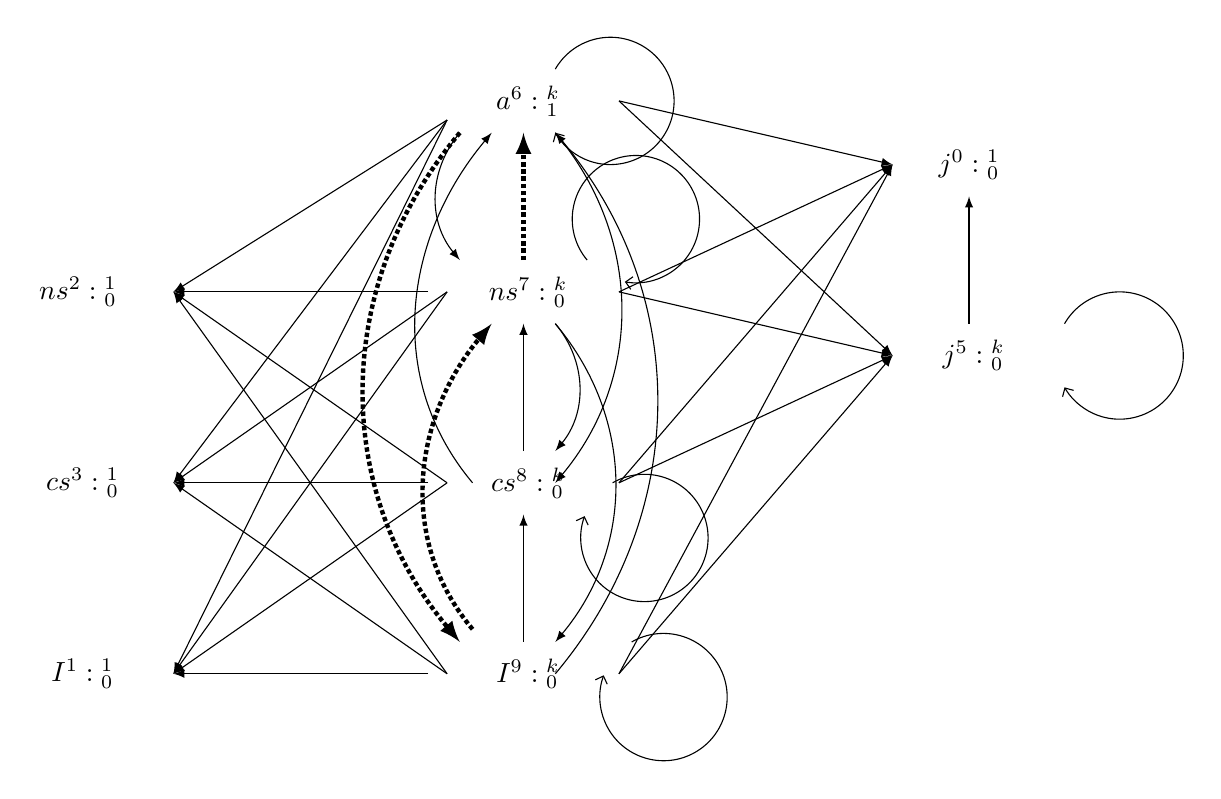
\begin{tikzpicture}[scale=\textwidth/15cm,samples=200]
    % Variables Initialization
     \draw[] (-7, 1) circle (0pt) node{{ $I^1: {}^1_{0}$}};
     \draw[] (-7, 7) circle (0pt) node{{$ns^2: {}^{1}_{0}$}};
     \draw[] (-7, 4) circle (0pt) node{{ $cs^3: {}^{1}_{0}$}};
     % Variables Inside the Loop
     \draw[] (0, 10) circle (0pt) node{{ $a^6: {}^{k}_{1}$}};
     \draw[] (0, 7) circle (0pt) node{{ $ns^7: {}^{k}_{0}$}};
     \draw[] (0, 4) circle (0pt) node{{ $cs^8: {}^{k}_{0}$}};
     \draw[] (0, 1) circle (0pt) node{{ $I^9: {}^{k}_{0}$}};
     % Counter Variables
     \draw[] (7, 9) circle (0pt) node {{$j^0: {}^{1}_{0}$}};
     \draw[] (7, 6) circle (0pt) node {{ $j^5: {}^{k}_{0}$}};
     %
     % Value Dependency Edges:
     \draw[  -latex,] (0, 1.5)  -- (0, 3.5) ;
     \draw[ ultra thick, -latex, densely dotted,] (0, 7.5)  -- (0, 9.5) ;
     \draw[  -Straight Barb] (1.4, 4) arc (120:-200:1);
     \draw[  -Straight Barb] (8.5, 6.5) arc (150:-150:1);
     \draw[  -Straight Barb] (1, 7.5) arc (220:-100:1);
     \draw[  -latex] (7, 6.5)  -- (7, 8.5) ;
     % Value Dependency Edges on Initial Values:
     \draw[  -latex,] (-1.5, 1)  -- (-5.5, 1) ;
     \draw[  -latex,] (-1.5, 4)  -- (-5.5, 4) ;
     \draw[  -latex,] (-1.5, 7)  -- (-5.5, 7) ;
     %
     \draw[ ultra thick, -latex, densely dotted,] (-1, 9.5)  to  [out=-130,in=130]  (-1, 1.5);
     \draw[ ultra thick, -latex, densely dotted,] (-0.8, 1.7)  to  [out=-230,in=230]  (-0.5, 6.5);
     % Value Dependency from cs8 -> a6
     \draw[  -latex, ] (-0.8, 4.0)  to  [out=-230,in=230]  (-0.5, 9.5);
     % Value Dependency from a6 -> I1
     \draw[  -latex,] (-1.2, 9.7)  -- (-5.5, 1);
     \draw[  -Straight Barb] (1.7, 1.5) arc (120:-200:1);
     % Control Dependency
     \draw[  -latex] (1.5, 7)  -- (5.8, 6) ;
     \draw[  -latex] (1.5, 4)  -- (5.8, 6) ;
     \draw[  -latex] (1.5, 1)  -- (5.8, 6) ;
     \draw[  -latex] (1.5, 10)  -- (5.8, 6) ;
     % Edges Produced by Transitivity by Control Dependency
     \draw[  -latex] (1.5, 7)  -- (5.8, 9) ;
     \draw[  -latex] (1.5, 4)  -- (5.8, 9) ;
     \draw[  -latex] (1.5, 1)  -- (5.8, 9) ;
     \draw[  -latex] (1.5, 10)  -- (5.8, 9) ;
     % Edges Produced by Transitivity from vertext a6 Dependency
     \draw[  -latex,] (-1.2, 9.7)  -- (-5.5, 4);
     \draw[  -latex,] (-1.2, 9.7)  -- (-5.5, 7);
     \draw[ -latex] (-1, 9.5)  to  [out=-130,in=130]  (-1, 7.5);
     \draw[ -latex] (0.5, 9.5)  to  [out=-50,in=50]  (0.5, 4);
     \draw[  -Straight Barb] (0.5, 10.5) arc (150:-150:1);
     % Edges Produced by Transitivity from vertext cs8 Dependency
     \draw[  -latex,] (-1.2, 4)  -- (-5.5, 1);
     \draw[  -latex,] (-1.2, 4)  -- (-5.5, 7);
     \draw[  -latex,] (0, 4.5)  -- (0, 6.5) ;
     % Edges Produced by Transitivity from vertext I9 Dependency
     \draw[  -latex,] (-1.2, 1)  -- (-5.5, 4);
     \draw[  -latex,] (-1.2, 1)  -- (-5.5, 7);
     \draw[  -latex,] (0.5, 1.0)  to  [out=50,in=-50]  (0.5, 9.5);
     % Edges Produced by Transitivity from vertext ns7 Dependency
     \draw[  -latex,] (-1.2, 7)  -- (-5.5, 1);
     \draw[  -latex,] (-1.2, 7)  -- (-5.5, 4);
     \draw[ -latex] (0.5, 6.5)  to  [out=-50,in=50]  (0.5, 1.5);
     \draw[ -latex] (0.5, 6.5)  to  [out=-50,in=50]  (0.5, 4.5);
     \end{tikzpicture}
     \caption{}
        \end{centering}
        \end{subfigure}
    \vspace{-0.4cm}
    \caption{(a) The simplified multiple rounds example (b) The estimated dependency graph from $\THESYSTEM$}
    \vspace{-0.5cm}
    \label{fig:multipleRounds}
\end{figure}
%
% %
\begin{example}[Linear Regression Algorithm with Gradient Decent Optimization]
\label{ex:linearregression}
    The linear regression algorithm with gradient decent Optimization works well 
    in our $\THESYSTEM$ as well.
            %   \[
            %   %
            %   \begin{array}{l}
            %   \kw{linearRegression(step, rate)} \triangleq \\
            %          \clabel{ a \leftarrow 0}^{0} ; \\
            %          \clabel{ c \leftarrow 0}^{1} ; \\
            %           \clabel{\assign{j}{\kw{step}} }^{2} ; \\
            %         %   \clabel{\assign{d}{10000000} }^{2} ; \\
            %           \ewhile ~ \clabel{j > 0}^{3} ~ \edo ~ \\
            %           \Big(
            %               \clabel{\assign{da}{\query(-2 * (\chi[1] - (\chi[0]\times a + c)) \times (\chi[0]))} }^{4}  ; \\
            %               \clabel{\assign{dc}{\query(-2 * (\chi[1] - (\chi[0]\times a + c)))} }^{5}  ; \\
            %               \clabel{\assign{a}{a - \kw{rate} * da} }^{6}  ; \\
            %               \clabel{\assign{c}{c - \kw{rate} * dc} }^{7}  ; \\
            %            \clabel{\assign{j}{j-1}}^{8} 
            %         %   \clabel{a \leftarrow x :: a}^{6} 
            %           \Big);
            %       \end{array}
            %   \]
              %
              %
                   %
\begin{figure}
\centering
\begin{subfigure}{0.45\textwidth}
    \centering
    {\small
        \[
        \begin{array}{l}
            \kw{linearRegressionGD(k, rate)} \triangleq \\
                   \clabel{ a \leftarrow 0}^{0} ; 
                   \clabel{ c \leftarrow 0}^{1} ; 
                    \clabel{\assign{j}{\kw{k}} }^{2} ; \\
                  %   \clabel{\assign{d}{10000000} }^{2} ; \\
                    \ewhile ~ \clabel{j > 0}^{3} ~ \edo ~ \\
                    \Big(
                        \clabel{\assign{da}{\query(-2 * (\chi[1] - (\chi[0]\times a + c)) \times (\chi[0]))} }^{4}  ; \\
                        \clabel{\assign{dc}{\query(-2 * (\chi[1] - (\chi[0]\times a + c)))} }^{5}  ; \\
                        \clabel{\assign{a}{a - \kw{rate} * da} }^{6}  ; 
                        \clabel{\assign{c}{c - \kw{rate} * dc} }^{7}  ; \\
                     \clabel{\assign{j}{j-1}}^{8} 
                  %   \clabel{a \leftarrow x :: a}^{6} 
                    \Big);
                \end{array}
        \]
        }
     \caption{}
        \end{subfigure}
      \begin{subfigure}{.45\textwidth}
          \begin{centering}
          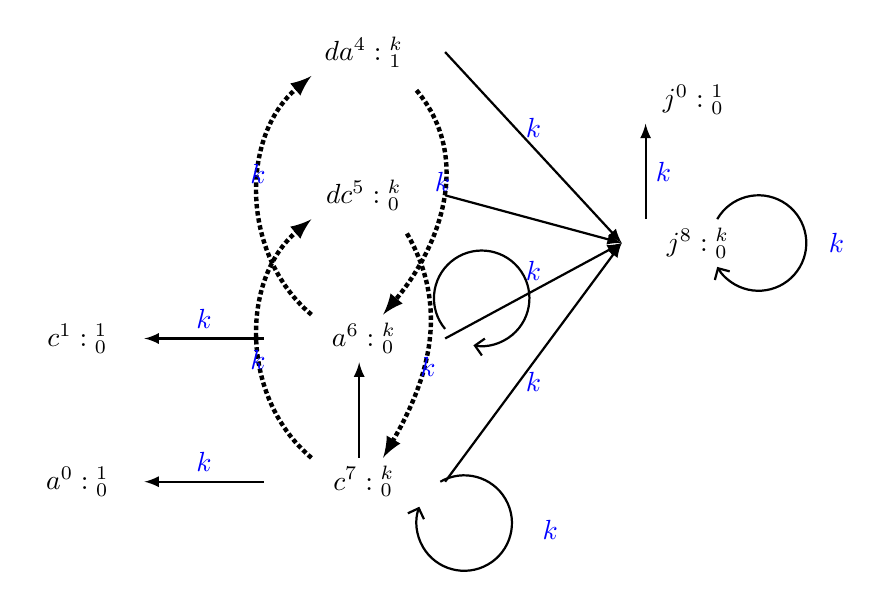
\begin{tikzpicture}[scale=\textwidth/20cm,samples=200]
    % Variables Initialization
    \draw[] (-6, 1) circle (0pt) node{{ $a^0: {}^1_{0}$}};
    \draw[] (-6, 4) circle (0pt) node{{ $c^1: {}^{1}_{0}$}};
    % Variables Inside the Loop
       \draw[] (0, 10) circle (0pt) node{{ $da^4: {}^{k}_{1}$}};
       \draw[] (0, 7) circle (0pt) node{{ $dc^5: {}^{k}_{0}$}};
       \draw[] (0, 4) circle (0pt) node{{ $a^6: {}^{k}_{0}$}};
       \draw[] (0, 1) circle (0pt) node{{ $c^7: {}^{k}_{0}$}};
       % Counter Variables
       \draw[] (7, 9) circle (0pt) node {{$j^0: {}^{1}_{0}$}};
       \draw[] (7, 6) circle (0pt) node {{ $j^8: {}^{k}_{0}$}};
       %
       % Value Dependency Edges:
       \draw[ thick, -latex,] (0, 1.5)  -- (0, 3.5) ;
       \draw[ thick, -Straight Barb] (1.8, 4.2) arc (220:-100:1);
       \draw[ thick, -Straight Barb] (7.5, 6.5) arc (150:-150:1);
       \draw[](10, 6) node[] {\highlight{$k$}} ;
       \draw[ thick, -Straight Barb] (1.7, 1.) arc (120:-200:1);
       \draw[](4, 0) node[] {\highlight{$k$}} ;
       \draw[ thick, -latex] (6, 6.5)  -- 
       node [right] {\highlight{$k$}}(6, 8.5) ;
       % Value Dependency Edges on Initial Values:
       \draw[ thick, -latex,] (-2, 1)  -- 
       node [above] {\highlight{$k$}}(-4.5, 1) ;
       \draw[ thick, -latex,] (-2, 4)  -- 
       node [above] {\highlight{$k$}}(-4.5, 4) ;
       %
       \draw[ ultra thick, -latex, densely dotted,] (-1, 1.5)  to  [out=-220,in=220]  
       node [below] {\highlight{$k$}}(-1, 6.5);
       \draw[ ultra thick, -latex, densely dotted,] (-1, 4.5)  to  [out=-220,in=220]  
       node [above] {\highlight{$k$}}(-1, 9.5);
       \draw[ ultra thick, -latex, densely dotted,]  (1, 6.2) to  [out=-60,in=60] 
       node [below] {\highlight{$k$}}(0.5, 1.5) ;
       \draw[ ultra thick, -latex, densely dotted,]  (1.2, 9.2)  to  [out=-50,in=50] 
       node [above] {\highlight{$k$}}(0.5, 4.5);
       % Control Dependency
      %  \draw[ thick,-latex] (1.5, 7)  -- (4, 9) ;
      %  \draw[ thick,-latex] (1.5, 4)  -- (4, 9) ;
       \draw[ thick,-latex] (1.8, 10)  -- 
       node [above] {\highlight{$k$}}(5.5, 6) ;
       \draw[ thick,-latex] (1.8, 7)  -- (5.5, 6) ;
       \draw[ thick,-latex] (1.8, 4)  -- 
       node [above] {\highlight{$k$}}(5.5, 6) ;
       \draw[ thick,-latex] (1.8, 1)  -- 
       node [below] {\highlight{$k$}}(5.5, 6) ;
       \end{tikzpicture}
       \caption{}
          \end{centering}
          \end{subfigure}
          %
        \begin{subfigure}{.8\textwidth}
            \begin{centering}
            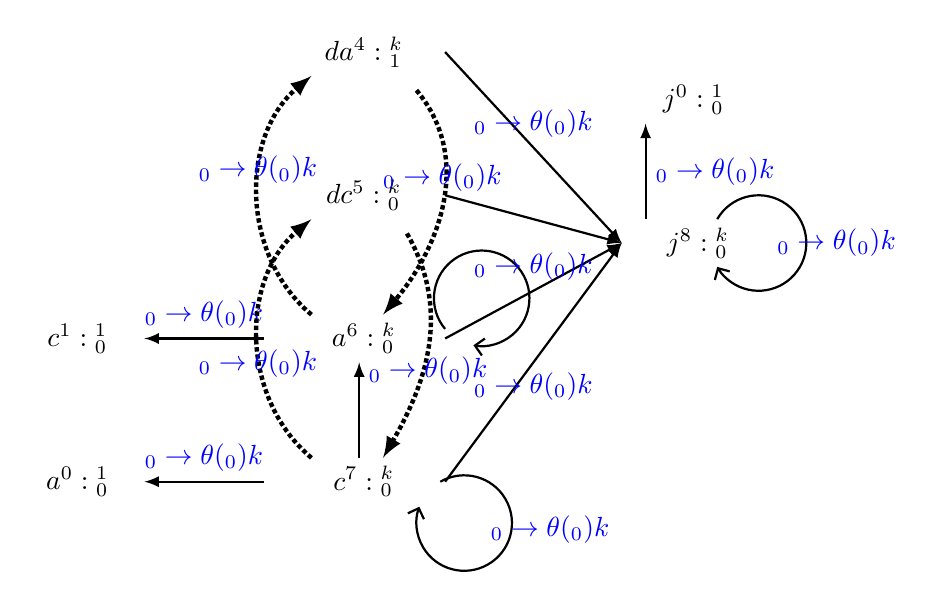
\begin{tikzpicture}[scale=\textwidth/20cm,samples=200]
      % Variables Initialization
      \draw[] (-6, 1) circle (0pt) node{{ $a^0: {}^1_{0}$}};
      \draw[] (-6, 4) circle (0pt) node{{ $c^1: {}^{1}_{0}$}};
      % Variables Inside the Loop
         \draw[] (0, 10) circle (0pt) node{{ $da^4: {}^{k}_{1}$}};
         \draw[] (0, 7) circle (0pt) node{{ $dc^5: {}^{k}_{0}$}};
         \draw[] (0, 4) circle (0pt) node{{ $a^6: {}^{k}_{0}$}};
         \draw[] (0, 1) circle (0pt) node{{ $c^7: {}^{k}_{0}$}};
         % Counter Variables
         \draw[] (7, 9) circle (0pt) node {{$j^0: {}^{1}_{0}$}};
         \draw[] (7, 6) circle (0pt) node {{ $j^8: {}^{k}_{0}$}};
         %
         % Value Dependency Edges:
         \draw[ thick, -latex,] (0, 1.5)  -- (0, 3.5) ;
         \draw[ thick, -Straight Barb] (1.8, 4.2) arc (220:-100:1);
         \draw[ thick, -Straight Barb] (7.5, 6.5) arc (150:-150:1);
         \draw[](10, 6) node[] {\highlight{$\trace_0 \to \env(\trace_0) k $}} ;
         \draw[ thick, -Straight Barb] (1.7, 1.) arc (120:-200:1);
         \draw[](4, 0) node[] {\highlight{$\trace_0 \to \env(\trace_0) k $}} ;
         \draw[ thick, -latex] (6, 6.5)  -- 
         node [right] {\highlight{$\trace_0 \to \env(\trace_0) k $}}(6, 8.5) ;
         % Value Dependency Edges on Initial Values:
         \draw[ thick, -latex,] (-2, 1)  -- 
         node [above] {\highlight{$\trace_0 \to \env(\trace_0) k $}}(-4.5, 1) ;
         \draw[ thick, -latex,] (-2, 4)  -- 
         node [above] {\highlight{$\trace_0 \to \env(\trace_0) k $}}(-4.5, 4) ;
         %
         \draw[ ultra thick, -latex, densely dotted,] (-1, 1.5)  to  [out=-220,in=220]  
         node [below] {\highlight{$\trace_0 \to \env(\trace_0) k $}}(-1, 6.5);
         \draw[ ultra thick, -latex, densely dotted,] (-1, 4.5)  to  [out=-220,in=220]  
         node [above] {\highlight{$\trace_0 \to \env(\trace_0) k $}}(-1, 9.5);
         \draw[ ultra thick, -latex, densely dotted,]  (1, 6.2) to  [out=-60,in=60] 
         node [below] {\highlight{$\trace_0 \to \env(\trace_0) k $}}(0.5, 1.5) ;
         \draw[ ultra thick, -latex, densely dotted,]  (1.2, 9.2)  to  [out=-50,in=50] 
         node [above] {\highlight{$\trace_0 \to \env(\trace_0) k $}}(0.5, 4.5);
         % Control Dependency
        %  \draw[ thick,-latex] (1.5, 7)  -- (4, 9) ;
        %  \draw[ thick,-latex] (1.5, 4)  -- (4, 9) ;
         \draw[ thick,-latex] (1.8, 10)  -- 
         node [above] {\highlight{$\trace_0 \to \env(\trace_0) k $}}(5.5, 6) ;
         \draw[ thick,-latex] (1.8, 7)  -- (5.5, 6) ;
         \draw[ thick,-latex] (1.8, 4)  -- 
         node [above] {\highlight{$\trace_0 \to \env(\trace_0) k $}}(5.5, 6) ;
         \draw[ thick,-latex] (1.8, 1)  -- 
         node [below] {\highlight{$\trace_0 \to \env(\trace_0) k $}}(5.5, 6) ;
         \end{tikzpicture}
         \caption{}
            \end{centering}
            \end{subfigure}
    \vspace{-0.5cm}
    \caption{(a) The linear regression algorithm 
    (b) The program-based dependency graph from $\THESYSTEM$
    (c) The execution-based dependency graph.}
    \vspace{-0.5cm}
    \label{fig:linear_regression}
\end{figure}
%
Analysis Result: $ \progA(\kw{linearRegressionGD(k, rate)}) = k$
\end{example} 
%
 
This linear regression algorithm 
% in order to
aims to
model a linear relationship between a dependent variable $y$,
% corresponding to the observed value in the column $\chi[1]$ in database, 
and an independent variable $x$, $y = a \times x + c$, specifically approximating the 
model parameter $a$ and $c$.
In order to have a good approximation on the model parameter 
$a$ and $c$, 
% corresponding to the observed value in the column $\chi[0]$ in database, 
it sends query to a training data set adaptively in every iteration.
This training data set contains two columns (can extend to higher dimensional data sets), first column is used as the observed value for the independent variable $x$,
second column is used as the observed label value for the dependent variable $y$.
This algorithm is written in our {\tt Query While} language in Figure~\ref{fig:linear_regression}(a) as $\kw{linearRegressionGD(k, rate)}$.
% taking the iteration number $\kw{step}$ 

This linear regression algorithm starts from initializing the linear model parameters and the counter variable,
and then goes into the training iterations.
In each iteration, it computes the differential value w.r.t. parameter
$a$ and $c$ respectively,
through requesting two queries, $\query(-2 * (\chi[1] - (\chi[0]\times a + c)) \times (\chi[0]))$ and 
$\query(-2 * (\chi[1] - (\chi[0]\times a + c)))$
at line 4 and 5.
Then, it uses these two differential values stored in variable $da$ and $dc$ to update the linear model parameters $a$ and $c$.
%
Its the program-based dependency graph is shown in Figure~\ref{fig:linear_regression}(b). Its execution-based dependency graph share the same graph, only needs to change the weight, $k$ into $w_k$ and $1$ for $w_1$ as we do in the previous example.
% We omit the detail of how to 
% generate this graph, which is similar to the generation procedure in 
% Example~\ref{alg:multiRound}.
In the execution-based dependency graph, there are multiple walks having the same longest query length.
For example, the walk $c^7 \to dc^6 : \to c^7 \to \cdots \to dc^6$ along the 
dotted arrows, where each vertex is visited $w_k(\trace_0)$ times for an initial trace $\trace_0$.
% By counting the total occurrence time of vertices with annotation $1$ in this walk, we have this program's adaptivity $k$.
There is actually other walks having the same query length $k$, the 
walk $a^7 \to da^6  \to a^7 \to \cdots \to da^6 $ along the 
dotted arrows, where each vertex is visited $w_k(\trace_0)$ times.
% the dotted path corresponds to a finite walk with the longest query length and its adaptivity on this walk is $k$.
But it doesn't affect the adaptivity for this program, which is still the maximal query length $w_k(\trace_0)$ with respect to initial trace $\trace_0$.
Also, $\THESYSTEM$, estimates the adaptivity $k$ for this example. Similarly as the multiple round example, we can show it is a tight bound.
%
% \begin{example}
[Multiple Rounds Odds Algorithm]
\label{ex:overapproximate}
The $\THESYSTEM$ comes across an over-approximation due to its path-insensitive nature. 
It occurs when the control flow can be decided in a particular way in front of conditional branches,
while the static analysis fails to witness. 

As in Figure~\ref{fig:overappr_example}(a), $\kw{multipleRoundsOdd}(k)$
is an example program with $1 + k$ adaptivity rounds and two paths while loop.
% we call it a multiple rounds odd iteration algorithm. 
In each iteration, 
the query $\query(\chi[x])$ in command $5$ is based on previous query results stored in $x$, which is similar to Example~\ref{ex:multipleRounds}.
The difference is that, only the query answers from the even iterations ($i = 0, 2, \cdots $) are 
% used to $b$. 
used in the query 
in command $7$, $\query(\chi[\ln(y)])$.
  Because the execution trace only updates 
%   $b$ using the query answers at odd iterations, so the answers from even iterations do not affect the queries at odd iterations. From the query-based dependency graph in Figure~\ref{fig:overappr_example}(b), we can see that there is no edge from queries at odd iterations (such as $q_1,q_3,q_5$) to queries at even iteration(such as $q_2,q_4$). The longest path is dashed with a length $3$.  However, {\THESYSTEM} fails to realize that odd iteration will always execute then branch and even iteration means else branch, so its dependency graph considers both branches for every iteration. In this sense, the dependency graph by {\THESYSTEM} is similar to the one in the multiple rounds strategy. We show the estimated graph in Figure~\ref{fig:overappr_example}(c). The estimated upper bound is then, $5$, instead of $3$. 
$x$ using the query answers in even iterations, so the answers from odd iterations do not affect the queries in even iterations. 
From the execution-based dependency graph in Figure~\ref{fig:overappr_example}(b), 
we can see that the weight for the vertex $y^5$ is 
$f_{k/2}$.
$f_{k/2} : \trace_0 \to (\env(\trace_0) k) / 2$, computes return the value of $k/2$ from input initial $\trace_0$.  
However, {\THESYSTEM} fails to realize that all the odd iterations only execute the first branch
and only even iterations execute the second branch. 
% its dependency 
So it considers both branches for every iteration when estimating the adaptivity. 
In this sense, the weight estimated for $y^5$ and $p^6$ are both 
$k$ as in Figure~\ref{fig:overappr_example}(c).
As a result, {\THESYSTEM}  estimates the longest walk from Figure~\ref{fig:overappr_example}(c) as
$y^5  \to x^7  \to y^5  \to \cdots \to x^7  $ with each vertex being visited $k$ times.
And the computed adaptivity  
% estimated from the program-based dependency graph graph from by finding the walk with the longest query length 
is $1 + 2 * k$, instead of $1 + k$. 
% We omitted the estimated graph, which is identical to the graph in Figure~\ref{fig:overappr_example}(b). 
%
{ \small
\begin{figure}
\centering
    \begin{subfigure}{0.33\textwidth}
\centering
\small{
    \[
    %
    \begin{array}{l}
        \kw{multipleRoundsOdd}(k) \triangleq \\
        \clabel{ \assign{j}{k}}^{0} ; 
        \clabel{ \assign{x}{\query(\chi[0])} }^{1} ; \\
            \ewhile ~ \clabel{j > 0}^{2} ~ \edo ~ 
            \Big(
             \clabel{\assign{j}{j-1}}^{3} ;\\
             \eif(\clabel{j \% 2 == 0}^{4}, \\
             \clabel{\assign{y}{\chi[x]}}^{5}, 
             \clabel{\assign{p}{\chi[x]}}^{6});\\                            
             \clabel{\assign{x}{\query(\chi(\ln(y)))} }^{7} \Big)
        \end{array}
    \]
}
 \caption{}
    \end{subfigure}
%
\begin{subfigure}{.31\textwidth}
    \begin{centering}
    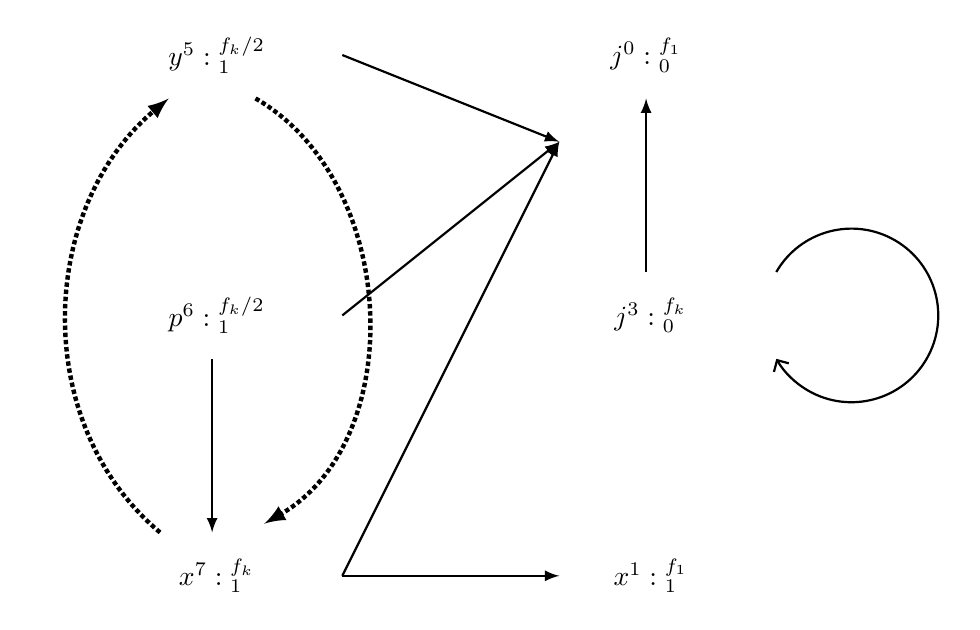
\begin{tikzpicture}[scale=\textwidth/11cm,samples=200]
% Variables Initialization
\draw[] (5, 1) circle (0pt) node{{ $x^1: {}^{f_1}_{1}$}};
% Variables Inside the Loop
 \draw[] (0, 7) circle (0pt) node{{ $y^5: {}^{f_k/2}_{1}$}};
 \draw[] (0, 4) circle (0pt) node{{ $p^6: {}^{f_k/2}_{1}$}};
 \draw[] (0, 1) circle (0pt) node{{ $x^7: {}^{f_k}_{1}$}};
 % Counter Variables
 \draw[] (5, 7) circle (0pt) node {{$j^0: {}^{f_1}_{0}$}};
 \draw[] (5, 4) circle (0pt) node {{ $j^3: {}^{f_k}_{0}$}};
 %
 % Value Dependency Edges:
 \draw[ thick, -latex,]  (0, 3.5) -- (0, 1.5) ;
%  \draw[ thick, -Straight Barb] (1, 4.2) arc (220:-100:1);
 \draw[ thick, -Straight Barb] (6.5, 4.5) arc (150:-150:1);
 \draw[ thick, -latex] (5, 4.5)  -- (5, 6.5) ;
%  \draw[ thick, -Straight Barb] (1., 1.5) arc (120:-200:1);
 % Value Dependency Edges on Initial Values:
 \draw[ thick, -latex,] (1.5, 1)  -- (4, 1) ;
 %
 \draw[ ultra thick, -latex, densely dotted,] (-0.6, 1.5)  to  [out=-220,in=220]  (-0.5, 6.5);
\draw[ ultra thick, -latex, densely dotted,]  (0.5, 6.5) to  [out=-30,in=30] (0.6, 1.6) ;
%  \draw[ ultra thick, -latex, densely dotted,]  (0.5, 10)  to  [out=-50,in=50] (0.5, 4);
 % Control Dependency
 \draw[ thick,-latex] (1.5, 7)  -- (4, 6) ;
 \draw[ thick,-latex] (1.5, 4)  -- (4, 6) ;
 \draw[ thick,-latex] (1.5, 1)  -- (4, 6) ;
%  \draw[ thick,-latex] (1.5, 10)  -- (4, 6) ;
 \end{tikzpicture}
 \caption{}
    \end{centering}
    \end{subfigure}
    \begin{subfigure}{.31\textwidth}
        \begin{centering}
        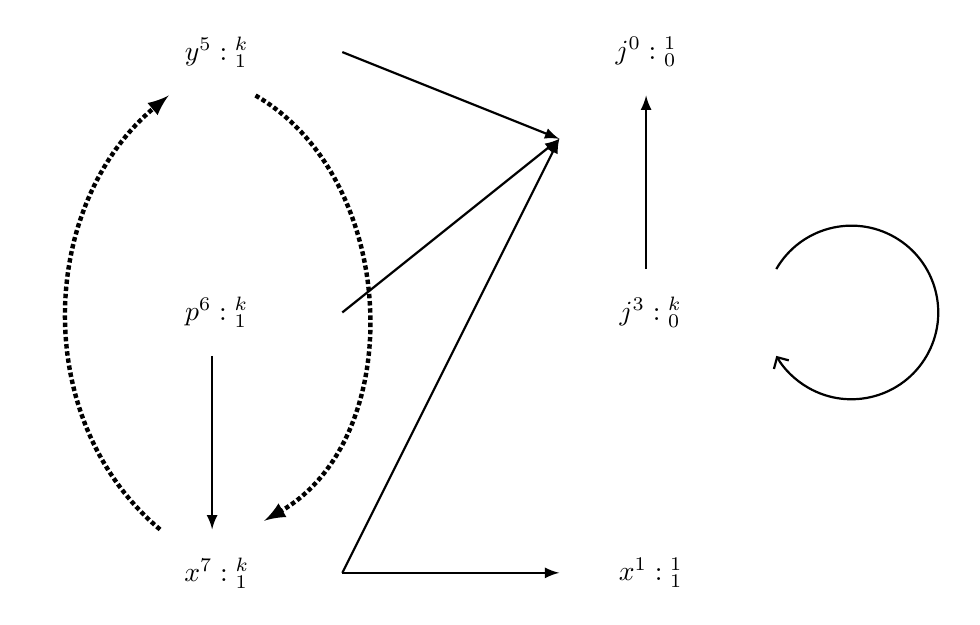
\begin{tikzpicture}[scale=\textwidth/11cm,samples=200]
    % Variables Initialization
    \draw[] (5, 1) circle (0pt) node{{ $x^1: {}^1_{1}$}};
    % Variables Inside the Loop
     \draw[] (0, 7) circle (0pt) node{{ $y^5: {}^{k}_{1}$}};
     \draw[] (0, 4) circle (0pt) node{{ ${p^6: {}^{k}_{1}}$}};
     \draw[] (0, 1) circle (0pt) node{{ ${x^7: {}^{k}_{1}}$}};
     % Counter Variables
     \draw[] (5, 7) circle (0pt) node {{$j^0: {}^{1}_{0}$}};
     \draw[] (5, 4) circle (0pt) node {{ $j^3: {}^{k}_{0}$}};
     %
% Value Dependency Edges:
 \draw[ thick, -latex,]  (0, 3.5) -- (0, 1.5) ;
%  \draw[ thick, -Straight Barb] (1, 4.2) arc (220:-100:1);
 \draw[ thick, -Straight Barb] (6.5, 4.5) arc (150:-150:1);
 \draw[ thick, -latex] (5, 4.5)  -- (5, 6.5) ;
%  \draw[ thick, -Straight Barb] (1., 1.5) arc (120:-200:1);
 % Value Dependency Edges on Initial Values:
 \draw[ thick, -latex,] (1.5, 1)  -- (4, 1) ;
 %
 \draw[ ultra thick, -latex, densely dotted,] (-0.6, 1.5)  to  [out=-220,in=220]  (-0.5, 6.5);
\draw[ ultra thick, -latex, densely dotted,]  (0.5, 6.5) to  [out=-30,in=30] (0.6, 1.6) ;
%  \draw[ ultra thick, -latex, densely dotted,]  (0.5, 10)  to  [out=-50,in=50] (0.5, 4);
 % Control Dependency
 \draw[ thick,-latex] (1.5, 7)  -- (4, 6) ;
 \draw[ thick,-latex] (1.5, 4)  -- (4, 6) ;
 \draw[ thick,-latex] (1.5, 1)  -- (4, 6) ;
%  \draw[ thick,-latex] (1.5, 10)  -- (4, 6) ;
     \end{tikzpicture}
     \caption{}
        \end{centering}
        \end{subfigure}
        \vspace{-0.4cm}
\caption{(a) The multiple rounds odd example 
(b) The execution-based dependency graph
(c) The program-based dependency graph graph from $\THESYSTEM$.}
    \label{fig:overappr_example}
    \vspace{-0.5cm}
\end{figure}
}
%
\end{example}
\begin{example}[Single Adaptivity Round Example]
    \label{ex:multiRoundsS}
    The program's adaptivity definition in our formal model,
    (in Definition~\ref{def:trace_adapt})
    comes across an over-approximation when capturing the program's intuitive adaptivity rounds.
    It results from the difference between its weight calculation and the \emph{variable may-dependency} definition.
    It occurs when the weight is computed over the traces different from the traces used in 
    witnessing the \emph{variable may-dependency} relation.
    
    The program $\kw{multiRoundsS(k)}$ in Figure~\ref{fig:multiRoundsS}(a) demonstrates this over-approximation.
    It is a variant of the multiple rounds strategy with input $k$.
    In each iteration, the query request $\clabel{\assign{p}{\query(\chi[y]+p)} }^{7}$ is based on value stored in $p$ and $y$ from previous iteration.
    Differ from Example~\ref{ex:multipleRounds},
    only the query answer from the $(k - 2)^{th}$ iteration is used in the query request, $\clabel{\assign{p}{\query(\chi[y]+p)} }^{7}$ of the next $(k - 1)^{th}$ iteration.
    % $\clabel{\assign{p}{\query(\chi[y]+p)} }^{7}$.
    In all the other iterations, $j \neq (k - 2)$, the if-control goes to the first branch
    % Because the execution will reset
    $p$'s value is reset by the constant $0$ in command $ \clabel{\assign{p}{0}}^{9}$.
    % in all the other iterations
    % at line $10$ after this query request.
    In this way, all the query answers stored in $p$ are erased and are not used
    in the query request at the next iteration, except the one at the $(k - 2)^{th}$ iteration.
    Intuitively, when $k \geq 2$, only the $\clabel{\assign{p}{\query(\chi[y]+p)} }^{7}$ in the $(k - 1)^{th}$ iteration
    depends on the query in $(k - 2)^{th}$ iteration and the \emph{adaptivity} round is $2$.
    When $k = 0$, the program does not go into the loop and there is no dependency between any query request.
    When $k = 1$, the program goes to the first branch in the first if-control with guard $\clabel{ k = 1}^{3}$.
    In this case, the second query request $ \clabel{ \assign{y}{\query(z)}}^{4}$ depends on the first one,
    $\clabel{\assign{z}{\query(0)} }^{1}$ and then the next query in the loop, $\clabel{\assign{p}{\query(\chi[y]+p)} }^{7}$ depends on the second one. Intuitively, the adaptivity is $3$.
    % In this sense, the intuitive \emph{adaptivity} rounds for this example is $2$. 
    However, our adaptivity definition fails to realize that there is only a dependency relation 
    between $p^7$ to itself at the $(k - 2)^{th}$ iteration.
    % but not in all the others. 
    As shown in the semantics-based dependency graph in Figure~\ref{fig:multiRoundsS}(b), 
    there is a cycle on $p^7$ representing the existence of the \emph{Variable May-Dependency} from $p^7$ on itself.
    % and the visiting times of labeled variable $p^7$ is 
    % $\lambda \trace_0 \st k$. 
    Weight of this vertex is $\lambda \trace_0 \st \env(\trace_0) k$,
    % The function $\lambda \trace_0 \st \env(\trace_0) k$ 
    which returns the evaluation times of the command $\clabel{\assign{p}{\query(\chi[y]+p)} }^{7}$ during the program execution under the initial trace $\trace_0$.
    % , which is expected to be equal to the loop iteration numbers, i.e., an initial value of input $k$ from the initial trace $\trace_0$.
    Since the command $\clabel{\assign{p}{\query(\chi[y]+p)} }^{7}$  will always be evaluated the same time as the loop iteration numbers, i.e. $k$,
    the weight function returns $\env(\trace_0) k$.
    However, $\env(\trace_0) k$ is the total number that this command is evaluated, rather than the number of the evaluations in which this command depends on other query requests.
    As a result, the walk with the longest query length 
    is
    $p^7 \to \cdots \to p^7 \to y^4 \to z^1 $ with the vertex $p^7$ visited $\env(\trace_0) k$ times, as the dotted arrows. 
    The adaptivity based on this walk
    is $\lambda \trace_0 \st \env(\trace_0) k + 2$,
    which is expected to be $0$ when $k = 0$ and $2$ when $k \geq 2$.
    %  instead of $\max\{0, 2, 3\}$. 
    % Though the $\THESYSTEM$ is able to give us $2 + k$, as an accurate bound w.r.t this definition.
    {
    \begin{figure}
    \centering
    %}
    \quad
    \begin{subfigure}{.8\textwidth}
    \begin{centering}
    {
    $ \begin{array}{l}
    \kw{multiRoundsS(k)} \triangleq \\
    \clabel{ \assign{j}{0}}^{0} ; 
    \clabel{\assign{z}{\query(0)} }^{1} ; 
    \clabel{\assign{p}{0} }^{2} ; \\
    \eif(\clabel{ k = 1}^{3},
    \clabel{ \assign{y}{\query(z)}}^{4},
    \clabel{\eskip}^5);\\
    \ewhile ~ \clabel{j \neq k}^{6} ~ \edo ~ \Big(
    \\
    \qquad \clabel{\assign{p}{\query(\chi[y]+p)} }^{7} ; \\
    \qquad 
    \eif(\clabel{ j \neq k - 2}^{8}, 
    \clabel{ \assign{p}{0}}^{9} ,
    \clabel{\eskip}^{10})  \\ 
    \qquad \clabel{\assign{j}{j + 1}}^{11} ; 
    \Big)
    \end{array}
    $ 
    }
    \caption{}
    \end{centering}
    \end{subfigure}
    \begin{subfigure}{.8\textwidth}
    \begin{centering}
    \begin{tikzpicture}[scale=\textwidth/15cm,samples=200]
    % Variables Initialization
    \draw[] (-5, 2) circle (0pt) node{{ $z^1: {}^{\lambda \trace_0 \st 1}$}};
    \draw[] (-5, 7) circle (0pt) node{{$p^2: {}^{\lambda \trace_0 \st 1}$}};
    \draw[] (-5, 4) circle (0pt) node{{ $y^4: {}^{\lambda \trace_0 \st 1}$}};
    % Variables Inside the Loop
    \draw[] (0, 6) circle (0pt) node{ $p^7: {}^{\lambda \trace_0 \st \env(\trace_0) k}$};
    \draw[] (0, 2) circle (0pt) node{ $p^{10}: {}^{\lambda \trace_0 \st \env(\trace_0) k}$};
    % Counter Variables
    \draw[] (5, 6) circle (0pt) node {$j^0: {}^{\lambda \trace_0 \st 1}$};
    \draw[] (5, 2) circle (0pt) node { $j^8: {}^{\lambda \trace_0 \st \env(\trace_0) k}$};
    %
    % Value Dependency Edges:
    \draw[ thick, -Straight Barb, densely dotted,] (0.8, 7) arc (220:-100:1);
    \draw[ -latex] (-1.5, 5.5) to [out=-130,in=130] (-1.5, 2);
    % Value Dependency Edges on Initial Values:
    \draw[ thick, -latex, densely dotted,] (-5, 3.5) -- (-5, 2.5) ;
    \draw[ -latex,] (-1.5, 5.5) -- (-4, 7) ;
    \draw[ thick, -latex, densely dotted,] (-1.5, 5.5) -- (-4, 4.7) ;
    \draw[ -latex,] (-1.5, 5.5) -- (-4, 2) ;
    %
    % Value Dependency For Control Variables:
    \draw[ -Straight Barb] (6.5, 2.5) arc (150:-150:1);
    % Control Dependency
    \draw[ -latex] (5, 2.5) -- (5, 5.5) ;
    \draw[ -latex] (1.2, 6) -- (3.5, 6) ;
    \draw[ -latex] (1.2, 6) -- (3.5, 2) ;
    \draw[ -latex] (1.5, 1.8) -- (3.5, 2) ; 
    % Edges Produced by Transitivity
    \draw[ -latex] (1.5, 1.8) -- (3.5, 6) ; 
    \end{tikzpicture}
    \caption{}
    \end{centering}
    \end{subfigure}
    \caption{(a) The loop example with single adaptivity rounds.
    (b) The corresponding semantics-based dependency graph.}
    \label{fig:multiRoundsS}
    \end{figure}
    }
    \end{example}

\subsection{Implementation Results}
We implemented $\THESYSTEM$ as a tool which takes a labeled command as input  
% labeled command 
and outputs an upper bound on the program adaptivity and on the number of query requests.
This implementation consists of an 
abstract control flow graph generation, weight estimation (as presented in Section~\ref{sec:alg_weightgen}),
edge estimation (as presented in Section~\ref{sec:alg_edgegen}) in Ocaml, 
and the adaptivity computation algorithm shown in Section~\ref{sec:alg_adaptcompute} in Python.
The OCaml program takes the labeled command as input and outputs the program-based dependency graph,
feeds into the python program and the python program provides the adaptivity upper bound and the query number as the final output.

We evaluated this implementation on $17$ example programs with the evaluation results shown  in Table~\ref{tb:imp}.
In this table,
the first column is the name of each program.
For each program $c$, the second column is its intuitive adaptivity rounds,
the third column is the $A(c)$ we defined through our formal semantic model above.
% in Section~\ref{sec:dep_adaptivity}.
In the third column, we use $k$ represent the weight function $w_k$ (in program's execution-based dependency graph) which return value of variable $k$ 
from an initial trace $\trace_0$, same for natural numbers.
The last column is the output of the $\THESYSTEM$ implementation, which consists of two expressions.
The first one is the upper bound for adaptivity and the second one is the 
upper bound for the total number of query requests in the program.

The first 3 programs we evaluated are $ \kw{twoRoundsComplete(k)}$, $ \kw{multipleRoundsComplete(k)}$, 
and the $\kw{linearRegressionGD(k, rate)}$ which we discussed in overview and above section.
% Section~\ref{sec:examples}.
% The same for the third programprograms in the table row 
For these examples, $A(c)$ 
% based dynamic analysis 
give the accurate adaptivity definition, 
simultaneously the $\THESYSTEM$ outputs the tight bounds for both of the adaptivity and query requesting number as expected.
% Look at 
% the $ \kw{linearRegressionGD(k)}$ which we discussed in Section~\ref{sec:examples}, the $\THESYSTEM$ outputs the accurate bound $k$ as expected.
But for the forth program $\kw{multipleRoundOdd(k)}$, $\THESYSTEM$ outputs an over-approximated upper bound $1 + 2*k$ for the $A(c)$, 
which is consistent with our expectation as discussed in Example~\ref{ex:multipleRoundSingle}. 
The fifth program is the evaluation results for the example in Example~\ref{ex:multipleRoundSingle}, where $\THESYSTEM$ outputs
the tight bound for $A(c)$ but $A(c)$ is a loose definition of the program's actual adaptivity rounds.
%
The programs in the table from  $\kw{seq()}$ to $ \kw{nestedWhileMultiPathMultiVarRecAcross(k)}$ are 
designed for testing the programs under different possible situitions.
These programs contain control dependency, data value dependency,
the nested while, dependency through multiple variables, dependency across nested loops, and so on. 
Overall for these examples, our system gives both the accurate adaptivity definition and 
adaptivity upper bound simultaneously through the dynamic analysis and 
static analysis.
The full programs are defined below from Example~\ref{ex:twoRoundsComplete} to Example~\ref{ex:nestedWhileMultiVarRecAcross}.
%
\begin {table}[H]
        \vspace{-0.3cm}
    \caption{Experimental results of {\THESYSTEM} implementation}
        \label{tb:imp}
        \begin{center}
        \vspace{-0.3cm}
{\footnotesize
        \begin{tabular}{ c c c c}
         Program $c$ & adaptivity rounds & $A(c)$ & $\THESYSTEM$ \\ 
         $ \kw{twoRoundsComplete(k)}$ & $2$ & $2$ & $2$, $k$ \\
         $ \kw{multipleRoundsComplete(k)}$ & $k$ & $k$ & $k$, $k$  \\
         $\kw{linearRegressionGD(k, rate)}$ & $k$ & $k$ & $k$, $2 * k$  \\
         $ \kw{multipleRoundsOdd(k)}$ & $1 + k$ & $1 + k$ & $1 + 2*k$, $1 + 2*k$  \\
         $ \kw{multipleRoundsSingle(k)}$ & $2$ & $2 + k$ & $2 + k$ , $2 + k$  \\
         $\kw{seq()}$ & $4$ & $4$ & $4$, $4$  \\ 
         $\kw{seqMultiVar()}$ & $4$ & $4$ & $4$, $4$ \\  
         $ \kw{ifValueDependency}$ & $3$ & $3$ & $3$, $3$ \\
         $\kw{ifControlDependency()}$ & $3$ & $3$ & $3$, $3$  \\
         $ \kw{whileRec(k)}$ & $1+k$ & $1+k$ & $1+k$  \\
        %  $ \kw{whileMultiplePath(k)}$ & $1 + k$ & $1 + k$ & $1 + 2 * k$, $1 + 2 * k$  \\
         $ \kw{whileMultipleVar(k)}$ & $1 + 2*k$ & $1 + 2*k$ & $1 + 2*k$, $2 + 3 * k$  \\
         $ \kw{whileValueControlDependency(k)}$ & $1 + 2*k$ & $1 + 2*k$ & $1 + 2 * k$, $2 + 2 * k$  \\
         $ \kw{whileMultiplePathValueControlDependency(k)}$ & $2 + k$ & $2 + k$  & $2 + k$, $1 + 2 * k$   \\
         $ \kw{nestWhileValueDependency(k)}$ & $2 + k^2$ & $2 + k^2$  & $2 + k^2$, $1 + k + k^2$   \\
         $ \kw{nestedWhileRecAcross(k)}$ & $1 + 2*k$ & $1 + 2*k$ & $1 + 2*k$,  $1 + k + k^2$   \\
         $ \kw{nestedWhileMultiVarRecAcross(k)}$ & $1 + k + k^2$ & $1 + k + k^2$  & $1 + k + k^2$,  $2 + k + k^2$  \\
         $ \kw{nestedWhileMultiPathMultiVarRecAcross(k)}$ & $1 + k + k^2$ & $1 + k + k^2$  & $1 + k + k^2$,  $2 + k + k^2$  \\
        \end{tabular}
}        
\end{center}
\end{table}
        %
\begin{example}[Complete Two Round Algorithm]
        \label{ex:twoRoundsComplete}
        \[
        %
            \kw{twoRoundsComplete(k)} \triangleq
        \begin{array}{l}
               \clabel{ a \leftarrow []}^{1} ; \\
                \clabel{\assign{j}{k} }^{2} ; \\
                \ewhile ~ \clabel{j > 0}^{3} ~ \edo ~ \\
                \Big(
                 \clabel{\assign{x}{\query(\chi[k - j]\cdot \chi[k])} }^{4}  ; \\
                 \clabel{\assign{j}{j-1}}^{5} ;\\
                \clabel{a \leftarrow x :: a}^{6}       \Big);\\
                \clabel{l \leftarrow (\mathrm{sign}\big (\sum_{i\in [k]} \chi[i]\times\ln\frac{1+a[i]}{1-a[i]} \big ))}^{7}\\
            \end{array}
        \]
        %
        \begin{algorithm}
        \footnotesize
        \caption{A two-round analyst strategy for random data (The example in  \cite{dwork2015preserving})}
        \label{alg:twoRound}
        \begin{algorithmic}
        \REQUIRE Mechanism $\mathcal{M}$ with a hidden data set $D \in \{-1,+1\}^{n\times (k+1)} \subset \dbdom$.
        \STATE  {\bf for}\ $j\in [k]$\ {\bf do}.  
        \STATE \qquad {\bf define} $q_j(d)=d(j)\cdot d(k)$ where $d \in \{D(i) ~|~ i = 0, \cdots, n\} \subseteq \{-1,+1\}^{k+1}$.
        \STATE \qquad {\bf let} $a_j=\mathcal{M}(q_j)$ 
        \STATE \qquad \COMMENT{In the line above, $\mathcal{M}$ computes approx. the exp. value  of $q_j$ over $D$. So, $a_j\in [-1,+1]$.}
        \STATE {\bf define} $q_{k}(d)= d(k) \cdot \mathrm{sign}\big (\sum_{i\in [k]} x(i) \cdot \ln\frac{1+a_i}{1-a_i} \big )$ where $x\in \{-1,+1\}^{k+1}$.
        \STATE\COMMENT{In the line above,  $\mathrm{sign}(y)=\left \{ \begin{array}{lr} +1 & \mathrm{if}\ y\geq 0\\ -1 &\mathrm{otherwise} \end{array} \right . $.}
        \STATE {\bf let} $a_{k+1}=\mathcal{M}(q_{k+1})$
        \STATE\COMMENT{In the line above,  $\mathcal{M}$ computes approx. the exp. value  of $q_{k+1}$ over $X$. So, $a_{k+1}\in [-1,+1]$.}
        \RETURN $a_{k+1}$.
        \ENSURE $a_{k+1}\in [-1,+1]$
            % \ENSURE 
        \end{algorithmic}
        \end{algorithm}
        %
    %
        \end{example}
    
    \begin{example}[Complete Multiple Round Algorithm]
    %
    \begin{algorithm}
    \footnotesize
    \caption{A multi-round analyst strategy for random data base \cite{dwork2015preserving}}
    \label{alg:multiRound}
    \begin{algorithmic}
    \REQUIRE Mechanism $\mathcal{M}$ with a hidden state $X\in [N]^{n}$ sampled u.a.r., control set size $c$
    \STATE Define control dataset $C = \{0,1, \cdots, c - 1\}$
    \STATE Initialize $Nscore(i) = 0$ for $i \in [N]$, $I = \emptyset$ and $Cscore(C(i)) = 0$ for $i \in [c]$
    \STATE  {\bf for}\ $j\in [k]$\ {\bf do} 
    \STATE \qquad {\bf let} $p=\uniform(0,1)$ 
    \STATE \qquad {\bf define} $q (x) = \bernoulli ( p )$ .
    \STATE \qquad {\bf define} $qc (x) = \bernoulli ( p )$ .
    \STATE \qquad {\bf let} $a = \mathcal{M}(q)$ 
    \STATE \qquad {\bf for}\ $i \in [N]$\ {\bf do}
    \STATE \qquad \qquad $Nscore(i) = Nscore(i) + (a - p)*(q (i) - p)$ if $i \notin I$
    \STATE \qquad {\bf for}\ $i \in [c]$\ {\bf do}
    \STATE \qquad \qquad $Cscore(C(i)) = Cscore(C(i)) + (a - p)*(qc (i) - p)$
    \STATE \qquad {\bf let} $I = \{i | i\in [N] \land Nscore(i) > \max(Cscore)\}$
    \STATE \qquad {\bf let} $D = D \setminus I$ 
    \RETURN $D$.
    \end{algorithmic}
    \end{algorithm}
    %
    {\small
    \begin{figure}
    %     \begin{subfigure}{0.3\textwidth}
    %     \begin{centering}
    %     $
    % %     \begin{array}{l}
    % %     %  \left[j \leftarrow 0 \right]^1 ; \\
    % %     \clabel{I \leftarrow [] }^1; \\
    % %     \clabel{\assign{ns}{0} }^{2}; \\
    % %      \clabel{\assign{cs}{0} }^{3}; \\
    % %     \eloop ~ [3]^{4} ~  
    % %     \ ~ \edo ~ \\ 
    % %     \quad \clabel{a \leftarrow q(f( I)) }^{5}; \\
    % %     \quad \clabel{\assign{ns}{update\_nscore(a)}; }^{6}\\
    % %     \quad \clabel{\assign{cs}{update\_cscore(a)}; }^{7}\\
    % %     \quad \clabel{I \leftarrow \mathsf{update} ( I, ns, cs)  }^{8}
    % % \end{array}
    % % \kw{multipleRoundsSimp(k, c)} \triangleq
    % % \begin{array}{l}
    % %      \left[j \leftarrow k \right]^1 ; \\
    % %     \left[I \leftarrow [] \right]^2; \\
    % %     \ewhile ~ \clabel{j > 0}^{3} ~ \edo ~ \\
    % %     \Big(
    % %     \clabel{\assign{j}{j-1}}^{4} ;\\
    % %     \left[p \leftarrow c \right]^5; \\
    % %     \left[ a \leftarrow \query (\chi[I]) \right]^6;\\
    % %     \left[I \leftarrow \mathrel{\mathsf{update}} ( {I}, (a, p))  \right]^7
    % %     \Big) 
    % % \end{array}
    %     $
    %     \caption{}
    %     \end{centering}
    %     \end{subfigure}
        \begin{subfigure}{0.8\textwidth}
        \begin{centering}
        $
    \kw{multipleRoundsComplete(k, c, N)} \triangleq
    \begin{array}{l}
        \clabel{\assign{j}{N}}^0 ; 
         \clabel{\assign{cs}{0}}^1; 
         \clabel{\assign{ns}{0}}^2;
         \clabel{\assign{I}{0}}^3; 
         \clabel{\assign{w}{k}}^{4} ;\\
         \ewhile ~ \clabel{j > 0}^{5} ~ \edo ~ \\
         \Big(
         \clabel{\assign{j}{j-1}}^{6} ;
         \clabel{\assign{cs}{0 + cs}}^7; 
         \clabel{\assign{ns}{0 + ns}}^8
         \Big); \\
    
         \ewhile ~ \clabel{w > 0}^{9} ~ \edo ~ \\
        \Big(
        \clabel{\assign{w}{w-1}}^{10} ;
        \left[p \leftarrow c \right]^{11}; 
        \left[q \leftarrow c \right]^{12}; 
        \left[ a \leftarrow \query (\chi[I]) \right]^{13};\\
        \clabel{\assign{i}{N}}^{14} ; 
        \ewhile ~ \clabel{i > 0}^{15} ~ \edo ~ \\
        \Big(
        \clabel{\assign{i}{i-1}}^{16} ;
        \clabel{\assign{cs(i)}{cs(i) + (a - p) * (q - p)}}^{17}; \\
        \eif (\clabel{ I < i}^{18}, \clabel{\assign{ns(i)}{{ns(i) + (a - p) * (q - p)}}}^{19},
        \clabel{\assign{ns}{ns(i)}}^{20}    )
        \Big); \\
        \clabel{\assign{i2}{N}}^{21} ; \\
        \ewhile ~ \clabel{i2 > 0}^{22} ~ \edo ~ \\
        \Big(
        \clabel{\assign{i2}{i2-1}}^{23} ;
        \eif (\clabel{ns(i2) > \kw{max}(cs)}^{24}, 
        \clabel{\assign{I}{i + I}}^{25},
        \clabel{\assign{I}{I}}^{26})
        \Big)
        \Big) 
    \end{array}
       $
       \caption{}
        \end{centering}
        \end{subfigure}
        \vspace{-0.3cm}
        \caption{(a) The labeled program implementing the multiple round algorithm (b)The same program in the SSA version}
        \vspace{-0.5cm}
        \label{fig:multiround_complete}
        \end{figure}
    }
    %
    \end{example}
      We have seen the two round algorithm above. We show the multiple-round algorithm, which is an advanced algorithm.
    
    
    \begin{example}[Gradient Decent Optimization Algorithm]
        This example is the gradient decent algorithm example is a generalization of the linear regression on a higher degree data relation.
        It uses gradient decent algorithm to minimize 
        the mean square loss function
        for a two-degree relation
         $y = a_1 \times x_1^2 + a_2 \times x_2 + c$
        on the dataset of two feature columns and one indicator column.
                  \[
                  %
                  \begin{array}{l}
                  \kw{gradientDecent(step, rate, t, n)} \triangleq \\
                         \clabel{ a_1 \leftarrow 0}^{0} ; \\
                         \clabel{ a_2 \leftarrow 0}^{1} ; \\
                         \clabel{ c \leftarrow 0}^{2} ; \\
                          \clabel{\assign{j}{\kw{step}} }^{3} ; \\
                        %   \clabel{\assign{d}{10000000} }^{2} ; \\
                          \ewhile ~ \clabel{j > 0}^{4} ~ \edo ~ \\
                          \Big(
                              \clabel{\assign{da1}{\query(-2 * (\chi[2] - (\chi[0]^2 \times a_1 + \chi[1] \times a_2 + c)) \times (\chi[0]))} }^{5}  ; \\
                              \clabel{\assign{da2}{\query(-2 * (\chi[2] - (\chi[0]^2 \times a_1 + \chi[1] \times a_2 + c)) \times (\chi[1]))} }^{6}  ; \\                      \clabel{\assign{dc}{\query(-2 * (\chi[2] - (\chi[0]^2 \times a_1 + \chi[1] \times a_2 + c)))} }^{5}  ; \\
                              \clabel{\assign{a_1}{a_1 - \kw{rate} * da1} }^{7}  ; \\
                              \clabel{\assign{a_2}{a_2 - \kw{rate} * da2} }^{8}  ; \\
                              \clabel{\assign{c}{c - \kw{rate} * dc} }^{9}  ; \\
                           \clabel{\assign{j}{j-1}}^{10} 
                        %   \clabel{a \leftarrow x :: a}^{6} 
                          \Big);
                      \end{array}
                  \]
                  %
                  %
        It is easy to see, this approach can be generalized to the regression of a variety of 
        relations in machine learning area.
                       %
                  \end{example}
         
           
                  
                  
        \begin{example}[convex optimization Algorithm]
                  \[
                  %
                  \begin{array}{l}
                  \kw{gradientDecent(step, rate, t, n)} \triangleq \\
                         \clabel{ a \leftarrow []}^{0} ; \\
                          \clabel{\assign{j}{\kw{step}} }^{1} ; \\
                        %   \clabel{\assign{d}{10000000} }^{2} ; \\
                          \ewhile ~ \clabel{j > 0 \land d < t}^{3} ~ \edo ~ \\
                          \Big(
                              \clabel{\assign{d}{\query(2 * (\chi[1] - (\chi[0]\times x )) * (-\chi[0]))} }^{4}  ; \\
                              \clabel{\assign{x}{x - \kw{rate} * d} }^{4}  ; \\
                           \clabel{\assign{j}{j-1}}^{5} ;\\
                          \clabel{a \leftarrow x :: a}^{6} 
                          \Big);
                      \end{array}
                  \]
                  %
                  %
                       %
                  \end{example}    
    
    \begin{example}[Sequence with Single Variable Linear Data Value Dependency]
        \label{ex:seq}
        %
        %
        \[
        %
            \kw{seq()} \triangleq 
        \begin{array}{l} 
               \clabel{ \assign{x}{\chi[0]}}^{0} ; \\
                \clabel{\assign{y}{\chi[x + 1]} }^{1} ; \\
                \clabel{\assign{z}{\chi[y + 1]}}^{2}; \\
                 \clabel{\assign{w}{\chi[z + 1]} }^{3}
            \end{array}
        \]
        Analysis Result: $ \progA( \kw{seq()}) = 4$
        \end{example}
    %
    \begin{example}[Sequence with Multiple Variables Data Value Dependency]
        \label{ex:seqMultiVar}
        %
        %
        \[
        %
            \kw{seqMultiVar()} \triangleq 
        \begin{array}{l} 
               \clabel{ \assign{x}{\chi[0]}}^{0} ; \\
                \clabel{\assign{y}{\chi[x + 1]} }^{1} ; \\
                \clabel{\assign{z}{\chi[y + x]}}^{2}; \\
                 \clabel{\assign{w}{\chi[z + 1] \cdot \chi[y]} }^{3}
            \end{array}
        \]
        Analysis Result: $ \progA(\kw{seqMultiVar()}) = 4$
    \end{example}
    %
        \begin{example}[If with Data-Value Dependency Separated]
            \label{ex:ifValueDependency}
            %
            %
            \[
            %
            \kw{ifValueDependency}(k) \triangleq 
            \begin{array}{l}
               \quad \clabel{ \assign{z}{\query(\chi[0])}}^{0} ; \\
               \quad \clabel{\assign{x}{k / 2} }^{1} ; \\
               \quad \eif(\clabel{x < 0}^2, \\
               \quad \clabel{\assign{y}{\query(\chi[z])}}^{3}, \\ 
               \quad \clabel{\assign{y}{\query(\chi[0])}}^{4})
                \end{array}
            \]
            Analysis Result: $ \progA( \kw{ifControlDependency()}) = 3$
        \end{example}
    
            \begin{example}[If with Data-Control Dependency Overlapped]
                \label{ex:ifValueDependency}
                %
                %
                \[
                %
                \kw{ifControlDependency()} \triangleq 
                \begin{array}{l}
                    \clabel{ \assign{z}{\query(\chi[0])}}^{0} ; \\
                    \clabel{\assign{x}{\query(\chi[z])} }^{1} ; \\
                    \eif(\clabel{x < 0}^{2}, 
                    \clabel{\assign{y}{\query(\chi[0] + \chi[1])}}^{3}, 
                    \clabel{\assign{y}\query{(\chi[0])}}^{4})
                \end{array}
                \]
                %
                Analysis Result: $ \progA( \kw{ifControlDependency()}) = 3$
                \end{example}
    
    
                \begin{example}[Simple While with Recursive Data-Value Dependency]
                    \label{ex:ifValueDependency}
                    %
                    %
                    \[
                    %
                    \kw{whileRec}(k) \triangleq
                    \begin{array}{l}
                        \clabel{ \assign{j}{k} }^{0} ; \\
                        \clabel{ \assign{a}{\query(\chi[0])} }^{1} ; \\
                            \ewhile ~ \clabel{j > 0}^{2} ~ \edo ~ \\
                            \Big(
                             \clabel{\assign{x}{\query(\chi[a]) }}^{3}  ; \\
                             \clabel{\assign{a}{x + a}}^{4} ;\\
                            \clabel{\assign{j}{j-1}}^{5}       \Big)
                        \end{array}
                    \]
                    Analysis Results: $ \progA(\kw{whileRec}(k)) = 1 + k$
                \end{example}
    %
            \begin{example}[Simple While with Multi-Path Data-Value Dependency]
                \label{ex:whileMultiplePath}
                %
            %
            \[
            %
            \kw{whileMultiplePath}(k) \triangleq 
            \begin{array}{l}
                \clabel{ \assign{j}{k}}^{0} ; \\
                \clabel{ \assign{x}{\query(\chi[0])} }^{1} ; \\
                    \ewhile ~ \clabel{j > 0}^{2} ~ \edo ~ \\
                    \Big(
                     \clabel{\assign{j}{j-1}}^{3} ;\\
                     \eif(\clabel{j \% 2 == 0}^{4}, 
                     \clabel{\assign{y}{\chi[x]}}^{5}, 
                     \clabel{\assign{w}{\chi[x]}}^{6});\\                            
                     \clabel{\assign{x}{\query(\chi(\ln(y)))} }^{7} \Big)
                \end{array}
            \]
            Analysis Results: $ \progA(\kw{whileMultiplePath}(k)) = 1 + 2 * k $ --> Over-Approximated
        \end{example}
    %
            \begin{example}[Simple While with Recursive Multiple-Variable Data-Value Dependency]
                \label{ex:whileMultipleVar}
                \[
                %
                \kw{whileMultipleVar}(k) \triangleq 
                \begin{array}{l}
                \clabel{\assign{j}{k} }^{0} ; \\
                \clabel{ \assign{x}{\query(\chi[0])}}^{1} ; \\
                    \clabel{ \assign{y}{\query(\chi[1])}}^{2} ; \\
                        \ewhile ~ \clabel{j > 0}^{3} ~ \edo ~ \\
                        \Big(
                         \clabel{\assign{j}{j-1}}^{4} ;\\
                         \clabel{\assign{z}{\query(\chi(x + \ln(y)))} }^{5}  ; \\
                         \clabel{ \assign{x}{\query(\chi[z])}}^{6} ; \\
                         \clabel{ \assign{y}{\query(\chi[z])}}^{7} 
                        \Big)
                    \end{array}
                \]
                Analysis Results: $ \progA(\kw{whileMultipleVar}(k)) = 1 + 2 * k $
            \end{example}
                %
                %
                \begin{example}[Simple While with Data-Value and Data-Control Dependency]
                    \label{ex:whileValueControlDependency}
                    %
                    \[
                    \kw{whileValueControlDependency}() \triangleq
                    \begin{array}{l}
                        \clabel{ \assign{x}{\query(\chi[0])} }^{0} ; \\
                        \clabel{ \assign{z}{\query(\chi[0])} }^{1} ; \\
                            \ewhile ~ \clabel{x > 0}^{2} ~ \edo ~ \\
                            \Big(
                            \clabel{\assign{x}{\query(\chi(z))} }^{3}  ; \\
                            \clabel{\assign{z}{\query(\chi(x))}}^{4}
                          \Big)
                        \end{array}
                    \]
                    Analysis Results: $ \progA(\kw{whileValueControlDependency}(k)) = 1 + 2 * k $
                \end{example}
    %
                \begin{example}[Simple While with MultiplePath Data-Value and Data-Control Dependency]
                    \label{ex:whileMultiplePathValueControlDependency}
                    %
                    \[
                        %
                        \begin{array}{l}
                        \kw{whileMultiplePathValueControlDependency}(k) \triangleq\\
                            \clabel{ \assign{x}{\query(k)}}^{0} ; \\
                            \clabel{\assign{y}{0} }^{1} ; \\
                                \ewhile ~ \clabel{x > 0}^{2} ~ \edo ~ \\
                                \Big(
                                 \eif(\clabel{y > 0}^{3}, 
                                 \clabel{\assign{y}{\query(\chi[12])}}^{4}, 
                                 \clabel{\assign{w}{\query(\chi[9])}}^{5});                            
                                 \\
                                 \clabel{\assign{x}{x-1}}^{6}\Big);\\
                                 \clabel{\assign{y}{\query(\chi(\ln(y)))} }^{7} 
                            \end{array}
                        \]
                        Analysis Results: $ \progA(\kw{whileMultiplePathValueControlDependency}(k)) = 2 + k $
                    \end{example}
                                    %
                    \begin{example}[Nested While with Recursive Data-Value Dependency]
                        \label{ex:nestWhileValueDependency}
                        %
                        %
                        \[
                        %
                        \kw{nestWhileValueDependency}(k) \triangleq 
                        \begin{array}{l}
                            \clabel{ \assign{i}{k} }^{0} ; \\
                            \clabel{\assign{x}{\query(\chi[0])}}^{1} ; \\
                                \ewhile ~ \clabel{i > 0}^{2} ~ \edo ~ \\
                                \Big(
                                 \clabel{\assign{i}{i-1}}^{3} ;\\
                                 \clabel{\assign{j}{k}}^{4} ;\\
                                 \clabel{\assign{y}{\query(\chi(\ln(x)))} }^{5}  ; \\
                                 \ewhile ~ \clabel{j > 0}^{6} ~ \edo ~ \\
                                 \Big(
                                  \clabel{\assign{j}{j-1}}^{7};\\
                                  \clabel{\assign{x}{\query(\chi(\ln(x)))} }^{8}
                                  \Big) \Big)
                            \end{array}
                        \]
                        Analysis Results: $ \progA(\kw{nestWhileValueDependency}(k)) = 2 + k^2 $
                    \end{example}
    
                        \begin{example}[Nested While with Nested Recursive Data-Value Dependency Across Outer and Inner Loop]
                            \label{ex:nestedWhileRecAcross}
                            %
                            %
                            \[
                            %
                                \kw{nestedWhileRecAcross}(k) \triangleq 
                            \begin{array}{l}
                                \clabel{ \assign{i}{k} }^{0} ; \\
                                \clabel{\assign{x}{\query(\chi[0])}}^{1} ; \\
                                    \ewhile ~ \clabel{i > 0}^{2} ~ \edo ~ \\
                                    \Big(
                                     \clabel{\assign{i}{i-1}}^{3} ;\\
                                     \clabel{\assign{j}{k}}^{4} ;\\
                                     \ewhile ~ \clabel{j > 0}^{5} ~ \edo ~ \\
                                     \Big(
                                      \clabel{\assign{j}{j-1}}^{6};\\
                                      \clabel{\assign{y}{\query(\chi(x) + \chi(1))} }^{7}
                                      \Big); \\
                                     \clabel{\assign{x}{\query(\chi(\ln(y)))} }^{8}
                                      \Big)
                                \end{array}
                            \]
                            Analysis Results: $ \progA(\kw{nestedWhileRecAcross}(k)) = 1 + 2 * k $
                        \end{example}
                    %
                
                            \begin{example}[Nested While with Nested Recursive Multiple Variable 
                                Data-Value Dependency Across Outer and Inner Loop]
                                \label{ex:nestedWhileMultiVarRecAcross}
                                %
                                \[
                                %
                                \kw{nestedWhileMultiVarRecAcross}(k) \triangleq 
                                \begin{array}{l}
                                    \clabel{\assign{i}{k} }^{0} ; \\
                                    \clabel{ \assign{x}{\query(\chi[0])}}^{1} ; \\
                                    \clabel{ \assign{y}{\query(\chi[1])}}^{2} ; \\
                                        \ewhile ~ \clabel{i > 0}^{3} ~ \edo ~ \\
                                        \Big(
                                         \clabel{\assign{i}{i-1}}^{4} ;\\
                                         \clabel{\assign{j}{k}}^{5} ;\\
                                         \clabel{\assign{y}{\query(\chi(\ln(x) + y))} }^{6}  ; \\
                                         \ewhile ~ \clabel{j > 0}^{7} ~ \edo ~ \\
                                         \Big(
                                          \clabel{\assign{j}{j-1}}^{8};\\
                                          \clabel{\assign{x}{\query(\chi(\ln(y))+\chi[x])} }^{9}
                                          \Big) \Big)
                                    \end{array}
                                \]
                                Analysis Results: 
                                $ \progA(\kw{nestedWhileMultiVarRecAcross}(k)) = 1 + k + k^2$
                                \\
                                Reachability Bound Analysis Results: \\
                                weight for Variable: j of label 6 is: 0 + 0 + 1 * k * k\\
                                weight for Variable: y of label 7 is: 0 + 0 + 1 * k * k\\
                                weight for Variable: j of label 4 is: 0 + 1 * k\\
                                weight for Variable: i of label 3 is: 0 + 1 * k\\
                                weight for Variable: x of label 8 is: 0 + 1 * k\\
                                weight for Variable: x of label 1 is: 1\\
                                weight for Variable: i of label 0 is: 1\\
                                \end{example}
                        

                                \begin{example}[Nested While with MultiplePath and Nested Recursive Multiple Variable 
                                    Data-Value Dependency Across Outer and Inner Loop]
                                    \label{ex:nestedWhileMultiPathMultiVarRecAcross}
                                    %
                                    We then show a more complex example with nested while command and nested data-flow across the outer and inner while loop through multiple variables.
                                    This example also contains the if command with data dependency occurred through the if guard.
                                    %
                                    \[
                                    %
                                    \begin{array}{l}
                                    \kw{nestedWhileMultiPathMultiVarRecAcross}(k) \triangleq \\
                                        \clabel{\assign{i}{k} }^{0} ; \\
                                        \clabel{ \assign{x}{\query(\chi[0])}}^{1} ; \\
                                        \clabel{ \assign{y}{\query(\chi[1])}}^{2} ; \\
                                            \ewhile ~ \clabel{i > 0}^{3} ~ \edo ~ \\
                                            \Big(
                                             \clabel{\assign{i}{i-1}}^{4} ;\\
                                             \clabel{\assign{j}{k}}^{5} ;\\
                                             \eif(\clabel{x > 0}^6, \clabel{\assign{y}{\query(\chi(\ln(x) + y))} }^{7},
                                             \clabel{\assign{y}{\query(\chi(x))} }^{8} )
                                              ; \\
                                             \ewhile ~ \clabel{j > 0}^{9} ~ \edo ~ \\
                                             \Big(
                                              \clabel{\assign{j}{j-1}}^{10};\\
                                              \clabel{\assign{x}{\query(\chi(\ln(y))+\chi[x])} }^{11}
                                              \Big) \Big)
                                        \end{array}
                                    \]
                                    \end{example}
                                    Analysis Results: $ \progA(\kw{nestedWhileMultiPathMultiVarRecAcross}(k)) = 1 + k + k^2$
                                    \\
                                    Reachability Bound Analysis Results: \\
                                weight for Variable: j of label 10 is: 0 + 0 + 1 * k * k \\
                                    weight for Variable: x of label 11 is: 0 + 0 + 1 * k * k \\
                                    weight for Variable: y of label 7 is: 0 + 1 * k \\
                                    weight for Variable: y of label 8 is: 0 + 1 * k \\
                                    weight for Variable: j of label 5 is: 0 + 1 * k \\
                                    weight for Variable: i of label 4 is: 0 + 1 * k \\
                                    weight for Variable: y of label 2 is: 1 \\
                                    weight for Variable: x of label 1 is: 1 \\
                                    weight for Variable: i of label 0 is: 1 \\


        %        \begin{example}[Two Round Odd Elements ]
        %         \label{ex:nestedWhileMultiVarRecAcross}
        %         We present a variant of the previous two round example in Figure~\ref{fig:tworound_odd}. In this odd example, only the data at odd index of the database is used.
        %   %
        %   {\small
        %   \begin{figure}
        %   \begin{subfigure}{.4\textwidth}
        %   \begin{centering}
        %   $\begin{array}{l}
        %       % \left[j \leftarrow 0 \right]^1 ; \\
        %      \clabel{ \assign{a}{0}  }^{1} ; \\
        %       \clabel{\assign{j}{0} }^{2} ; \\
        %       \eloop ~ \clabel{3}^{3} ~ \edo ~ \\
        %      \quad 
        %        \eif ( \clabel{( j \% 2 == 0)}^{4}\\
        %        \quad \quad ,\clabel{ \assign{x}{ q(\chi[j+1])} }^{5}  \\
        %        \quad \quad ,\clabel{\assign{x}{ q(\chi[j]) }}^{6} ) ;\\
        %        \quad \clabel{\assign{a}{ a+x} }^{7}  ;\\
        %        \quad \clabel{ \assign{j}{j+1} }^{8}      ;\\
        %    \clabel{l \leftarrow q(a*\chi[3]) }^{9}\\
        %   \end{array} $
        %   \caption{}
        %   \end{centering}
        %   \end{subfigure}
        %   \begin{subfigure}{0.5\textwidth}
        %   \begin{centering}
        %   $
        %   \begin{array}{l}
        %       \clabel{ \assign{a_1}{0}  }^{1} ; \\
        %       \clabel{\assign{j_1}{0} }^{2} ; \\
        %       \eloop ~ \clabel{3}^{3} , 0,  ~ \edo ~ [(j_3, j_1,j_2), (a_3, a_1,a_2)], \\
        %     \quad 
        %        \eif ( \clabel{( j_3 \% 2 == 0)}^{4}, [x_3,x_1,x_2], [],[]\\
        %        \quad \quad ,\clabel{ \assign{x_1}{ q(\chi[j_3+1])} }^{5}  \\
        %        \quad \quad ,\clabel{\assign{x_2}{ q(\chi[j_3]) }}^{6} ) ;\\
        %        \quad \clabel{\assign{a_2}{ a_3+x_3} }^{7}  ;\\
        %        \quad \clabel{ \assign{j_2}{j_3+1} }^{8}      ;\\
        %    \clabel{l_1 \leftarrow q(a_3*\chi[3]) }^{9}\\
        %   \end{array}$
        %   \caption{}
        %   \end{centering}
        %   \end{subfigure}
        %       \vspace{-0.2cm}
        %       \caption{(a) The two round odd algorithm in labeled {\tt Loop} language, (b) The SSA program for the same example. }
        %       \label{fig:tworound_odd}
        %       \vspace{-0.5cm}
        %   \end{figure}
        %   }
        %   \end{example}
        %   %
        % %   This algorithm only touches the odd part of the database, by adding an extra if statement to checking the index $j$ in Figure~\ref{fig:tworound_odd}(a). The extra complexity is added to handle the newly generated variables in the loop and if statement in the SSA version in Figure~\ref{fig:tworound_odd}(b). 
        % %   The query-based dependency graph does not change a lot compared to the previous two rounds example in Figure~\ref{fig:simpl-two-round-graph}(c), but the node does change according to the trace. We assume $a = n$ in the final memory is the result of the sum of previous query results in the loop.
        % %   We give the trace $t = [q(\chi[1])^{5,[3:1]}, q(\chi[1])^{6,[3:2]}, q(\chi[3])^{5,[3:3]}, q(n* \chi[3])^{9,\emptyset} ]$ and use $q_1$ for $q(\chi[1])$, $q_3$ representing for $q(\chi[3])$, $q_4$ for $q(n* \chi[3])$. The query-based dependency graph based on this trace is shown in Figure~\ref{fig:odd_graphs}(a). We show the red path, which is a sequence of adaptively chosen queries of length $2$. So among the total $4$ queries, we have 2-round adaptive queries. According to the Theorem\ref{thm:gaussiannoise} and \ref{thm:gaussiannoise2}, we will have a tighter upper bound on the generalization error if we know the adaptivity $2$, obtained from the red path in Figure~\ref{fig:odd_graphs}(a). 
          
        % %   Our algorithm {\THESYSTEM} gives us the upper bound on the aforementioned adaptivity $2$. We construct the variable-based weighted dependency graph in Figure~\ref{fig:odd_graphs}(b). The weighted nodes are in the red dashed circle and the red dashed paths show the most weighted path in the graph, with the weight $2$. So, for this two rounds odd algorithm, our system gives a tight upper bound $2$, which can be used to get a better generalization error bound.          
          
        %   \begin{figure}
        %       \begin{subfigure}{0.4\textwidth}
        %       \begin{centering}
        %       \begin{tikzpicture}[scale=\textwidth/18cm,samples=200]
        %   %%% The nodes represents the k query in the first round
        %   % \draw[very thick] (-1,6)  -- (13,6) -- (13,3) -- (-1,3) -- (-1,6);
        %   % \draw[black] (-2.5, 4) circle (0pt) node [anchor=south]{\textbf{line 4:}};
        %   \draw[thick] (1, 4.1) circle (30pt) node
        %   % node[label={above: \small{iteration 1:}}] 
        %   {\tiny{$q_1^{(5,1)}$}} ;
        %   \draw[thick] (6, 4.1) circle (30pt) node
        %   {\tiny{ $q_1^{(6,2)}$}};
        %    \draw[thick] (11, 4.1) circle (30pt) node 
        %   {\tiny{$q_3^{(5,3)}$}};
        %   % \filldraw[black] (-2.5, 0) circle (0pt) node [anchor=south]{\textbf{line 7:}};
        %   \draw[thick] (6, 0) circle (30pt) node {\tiny{$q_4^7$}};
        %   \draw[ thick,->, blue] (6, 0.5)  -- (6, 3.2) ;
        %   \draw[very thick,->, red, dashed] (6, 0.5)  to [out=30,in=240] (11, 3.2) ;
        %   \draw[ thick,->, blue] (6, 0.5)  to [out=150,in=300]  (1, 3.2) ;
        %   \end{tikzpicture}
        %   \caption{}
        %       \end{centering}
        %       \end{subfigure}
        %       \begin{subfigure}{0.5\textwidth}
        %       \begin{centering}
        %       \begin{tikzpicture}[scale=\textwidth/16cm,samples=200]
        %   %%% The nodes represents the k query in the first round
        %   % \draw[very thick] (-1,6)  -- (13,6) -- (13,3) -- (-1,3) -- (-1,6);
        %   % \draw[black] (-2.5, 4) circle (0pt) node [anchor=south]{\textbf{line 4:}};
        %   % \draw[thick] (1, 1.1) circle (25pt) node
        %   % % node[label={above: \small{iteration 1:}}] 
        %   % {\tiny{$q_1^{(5,1)}$}} ;
        %   \draw[] (2, 5.1) circle (15pt) node
        %   {\tiny{ $a_1$}};
        %   \draw[] (6, 8.1) circle (15pt) node
        %   {\tiny{ $a_3^{1}$}};
        %   \draw[very thick, red, dotted] (14, 8.1) circle (15pt) node
        %   {\tiny{ $x_{1}^{1}$}};
        %   \draw[very thick, red, dotted] (12, 7.1) circle (15pt) node
        %   {\tiny{ $x_{2}^{1}$}};
        %   \draw[] (10, 8.1) circle (15pt) node
        %   {\tiny{ $x_{3}^{1}$}};
        %   \draw[] (8, 7.1) circle (15pt) node
        %   {\tiny{ $a_{2}^{1}$}};
        %   \draw[] (6, 6.1) circle (15pt) node
        %   {\tiny{ $a_3^{2}$}};
        %   \draw[very thick, red, dotted] (14, 6.1) circle (15pt) node
        %   {\tiny{ $x_{1}^{2}$}};
        %   \draw[very thick, red, dotted] (12, 5.1) circle (15pt) node
        %   {\tiny{ $x_{2}^{2}$}};
        %   \draw[] (10, 6.1) circle (15pt) node
        %   {\tiny{ $x_{3}^{2}$}};
        %   \draw[] (8, 5.1) circle (15pt) node
        %   {\tiny{ $a_{2}^{2}$}};
        %   \draw[very thick, red, dotted] (14, 4.1) circle (15pt) node
        %   {\tiny{ $x_1^{3}$}};
        %   \draw[] (6, 4.1) circle (15pt) node
        %   {\tiny{ $a_3^{3}$}};
        %   \draw[] (10, 4.1) circle (15pt) node
        %   {\tiny{ $x_3^{3}$}};
        %   \draw[very thick, red, dotted] (12, 3.1) circle (15pt) node
        %   {\tiny{ $x_2^{3}$}};
        %   \draw[] (8, 3.1) circle (15pt) node
        %   {\tiny{ $a_{2}^{3}$}};
        %    \draw[] (6, 2.1) circle (15pt) node 
        %   {\tiny{$a_3$}};
        %   % \filldraw[black] (-2.5, 0) circle (0pt) node [anchor=south]{\textbf{line 7:}};
        %   \draw[very thick, red, dotted] (3, 2.2) circle (15pt) node {\tiny{$l_1$}};
        %    \draw[very thick,->, red, dashed] (3.5, 2)  -- (5.5, 2) ;
        %    \draw[very thick,->, red, dashed] (6.5, 2.1)  -- (7.5, 2.8) ;
        %    \draw[very thick,->, red, dashed] (8.5, 3.1)  -- (9.5, 3.8) ;
        %    \draw[thick,->, blue] (10.5, 4.1)  -- (13.5, 4.1) ;
        %     \draw[very thick,->, red, dashed] (10.5, 4.1)  -- (11.5, 3.3) ;
        %      \draw[thick,->, blue] (7.5, 3.5)  -- (6.5, 4.0) ;
        %      \draw[thick,->, blue] (6.5, 4.1)  -- (7.5, 4.8) ;
        %       \draw[thick,->, blue] (8.5, 5.1)  -- (9.5, 5.8) ;
        %        \draw[thick,->, blue] (10.5, 6.1)  -- (11.5, 5.3) ;
        %   \draw[thick,->, blue] (10.5, 6.1)  -- (13.5, 6.1) ;
        %   \draw[thick,->, blue] (7.5, 5.5)  -- (6.5, 6.0) ;
        %   \draw[thick,->, blue] (6.5, 6.1)  -- (7.5, 6.8) ;
        %   \draw[thick,->, blue] (8.5, 7.1)  -- (9.5, 7.8) ;
        %   \draw[thick,->, blue] (10.5, 8.1)  -- (11.5 , 7.3) ;
        %   \draw[thick,->, blue] (10.5, 8.1)  -- (13.5 , 8.1) ;
        %   % \draw[thick,->, blue] (8.5, 9.1)  -- (9.5 , 9.8) ;
        %   % \draw[thick,->, blue] (8, 9.6)  -- (8, 10.6) ;
        %   \draw[thick,->, blue] (7.5, 7.5)  -- (6.5, 8.0) ;
        %   \draw[thick,->, blue] (5.5, 8.0)  -- (2.6, 5.3) ;
        %   \draw[thick,->, blue] (5.5, 6.0)  -- (2.6, 5.1) ;
        %   \draw[thick,->, blue] (5.5, 4.0)  -- (2.6, 4.9) ;
        %   \draw[thick,->, blue] (5.5, 2.0)  -- (2.6, 4.7) ;
        %   % \draw[very thick,->, red] (6, 0.5)  to [out=30,in=240] (11, 3.2) ;
        %   % \draw[very thick,->, blue] (6, 0.5)  to [out=150,in=300]  (1, 3.2) ;
        %   \end{tikzpicture}
        %       \caption{}
        %       \end{centering}
        %       \end{subfigure}
        %       \vspace{-0.3cm}
        %       \caption{(a) The query-based dependency graph for odd example (b) The SSA variable-based weighted dependency graph for the same example, the node in red dashed circle is weighted.}
        %       \label{fig:odd_graphs}
        %       \vspace{-0.3cm}
        %   \end{figure}
%
\clearpage
\appendix
\addcontentsline{toc}{section}{Appendices}
\section*{Appendices}
\section{Proofs of Lemmas in Section 1, 2 and 3}
\label{apdx:lemma_sec123}
\begin{lem}[Uniqueness of the Labeled Variables]
    % \label{lem:lvar_unique}
    For every program $c \in \cdom$ and every two labeled variables such that
    $x^i, y^j \in \lvar(c)$, then $x^i \neq y^j$.
    \[
      \forall c \in \cdom, x^i, y^j \in \mathcal{L} \st x^i, y^j \in \lvar(c)\implies x^i \neq y^j.
      \]
  \end{lem}
  \begin{proof}
  \end{proof}
  \begin{lem}
    [Trace Non-Decreasing]
    % \label{lem:tracenondec}
    For every program $c \in \cdom$ and traces $\trace, \trace' \in \mathcal{T}$, if 
    $\config{c, \trace} \rightarrow^{*} \config{\eskip, \trace'}$,
    then there exists a trace $\trace'' \in \mathcal{T}$ with $\trace \tracecat \trace'' = \trace'$
    %
    $$
    \forall \trace, \trace' \in \mathcal{T}, c \st
    \config{c, \trace} \rightarrow^{*} \config{\eskip, \trace'} 
    \implies \exists \trace'' \in \mathcal{T} \st \trace \tracecat \trace'' = \trace'
    $$
    \end{lem}
    \begin{proof}
      Taking arbitrary trace $\trace \in \mathcal{T}$, by induction on program $c$, we have the following cases:
      \caseL{$c = [\assign{x}{\expr}]^{l}$}
      By the evaluation rule $\rname{assn}$, we have
      $
      {
      \config{[\assign{{x}}{\aexpr}]^{l},  \trace } 
      \xrightarrow{} 
      \config{\eskip, \trace :: ({x}, l, v, \bullet)}
      }$, for some $v \in \mathbb{N}$.
      \\
      Picking $\trace' = \trace ::({x}, l, v, \bullet)$ and $\trace'' =  [({x}, l, v, \bullet) ]$,
      it is obvious that $\trace \tracecat \trace'' = \trace'$.
      % \\
      % There are 2 cases, where $l' = l$ and $l' \neq l$.
      % \\
      % In case of $l' \neq l$, we know $\event \not\eventin \trace$, then this Lemma is vacuously true.
      %   \\
      %   In case of $l' = l$, by the abstract Execution Trace computation, we know 
      %   $\absflow(c) = \absflow'([x := \expr]^{l}; \clabel{\eskip}^{l_e}) = \{(l, \absexpr(\expr), l_e)\}$  
      %   \\
      % Then we have $\absevent = (l, \absexpr(\expr), l_e) $ and $\absevent \in \absflow(c)$.
      \\
      This case is proved.
      \caseL{$c = [\assign{x}{\query(\qexpr)}]^{l'}$}
      This case is proved in the same way as \textbf{case: $c = [\assign{x}{\expr}]^l$}.
      \caseL{$\ewhile [b]^{l_w} \edo c$}
      By the first rule applied to $c$, there are two cases:
      \subcaseL{$\textbf{while-t}$}
      If the first rule applied to is $\rname{while-t}$, we have
      \\
      $\config{{\ewhile [b]^{l_w} \edo c_w, \trace}}
        \xrightarrow{} 
        \config{{
        c_w; \ewhile [b]^{l_w} \edo c_w,
        \trace :: (b, l_w, \etrue, \bullet)}}~ (1)
      $.
      \\
      Let $\trace_w' \in \mathcal{T}$ be the trace satisfying following execution:
      \\
      $
      \config{{
      c_w,
      \trace :: (b, l_w, \etrue, \bullet)}}
      \xrightarrow{*} 
      \config{{
      \eskip, \trace_w'}}
    $
    \\
    By induction hypothesis on sub program $c_w$ with starting trace 
    $\trace :: (b, l_w, \etrue, \bullet)$ and ending trace $\trace_w'$, 
    we know there exist
    $\trace_w \in \mathcal{T}$ such that $\trace_w' = \trace :: (b, l_w, \etrue, \bullet) \tracecat \trace_w$.
    \\
    Then we have the following execution continued from $(1)$:
    \\
    $
    \config{{\ewhile [b]^{l_w} \edo c_w, \trace}}
        \xrightarrow{} 
        \config{{
        c_w; \ewhile [b]^{l_w} \edo c_w,
        \trace :: (b, l_w, \etrue, \bullet)}}
        \xrightarrow{*} 
        \config{\ewhile [b]^{l_w} \edo c_w, \trace :: (b, l_w, \etrue, \bullet) \tracecat \trace_w}
        ~(2)
    $
    By repeating the execution (1) and (2) until the program is evaluated into $\eskip$,
    with trace $\trace_w^{i'} $ for $i = 1, \cdots, n n \geq 1$ in each iteration, we know 
    in the $i-th$ iteration,
     there exists  $\trace_w^i \in \mathcal{T}$ such that  
    $\trace_w^{i'} = \trace_w^{(i-1)'} :: (b, l_w, \etrue, \bullet) ++ \trace_w^{i'}$
    \\
    Then we have the following execution:
    \\
    $
    \config{{\ewhile [b]^{l_w} \edo c_w, \trace}}
        \xrightarrow{} 
        \config{{
        c_w; \ewhile [b]^{l_w} \edo c_w,
        \trace :: (b, l_w, \etrue, \bullet)}}
        \xrightarrow{*} 
        \config{\ewhile [b]^{l_w} \edo c_w, \trace_w^{n'}}
        \xrightarrow{}^\rname{{while-f}}
        \config{\eskip, \trace_w^{n'}:: (b, l_w, \efalse, \bullet)}
    $ and $\trace_w^{n'} = \trace :: (b, l_w, \etrue, \bullet) \tracecat \trace_w^{1} :: \cdots :: (b, l_w, \etrue, \bullet) \tracecat \trace_w^{n} $.
    \\
    Picking $\trace' = \trace_w^{n'} :: (b, l_w, \efalse, \bullet)$ and $\trace'' = [(b, l_w, \etrue, \bullet)] \tracecat \trace_w^{1} :: \cdots :: (b, l_w, \etrue, \bullet) \tracecat \trace_w^{n}$,
    we have 
    $\trace ++ \trace'' = \trace'$.
    \\
    This case is proved.
      \subcaseL{$\textbf{while-f}$}
      If the first rule applied to $c$ is $\rname{while-f}$, we have
      \\
      $
      {
        \config{{\ewhile [b]^{l_w} \edo c_w, \trace}}
        \xrightarrow{}^\rname{while-f}
        \config{{
        \eskip,
        \trace :: (b, l_w, \efalse, \bullet)}}
      }$,
      In this case, picking $\trace' = \trace ::(b, l_w, \efalse, \bullet)$ and $\trace'' =  [(b, l_w, \efalse, \bullet) ]$,
      it is obvious that $\trace \tracecat \trace'' = \trace'$.
      \\
      This case is proved.
      \caseL{$\eif([b]^l, c_t, c_f)$}
      This case is proved in the same way as \textbf{case: $c = \ewhile [b]^{l} \edo c$}.
      \caseL{$c = c_{s1};c_{s2}$}
     By the induction hypothesis on $c_{s1}$ and $c_{s2}$ separately,
     we have this case proved.
    \end{proof}
    %
    % \todo{more explanation}
    % \mg{This corollary needs some explanation. In particular, we should stress that $\event$ and $\event'$ may differ in the query value.}
    \begin{coro}
    % \label{coro:aqintrace}
    For every event and a trace $\trace \in \mathcal{T}$,
    if $\event \in \trace$, 
    then there exist another event $\event' \in \eventset$ and traces $\trace_1, \trace_2 \in \mathcal{T}$
    such that $\trace_1 \tracecat [\event'] \tracecat \trace_2 = \trace $
    with 
    $\event$ and $\event'$ equivalent but may differ in their query value.
    \[
      \forall \event \in \eventset, \trace \in \mathcal{T} \st
    \event \in \trace \implies \exists \trace_1, \trace_2 \in \mathcal{T}, 
    \event' \in \eventset \st (\event \in \event') \land \trace_1 \tracecat [\event'] \tracecat \trace_2 = \trace  
    \]
    \end{coro}
    \begin{proof}
    By unfolding the $\aq \aqin t$, we have the following cases:
    %
    \caseL{$t = []$} The hypothesis is $\efalse$, this case is proved.
    %
    \caseL{$t = \aq'::t' \land \aq' \aqeq \aq $}
    %
    Let $t_1 = []$ and $t_2 = t'$, by unfolding the list concatenation operation, we have:
    %
    \[
        t_1 ++ [\aq'] ++ t_2 = [] ++ [\aq'] ++ t' = t
    \]
    %
    Since $\aq' \aqeq \aq$ by the hypothesis, this case is proved.
    %
    \caseL{$t = \aq'::t' \land \aq' \aqneq \aq $}
    %
    By induction hypothesis on $\aq \aqin t'$, we know:
    %
    \[
        \exists t_1', t_2', \aq''. ~ s.t., ~ (\aq \aqeq \aq'') \land t_1' ++ [\aq''] ++ t_2' = t'	
    \]
    %
    Let $t_1 = \aq'::t_1'$ and $t_2 = t_2'$, by unfolding the list concatenation operation, we have:
    %
    \[
        t_1 ++ [\aq''] ++ t_2 = (\aq':: t_1') ++ [\aq''] ++ t_2' = \aq'::t' = t
    \]
    %
    Since $\aq'' \aqeq \aq$ by the hypothesis, this case is proved.    %
    \end{proof}
\clearpage
\section{Soundness of $\THESYSTEM$ }
\label{apdx:adapt_soundness}
  
\begin{thm}[Soundness of \THESYSTEM]
	For every program $c$, 
	its estimated adaptivity is a sound upper bound of its adaptivity.
	 \[
	 \forall \trace_0 \in \mathcal{T}_{0}(c), v \in \mathbb{N}^{\infty} \st 
  \config{\progA(c), \trace_0} \earrow v \implies A(c)(\trace_0) \leq c
  \] 
  \end{thm}
  %
Proof Summary:
\\
construct the
program-based graph $\progG({c}) = (\progV, \progE, \progW, \progF)$
\\
and trace-based graph $\traceG({c}) = (\traceV, \traceE, \traceW, \traceF)$ 
\\
1. prove the one-on-one mapping from $\progV$ to $\traceV$, in Lemma~\ref{lem:vertex_map};
\\
2. prove the total map from $\traceE$ to $\progE$, in Lemma~\ref{lem:edge_map};
\\
3. prove that the weight of every vertex in $\traceG$ is bounded by the weight of the same vertex in $\progG$, in 
Lemma~\ref{lem:weights_map};
\\
4. prove the one-on-one mapping from $\progF$ to $\traceF$, in Lemma~\ref{lem:queryvertex_map};
\\
5. show every walk in $\walks(\traceG)$ is bounded by a walk in $\walks(\progG)$ of the same $\qlen$.
\\
6. get the conclusion that $A(c)$ is bounded by 
the $\progA(c)$.
%
\begin{proof}
Given a program ${c}$, 
we construct its 
\\
program-based graph $\progG({c}) = (\progV, \progE, \progW, \progF)$
by Definition~\ref{def:prog_graph}
\\ and 
trace-based graph $\traceG({c}) = (\traceV, \traceE, \traceW, \traceF)$  by Definition~\ref{def:trace_graph}.
\\
The parameter $(c)$ for the components in the two graphs are omitted for concise.
\\
%
According to the Definition \ref{def:prog_adapt} and Definition~\ref{def:trace_adapt}, it is sufficient to show:
%
$$
\forall \trace \in \mathcal{T} \st
\config{\max\left\{ \qlen(k) \ \mid \  k\in \walks(\progG({c}))\right \}
, \trace } \earrow n \implies
n \geq
\max \big 
\{ \qlen(k)(\trace) \mid k \in \walks(\traceG(c)) \big \} 
$$
%
%
Then it is sufficient to show that:
\[
  \forall 
  k_t \in \walks(\traceG({c}),
  \exists k_p \in \walks(\progG({c})) 
  \st \forall \trace \in \mathcal{T} \st
  \qlen(k_p), \trace \earrow n
   \implies 
  n \geq \qlen(k_t(\trace))
  %  \leq \qlen(k_p)
\]
%
Let $k_t\in \walks(\traceG(c))$ be an arbitrary walk in $\traceG(c)$, 
and $\trace \in \mathcal{T}$ be arbitrary trace.
\\
Then, 
let $(e_{p1}, \cdots, e_{p(n-1)}) $ and
$(v_1, \cdots, v_n)$ be the edges and vertices sequence  for $k_t(\trace)$.
\\
By Lemma~\ref{lem:vertex_map} and Lemma~\ref{lem:edge_map}, we know
%
\[
  \forall e_i \in k_t \st e_i = (v_i, v_{i + 1}) \implies
  \exists e_{pi} \st e_{pi} = (v_i, v_{i + 1}) \land e_{pi} \in \progE
  \]
  %
Then we construct a walk $k_p$ with an edge sequence $(e_{p1}, \cdots, e_{p(n-1)}) $ 
with a vertices sequence $(v_1, \cdots, v_n)$ where 
$e_{pi} = (v_i, v_{i + 1}) \in \progE$ for all $e_{pi} \in (e_{p1}, \cdots, e_{p(n-1)})$.
\\
Let $n \in \mathbb{N}$ such that 
$\config{\qlen(k_p), \trace} \earrow n$,
then, it is sufficient to show
\[
  k_p \in \progG(c) \land n \geq \qlen(k_t)(\trace)
  \] 
To show $k_p \in \progG(c)$, by Definition~\ref{def:finitewalk} for finite walk, 
we know
\[
  \forall v_i \in (v_1, \cdots, v_n), (v_i, w_i) \in \traceW(c) 
  \st
  \visit((v_1, \cdots, v_n), (v_i)) \leq w_i(\trace)
\]
%
By Lemma~\ref{lem:weights_map}, we know for every 
\[
  \forall v_i \in (v_1, \cdots, v_n), (v_i, w_i) \in \progW(c), n_i \in \mathbb{N} 
  \st
  \config{w_i, \trace} \earrow n_i
  \implies
   w_i(\trace) \leq n_i ~ (\star)
\]
Then, by Definition~\ref{def:finitewalk}, we know
the occurrence times for every $v_i \in (v_1, \cdots, v_n)$ 
is bound by the arithmetic expression $w_i$ where $(v_i, w_i) \in \progW(c)$.
\\
So we have $k_p \in \walks(\progG)$ proved.
\\
In order to show $ n \geq \qlen(k_t)(\trace) $, it is sufficient to show
\[
  \begin{array}{l}
  \forall v_i \in (v_1, \cdots, v_n),
  (v_i, w_i) \in \progW(c), (v_i, w'_i) \in \traceW(c), n_i \in \mathbb{N} 
  \st
  \config{w_i, \trace} \earrow n_i
  \\
  \implies
   \sum\limits_{\traceF(c)(v_i) = 1}
   w'_i(\trace) 
   \leq 
   \sum\limits_{\progF(c)(v_i) = 1}n_i 
  \end{array}
  \]
By Lemma~\ref{lem:queryvertex_map} and Definition~\ref{def:qlen}, we know for every $v_i$, $\traceF(c)(v_i) = \progF(c)(v_i) $ 
\\
Then by $(\star)$, we know $  \sum\limits_{\traceF(c)(v_i) = 1}
w'_i(\trace) 
\leq 
\sum\limits_{\progF(c)(v_i) = 1}n_i $.
\\
Then we have $ n \geq \qlen(k_t)(\trace) $ proved.
\\
This theorem is proved.
\end{proof}
The following are the four lemmas used above,
showing the correspondence properties between the program based graph and trace based graph.

\begin{lem}[One-on-One Mapping of vertices from $\traceG$ to $\progG$]
	\label{lem:vertex_map}
	Given a program $c$ with its
	program-based graph $\progG({c}) = (\progV, \progE, \progW, \progF)$
	and 
	trace-based graph $\traceG({c}) = (\traceV, \traceE, \traceW, \traceF)$,
	then for every $v \in \mathcal{VAR} \times \mathbb{N}$,
	$v \in \progV$ if and only if $v \in \traceG$.
	\[
	\begin{array}{l}
	\forall c \in \cdom , v \in \mathcal{VAR} \times \mathbb{N} \st 
	\progG({c}) = (\progV, \progE, \progW, \progF)
	\land 
	\traceG({c}) = (\traceV, \traceE, \traceW, \traceF)
	\\ \quad
	\implies
	v \in \progV \Longleftrightarrow v \in \traceV
	\end{array}
	\]
	%
	\end{lem}
\begin{proof}
Proof Summary: Proving by Definition~\ref{def:prog_graph} and Definition~\ref{def:trace_graph}.
\\
Taking arbitrary program $c$,
by Definition~\ref{def:prog_graph} and Definition~\ref{def:trace_graph}, 
we have   
\\
its program-based graph $\progG({c}) = (\progV, \progE, \progW, \progF)$ 
\\
and 
trace-based graph $\traceG({c}) = (\traceV, \traceE, \traceW, \traceF)$.
\\
By the two definitions, we also know 
$\traceV  = \lvar_c$ and $\progV = \lvar_c$.
\\
Then we know $\traceV  = \progV$, i.e., 
for arbitrary $v \in \mathcal{VAR} \times \mathbb{N}$, $v \in \progV \Longleftrightarrow v \in \traceV$.
\end{proof}
%
	\begin{lem}[Mapping from Egdes of $\traceG$ to $\progG$]
	\label{lem:edge_map}
	Given a program $c$ with its
	program-based graph $\progG({c}) = (\progV, \progE, \progW, \progF)$
	and 
	trace-based graph $\traceG({c}) = (\traceV, \traceE, \traceW, \traceF)$,
	then for every $e = (v_1, v_2) \in \traceE$, there exists an edge 
	$e' = (v_1', v_2') \in \progE$ with 
	$v_1 = v_1' \land v_2 = v_2'$.
	\[
	\begin{array}{l}
	\forall c \in \cdom \st
	 \progG({c}) = (\progV, \progE, \progW, \progF)
	\land 
	\traceG({c}) = (\traceV, \traceE, \traceW, \traceF)
	\\ \quad
	\implies
	\forall e = (v_1, v_2) \in \traceE
	\st 
	\exists e' \in \progE \st e' = (v_1, v_2)
	\end{array}
	\]
	\end{lem}
\begin{proof}
Proof Summary: Proving by Lemma~\ref{lem:vertex_map}, Lemma~\ref{thm:flowsto_soundness} Definition~\ref{def:prog_graph} and Definition~\ref{def:trace_graph}
\\
Taking arbitrary program $c$,
by Definition~\ref{def:prog_graph} and Definition~\ref{def:trace_graph}, 
we have   
\\
its program-based graph $\progG({c}) = (\progV, \progE, \progW, \progF)$ 
\\
and 
trace-based graph $\traceG({c}) = (\traceV, \traceE, \traceW, \traceF)$.
\\
Taking arbitrary edge $e = (x^i, y^j) \in \traceE$, it is sufficient to show $(x^i, y^j) \in \progE$.
\\
By Lemma~\ref{lem:vertex_map}, we know $x^i, y^j \in \progV$.
\\
By definition of $\traceE$, we know $\vardep(x^i, y^j, c)$.
\\
By Theorem~\ref{thm:flowsto_soundness}, we know $ \exists n \in \mathbb{N}, z_1^{r_1}, \cdots, z_n^{r_n} \in \lvar_{{c}} \st 
n \geq 0 \land
\flowsto(x^i,  z_1^{r_1}, c) 
\land \cdots \land \flowsto(z_n^{r_n}, y^j, c) $.
\\
Then by definition of $\progE$, we know $(x^i, y^j) \in \progE$. This Lemma is proved.
\end{proof}
%
\begin{lem}[Weights are bounded]
	\label{lem:weights_map}
	Given a program $c$ with its
	program-based graph $\progG({c}) = (\progV, \progE, \progW, \progF)$
	and 
	trace-based graph $\traceG({c}) = (\traceV, \traceE, \traceW, \traceF)$,
	for every $v \in \traceV$, there is $v \in \progV$ and $\traceW(v) \leq \progW(v)$.
	\[
		\begin{array}{l}
			\forall c \in \cdom 
			% , (v, n) \in \mathcal{VAR} \times \mathbb{N} \times \mathbb{N}
			 \st 
			%  \\ \quad
			 \progG({c}) = (\progV, \progE, \progW, \progF)
			\land 
			\traceG({c}) = (\traceV, \traceE, \traceW, \traceF)
			\\ \quad
			\implies
			\forall (x^l, w_{t}) \in \traceW,
			(x^l, w_{p}) \in \progW, \vtrace, \trace' \in \mathcal{T}, v \in \mathbb{N} \st
			\config{w_{p}, \trace} \earrow v
			\implies
			% \right\} 
			w_{t}(\trace) \leq v
		\end{array}
		\]
	\end{lem}
\begin{proof}
Proof Summary: Proving by Definition~\ref{def:prog_graph}, Definition~\ref{def:trace_graph} and relying on the soundness of Reachability Bound 
Analysis.
\\
Taking arbitrary program $c$,
by Definition~\ref{def:prog_graph} and Definition~\ref{def:trace_graph}, 
we have   
\\
its program-based graph $\progG({c}) = (\progV, \progE, \progW, \progF)$ 
\\
and 
trace-based graph $\traceG({c}) = (\traceV, \traceE, \traceW, \traceF)$.
\\
Taking arbitrary 
% $v \in \traceV$, by Lemma~\ref{lem:vertex_map}, we know $v \in \progV$.
$(x^l, w_{t}) \in \traceW, (x^l, w_{p}) \in \progW, \vtrace, \trace' \in \mathcal{T}$, satisfying:
\\
$\config{{c}, \trace} \to^{*} \config{\eskip, \trace\tracecat\vtrace'} 
\land 
\config{w_{p}, \trace} \earrow v$
\\
By soundness of reachability bound analysis in Theorem~\ref{thm:addweight_soundness}, we know 
% $\traceW(v) \leq \progW(v)$. This lemma is proved.
$\vcounter(\vtrace', l) \leq v$
\\
By definition~\ref{def:trace_graph}, we know $w_t(\trace) = \vcounter(\vtrace', l)$,
then we have $w_t(\trace) \leq v$ and this is proved.
\end{proof}
%
\begin{lem}[One-on-One Mapping for Query Vertices]
	\label{lem:queryvertex_map}
	Given a program $c$ with its
	program-based graph $\progG({c}) = (\progV, \progE, \progW, \progF)$
	and 
	trace-based graph $\traceG({c}) = (\traceV, \traceE, \traceW, \traceF)$,
	then for every $(x^i, n) \in \mathcal{VAR} \times \mathbb{N}  \times \{0, 1\} $,
	 $(x^i, n) \in \traceF$ if and only if $ (x^i, n) \in \progF$.
	\[
	\begin{array}{l}
	\forall c \in \cdom , (x^i, n) \in \mathcal{VAR} \times \mathbb{N}  \times \{0, 1\} 
	 \st 
	 \\ \quad
	 \progG({c}) = (\progV, \progE, \progW, \progF)
	\land 
	\traceG({c}) = (\traceV, \traceE, \traceW, \traceF)
	\\ \quad
	\implies
	(x^i, n) \in \traceF \Longleftrightarrow  (x^i, n) \in \progF
	\end{array}
	\]
	\end{lem}
\begin{subproof}
Proving by Definition~\ref{def:prog_graph}, Definition~\ref{def:trace_graph}.
\\
Taking arbitrary program $c$,
by Definition~\ref{def:prog_graph} and Definition~\ref{def:trace_graph}, 
we have   
\\
its program-based graph $\progG({c}) = (\progV, \progE, \progW, \progF)$ 
\\
and 
trace-based graph $\traceG({c}) = (\traceV, \traceE, \traceW, \traceF)$.
\\
By the two definitions, we also know $\traceF  = \progF$, 
i.e., 
for arbitrary $ (x^i, n) \in \mathcal{VAR} \times \mathbb{N}  \times \{0, 1\} $,
 $(x^i, n) \in \traceF \Longleftrightarrow  (x^i, n) \in \progF$.
 \\
 This lemma is proved.
\end{subproof}
\clearpage
\section{Soundness of $\THESYSTEM$ \highlight{with Dependency Graph and Adaptivity Extension} }
\label{apdx:adapt_soundness_extend}
  \begin{thm}[Soundness of the \THESYSTEM]
    \label{thm:adaptfun_soundness}
  Given a program ${c}$, we have:
  %
  \[
    \forall \trace \in \mathcal{T} \st 
    \config{\progA(c), \trace} \earrow n \implies n \geq A(c)(\trace)
  \]
  \end{thm}
  %
\begin{proof}
Given a program ${c}$, 
we construct its 
\\
program-based graph $\progG({c}) = (\progV, \progE)$
by Definition~\ref{def:prog_graph}
\\ and 
trace-based graph $\traceG({c}) = (\traceV, \traceE)$  by Definition~\ref{def:trace_graph}.
\\
The parameter $(c)$ for the components in the two graphs are omitted for concise.
\\
%
According to the Definition \ref{def:prog_adapt} and Definition~\ref{def:trace_adapt}, it is sufficient to show:
%
$$
\forall \trace \in \mathcal{T} \st
\config{\max\left\{ \qlen(k) \ \mid \  k\in \walks(\progG({c}))\right \}
, \trace } \earrow n \implies
n \geq
\max \big 
\{ \qlen(k)(\trace) \mid k \in \walks(\traceG(c)) \big \} 
$$
%
%
Then it is sufficient to show that:
\[
  \forall 
  k_t \in \walks(\traceG({c}),
  \exists k_p \in \walks(\progG({c})) 
  \st \forall \trace \in \mathcal{T} \st
  \qlen(k_p), \trace \earrow n
   \implies 
  n \geq \qlen(k_t(\trace))
  %  \leq \qlen(k_p)
\]
%
Let $k_t\in \walks(\traceG(c))$ be an arbitrary walk in $\traceG(c)$, 
and $\trace \in \mathcal{T}$ be arbitrary trace.
\\
Then, 
let $(e_{p1}, \cdots, e_{p(n-1)}) $ and
$(v_1, \cdots, v_n)$ be the edges and vertices sequence  for $k_t(\trace)$.
\\
%
% \\
By Lemma~\ref{lem:vertex_map} and Lemma~\ref{lem:edge_map}, we know
%
\[
  \forall e_i \in k_t \st e_i = (v_i, w^t_{i}, v_{i + 1}) \implies
  \exists e_{pi} \st e_{pi} = (v_i, w^p_i, v_{i + 1}) \land e_{pi} \in \progE
  \]
  %
Then we construct a walk $k_p$ with an edge sequence $(e_{p1}, \cdots, e_{p(n-1)}) $ 
with a vertices sequence $(v_1, \cdots, v_n)$ where 
$e_{pi} = (v_i, v_{i + 1}) \in \progE$ for all $e_{pi} \in (e_{p1}, \cdots, e_{p(n-1)})$.
\\
Let $n \in \mathbb{N}$ such that 
% \[ 
$\config{\qlen(k_p), \trace} \earrow n$,
% \]
% to show $n \geq A(c)(\trace)$, 
then, it is sufficient to show
\[
  k_p \in \progG(c) \land n \geq \qlen(k_t)(\trace)
  \] 
  % following two, 
% \\
% (1) 
To show $k_p \in \progG(c)$, by Definition~\ref{def:finitewalk} for finite walk, 
we know
% \[
%   \forall (v_i, n_i) \in \traceW \st v_i \in (v_1, \cdots, v_n)
%   \implies \visit((v_1, \cdots, v_n), (v_i)) \leq n_i
% \]
\[
  \forall v_i \in (v_1, \cdots, v_n), (v_i, w_i) \in \traceW(c) 
  \st
  \visit((v_1, \cdots, v_n), (v_i)) \leq w_i(\trace)
\]
%
By Lemma~\ref{lem:vertexweights_map}, we know for every 
\[
  \forall v_i \in (v_1, \cdots, v_n), (v_i, w_i) \in \progV(c),
   n_i \in \mathbb{N} 
  \st
  \config{w_i, \trace} \earrow n_i
  \implies
   w_i(\trace) \leq n_i ~ (\star)
\]
% $ v_i \in (v_1, \cdots, v_n)$,
% $\visit((v_1, \cdots, v_n), (v_i)) \leq \progW(v_i)$.
% \\
Then, by Definition~\ref{def:prog_finitewalk}, we know
the occurrence times for every $v_i \in (v_1, \cdots, v_n)$ 
is bound by the arithmetic expression $w_i$ where $(v_i, w_i) \in \progV(c)$.
\\
Also, by Lemma~\ref{lem:edgeweights_map}, we know for every 
\[
  \forall v_i \in (v_1, \cdots, v_n), (v_i, w_i) \in \progV(c),
   n_i \in \mathbb{N} 
  \st
  \config{w_i, \trace} \earrow n_i
  \implies
   w_i(\trace) \leq n_i ~ (\star)
\]
% $ v_i \in (v_1, \cdots, v_n)$,
% $\visit((v_1, \cdots, v_n), (v_i)) \leq \progW(v_i)$.
% \\
Then, by Definition~\ref{def:prog_finitewalk}, we know
the occurrence times for every $v_i \in (v_1, \cdots, v_n)$ 
is bound by the arithmetic expression $w_i$ where $(v_i, w_i) \in \progV(c)$.
\\
So we have $k_p \in \walks(\progG)$ proved.
\\
In order to show $ n \geq \qlen(k_t)(\trace) $, it is sufficient to show
\[
  \begin{array}{l}
  \forall v_i \in (v_1, \cdots, v_n),
  (v_i, w_i) \in \progW(c), (v_i, w'_i) \in \traceW(c), n_i \in \mathbb{N} 
  \st
  \config{w_i, \trace} \earrow n_i
  \\
  \implies
   \sum\limits_{v_i \in \lvar(c)}
   w'_i(\trace) 
   \leq 
   \sum\limits_{v_i \in \lvar(c)}n_i 
  \end{array}
  \]
% By Lemma~\ref{lem:queryvertex_map} and Definition~\ref{def:qlen}, we know for every $v_i$, $\traceF(c)(v_i) = \progF(c)(v_i) $ 
% \\
Then by $(\star)$, we know $  \sum\limits_{v_i \in \lvar(c)} w'_i(\trace) 
\leq 
\sum\limits_{v_i \in \lvar(c)}n_i $.
\\
Then we have $ n \geq \qlen(k_t)(\trace) $ proved.
% \kw{image}(f(\av)) \cap {p_{\av_1 \to \av_2}}| = \# \{f(\av) \mid f(\av) \in k_{f(\av_1) \to f(\av_2)}\}$
\\
This theorem is proved.
\end{proof}
The following are the four lemmas used in the proof of Theorem~\ref{thm:adaptfun_soundness} above,
showing the correspondence properties between the program based graph and trace based graph.
	\begin{lem}[One-on-One Mapping of vertices from $\traceG$ to $\progG$]
	\label{lem:vertex_map}
	Given a program $c$ with its
	program-based graph $\progG({c}) = (\progV, \progE)$
	and 
	trace-based graph $\traceG({c}) = (\traceV, \traceE)$,
	then for every $v \in \mathcal{VAR} \times \mathbb{N}$,
	$v \in \progV$ if and only if $v \in \traceG$.
	\[
	\begin{array}{l}
	\forall c \in \cdom , v \in \mathcal{LV} \st 
	\progG({c}) = (\progV, \progE)
	\land 
	\traceG({c}) = (\traceV, \traceE)
	\\ \quad
	\implies
	(v, \_) \in \progV \Longleftrightarrow (v, \_) \in \traceV
	\end{array}
	\]
	%
	\end{lem}
\begin{proof}
Proof Summary: Proving by Definition~\ref{def:prog_graph} and Definition~\ref{def:trace_graph}.
\\
Taking arbitrary program $c$,
by Definition~\ref{def:prog_graph} and Definition~\ref{def:trace_graph}, 
we have   
\\
its program-based graph $\progG({c}) = (\progV, \progE)$ 
\\
and 
trace-based graph $\traceG({c}) = (\traceV, \traceE)$.
\\
By the two definitions, we know 
$\traceV  = \{(v, w^t) ~|~ v \in \lvar(c)\}$ and $\progV = \{(v, w^p) ~|~ v \in \lvar(c)\}$.
\\
Then we know $(v, \_) \in \progV \Longleftrightarrow (v, \_) \in \traceV$.
\\
This theorem is proved.
\end{proof}
%
	\begin{lem}[Mapping from Egdes of $\traceG$ to $\progG$]
	\label{lem:edge_map}
	Given a program $c$ with its
	program-based graph $\progG({c}) = (\progV, \progE)$
	and 
	trace-based graph $\traceG({c}) = (\traceV, \traceE)$,
	then for every $e = (v_1, \_, v_2) \in \traceE$, there exists an edge 
	$e' = (v_1', \_, v_2') \in \progE$ with 
	$v_1 = v_1' \land v_2 = v_2'$.
	\[
	\begin{array}{l}
	\forall c \in \cdom \st
	 \progG({c}) = (\progV, \progE)
	\land 
	\traceG({c}) = (\traceV, \traceE)
	\\ \quad
	\implies
	\forall e = (v_1, \_, v_2) \in \traceE
	\st 
	% \exists e' \in \mathcal{VAR} \times \mathbb{N} \times (\mathcal{VAR} \times \mathbb{N})\st 
	\exists e' \in \progE \st e' = (v_1, \_, v_2)
	\end{array}
	\]
	\end{lem}
\begin{proof}
Proof Summary: Proving by Lemma~\ref{lem:vertex_map}, Lemma~\ref{thm:flowsto_soundness} Definition~\ref{def:prog_graph} and Definition~\ref{def:trace_graph}
\\
Taking arbitrary program $c$,
by Definition~\ref{def:prog_graph} and Definition~\ref{def:trace_graph}, 
we have   
\\
its program-based graph $\progG({c}) = (\progV, \progE)$ 
\\
and 
trace-based graph $\traceG({c}) = (\traceV, \traceE)$.
\\
Taking arbitrary edge $e = (x^i, \_, y^j) \in \traceE$, it is sufficient to show $(x^i,  \_, y^j) \in \progE$.
\\
By Lemma~\ref{lem:vertex_map}, we know $(x^i, \_), (y^j, \_) \in \progV$.
\\
By definition of $\traceE$, we know there is an initial trace $\trace_0 \in \mathcal{T}_0(c)$ and 
two witness traces $\trace_1, \trace_2 \in \mathcal{T}$
such that $\dep(x^i, y^j, \trace_0, \trace_1, \trace_2, c)$.
\\
By Theorem~\ref{thm:flowsto_soundness}, we know $ \exists n \in \mathbb{N}, z_1^{r_1}, \cdots, z_n^{r_n} \in \lvar_{{c}} \st 
n \geq 0 \land
\flowsto(x^i,  z_1^{r_1}, c) 
\land \cdots \land \flowsto(z_n^{r_n}, y^j, c) $.
\\
Then by definition of $\progE$, we know $(x^i, \_, y^j) \in \progE$. This Lemma is proved.
\end{proof}
%
\begin{lem}[Vertex Weights are bounded]
	\label{lem:vertexweights_map}
	Given a program $c$ with its
	program-based graph $\progG({c}) = (\progV, \progE)$
	and 
	trace-based graph $\traceG({c}) = (\traceV, \traceE)$,
	for every $(x^l, w_{t}) \in \traceV$, there is $(x^l, w_{p}) \in \progV$ and 
	$w_{p}$ is a bound on $w_t$.
	\[
		\begin{array}{l}
			\forall c \in \cdom 
			% , (v, n) \in \mathcal{VAR} \times \mathbb{N} \times \mathbb{N}
			 \st 
			%  \\ \quad
			 \progG({c}) = (\progV, \progE)
			\land 
			\traceG({c}) = (\traceV, \traceE)
			\\ \quad
			\implies
			% \forall v \in \traceV \st 
			% v \in \progV \land
			% \traceW(v) \leq \progW(v)
			\forall (x^l, w_{t}) \in \traceV,
			(x^l, w_{p}) \in \progV, 
			\trace_0 \in \mathcal{T}_0(c), 
			\trace' \in \mathcal{T}, v \in \mathbb{N} \st
			\\ \quad
			\config{{c}, \trace_0} \to^{*} \config{\eskip, \trace\tracecat\vtrace'} 
			\land 
			\config{w^{p}, \trace_0} \earrow v
			\implies
			% \right\} 
			w_{t}(\trace) \leq v
		\end{array}
		\]
	\end{lem}
\begin{proof}
Proof Summary: Proving by Definition~\ref{def:prog_graph}, Definition~\ref{def:trace_graph} and relying on the soundness of Reachability Bound 
Analysis.
\\
Taking arbitrary program $c$,
by Definition~\ref{def:prog_graph} and Definition~\ref{def:trace_graph}, 
we have   
\\
its program-based graph $\progG({c}) = (\progV, \progE)$ 
\\
and 
trace-based graph $\traceG({c}) = (\traceV, \traceE)$.
\\
Taking arbitrary 
% $v \in \traceV$, by Lemma~\ref{lem:vertex_map}, we know $v \in \progV$.
$(x^l, w_{t}) \in \traceV, (x^l, w_{p}) \in \progV, \trace_0 \in \mathcal{T}_0(c), \trace' \in \mathcal{T}$, satisfying:
\\
$\config{{c}, \trace_0} \to^{*} \config{\eskip, \trace_0 \tracecat\vtrace'} 
\land 
\config{w_{p}, \trace_0} \earrow v$
\\
By soundness of reachability bound analysis in Theorem~\ref{thm:vertexweight_soundness}, we know 
% $\traceW(v) \leq \progW(v)$. This lemma is proved.
$\vcounter(\vtrace', l) \leq v$
\\
By definition~\ref{def:trace_graph}, we know $w_t(\trace) = \vcounter(\vtrace', l)$,
then we have $w_t(\trace) \leq v$ and this is proved.
\end{proof}
%
\begin{lem}[Edge Weights are bounded]
	\label{lem:edgeweights_map}
	Given a program $c$ with its
	program-based graph $\progG({c}) = (\progV, \progE)$
	and 
	trace-based graph $\traceG({c}) = (\traceV, \traceE)$,
	for every $e = (v_1, w^p, v_2) \in \traceE$ and
	$e' = (v_1, w^t, v_2) \in \progE$, 
	$w^{p}$ is a bound on $w^t$.
	\[
		\begin{array}{l}
			\forall c \in \cdom 
			% , (v, n) \in \mathcal{VAR} \times \mathbb{N} \times \mathbb{N}
			 \st 
			%  \\ \quad
			 \progG({c}) = (\progV, \progE)
			\land 
			\traceG({c}) = (\traceV, \traceE)
			\\ \quad
			\implies
			% \forall v \in \traceV \st 
			% v \in \progV \land
			% \traceW(v) \leq \progW(v)
			\forall (v_1, w^p, v_2) \in \traceE,
			(v_1, w^t, v_2) \in \progE, 
			\trace_0 \in \mathcal{T}_0(c), 
			\trace' \in \mathcal{T}, v \in \mathbb{N} \st
			\\ \quad
			\config{{c}, \trace_0} \to^{*} \config{\eskip, \trace\tracecat\vtrace'} 
			\land 
			\config{w^{p}, \trace_0} \earrow v
			\implies
			% \right\} 
			w_{t}(\trace) \leq v
		\end{array}
		\]
	\end{lem}
\begin{proof}
Proof Summary: Proving by Definition~\ref{def:prog_graph}, Definition~\ref{def:trace_graph} and relying on the soundness of Reachability Bound 
Analysis.
\\
Taking arbitrary program $c$,
by Definition~\ref{def:prog_graph} and Definition~\ref{def:trace_graph}, 
we have   
\\
its program-based graph $\progG({c}) = (\progV, \progE)$ 
\\
and 
trace-based graph $\traceG({c}) = (\traceV, \traceE)$.
\\
Taking arbitrary 
% $v \in \traceV$, by Lemma~\ref{lem:vertex_map}, we know $v \in \progV$.
$e = (v_1, w^p, v_2) \in \traceE$,
$e' = (v_1, w^t, v_2) \in \progE$, and $\vtrace, \trace' \in \mathcal{T}$, satisfying:
\\
$\config{{c}, \trace} \to^{*} \config{\eskip, \trace\tracecat\vtrace'} 
\land 
\config{w_{p}, \trace} \earrow v$
\\
By soundness of reachability bound analysis in Theorem~\ref{thm:edgeweight_soundness}, we know 
% $\traceW(v) \leq \progW(v)$. This lemma is proved.
$\vcounter(\vtrace', l) \leq v$
\\
By definition~\ref{def:trace_graph}, we know $w_t(\trace) = \vcounter(\vtrace', l)$,
then we have $w_t(\trace) \leq v$ and this is proved.
\end{proof}
% \begin{lem}[One-on-One Mapping for Query Vertices]
% 	\label{lem:queryvertex_map}
% 	Given a program $c$ with its
% 	program-based graph $\progG({c}) = (\progV, \progE)$
% 	and 
% 	trace-based graph $\traceG({c}) = (\traceV, \traceE)$,
% 	then for every $(x^i, n) \in \mathcal{VAR} \times \mathbb{N}  \times \{0, 1\} $,
% 	 $(x^i, n) \in \traceF$ if and only if $ (x^i, n) \in \progF$.
% 	\[
% 	\begin{array}{l}
% 	\forall c \in \cdom , (x^i, n) \in \mathcal{VAR} \times \mathbb{N}  \times \{0, 1\} 
% 	 \st 
% 	 \\ \quad
% 	 \progG({c}) = (\progV, \progE)
% 	\land 
% 	\traceG({c}) = (\traceV, \traceE)
% 	\\ \quad
% 	\implies
% 	(x^i, n) \in \traceF \Longleftrightarrow  (x^i, n) \in \progF
% 	\end{array}
% 	\]
% 	\end{lem}
% \begin{subproof}
% Proving by Definition~\ref{def:prog_graph}, Definition~\ref{def:trace_graph}.
% \\
% Taking arbitrary program $c$,
% by Definition~\ref{def:prog_graph} and Definition~\ref{def:trace_graph}, 
% we have   
% \\
% its program-based graph $\progG({c}) = (\progV, \progE)$ 
% \\
% and 
% trace-based graph $\traceG({c}) = (\traceV, \traceE)$.
% \\
% By the two definitions, we also know $\traceF  = \progF$, 
% i.e., 
% for arbitrary $ (x^i, n) \in \mathcal{VAR} \times \mathbb{N}  \times \{0, 1\} $,
%  $(x^i, n) \in \traceF \Longleftrightarrow  (x^i, n) \in \progF$.
%  \\
%  This lemma is proved.
% \end{subproof
\clearpage
\section{Soundness of $\flowsto$ \highlight{with Language and Adaptivity Extension}}
\label{apdx:flowsto_soundness_extend}
\begin{thm}[$\dep$ implies $\flowsto$]
\label{thm:flowsto_soundness}
Given a program ${c}$, for all  $ x^i, y^j \in \lvar_{{c}}$, if there exist two witness traces 
and an initial trace satisfying $\dep(x^i, y^j, \trace_1, \trace_2, \trace_0, {c})$,
then
%  either $\flowsto(x^i, y^j, c)$ 
% or 
there exist $z_1^{r_1}, \cdots, z_n^{r_n} \in \lvar_{{c}}$ with $n \geq 0$ such that   
$\flowsto(x^i,  z_1^{r_1}, c) 
\land \cdots \land \flowsto(z_n^{r_n}, y^j, c)$
%
\[
\begin{array}{l}
  \forall x^i, y^j \in \lvar_{{c}}.
  (\exists \trace_1, \trace_2 \in \mathcal{T}, \trace_0 \in \mathcal{T}_0(c) \st \dep(x^i, y^j, \trace_1, \trace_2, \trace_0, {c}) )
  \\ \quad \implies
  \Big( \exists n \in \mathbb{N}, z_1^{r_1}, \cdots, z_n^{r_n} \in \lvar_{{c}} \st n \geq 0 \land
  \flowsto(x^i,  z_1^{r_1}, c) 
  \land \cdots \land \flowsto(z_n^{r_n}, y^j, c) \Big)
\end{array}
\]
\end{thm}
Proof Summary:
\\
induction on $c$.
%
%
\begin{proof}
  Taking arbitrary $x^i, y^j \in \lvar_c$,
%
%
by definition of $\vardep(x^i, y^j, {c})$, 
let $D \in \dbdom$ be the dataset,
and $\trace \in \mathcal{T}$, $\event_x, \event_y$ be the trace and two events satisfying the definition, 
with $\pi_1(\event_x)^{\pi_2(\event_x)} = x^i$ and $\pi_1(\event_y)^{\pi_2(\event_y)} = y^j$,  it is sufficient to show:
$$
\begin{array}{l}
  \eventdep(\event_x, \event_y, \trace, c, D) 
  \\ \quad 
  \implies 
  \exists n \in \mathbb{N}, z_1^{r_1}, \cdots, z_n^{r_n} \in \lvar_{{c}} \st n \geq 0 \land
  \flowsto(x^i,  z_1^{r_1}, c) 
  \land \cdots \land \flowsto(z_n^{r_n}, y^j, c) 
\end{array}
$$
%
By Theorem~\ref{thm:flowsto_event_soundness}, we have this theorem proved.
\end{proof}
\clearpage
\section{Soundness of Reachability Bounds Estimation}
\label{apdx:reachability_soundness}

{
  \begin{thm}[Soundness of the Reachability Bounds Estimation]
    \label{thm:addweight_soundness}
  Given a program ${c}$ with its program-based dependency graph $\progG = (\vertxs, \edges, \weights, \qflag)$, we have:
  %
  \[
  \forall x^l \in \lvar_c \st 
  \max \left\{ \vcounter(\vtrace') l ~ \middle\vert~
  \forall \vtrace \in \mathcal{T} \st \config{{c}, \trace} \to^{*} \config{\eskip, \trace\tracecat\vtrace'} \right\} 
  \leq 
  \weights(x^l)
  \]
  \end{thm}
}
\begin{proof}
  Taking an arbitrary a program ${c}$ with its program-based dependency graph $\progG = (\vertxs, \edges, \weights, \qflag)$, 
  and an arbitrary labelled variable $x^l \in \lvar_c$.
  \\
  By definition of $\progG$, we know $ x^l \in \vertxs$. 
  \\
  By last step of phase 2  (i.e., 
  $
  \progW(x^l) 
  \triangleq \absclr(\absevent) 
  \absevent = (l, dc, l')
    $), 
    according to label consistency
    there is unique $(\absevent) = (l, dc, l')$ for some $dc$ and $l'$
    corresponding to the assignment command associated to labeled variable 
    $x^l$.
   Then, it is sufficient to show:
  \[
    \max \left\{ \vcounter(\vtrace') l ~ \middle\vert~
  \forall \vtrace \in \mathcal{T} \st \config{{c}, \trace} \to^{*} \config{\eskip, \trace\tracecat\vtrace'} \right\} 
  \leq 
  \absclr(\absevent)
  \]
  % By line:2 of Algorithm~\ref{alg:add_weights}, there are 2 cases:
  By definition of $\absclr(\absevent)$:
  \[
 \begin{array}{ll}
  \locbound(\absevent) & \locbound(\absevent) \in \constdom \\
  Incr(\locbound(\absevent)) + 
  \sum\{\absclr(\absevent') \times \max(\varinvar(a) + c, 0) | (\absevent', a, c) \in \reset(\locbound(\absevent))\} 
  & \locbound(\absevent) \notin \constdom
\end{array}
\]
  \caseL{$\locbound(\absevent) \in \constdom$}
  \\
  Proved by the soundness of Local bound in Lemma~\ref{lem:local_bound_sound}.
  \caseL{$\locbound(\absevent) \notin \constdom$}
To show:
\[
  \begin{array}{l}
    \max \left\{ \vcounter(\vtrace') l ~ \middle\vert~
\forall \vtrace \in \mathcal{T} \st \config{{c}, \trace} \to^{*} \config{\eskip, \trace\tracecat\vtrace'} \right\} 
\\
\leq 
Incr(\locbound(\absevent)) + 
\sum\{\absclr(\absevent') \times \max(\varinvar(a) + c, 0) | (\absevent', a, c) \in \reset(\locbound(\absevent))\} 
\end{array}
\]
  % \caseL{$l \in prel$}
  % \\
  Taking an arbitrary initial trace
  $\trace_0 \in \mathcal{T}$, 
  executing $c$ with $\trace_0$, let $\trace$ be the trace after evaluation, i.e., $\config{{c}, \trace_0} \to^{*} \config{\eskip,\vtrace}$, it is sufficient to show:
  \[ 
    \begin{array}{l}
      \vcounter(\vtrace') l \leq 
    Incr(\locbound(\absevent)) + 
    \sum\{\absclr(\absevent') \times \max(\varinvar(a) + c, 0) | (\absevent', a, c) \in \reset(\locbound(\absevent))\}
  \end{array}
  \]
%
 By the soundness of the (1) Transition Bound and (2) Variable Bound Invariant 
 in \cite{sinn2017complexity} Theorem 1, 
This case is proved.
\end{proof}

\begin{lem}[Soundness of the Local Bound]
  \label{lem:local_bound_sound}
Given a program ${c}$, we have:
%
\[
\forall \absevent = (l, dc, l') \st 
\max \left\{ \vcounter(\vtrace') l ~ \middle\vert~
\forall \vtrace \in \mathcal{T} \st \config{{c}, \trace} \to^{*} \config{\eskip, \trace\tracecat\vtrace'} \right\} 
\leq 
\locbound(\absevent)
\]
\end{lem}
\begin{proof}
  \subcaseL{$l \notin SCC(\absG(c))$}
  In this case, we know variable $x^l$ isn't involved in the body of any $\ewhile$ command. 
  \\
  Taking an arbitrary $\vtrace_0 \in \mathcal{T}$, 
  let $\trace \in \mathcal{T}$ be of resulting trace of executing $c$ with $\trace$, 
  i.e., $\config{{c}, \trace_0} \to^{*} \config{\eskip, \trace}$,
  \\
  we know the
  assignment command at line $l$ associated with the abstract event $\absevent$ will be executed at most once, i.e.,:
  %
  $\vcounter(\vtrace) l \leq 1$
  \\
  By $\locbound$ definition, we know $\locbound(\absevent) = 1$.
  \\
  This case is proved.
  \subcaseL{$l \in SCC(\absG(c)) \land \absevent \in \dec(x) $}  in this case, we know $\locbound(\absevent) \triangleq x$.
  \subcaseL{$l \in SCC(\absG(c)) \land \absevent 
  \notin \bigcup_{x \in VAR} \dec(x)
  \land \absevent \notin SCC(\absG(c)/\dec(x)) $}  in this case, we know $\locbound(\absevent) \triangleq x$.
  \\
  In the two cases above, the soundness is discussed in \cite{sinn2017complexity} Section 4 of Paragraph \emph{Discussion on Soundness} in Page 25.
\end{proof}

% \begin{lem}[Soundness of the Variable Bound Invariant]
%   \label{lem:var_invariant_soundness}
% Given a program ${c}$, we have:
% %
% \[
% \forall x^l \in \lvar_c \st 
% \max \left\{ \vcounter(\vtrace') l ~ \middle\vert~
% \forall \vtrace \in \mathcal{T} \st \config{{c}, \trace} \to^{*} \config{\eskip, \trace\tracecat\vtrace'} \right\} 
% \leq 
% \rb(x^l, c)
% \]
% \end{lem}

% \begin{lem}[Soundness of the Transition Clousre ]
%   \label{lem:transition_closure_soundness}
% Given a program ${c}$, we have:
% %
% \[
% \forall x^l \in \lvar_c \st 
% \max \left\{ \vcounter(\vtrace') l ~ \middle\vert~
% \forall \vtrace \in \mathcal{T} \st \config{{c}, \trace} \to^{*} \config{\eskip, \trace\tracecat\vtrace'} \right\} 
% \leq 
% \rb(x^l, c)
% \]
% \end{lem}

%   {
%   \begin{lem}[Soundness of the Reachability Analysis]
%     \label{lem:reachability_soundness}
%   Given a program ${c}$, we have:
%   %
%   \[
%   \forall x^l \in \lvar_c \st 
%   \max \left\{ \vcounter(\vtrace') l ~ \middle\vert~
%   \forall \vtrace \in \mathcal{T} \st \config{{c}, \trace} \to^{*} \config{\eskip, \trace\tracecat\vtrace'} \right\} 
%   \leq 
%   \rb(x^l, c)
%   \]
%   \end{lem}
% }
% Proof Summary:
% \\
% 1. Translating of each command estimate the upper bound of the change of each variable showing up in the guard of the while command, in each iteration.
% \\
% 2. Composition of sequence either preserve the latest update of the variable, or compose it with variables flows to it.
% \\
% 3. Composition of if preserve the variable upper bound in both of the 2 branches.
% \\
% 4. Composition of a nested $\ewhile$ multiples the variable change upper bound by the bound of the nested while loop, which safely estimated the variable upper bound for the outside while loop.
% \\
% 5. Ranking function matches the pattern for every possibility and Give the max upper bound of changes for variable showing up inside the guard of the while.
% \\
% 6. By estimating the changes for all the variables in the boolean expression of the guard of the while in 1 iteration, computeBound divides the n by the changes of the boolean expression is the safe upper bound of how many times this while can looped. 

\clearpage
\section{\highlight{Soundness of Edge Weight Estimation}}
\label{apdx:edgeweight_soundness}
\begin{thm}[Soundness of the Edge Weights Estimation]
    \label{thm:edgeweight_soundness}
  Given a program ${c}$ with its program-based dependency graph 
  $\progG(c) = (\progV, \progE)$,
  % $\traceG = (\traceV, \traceE, \traceW, \traceF)$, 
  we have:
    %
    \[
		\begin{array}{l}
			\forall c \in \cdom 
			% , (v, n) \in \mathcal{VAR} \times \mathbb{N} \times \mathbb{N}
			 \st 
			%  \\ \quad
			 \progG({c}) = (\progV, \progE)
			\land 
			\traceG({c}) = (\traceV, \traceE)
			\\ \quad
			\implies
			% \forall v \in \traceV \st 
			% v \in \progV \land
			% \traceW(v) \leq \progW(v)
			\forall (v_1, w^p, v_2) \in \traceE,
			(v_1, w^t, v_2) \in \progE, 
			\trace_0 \in \mathcal{T}_0(c), 
			\trace' \in \mathcal{T}, v \in \mathbb{N} \st
			\\ \quad
			\config{{c}, \trace_0} \to^{*} \config{\eskip, \trace\tracecat\vtrace'} 
			\land 
			\config{w^{p}, \trace_0} \earrow v
			\implies
			% \right\} 
			w_{t}(\trace) \leq v
		\end{array}
		\]
  \end{thm}
%
\begin{proof}
  Taking an arbitrary a program ${c}$ with its program-based dependency graph 
  $\progG(c) = (\progV, \progE)$, 
  and an arbitrary pair of labeled variable and weights $(x^l, w) \in \progV$, 
  and arbitrary $\vtrace, \trace' \in \mathbb{T},
  v \in \mathbb{N}$ satisfying
  \\
  % \max \left\{ 
    % \vcounter(\vtrace') l ~ \middle\vert~
  % \forall \vtrace, \trace' \in \mathcal{T} \st 
  $\config{{c}, \trace} \to^{*} \config{\eskip, \trace\tracecat\vtrace'} 
  \land 
  \config{\trace, w} \earrow v$
  %  labelled variable $x^l \in \lvar_c$.
  \\
  By Definition of $\progW$ in $\progG(c)$, we know 
  $  w = \absW(l) = \max \{ \absclr(\absevent) | \absevent = (l, \_, \_)\}$.
  \\
  By Lemma~\ref{lem:abscfg_sound}, there exists an abstract event in $\absflow(c)$ of form $(\absevent) = (l, \_, \_)$,
  corresponding to the assignment command associated to labeled variable $x^l$. 
  \\
  Let $(\absevent) = (l, dc, l') \in \absflow(c)$ be this event for some $dc$ and $l'$ such that  $(\absevent) = (l, dc, l') \in \absflow(c)$,
  by the last step of phase 2, we know
  $
  \progW(x^l) 
  \triangleq \absclr(\absevent)
  $.
   Then, it is sufficient to show:
  \[
  %   \max \left\{ \vcounter(\vtrace') l ~ \middle\vert~
  % \forall \vtrace \in \mathcal{T} \st \config{{c}, \trace} \to^{*} \config{\eskip, \trace\tracecat\vtrace'} \right\} 
  % \leq 
  \forall v \in \mathbb{N} \st 
  \config{\absclr(\absevent), \trace} \earrow 
  \vcounter(\vtrace', l) \leq v
  \absclr(\absevent)
  \]
  % By line:2 of Algorithm~\ref{alg:add_weights}, there are 2 cases:
  By definition of $\absclr(\absevent)$:
  \[
 \begin{array}{ll}
  \locbound(\absevent) & \locbound(\absevent) \in \constdom \\
  Incr(\locbound(\absevent)) + 
  \sum\{\absclr(\absevent') \times \max(\varinvar(a) + c, 0) | (\absevent', a, c) \in \reset(\locbound(\absevent))\} 
  & \locbound(\absevent) \notin \constdom
\end{array}
\]
  \caseL{$\locbound(\absevent) \in \constdom$}
  \\
  Proved by the soundness of Local bound in Lemma~\ref{lem:local_bound_sound}.
  \caseL{$\locbound(\absevent) \notin \constdom$}
To show:
\[
  \begin{array}{l}
    \max \left\{ \vcounter(\vtrace') l ~ \middle\vert~
\forall \vtrace \in \mathcal{T} \st \config{{c}, \trace} \to^{*} \config{\eskip, \trace\tracecat\vtrace'} \right\} 
\\
\leq 
Incr(\locbound(\absevent)) + 
\sum\{\absclr(\absevent') \times \max(\varinvar(a) + c, 0) | (\absevent', a, c) \in \reset(\locbound(\absevent))\} 
\end{array}
\]
  % \caseL{$l \in prel$}
  % \\
  Taking an arbitrary initial trace
  $\trace_0 \in \mathcal{T}$, 
  executing $c$ with $\trace_0$, let $\trace$ be the trace after evaluation, i.e., $\config{{c}, \trace_0} \to^{*} \config{\eskip,\vtrace}$, it is sufficient to show:
  \[ 
    \begin{array}{l}
      \vcounter(\vtrace') l \leq 
    Incr(\locbound(\absevent)) + 
    \sum\{\absclr(\absevent') \times \max(\varinvar(a) + c, 0) | (\absevent', a, c) \in \reset(\locbound(\absevent))\}
  \end{array}
  \]
%
 By the soundness of the (1) Transition Bound and (2) Variable Bound Invariant 
 in \cite{sinn2017complexity} Theorem 1, 
This case is proved.
\end{proof}

\clearpage
% \section{Proof of the Soundness of Data-Flow Refinement Analysis}
% \label{apdx:rd_soundness}
% \begin{thm}[Soundness of the Data-Flow Refinement Algorithm]
    \label{thm:rd_soundness}
    \[
    \forall c \in \cdom, x^i, y^j \in \lvar_c \st 
    \flowsto(x^i, y^j, c) \iff (x^i, y^j) \in dcdg(c)
    \]
    \end{thm}
\begin{proof}
    \label{pf:rd_soundness}
        By induction on the program $c$, we have the following cases:
        \caseL{$c = \clabel{\assign{x}{\expr}}^l$}
        We have $\lvar_c = \{x^l\}$, and the only choice for $x^i$ and $y^j$ is $x^l$.
        \subcaseL{$\implies$}
        By Definition~\ref{def:flowsto}, and $\flowsto(x^l, x^l, \clabel{\assign{x}{\expr}}^l)$, we know $x \in FV(\expr)$ and $x^l \in \live(l, c)$.
        \\
        Then, we have $dcdg(\clabel{\assign{x}{\expr}}^l) = \{(x^l, x^l)\}$ by definition~\ref{def:feasible_flowsto}
        \\
        This case is proved.
        \subcaseL{$\Longleftarrow$}
        by definition~\ref{def:feasible_flowsto} and $(x^l, x^l) \in dcdg(\clabel{\assign{x}{\expr}}^l)$, we have 
        $x \in FV(\expr)$ and $x^l \in \live(l, c)$.
        By Definition~\ref{def:flowsto}, we know $\flowsto(x^l, x^l, \clabel{\assign{x}{\expr}}^l)$.
        \\
        This case is proved.
        \caseL{$c = [\assign{x}{\query(\qexpr)}]^{l'}$}
        This case is proved in the same way as \textbf{case: $c = [\assign{x}{\expr}]^l$}.
        \caseL{$\ewhile \clabel{b}^{l_w} \edo c_w$}
        Take arbitrary $x^i, y^j \in \lvar_{\ewhile \clabel{b}^{l_w} \edo c_w}$, it is sufficient to show the following two directions.
        \subcaseL{$\implies$}
        By Definition~\ref{def:flowsto} and $\flowsto(x^i, y^j, \ewhile \clabel{b}^{l_w} \edo c_w)$ we have two sub-cases:
        \\
        (1) $\flowsto(x^i, y^j, c_w)$,
        By induction hypothesis, we have $(x^i, y^j) \in dcfg(c_w)$.
        \\
        By Definition~\ref{def:feasible_flowsto}, we know $dcfg(\ewhile \clabel{b}^{l_w} \edo c_w) = dcfg(c_w) \cup \{\cdots\}$.
        \\
        Then we have $(x^i, y^j) \in dcfg(\ewhile \clabel{b}^{l_w} \edo c_w)$, this case is proved.
        \\
        (2). $\exists \expr \lor \qexpr \st	\clabel{\assign{y}{\expr \lor \query(\qexpr)}}^{j} \in_{c}  {c_w}  
        \land {x} \in FV(\sbexpr) \land x^i \in \live(l, c)$.
        \\
        By $blocks$ definition, we have $ (\clabel{\assign{y}{\expr \lor \query(\qexpr)}}^{j}) \in blocks(c_w)$. 
        \\
        Then we know $(x^i, y^j) \in \{(x^i,y^j) | x \in FV(b) \land (x,i) \in \live(l, c) \land ([y = \_]^j) \in blocks(c_w)$, i.e., $(x^i, y^j) \in dcfg(\ewhile \clabel{b}^{l_w} \edo c_w)$.
        \\
        This case is proved.
        \subcaseL{$\Longleftarrow$}
        By Definition~\ref{def:feasible_flowsto} and $(x^i, y^j) \in dcfg(\ewhile \clabel{b}^{l_w} \edo c_w)$, we have two sub-cases:
        \\
        (1) $(x^i, y^j) \in dcfg(c_w)$.
        \\
        By induction hypothesis, we have $\flowsto(x^i, y^j, c_w)$. Then we have  $\flowsto(x^i, y^j, \ewhile \clabel{b}^{l_w} \edo c_w)$ by Definition~\ref{def:flowsto}.
        \\
        This case is proved.
        \\
        (2). $(x^i, y^j) \in \{(x^i,y^j) | x \in FV(b) \land (x,i) \in \live(l, c) \land ([y = \_]^j) \in blocks(c_w) \}$
        \\
        By $blocks$ definition, we know there exists $\expr$ or $\qexpr$ such that $ (\clabel{\assign{y}{\expr \lor \query(\qexpr)}}^{j}) \in_c c_w$. 
        \\
        Then, we know $\exists \expr \lor \qexpr \st	\clabel{\assign{y}{\expr \lor \query(\qexpr)}}^{j} \in_{c}  {c_w}  
        \land {x} \in FV(\sbexpr) \land x^i \in \live(l, c)$.
        \\
        Then we have $\flowsto(x^i, y^j, \ewhile \clabel{b}^{l_w} \edo c_w)$ by Definition~\ref{def:flowsto}.
        \\
        This case is proved.
        \caseL{$\eif([b]^l, c_t, c_f)$}
        This case is proved in the same way as \textbf{case: $c = \ewhile [b]^{l} \edo c$}.
        \caseL{$c = c_{s1};c_{s2}$}
       By the induction hypothesis on $c_{s1}$ and $c_{s2}$ separately, and the same step as case (2). of \textbf{case: $c = \ewhile [b]^{l} \edo c$},
       we have this case proved.   
\end{proof}
% \clearpage
\section{Soundness of Adaptivity Computation Algorithm}
\label{apdx:adaptalg_soundness}
\begin{thm}[Soundness of $\pathsearch$]
  \label{thm:sound_adaptalg}
  For every program $c$, given its \emph{Program-Based Dependency Graph} $\progG$,
   $$\pathsearch(\progG) \geq \progA(\progG).$$
\end{thm}
proof Summary:
\\
1. 
\\
2. for every two nodes with a walk $k_{x,y}$ from $x$ to $y$ on $\progG$, we have a path
 $p_{x,y} = (x, v_1, \cdots, y)$ by the $\kw{bfs}$ algorithm,
and $adapt[\sccgraph(x)] + adapt[\sccgraph(v_1)] + \cdots + adapt[\sccgraph(y)] \geq \{\qlen(k_{x,y})\}$.
\\
Then we have
$\max\{adapt[\sccgraph(x)] + adapt[\sccgraph(v_1)] + \cdots + adapt[\sccgraph(y)] | x, y \in \progG, p_{x,y} \in \paths(k_{x,y}) \}
\geq \max\{\qlen(k_{x,y}) | x, y \in \progG, k_{x,y} \in \walks(k_{x,y})\}$
\\
i.e., 
$\pathsearch(\progG(c)) \geq \progA(c)$.
\begin{proof}
  Taking arbitrary program $c \in \cdom$, let $\progG(c) = (\progV, \progE, \progW, \progF)$ be its 
  program based dependency graph.
  Taking arbitrary walk $k_{x,y} \in \walks{\progG}$, with vertices sequence
  $(x, s_1, \cdots, y)$, it is sufficient to show:
  \[
    \qlen(k_{x,y}) = \len(s | s \in (x, s_1, \cdots, y) \land \qflag(s) = 1) \leq \pathsearch(\progG(c))
  \]
  By $\pathsearch(\progG)$ algorithm, let $\kw{\sccgraph_1}, \cdots, \kw{\sccgraph_n}$ be all the strong connected components on $\progG$ with $0 \leq n \leq |\vertxs|$,
  where each $\kw{\sccgraph_i} = (\vertxs_i, \edges_i, \weights_i, \qflag_i)$,
  \\
  and $\kw{adapt_{scc}(\sccgraph_i)}$ be the results of $\pathsearch_{scc}(\sccgraph_i)$ for each $\sccgraph_i$.
    % i.e.,
  % \[
  %   \]
  \\
  There are 2 cases:
  \caseL{$x, y$ on the same SCC}.
  Let  $\sccgraph$ be this SCC $x$ and $y$ on, by Lemma~\ref{lem:sound_adaptalg_scc}, we know
  \[
    \qlen(k_{x,y}) \leq \max\{\qlen(k) | k \in \walks(\sccgraph)\} \leq \pathsearch_{scc}(\sccgraph)
  \]
%
By $\pathsearch(\progG)$ algorithm,let $\kw{adapt}$ be the output variable,
we know $\kw{adapt} \geq \kw{adapt_{tmp}} \geq  \kw{adapt_{scc}(SSC)} $.
\\
i.e., 
\[
  \qlen(k_{x,y}) \leq \pathsearch(\progG(c)) 
  \]
This case is proved.
%
%
\caseL{$x, y$ on different SSC}.
Let $\sccgraph_x, \sccgraph_1, \cdots, \sccgraph_m, \sccgraph_y, 0 \leq m$ be all the SCC this walk pass by, where each vertex in 
$(x, s_1, \cdots, s_n, y) $ belongs to a single SCC number. 
\\
By the property of SCC, we know every 2 SCCs are single direct connected. Then we can divide this walk into $m+2$ sub-walks:
\\
$k_x = (x, s_1, \cdots, s_{scc_x})$;
\\
$k_1 = (s_{scc_x}, \cdots, s_{scc_1})$;
\\
$\cdots$
\\
$k_y = (s_{scc_m}, \cdots, s_y)$;
\\
where $k_x \in \walks(\sccgraph_x), \cdots, k_y \in \walks(\sccgraph_y)$.
\\
By Lemma~\ref{lem:sound_adaptalg_scc}, we know for each walk $k_i$:
\[ \qlen(k_i) \leq \max\{\qlen(k_i) | k_i \in \walks(\sccgraph_i)\} \leq \pathsearch_{scc}(\sccgraph_i) = \kw{adapt_{scc}(SSC_i)} \]
%
Then we have:
\[ 
  \qlen(k_{x,y}) = \qlen(k_x) + \qlen(k_1) + \cdots + \qlen(k_y) \leq 
  \kw{adapt_{scc}(SSC_x)} + \kw{adapt_{scc}(SSC_1)}  + \cdots + \kw{adapt_{scc}(SSC_y)}
  \leq \kw{adapt}
  \]
, where $\kw{adapt}$ is the output of $\pathsearch(\progG)$.
This case is proved.
\end{proof}

\begin{lem}[Soundness of $\pathsearch_{scc}$]
  \label{lem:sound_adaptalg_scc}
  For every program $c$, given its \emph{Program-Based Dependency Graph} $\progG$, if $\sccgraph$ is a strong connected sub-graph of $\progG$, then
  $\max\{\qlen(k) | k \in \walks(\sccgraph)\} \leq \pathsearch_{scc}(\sccgraph) $.
  %
  \[
    \forall c \in \cdom, \sccgraph \in \mathcal{Graph} \st \sccgraph \subseteq_{\kw{graph}} \progG(c)
    \implies 
    \max\{\qlen(k) | k \in \walks(\sccgraph)\} \leq \pathsearch_{scc}(\sccgraph) 
    \]
\end{lem}

ProofSummary:
\\
(1) for each node $x$ on SCC, by property of SCC, 
for every walk on SCC $k_{x, x} = (x, s_1, \cdots, x)$,
with set of unique vertex $\{v_1, \cdots, x\}$
there are $\paths(p_{x,x})$ on $\sccgraph$.
\\
(2) For every path $p_{x,x}^{i} = (x, v_1, \cdots, x) \in \paths(p_{x,x})$,  
$\kw{flowcapacity} (p_{x,x}^{i})$ is the maximum visiting times for every $v \in (x, v_1, \cdots, x)$, 
$\visit(s) (s_1, \cdots, x)) \leq \kw{flowcapacity}(p_{x,x}^{i})$;
\\
(3) $\kw{querynum}(p_{x,x}^{i})  * \kw{flowcapacity}(p_{x,x}^{i}$)  $\geq\len(s | s \in ( s_1, \cdots, x) \land \qflag(s) = 1) =  \qlen(k)$,
\\
(4) Then, the $\max\limits_{p_{x,x}^{i} \in \paths(p_{x,x})} \geq \max\{\qlen(k_{x, x}) | k_{x, x} \in \walks(k_{x, x})\}$
\\
(5) Then,  $\max\{\kw{querynum}(p_{x,x}^{i})  * \kw{flowcapacity}(p_{x,x}^{i}) | x \in \sccgraph \land {p_{x,x}^{i} \in \paths(p_{x,x})} \} 
\geq \max\{\qlen(k_{x, x}^i) |x \in \sccgraph \land  k_{x, x}^i \in \walks(k_{x, x})\}$
\\
(6) We also know by the property of SCC, $\forall x, y \in \sccgraph, $ let $k_{x, y}$ be arbitrary walk on $\sccgraph$,
 $\qlen(k_{x, y}) \leq \max\{\qlen(k_{x, x}^i) | k_{x, x}^i \in \walks(k_{x, x})\}$.
\\
(7) Then,$ \max\{\qlen(k_{x, x}^i) |x \in \sccgraph \land  k_{x, x}^i \in \walks(k_{x, x})\} \geq  \max\{\qlen(k_{x, y}^i) |x, y \in \sccgraph \land  k_{x, y}^i \in \walks(k_{x, y})\}$
\\
i.e., 
$ \max\{\qlen(k_{x, x}^i) |x \in \sccgraph \land  k_{x, x}^i \in \walks(k_{x, x})\} \geq  \max\{\qlen(k) | k\in \walks(\sccgraph)\} = \progA(\sccgraph)$.
\\
(8) We also know 
$\pathsearch_{scc}(\sccgraph) = \max\{\kw{querynum}(p_{x,x}^{i})  * \kw{flowcapacity}(p_{x,x}^{i}) | x \in \sccgraph \land {p_{x,x}^{i} \in \paths(p_{x,x})} \} $ by the $\pathsearch_{scc}$ algorithm.
\\
Then we have
$\pathsearch_{scc}(\sccgraph) \geq \progA(\sccgraph)$
\\
\begin{proof}
  Taking arbitrary program $c \in \cdom$, let $\progG(c) = (\vertxs, \edges, \weights, \qflag)$ be its 
  program based dependency graph and $\sccgraph = (\sccV, \sccE, \sccW, \sccF)$ be an arbitrary sub SCC graph of $\progG$.
  \\
There are 2 cases:
\caseL{$\sccgraph$ contains no edge and only 1 vertex $v$, i.e., $|\edges| = 0 \land |\vertxs| = 1$}.
%
In this case there is no walk in this graph, i.e., $\walks(\sccgraph) = \emptyset$.
\\
The adaptivity is $\qflag(v)$.
\\
This case is proved.
  %
  \caseL{$\sccgraph$ contains at least 1 edge and at least 1 vertex $v$, i.e., $1 \leq |\edges| \land 1 \leq |\vertxs|$}
%
  Taking arbitrary walk $k_{x,y} \in \walks{(\sccgraph})$, with vertices sequence
  $(x, s_1, \cdots, y)$, it is sufficient to show:
  \[
    \qlen(k_{x,y}) = \len(s | s \in (x, s_1, \cdots, y) \land \qflag(s) = 1) \leq \pathsearch_{scc}(\sccgraph)
  \]
  By $\pathsearch_{scc}(\sccgraph)$ algorithm line 19, in the iteration where $x$ is the starting vertex,
  we know $\pathsearch_{scc}(\sccgraph) = \kw{r_{scc}} = \max(\kw{r_{scc}, \kw{dfs(\sccgraph, x, visited)}})$,
  then it is sufficient to show:
  $$
  \len(s | s \in (x, s_1, \cdots, y) \land \qflag(s) = 1) \leq \kw{dfs(\sccgraph, x, visited)}.
  $$
  %
  Let  $\{v_1, \cdots, x\}$ be the set of all the distinct vertices of $k_{x,y}$'s vertices sequence $(x, s_1, \cdots, y)$, and 
  $(v_1, \cdots, x)$ a subsequence containing all the vertices in $\{x, v_1, \cdots, y\}$.
  \\
  By the property of strong connected graph, as well as the definition of walk,
  we have a path $p_{x,y} $ from $x$ to $y$ with this vertices sequence: $(x, v_1, \cdots, y)$.
  \\
  By the property of strong connected graph, we also have a path start from $y$ and go back to $x$.
  \\
  Let $p_{y, x}$ be this path with vertices sequence $(y, v_1', \cdots, x)$.
  \\
  Then we have a walk $k_{x,x}$ with vertices sequence $(x, s_1, \cdots, y) + (v_1', \cdots, x)$.
  \\
  Since $\qlen(k_{x,y}) \leq \qlen(k_{x,x})$,
  it is enough to show 
  $$
  \qlen(k_{x,x}) = \len(s | s \in (x, s_1, \cdots, y, v_1', \cdots, x) \land \qflag(s) = 1) \leq \pathsearch_{scc}(\sccgraph)
  $$
  %
  By $\kw{dfs(\sccgraph, x, visited)}$ algorithm defined inside $\pathsearch_{scc}(\sccgraph)$, 
  in the line 13, in the condition where the path go back to $x$,
  \\
  we know $\pathsearch_{scc}(\sccgraph) = r[x]$ and
  $r[x] = \max\{\kw{flowcapacity}(p) \times \kw{querynum}(p) | p \in \paths(\sccgraph)\}$.
  \\
  Then it is sufficient to show: 
  % $\len(s | s \in (x, s_1, \cdots, y, v_1', \cdots, x) \land \qflag(s) = 1) \leq r[x]$.
  % \\
  % \\
  % Then we know 
  % \\
  $$ 
  \len(s | s \in (x, s_1, \cdots, y, v_1', \cdots, x) \land \qflag(s) = 1) \leq \kw{flowcapacity}(p_{x, y} + p_{y, x}) \times \kw{querynum}(p_{x, y} + p_{y, x}) 
  $$
  %
  , where $(p_{x, y} + p_{y, x})$ is the path $p_{x, y}$ concatenated by path $p_{y, x}$ and we know $(p_{x, y} + p_{y, x}) \in \paths(\sccgraph)$.
  \\
Since $\kw{flowcapacity}(p_{x, y} + p_{y, x})$ is the maximum visiting times for every $v \in (x, v_1, \cdots, y, v_1', \cdots, x)$, 
\\
we know in the vertices sequence of walk $k_{x,x}$, 
$\visit(s) (x, s_1, \cdots, y, v_1', \cdots, x)  \leq \kw{flowcapacity}(p_{x, y} + p_{y, x})$
  \\
  Also by the algorithm, $\kw{querynum}(p_{x, y} + p_{y, x})$ is the number of vertices with $\qflag$ equal to $1$,
  \\
  Then we know 
  \\
  $\len(s | s \in (x, s_1, \cdots, y, v_1', \cdots, x) \land \qflag(s) = 1) \leq \kw{flowcapacity}(p_{x, y} + p_{y, x}) \times \kw{querynum}(p_{x, y} + p_{y, x}) $
  \\
  This case is proved.
  %
%
%
\end{proof}
% %
\section{Conditional Completeness of Adaptivity Computation Algorithm}
\label{apdx:adaptalg_completeness}
\begin{thm}[Conditional Completeness of $\pathsearch$]
  \label{thm:adaptalg_pcomplete}
  For every program $c$, given its \emph{Program-Based Dependency Graph} $\progG$,
  if $\progG(c)$ is acyclic directed, then
   $$\pathsearch(\progG) = \progA(\progG).$$
\end{thm}
proof Summary:
\\
1. for every two vertices $x, y$ with a walk $k_{x,y}$ from $x$ to $y$ on $\progG$, 
\\
2 since $\progG$ is acyclic directed,
then this walk corresponds to a path $p_{x,y}$
where every vertex is visited exactly once.
\\
3. the query length is sum of the query annotation.
\\
From Algorithm~\ref{alg:adaptscc}, every vertex is a SCC with only one vertex and zeor edge,
its adaptivity is exactly its query annotation.
\\
=> $\qlen(k_{x,y}) = \sum\limits_{v_i \in ssc_i}\kw{Adapt[scc_i]}$
\\
This is proved.
\begin{proof}
  Taking arbitrary program $c \in \cdom$, let $\progG(c) = (\progV, \progE, \progW, \progF)$ be its 
  program based dependency graph.
  \\
  Let the walk $k_{max} \in \walks{(\progG(c))}$ be the finite walk with the longest query length, and the vertices sequence
  $(s_1, \cdots, s_n)$, 
  it is sufficient to show:
  \[
    \qlen(k_{max}) = \len(s | s \in (s_1, \cdots, s_n) \land \progF(s) = 1) = \pathsearch(\progG(c))
  \]
  In order to show the completeness, it is sufficient to show two following items,
  \\
  1. By line: 15, $\pathsearch(\progG(c))$ can find a path $p_{max}$ such that $\kw{adapt_{p_{max}}} = \qlen(k_{max})$ 
  \\
  2. This $p_{x,y}$ is the longest weighted path found by $\pathsearch(\progG(c))$, and $\kw{adapt_{p_{max}}}$ is returned as the final output.
  \\
  By the property of ACG, we know
  every $s_i \in (s_1, \cdots, s_n)$ shows up exactly once. 
  Then we know this walk is a path and
  \[
    \qlen(k_{max}) = \sum_{s_i \in (s_1, \cdots, s_n)} \progF(s_i)
  \]
  %
  By line: 13, through searching on all the vertices connected on $\progG(c)$ from the starting node $s_i$,
  we know that $\pathsearch(\progG(c))$ finds this path $p_{max} = (s_1, \cdots, s_n)$.
  \\
  Then, it is sufficient to show 
  $$
  \kw{adapt_{p_{max}}} = \sum_{s_i \in (s_1, \cdots, s_n)} \progF(s_i).
  $$
  By line: 15, let $\sccgraph_1, \cdots, \sccgraph_m$ be all the SCC, where each vertex in 
  $(s_1, \cdots, s_n) $ belongs to, it is sufficient to show:
  \[
    \sum_{\sccgraph_i \in (\sccgraph_1, \cdots, \sccgraph_m)} \kw{adapt_{scc}[\sccgraph_i]} 
    = \sum_{s_i \in (s_1, \cdots, s_n)} \progF(s_i).
    \]
  \\
  By line:3 in Algorithm~\ref{alg:adpt_alg}, 
  % let $\kw{\sccgraph_1}, \cdots, \kw{\sccgraph_m}$ be the strong connected components on $\progG$ with $0 \leq n \leq |\vertxs|$,
  let $\kw{\sccgraph_i} = (\vertxs_i, \edges_i, \weights_i, \qflag_i)$ for $\sccgraph_i \in (\sccgraph_1, \cdots, \sccgraph_m)$
  be the SCC found by the standard Algorithm.,
  \\
  % By line:5-6 in Algorithm~\ref{alg:adpt_alg}, let $\kw{adapt_{scc}[\sccgraph_i]}$ be the result of $\pathsearch_{\kw{scc}}(\sccgraph_i)$ for each $\sccgraph_i$.
  % \\
  Then, by the property of ACG, we know every $\sccgraph_i$ is a single vertex $v_i$ without edge and $\qflag_i$ is the 
  query annotation of $v_i$, i.e., $\vertxs_i = \{s_i\}$ and $\qflag_i = \{(s_i, \progF(s_i))\}$.
  \\
  So we know $n = m$.
  \\
  Also by Algorithm~\ref{alg:adaptscc} line: 4-5, we know $\kw{adapt_{scc}[\sccgraph_i]} = \progF(s_i)$.
  \\
  Then we can conclude:
  \[
    \sum_{\sccgraph_i \in (\sccgraph_1, \cdots, \sccgraph_m)} \kw{adapt_{scc}[\sccgraph_i]} = 
    \sum_{\sccgraph_i \in (\sccgraph_1, \cdots, \sccgraph_n)} \progF(s_i)
    = \sum_{s_i \in (s_1, \cdots, s_n)} \progF(s_i).
  \]
%   Then by line: 15 in Algorithm~\ref{alg:adpt_alg}, we know 
%   \\
% Let $\sccgraph_x, \sccgraph_1, \cdots, \sccgraph_m, \sccgraph_y, 0 \leq m$ be all the SCC this walk pass by, where each vertex in 
% $(x, s_1, \cdots, s_n, y) $ belongs to a single SCC number, then we have:
% \\
So we have (1). "the existence" proved.
In order to show $p_{max}$ is the longest path found and $\kw{adapt_{p_{max}}}$ is returned by $\pathsearch(\progG(c))$,
% \[ \qlen(k_i) \leq \max\{\qlen(k_i) | k_i \in \walks(\sccgraph_i)\} \leq \pathsearch_{scc}(\sccgraph_i) = \kw{adapt_{scc}[\sccgraph_i]} \]
by line: 18, it is sufficient to show $\kw{adapt = adapt_{p_{max}}}$.
\\
It is sufficient to show a contradiction if $\kw{adapt \neq adapt_{p_{max}}}$ in following two cases:
\caseL{{$\kw{adapt < adapt_{p_{max}}}$}}, it is easy to show the contradiction by line: 18 where 
$\kw{adapt = \max(adapt, adapt_{p_{max}}) \geq adapt_{p_{max}} }$.
%
\caseL{$\kw{adapt > adapt_{p_{max}}}$},
Let $p_{max}'$ be the path such that $\kw{adapt = adapt_{p_{max}'} > adapt_{p_{max}}}$ with vertices sequence $(s_1', \cdots, s_n')$.
Then we know $p_{max}'$ corresponds to a walk $k_{max}'$ with the same vertices sequence.
\\
Then by the same proof above, we know $\qlen(k_{max}') = adapt_{p_{max}'}$
and $\qlen(k_{max}') > \qlen(k_{max})$.
Then there is a contradiction that $k_{max}'$ is the walk with the longest query length rather than $k_{max} $.
% \[\]%
% Then we have:
% \[ 
%   \qlen(k_{x,y}) = \qlen(k_x) + \qlen(k_1) + \cdots + \qlen(k_y) \leq 
%   \kw{adapt_{scc}[\sccgraph_1]} + \kw{adapt_{scc}[\sccgraph_1]}  + \cdots + \kw{adapt_{scc}[\sccgraph_y]}
%   \]
% , where $\kw{adapt}$ is the output of $\pathsearch(\progG)$.
% This case is proved.
Then, we have (2) proved.
\end{proof}
\bibliographystyle{plain}
\bibliography{adaptivity.bib}

\end{document}



